\documentclass[12pt,]{krantz}
\usepackage{lmodern}
\usepackage{amssymb,amsmath}
\usepackage{ifxetex,ifluatex}
\usepackage{fixltx2e} % provides \textsubscript
\ifnum 0\ifxetex 1\fi\ifluatex 1\fi=0 % if pdftex
  \usepackage[T1]{fontenc}
  \usepackage[utf8]{inputenc}
\else % if luatex or xelatex
  \ifxetex
    \usepackage{mathspec}
  \else
    \usepackage{fontspec}
  \fi
  \defaultfontfeatures{Ligatures=TeX,Scale=MatchLowercase}
    \setmonofont[Mapping=tex-ansi,Scale=0.7]{Source Code Pro}
\fi
% use upquote if available, for straight quotes in verbatim environments
\IfFileExists{upquote.sty}{\usepackage{upquote}}{}
% use microtype if available
\IfFileExists{microtype.sty}{%
\usepackage{microtype}
\UseMicrotypeSet[protrusion]{basicmath} % disable protrusion for tt fonts
}{}
\usepackage{hyperref}
\PassOptionsToPackage{usenames,dvipsnames}{color} % color is loaded by hyperref
\hypersetup{unicode=true,
            pdftitle={Predictive Models: Explore, Explain, and Debug},
            pdfauthor={Przemyslaw Biecek and Tomasz Burzykowski},
            colorlinks=true,
            linkcolor=Maroon,
            citecolor=Blue,
            urlcolor=Blue,
            breaklinks=true}
\urlstyle{same}  % don't use monospace font for urls
\usepackage{natbib}
\bibliographystyle{apalike}
\usepackage{color}
\usepackage{fancyvrb}
\newcommand{\VerbBar}{|}
\newcommand{\VERB}{\Verb[commandchars=\\\{\}]}
\DefineVerbatimEnvironment{Highlighting}{Verbatim}{commandchars=\\\{\}}
% Add ',fontsize=\small' for more characters per line
\usepackage{framed}
\definecolor{shadecolor}{RGB}{248,248,248}
\newenvironment{Shaded}{\begin{snugshade}}{\end{snugshade}}
\newcommand{\AlertTok}[1]{\textcolor[rgb]{0.94,0.16,0.16}{#1}}
\newcommand{\AnnotationTok}[1]{\textcolor[rgb]{0.56,0.35,0.01}{\textbf{\textit{#1}}}}
\newcommand{\AttributeTok}[1]{\textcolor[rgb]{0.77,0.63,0.00}{#1}}
\newcommand{\BaseNTok}[1]{\textcolor[rgb]{0.00,0.00,0.81}{#1}}
\newcommand{\BuiltInTok}[1]{#1}
\newcommand{\CharTok}[1]{\textcolor[rgb]{0.31,0.60,0.02}{#1}}
\newcommand{\CommentTok}[1]{\textcolor[rgb]{0.56,0.35,0.01}{\textit{#1}}}
\newcommand{\CommentVarTok}[1]{\textcolor[rgb]{0.56,0.35,0.01}{\textbf{\textit{#1}}}}
\newcommand{\ConstantTok}[1]{\textcolor[rgb]{0.00,0.00,0.00}{#1}}
\newcommand{\ControlFlowTok}[1]{\textcolor[rgb]{0.13,0.29,0.53}{\textbf{#1}}}
\newcommand{\DataTypeTok}[1]{\textcolor[rgb]{0.13,0.29,0.53}{#1}}
\newcommand{\DecValTok}[1]{\textcolor[rgb]{0.00,0.00,0.81}{#1}}
\newcommand{\DocumentationTok}[1]{\textcolor[rgb]{0.56,0.35,0.01}{\textbf{\textit{#1}}}}
\newcommand{\ErrorTok}[1]{\textcolor[rgb]{0.64,0.00,0.00}{\textbf{#1}}}
\newcommand{\ExtensionTok}[1]{#1}
\newcommand{\FloatTok}[1]{\textcolor[rgb]{0.00,0.00,0.81}{#1}}
\newcommand{\FunctionTok}[1]{\textcolor[rgb]{0.00,0.00,0.00}{#1}}
\newcommand{\ImportTok}[1]{#1}
\newcommand{\InformationTok}[1]{\textcolor[rgb]{0.56,0.35,0.01}{\textbf{\textit{#1}}}}
\newcommand{\KeywordTok}[1]{\textcolor[rgb]{0.13,0.29,0.53}{\textbf{#1}}}
\newcommand{\NormalTok}[1]{#1}
\newcommand{\OperatorTok}[1]{\textcolor[rgb]{0.81,0.36,0.00}{\textbf{#1}}}
\newcommand{\OtherTok}[1]{\textcolor[rgb]{0.56,0.35,0.01}{#1}}
\newcommand{\PreprocessorTok}[1]{\textcolor[rgb]{0.56,0.35,0.01}{\textit{#1}}}
\newcommand{\RegionMarkerTok}[1]{#1}
\newcommand{\SpecialCharTok}[1]{\textcolor[rgb]{0.00,0.00,0.00}{#1}}
\newcommand{\SpecialStringTok}[1]{\textcolor[rgb]{0.31,0.60,0.02}{#1}}
\newcommand{\StringTok}[1]{\textcolor[rgb]{0.31,0.60,0.02}{#1}}
\newcommand{\VariableTok}[1]{\textcolor[rgb]{0.00,0.00,0.00}{#1}}
\newcommand{\VerbatimStringTok}[1]{\textcolor[rgb]{0.31,0.60,0.02}{#1}}
\newcommand{\WarningTok}[1]{\textcolor[rgb]{0.56,0.35,0.01}{\textbf{\textit{#1}}}}
\usepackage{longtable,booktabs}
\usepackage{graphicx,grffile}
\makeatletter
\def\maxwidth{\ifdim\Gin@nat@width>\linewidth\linewidth\else\Gin@nat@width\fi}
\def\maxheight{\ifdim\Gin@nat@height>\textheight\textheight\else\Gin@nat@height\fi}
\makeatother
% Scale images if necessary, so that they will not overflow the page
% margins by default, and it is still possible to overwrite the defaults
% using explicit options in \includegraphics[width, height, ...]{}
\setkeys{Gin}{width=\maxwidth,height=\maxheight,keepaspectratio}
\IfFileExists{parskip.sty}{%
\usepackage{parskip}
}{% else
\setlength{\parindent}{0pt}
\setlength{\parskip}{6pt plus 2pt minus 1pt}
}
\setlength{\emergencystretch}{3em}  % prevent overfull lines
\providecommand{\tightlist}{%
  \setlength{\itemsep}{0pt}\setlength{\parskip}{0pt}}
\setcounter{secnumdepth}{5}
% Redefines (sub)paragraphs to behave more like sections
\ifx\paragraph\undefined\else
\let\oldparagraph\paragraph
\renewcommand{\paragraph}[1]{\oldparagraph{#1}\mbox{}}
\fi
\ifx\subparagraph\undefined\else
\let\oldsubparagraph\subparagraph
\renewcommand{\subparagraph}[1]{\oldsubparagraph{#1}\mbox{}}
\fi

%%% Use protect on footnotes to avoid problems with footnotes in titles
\let\rmarkdownfootnote\footnote%
\def\footnote{\protect\rmarkdownfootnote}

%%% Change title format to be more compact
\usepackage{titling}

% Create subtitle command for use in maketitle
\providecommand{\subtitle}[1]{
  \posttitle{
    \begin{center}\large#1\end{center}
    }
}

\setlength{\droptitle}{-2em}

  \title{Predictive Models: Explore, Explain, and Debug}
    \pretitle{\vspace{\droptitle}\centering\huge}
  \posttitle{\par}
  \subtitle{Human-Centered Interpretable Machine Learning}
  \author{Przemyslaw Biecek and Tomasz Burzykowski}
    \preauthor{\centering\large\emph}
  \postauthor{\par}
      \predate{\centering\large\emph}
  \postdate{\par}
    \date{2019-12-20}

\usepackage{booktabs}

\begin{document}
\maketitle

{
\hypersetup{linkcolor=black}
\setcounter{tocdepth}{2}
\tableofcontents
}
\listoftables
\listoffigures
\hypertarget{preface}{%
\section*{Preface}\label{preface}}
\addcontentsline{toc}{section}{Preface}

\begin{center}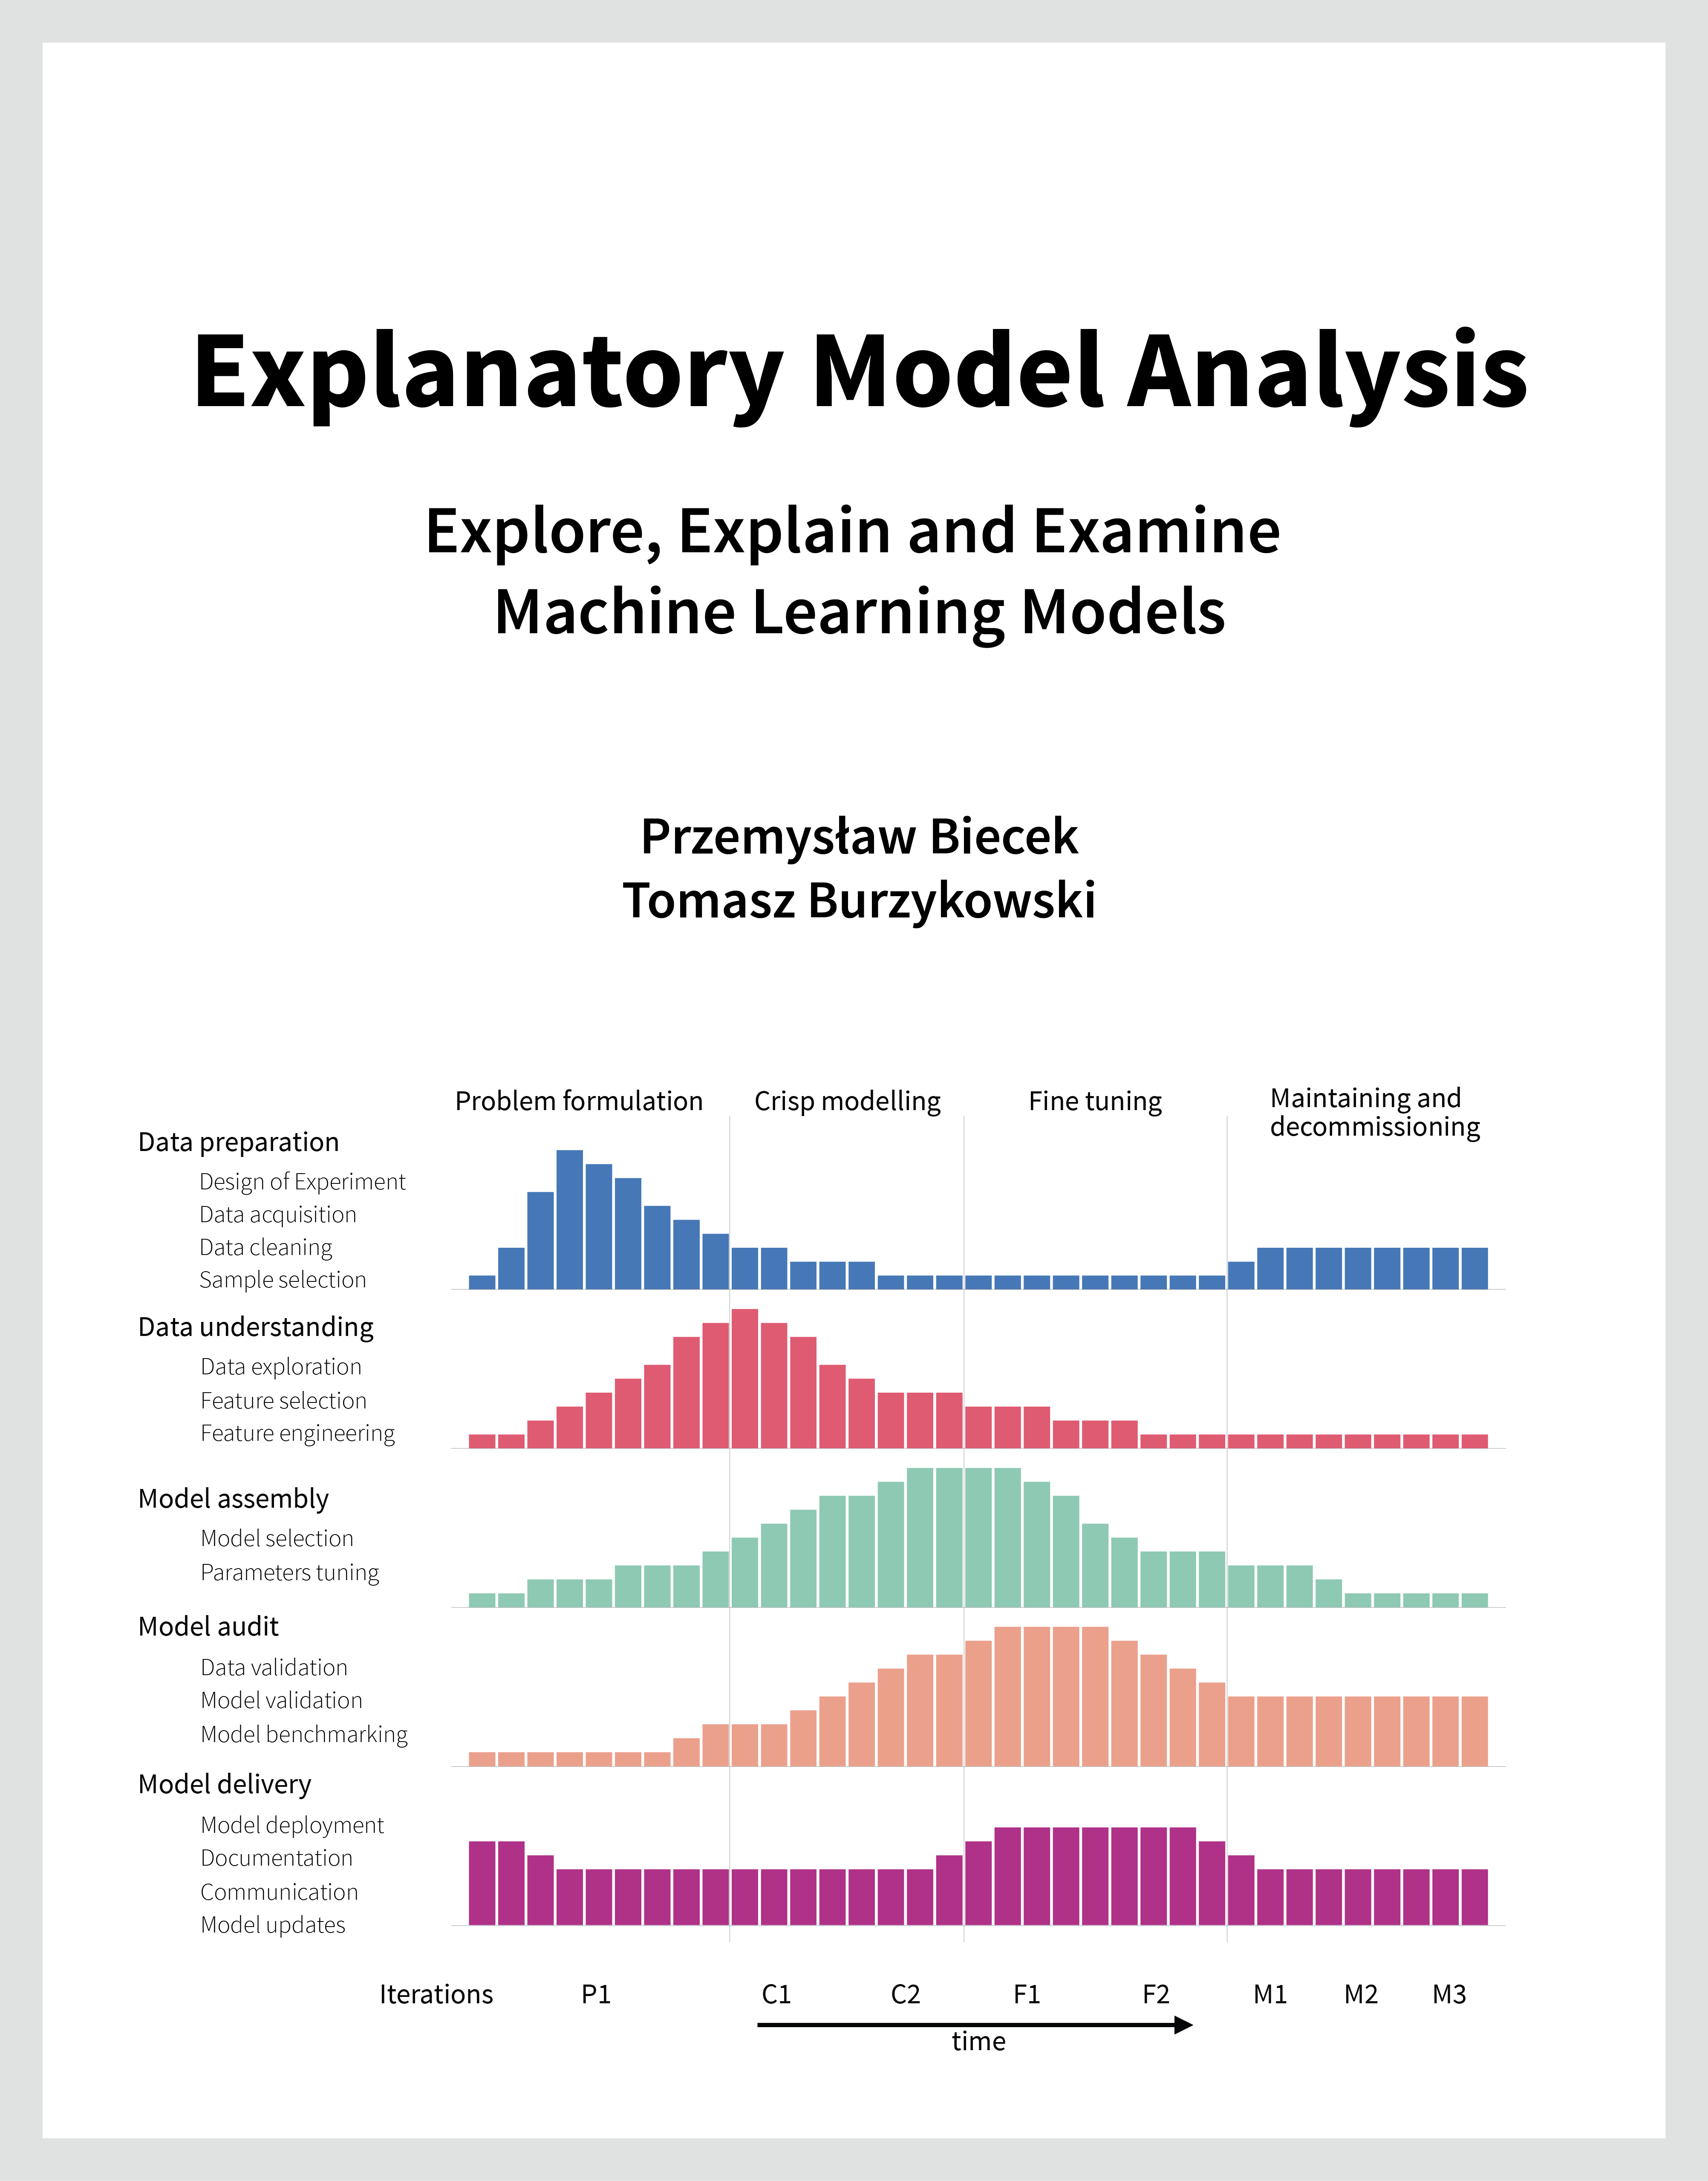
\includegraphics[width=0.99\linewidth]{figure/front} \end{center}

\hypertarget{introduction}{%
\section{Introduction}\label{introduction}}

\hypertarget{notes-to-readers}{%
\subsection{Notes to readers}\label{notes-to-readers}}

A note to readers: this text is a work in progress.

We've released this initial version to get more feedback. Feedback can be given at the GitHub repo \url{https://github.com/pbiecek/PM_VEE/issues}. Copyediting has not been done yet so read at your own risk.

We are primarily interested in the organization and consistency of the content, but any comments will be welcommed.

Thanks for taking the time to read this.

We'd like to thank everyone that contributed feedback, typos, or discussions while the book was being written. GitHub contributors included, \href{https://github.com/agosiewska/}{agosiewska}, Rees Morrison, \href{https://github.com/kasiapekala/}{kasiapekala}, \href{https://github.com/hbaniecki/}{hbaniecki}, \href{https://github.com/AsiaHenzel/}{AsiaHenzel}.

\hypertarget{the-aim-of-the-book}{%
\subsection{The aim of the book}\label{the-aim-of-the-book}}

Predictive models are used to guess (statisticians would say: predict) values of a variable of interest based on other variables. As an example, consider prediction of sales based on historical data, prediction of risk of heart disease based on patient characteristics, or prediction of political attitudes based on Facebook comments.

Predictive models have been constructed through the enitre human history. Ancient Egyptians, for instance, used observations of the rising of Sirius to predict flooding of the Nile. A more rigorous approach to model construction may be attributed to the method of least squares, published more than two centuries ago by Legendre in 1805 and by Gauss in 1809. With time, the number of applications in economy, medicine, biology, and agriculture has grown. The term \emph{regression} was coined by Francis Galton in 1886. Initially, it was referring to biological applications, while today it is used for various models that allow prediction of continuous variables. Prediction of nominal variables is called \emph{classification}, and its beginning may be attributed to works of Ronald Fisher in 1936.

During the last century, many statistical models that can be used for predictive purposes have been developed. These include linear models, generalized linear models, regression and classification trees, rule-based models, and many others. Developments in mathematical foundations of predictive models were boosted by increasing computational power of personal computers and availability of large datasets in the era of ,,big data'' that we have entered.

With the increasing demand for predictive models, model features such as flexibility, ability to perform internally variable selection (feature engineering), and high precision of predictions are of interest. To obtain robust models, ensembles of models are used. Techniques like bagging, boosting, or model stacking combine hundreds or thousands of small models into a one super-model. Large deep neural models have over a billion parameters.

There is a cost of this progress. Complex models may seem to operate like ,,black boxes'`. It may be difficult, or even impossible, to understand how thousands of coefficients affect the model prediction. At the same time, complex models may not work as well as we would like them to. An overview of real problems with large black-box models may be found in an excellent book of Cathy O'Neil \citep{ONeil} or in her TED Talk ,,\emph{The era of blind faith in big data must end}''. There is a growing number of examples of predictive models with performance that deteriorated over time or became biased in some sense. For instance, IBM's Watson for Oncology was criticized by oncologists for delivering unsafe and inaccurate recommendations \citep{IBMWatson}. Amazon's system for CV screening was found to be biased against women \citep{AmazonAI}. The COMPAS (Correctional Offender Management Profiling for Alternative Sanctions) algorithm for predicting recidivism, developed by Northpointe (now Equivant), is biased against blacks \citep{COMPAS}. These are examples of models and algorithms that led to serious violations of fairness and ethical principles. An example of situation when data drift led to deterioration in model performance is the Google Flu model, which gave worse predictions after two years than at baseline \citep{GoogleFLU}, {[}Lazer et al Science 2014{]}.

A reaction to some of these examples and problems are new regulations, like the General Data Protection Regulation \citep{EUGDPR}. Also, new civic rights are being formulated \citep{RightToExpl}, \citep{RightToExpl2}, \citep{RightToExpl3}. A noteworthy example is the \emph{,,Right to Explanation''}, i.e., the right to be provided an explanation for an output of an automated algorithm \citep{RightToExpl}. To exercise the right, methods for verification, exploration, and explanation of predictive models are needed.

We can conclude that, today, the true bottleneck in predictive modelling is not the lack of data, nor the lack of computational power, nor inadequate algorithms, nor the lack of flexible models. It is the lack of tools for model validation, model exploration, and explanation of model decisions. Thus, in this book, we present a collection of methods that may be used for this purpose. As development of such methods is a very active area of research and new methods become available almost on a continuous basis, we do not aim at being exhaustive. Rather, we present the mind-set, key problems, and several examples of methods that can be used in model exploration.

\begin{figure}

{\centering 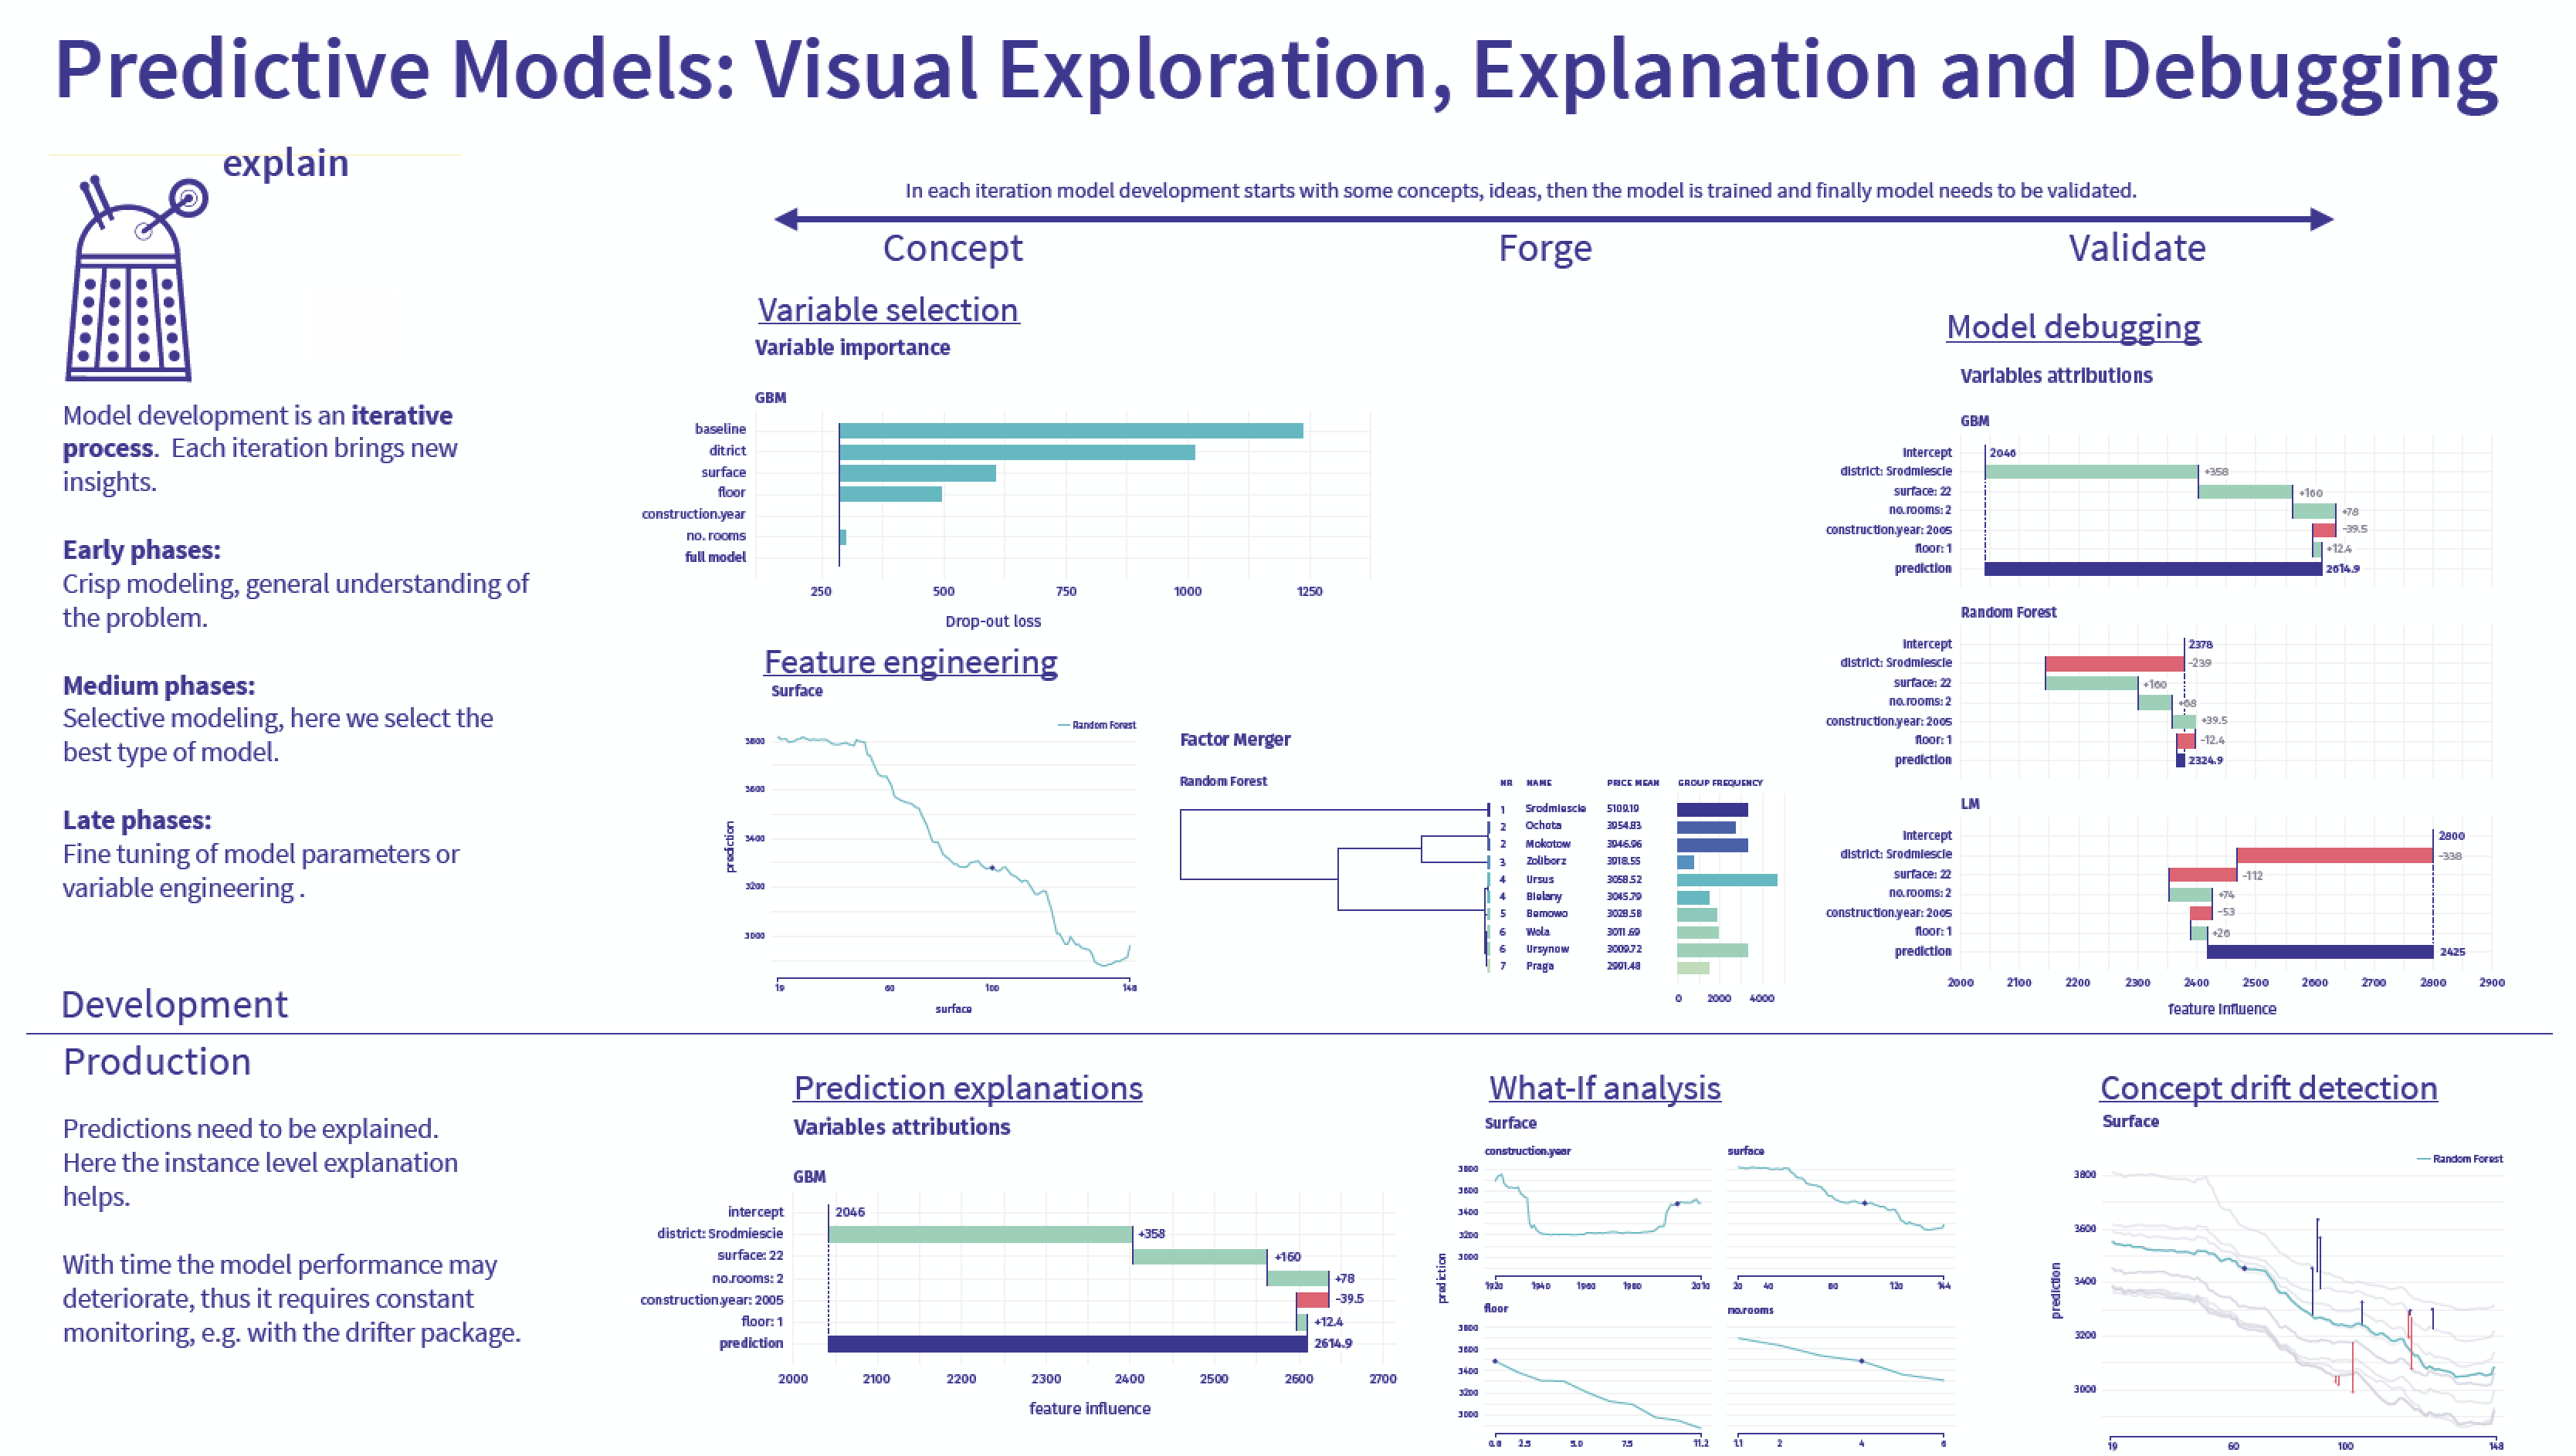
\includegraphics[width=0.99\linewidth]{figure/DrWhyAI_PMVEE} 

}

\caption{(fig:DrWhyAIPMVEE) Visual exploration of predictive models help in every phase of model life-cycle. Model level methods help in early crisp modeling. Instance level methods help in debugging. Feature effects help to cross-compare candidate models. Auditors help to identify weak sides of considered models.}\label{fig:DrWhyAIPMVEE}
\end{figure}

\hypertarget{three-single-laws}{%
\subsection{A bit of philosophy: three laws of model explanation}\label{three-single-laws}}

Seventy-six years ago, Isaac Asimov forumlated \href{https://en.wikipedia.org/wiki/Three_Laws_of_Robotics}{Three Laws of Robotics}:
1) a robot may not injure a human being,
2) a robot must obey the orders given it by human beings, and
3) a robot must protect its own existence.

Today's robots, like cleaning robots, robotic pets, or autonomous cars are far from being conscious enough to fall under Asimov's ethics. However, we are more and more surrounded by complex predictive models and algorithms used for decision making. Machine-learning models are used in health care, politics, education, justice, and many other areas. The models and algorithms have a far larger influence on our lives than physical robots. Yet, applications of such models are left unregulated despite examples of their potential harmfulness. See \emph{Weapons of Math Destruction} by Cathy O'Neil \citep{ONeil} for an excellent overview of selected problems.

It's clear that we need to control the models and algorithms that may affect us. Thus, Asimov's laws are referred to in the context of the discussion around \href{https://en.wikipedia.org/wiki/Ethics_of_artificial_intelligence}{Ethics of Artifical Intelligence}. Initiatives to formulate principles for AI development have been undertaken, for instance, in the UK {[}Olhede \& Wolfe, Significance 2018, 15: 6-7{]}. Following Asimov's approach, we propose three requirements that any predictive model should fulfill:

\begin{itemize}
\tightlist
\item
  \textbf{Prediction's justification}. For every prediction of a model, one should be able to understand which variables affect the prediction and to what extent.
\item
  \textbf{Prediction's speculation}. For every prediction of a model, one should be able to understand how the model prediction would change if input variables changed.
\item
  \textbf{Prediction's validation}. For every prediction of a model, one should be able to verify how strong is the evidence that confirms the prediction.
\end{itemize}

We see two ways to comply with these requirements. One is to use only models that fulfill these conditions by design. However, the price for transparency may be a reduction in performance. Another way is to use tools that allow, perhaps by using approximations, to ,,explain'' predictions for any model. In our book, we will focus on the latter approach.

\hypertarget{terminology}{%
\subsection{Terminology}\label{terminology}}

It is worth noting that, when it comes to predictive models, the same concepts have often been given different names in statistics and in machine learning. For instance, in the statistical-modelling literature, one refers to ,,explanatory variables,'' with ,,independent variables,'' ,,predictors,'' or ,,covariates'' as often-used equivalents. Explanatory variables are used in the model as means to explain (predict) the ,,dependent variable,'' also called ,,predicted'' variable or ,,response.'' In machine-learning terminology, ,,input variables'' or ,,features'' are used to predict the ,,output'' variable. In statistical modelling, models are fit to the data that contain ,,observations,'' whereas in the machine-learning world a dataset may contain ,,instances'`. When we talk about values that defines a single instance of a model in statistical modelling we refer to model ,,coefficients'' while in machine-learning it is more common to use phrase model ,,parameters''.

To the extent possible, in our book we try to consistently use the statistical-modelling terminology. However, the reader may find references to a ,,feature'' here and there. Somewhat inconsistently, we also introduce the term ,,instance-level'' explanation. Instance-level explanation methods are designed to extract information about the behavior of the model related to a specific observation (or instance). On the other hand, ,,global'' explanation techniques allow obtaining information about the behavior of the model for an entire dataset.

We consider models for dependent variables that can be continuous or nominal. The values of a continuous variable can be represented by numbers with an ordering that makes some sense (zip codes or phone numbers are not considered as continuous variables). A continuous variable does not have to be continuous in the mathematical sense; counts (number of floors, steps, etc.) will be treated as continuous variables as well. A nominal variable can assume only a finite set of values that cannot be given numeric values.

In this book we focus on ,,black-box'' models. We discuss them in a bit more detail in the next section.

\hypertarget{glass-box-models-vs.black-box-models}{%
\subsection{Glass-box models vs.~black-box models}\label{glass-box-models-vs.black-box-models}}

Black-box models are models with a complex structure that is hard to understand by humans. Usually this refers to a large number of model coefficients. As people vary in their capacity to understand complex models, there is no strict threshold for the number of coefficients that makes a model a black-box. In practice, for most people this threshold is probably closer to 10 than to 100.

A ,,glass-box'' (sometimes called white-box) model, which is opposite to a ,,black-box'' one, is a model that is easy to understand (though maybe not by every person). It has a simple structure and a limited number of coefficients. The two most common classess of glass-box models are decision or regression trees, as an example in Figure \ref{fig:BILLCD8}, or models with an additive structure, like the following model for mortality risk in melanoma patients:

\[
RelativeRisk = 1 + 3.6 * [Breslow > 2] - 2 * [TILs > 0] 
\]

In the model, two explanatory variables are used: an indicator whether the thickness of the lesion according to the Breslow scale is larger than 2 mm and an indicator whether the percentage of tumor-infiltrating lymphocytes (TILs) is larger than 0.

The structure of a glass box-model is, in general, easy to understand. It may be difficult to collect the necessary data, build the model, fit it to the data, or perform model validation, but once the model has been developed its interpretation and mode of working is straightforward.

Why is it important to understand the model structure? There are several important advantages. If the model structure is clear, we can easily see which variables are included in the model and which are not. Hence, for instance, we may be able to, question the model when a particular explanatory variable was excluded from it. Also, in the case of a model with a clear structure and a limited number of coefficients, we can easily link changes in model predictions with changes in particular explanatory variables. This, in turn, may allow us to challenge the model against domain knowledge if, for instance, the effect of a particular variable on predictions is inconsistent with previously established results. Note that linking changes in model predictions with changes in particular explanatory variables may be difficult when there are many variables and/or coefficients in the model. For instance, a classification tree with hundreds of nodes is difficult to understand, as is a linear regression model with hundreds of cofficients.

Comprehending the performance of a black-box models presents more challenges. The structure of a complex model, such as a neural-network model, mmay be far from transparent. Consequently, we may not understand which features influence the model decisions and bby how much. Consequently, it may be difficult to decide whether the model is consistent with our domain knowledge. In our book we present tools that can help in extracting the information necessary for the evaluation of complex models.

\begin{figure}

{\centering 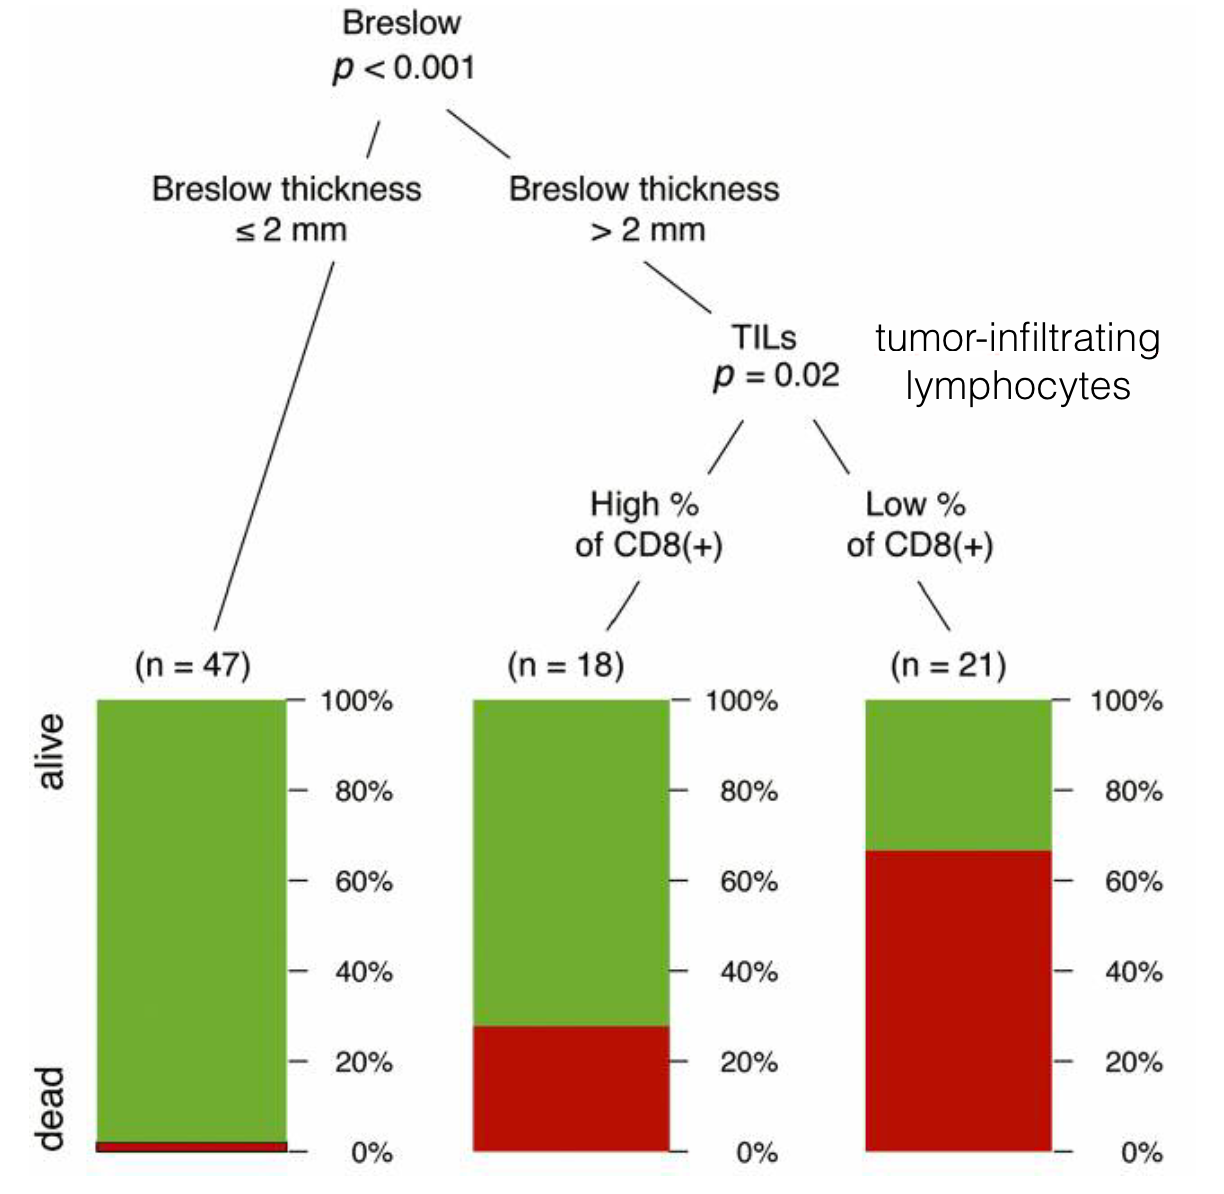
\includegraphics[width=0.5\linewidth]{figure/wbBILL8model} 

}

\caption{(fig:BILLCD8) Example tree model for melanoma risk}\label{fig:BILLCD8}
\end{figure}

\hypertarget{model-visualization-exploration-and-explanation}{%
\subsection{Model visualization, exploration, and explanation}\label{model-visualization-exploration-and-explanation}}

In general, the lifecycle of a model can be divided, into three phases: development (or building), deployment, and maintenance.

Model development is the phase in which one is looking for the best available model. During this process, model exploration tools are useful. Exploration involves evaluation of the fit of the model, verification of the assumptions underlying the model (diagnostics), and assessment of the predictive performance of the model (validation). In our book we will focus on the visualization tools that can be useful in model exploration. We will not, however, discuss visualization methods for diagnostic purposes, as they are extensively discussed in many books devoted to statistical modelling.

Model deployment is the phase in which a predictive model is adopted for use. In this phase, it is crucial that the users gain confidence in using the model. It is worth noting that the users might not have been involved in the model development. Moreover, they may only have access to the binary implementation of the model, may not provide any insight into the details of the model structure. In this situation, model explanation tools can help to understand the factors that influence model predictions and boost confidence in the model. The tools are one of the main focus points of our book.

Finally, a deployed model requires maintenance. In this phase, one monitors a model performance by, for instance, checking the validity of predictions for different datasets. If issues are detected, model explanation tools may be used to find the source of the problem and to suggest a modification of the structure of the model.

\hypertarget{model-agnostic-vs.model-specific-approach}{%
\subsection{Model-agnostic vs.~model-specific approach}\label{model-agnostic-vs.model-specific-approach}}

Some classes of models have been developed for a long period of time or have attracted intensive research. Consequently, those classes of models are equipped with excellent tools for model exploration or visualisation. For example:

\begin{itemize}
\tightlist
\item
  There are many tools for diagnostics and evaluation of linear models. Model assumptions are formally defined (normality, linear structure, homogenous variance) and can be checked by using normality tests or plots (normal qq-plot), diagnostic plots, tests for model structure, tools for identification of outliers, etc.
\item
  For many more advanced models with an additive structure, like the proportional hazards model, many tools can be used for checking model assumptions.
\item
  Random-forest models are equipped with the out-of-bag method of evaluating performance and several tools for measuring variable importance \citep{R-randomForest}. Methods have been developed to extract information from the model structure about possible interactions \citep{randomForestExplainer}. Similar tools have been developed for other ensembles of trees, like xgboost models \citep{xgboostExplainer}.
\item
  Neural networks enjoy a large collection of dedicated model-explanation tools that use, for instance, the layer-wise relevance propagation technique \citep{BachLWRP}, or saliency maps technique \citep{SaliencyMaps}, or a mixed approach.
\end{itemize}

Of course, the list of model classes with dedicated collections of model-explanation and/or diagnostics methods is much longer. This variety of model-specific approaches does lead to issues, though. For instance, one cannot easily compare explanations for two models with different structures. Also, every time a new architecture or a new ensemble of models is proposed, one needs to look for new methods of model exploration. Finally, for brand-new models no tools for model explanation or diagnostics may be immediately available.

For these reasons, in our book we focus on model-agnostic techniques. In particular, we prefer not to assume anything about the model structure, as we may be dealing with a black-box model with an unclear structure. In that case, the only operation that we may be able to perform is evaluation of a model for a selected observation.

However, while we do not assume anything about the structure of the model, we will assume that the model operates on \(p\)-dimensional vectors and, for a single vector, it returns a single value which is a real number. This assumption holds for a broad range of models for data such as tabular data, images, text data, videos, etc. It may not be suitable for, e.g., models with memory like seq2seq models \citep{seq2seq} or Long Short Term Memory models \citep{lstm} in which the model output depends also on sequence of previous inputs.

\hypertarget{notation}{%
\subsection{Notation}\label{notation}}

Methods described in this book were developed by different authors, who used different mathematical notations.
We try to keep the mathematical notation consistent throughout the entre book. In some cases this may result in formulae with a fairly complex system of indices.

In this section, we provide a general overview of the notation we use. Whenever necessary, parts of the notation will be explained again in subsequent chapters.

We consider predictive models that operate on a \(p\)-dimensional input space \(\mathcal X\). By \(x \in \mathcal X\) we will refer to a single point in this input space.

In some cases models are described in context of a dataset with \(n\) observations. By \(x_i\) we refer to the \(i\)-th observation in this dataset. Of course, \(x_i \in \mathcal X\).

Some explainers are constructed around an observation of interest which will be denoted by \(x_{*}\). The observation may not necessarily belong to the analyzed dataset; hence, the use of the asterisk in the index. Of course, \(x_* \in \mathcal X\).

Points in \(\mathcal X\) are \(p\) dimensional vectors. We will refer to the \(j\)-th coordinate by using \(j\) in superscript. Thus, \(x^j_i\) deontes the \(j\)-th coordinate of the \(i\)-th observation from the analyzed dataset. If \(\mathcal J\) denotes a subset of indices, then \(x^{\mathcal J}\) denotes the elements of vector \(x\) corresponding to the indices included in \(\mathcal J\).

We will use the notation \(x^{-j}\) to refer to a vector that results from removing the \(j\)-th coordinate from vector \(x\). By \(x^{j|=z}\), we denote a vector with the values at all coordinates equal to the values in \(x\), except of the \(j\)-th coordinate, which is set equal to \(z\). So, if \(w=x^{j|=z}\), then \(w^j = z\) and \(\forall_{k\neq j} w^k = x^k\).

In this book, a model is a function \(f:\mathcal X \rightarrow y\) that transforms a point from \(\mathcal X\) into a real number. In most cases, the presented methods can be used directly for multi-variate dependent variables; however, we use examples with uni-variate responses to simplify the notation.

We will use \(r_i = y_i - f(x_i)\) we refer to the model residual, i.e., the difference between the observed value of the dependent variable \(Y\) for the \(i\)-th observation from a particular dataset and the model prediction for the observaton.

\hypertarget{bookstructure}{%
\subsection{The structure of the book}\label{bookstructure}}

Our book is split in two parts. In the part \emph{Instance-level explainers}, we present techniques for exploration and explanation of model predictions for a single observation. On the other hand, in the part \emph{Global explainers}, we present techniques for exploration and explanation of model's performance for an entire dataset.

Before embarking on the description of the methods, in Chapter \ref{doItYourselfWithR}, we provide a short description of R tools and packages that are necessary to replicate the results presented for various methods. In Chapter \ref{dataSetsIntro}, we describe three datasets that are used throughout the book to illustrate the presented methods and tools.

The \emph{Instance-level explainers} part of the book consists of Chapters \ref{ceterisParibus}-\ref{SummaryInstanceLevel}. In Chapters \ref{ceterisParibus}-\ref{localDiagnostics}, methods based on Ceteris-paribus (CP) profiles are presented. The profiles show the change of model-based predictions induced by a change of a single variable; they are introduced in Chapter \ref{ceterisParibus}. Chapter \ref{ceterisParibusOscillations} presents a CP-profile-based measure that summarizes the impact of a selected variable on model's predictions. The measure can be used to select the profiles that are worth plotting for a model with a large number of explanatory variables. Chapter \ref{localDiagnostics} describes local-fidelity plots that are useful to investigate the sources of a poor prediction for a particular single observation.

Chapters \ref{breakDown}-\ref{shapley} present methods to decompose variable contributions to model predictions. In particular, Chapter \ref{breakDown} introduces Break-down (BD) plots for models with additive effects. On the other hand, Chapter \ref{iBreakDown} presents a method for models including interactions. Finally, Chapter \ref{shapley} describes an alternative method for decomposing model predictions that is closely linked with Shapley values \citep{shapleybook1952} developed originally for cooperative games.

Chapter \ref{LIME} presents a different approach to explanation of single-instance predictions. It is based on a local approximation of a black-box model by a simpler, glass-box one. In paricular, in the chapter, the Local Interpretable Model-Agnostic Explanations (LIME) method \citep{lime} is discussed.

The final chapter of the first part, Chapter \ref{SummaryInstanceLevel}, presence a comparison of various instance-level explainers.

The \emph{Global explainers} part of the book consists of Chapters \ref{ModelLevelExploration}-\ref{conceptDrift}.

In each part, every method is described in a separate chapter that has the same structure:
* Subsection \emph{Introduction} explains the goal of and the general idea behind the method.
* Subsection \emph{Method} shows mathematical or computational details related to the method. This subsection can be skipped if you are not interested in the details.
* Subsection \emph{Example} shows an exemplary application of the method with discussion of results.
* Subsection \emph{Pros and cons} summarizes the advantages and disadvantages of the method. It also provides some guideance regarding when to use the method.
* Subsection \emph{Code snippets} shows the implementation of the method in R and Python. This subsection can be skipped if you are not interested in the implementation.

Finally, we would like to signal that, \textbf{in this book, we do show}

\begin{itemize}
\tightlist
\item
  how to determine features that affect model prediction for a single observation. In particular, we present the theory and examples of methods that can be used to explain prediction like break down plots, ceteris paribus profiles, local-model approximations, or Shapley values.
\item
  techniques to examine fully-trained machine-learning models as a whole. In particular, we review the theory and examples of methods that can be used to explain model performance globally, like partial-dependency plots, variable-importance plots, and others.
\item
  charts that can be used to present key information in a quick way.
\item
  tools and methods for model comparison.
\item
  code snippets for R and Python that explain how to use the described methods.
\end{itemize}

On the other hand, \textbf{in this book, we do not focus on}

\begin{itemize}
\tightlist
\item
  any specific model. The techniques presented are model agnostic and do not make any assumptions related to model structure.
\item
  data exploration. There are very good books on this topic, like R for Data Science \url{http://r4ds.had.co.nz/} or TODO
\item
  the process of model building. There are also very good books on this topic, see An Introduction to Statistical Learning by Gareth James, Daniela Witten, Trevor Hastie and Robert Tibshirani \url{http://www-bcf.usc.edu/~gareth/ISL/} or TODO
\item
  any particular tools for model building. These are discussed, for instance, in Applied Predictive Modeling by Max Kuhn and Kjell Johnson \url{http://appliedpredictivemodeling.com/}
\end{itemize}

\hypertarget{thanksto}{%
\subsection{Acknowledgements}\label{thanksto}}

Przemek's work on interpretability started during research trips within the RENOIR project (691152 - H2020/2016-2019). So he would like to thank Prof.~Janusz Holyst for the chance to take part in this project.

Przemek would also like thank Prof.~Chris Drake for her hospitality. This book would have never been created without perfect conditions that Przemek found at Chris's house in Woodland.

This book has been prepared using the \textbf{bookdown} package \citep{R-bookdown}, created thanks to the amazing work of Yihui Xie.

\hypertarget{doItYourselfWithR}{%
\section{Do-it-yourself With R}\label{doItYourselfWithR}}

In our book we introduce different methods for instance-level and global explanation and exploration of predictive models. In each chapter, there is a section with code snippets for R that show how a particular method has been implemented. In this chapter we provide a short description of steps that will allow the reader to replicate the results presented for various methods.

\hypertarget{what-to-install}{%
\subsection{What to install?}\label{what-to-install}}

Obviously, R \citep{RcoreT} is needed. It is always better to use the newest version, but at least R in version 3.5 should be used. R can be downloaded from \url{https://cran.r-project.org/}.

A good editor makes working with R much easier. There is a plenty of choices, but, especially for beginners, it is worth considering the RStudio editor, an open-source and enterprise-ready tool for R. It can be downloaded from \url{https://www.rstudio.com/}.

Once R and the editor are available, the required packages should be installed.

The most important one is the \texttt{DALEX} package. It is the entry point to solutions introduced in this book. The package can be installed by executing the following command from the R command line:

\begin{verbatim}
install.packages("DALEX")
\end{verbatim}

Installation of \texttt{DALEX} will automatically take care about installation of other hard requirements (packages required by it), like the \texttt{ggplot2} package for data visualization.

To repeat all examples in this book, two additional packages are needed: \texttt{ingredients} and \texttt{iBreakDown}. The easiest way to get them, including other useful weak dependencies, is to execute the following command:

\begin{verbatim}
DALEX::install_dependencies()
\end{verbatim}

\hypertarget{how-to-work-with-dalex}{%
\subsection{\texorpdfstring{How to work with \texttt{DALEX}?}{How to work with DALEX?}}\label{how-to-work-with-dalex}}

To conduct model exploration with \texttt{DALEX}, first, a model has to be created. Then the model has got to be prepared for exploration.

There are many packages in R that can be used to construct a model. Some packages are structure-specific, like \texttt{randomForest} for Random-Forest Classification and Regression models \citep{randomForest}, \texttt{gbm} for Generalized Boosted Regression Models \citep{gbm}, extensions for Generalized Linear Models \citep{rms}, or many others. There is also a number of packages that can be used for constucting models with different structures. These include the \texttt{h2o} package \citep{h2oPackage}, \texttt{caret} \citep{caret} and its successor \texttt{parsnip} \citep{parsnipPackage}, a very powerful and extensible \texttt{mlr} \citep{mlr}, or \texttt{keras} that is a wrapper to Python library with the same name \citep{kerasPackage}.

While it is great to have such a large choice of tools for constructing models, the downside is that different packages have different interfaces and different arguments. Moreover, model-objects created with different packages may have different internal structures. The main goal of the \texttt{DALEX} package \citep{DALEX} is to create a level of abstraction around a model that makes it easier to explore and explain the model.

Function \texttt{DALEX::explain} is THE function for model wrapping. The function requires five arguments:

\begin{itemize}
\tightlist
\item
  \texttt{model}, a model-object;
\item
  \texttt{data}, a data frame with validation data;
\item
  \texttt{y}, observed values of the dependent variable for the validation data; it is an optional argument, required for explainers focused on model validation and benchmarking.
\item
  \texttt{predict\_function}, a function that returns prediction scores; if not specified, then a default \texttt{predict()} function is used. Note that, for some models, the default \texttt{predict()} function returns classes; in such cases you should provide a function that will return numerical scores.
\item
  \texttt{label}, a name of a model; if not specified, then it is extracted from the \texttt{class(model)}. This name will be presented in figures, so it is recommended to make the name informative.
\end{itemize}

For an example, see Section \ref{ExplainersTitanicRCode}.

\hypertarget{how-to-work-with-archivist}{%
\subsection{\texorpdfstring{How to work with \texttt{archivist}?}{How to work with archivist?}}\label{how-to-work-with-archivist}}

As we will focus on exploration of predictive models, we prefer not to waste space nor time on replication of the code necessary for model development. This is where the \texttt{archivist} packages helps.

The \texttt{archivist} package \citep{archivist} is designed to store, share, and manage R objects. We will use it to easily access R models and explainers. To install the package, the following command should be executed in the R command line:

\begin{verbatim}
install.packages("archivist")
\end{verbatim}

Once the package has been installed, function \texttt{aread()} can be used to retrieve R objects from any remote repository. For this book, we use a GitHub repository \texttt{models} hosted at \url{https://github.com/pbiecek/models}. For instance, to download a model with the md5 hash \texttt{ceb40}, the following command has to be executed:

\begin{Shaded}
\begin{Highlighting}[]
\NormalTok{archivist}\OperatorTok{::}\KeywordTok{aread}\NormalTok{(}\StringTok{"pbiecek/models/ceb40"}\NormalTok{)}
\end{Highlighting}
\end{Shaded}

Since the md5 hash \texttt{ceb40} uniquely defines the model, referring to the repository object results in using exactly the same model and the same explanations. Thus, in the subsequent chapters, pre-constructed model explainers will be accessed with \texttt{archivist} hooks. In following sections we will also use \texttt{archivist} hooks in references to datasets.

\hypertarget{Packages}{%
\subsection{DrWhy Packages}\label{Packages}}

Here we present list of arguments in explainers from \texttt{DrWhy} universe.
All explainers use unified set of arguments. All of them are generic with two specific implementations \texttt{*.explainer} and \texttt{*.default}. The first one is working for objects created with \texttt{DALEX::explain()} function.

Common core arguments

\begin{itemize}
\tightlist
\item
  \texttt{x} a model to be explained, or an explainer created with function \texttt{DALEX::explain()}.
\item
  \texttt{data} validation dataset. Used to determine univariate distributions, calculation of quantiles, correlations and so on. It will be extracted from \texttt{x} if it's an explainer.
\item
  \texttt{predict\_function} predict function that operates on the model \texttt{x}. Since the model is a black box, the \texttt{predict\_function} is the only interface to access values from the model. It should be a function that takes at least a model \texttt{x} and \texttt{data} and returns vector of predictions. If model response has more than a single number (like multiclass models) then this function should return a marix/data.frame of the size \texttt{m} x \texttt{d}, where \texttt{m} is the number of observations while \texttt{d} is the dimensionality of model response. It will be extracted from \texttt{x} if it's an explainer.
\item
  \texttt{new\_observation} an observation/observations to be explained. Required for local/instance level explainers. Columns in should correspond to columns in the \texttt{data} argument.
\item
  \texttt{...} other parameters.
\item
  \texttt{label} name of the model. By default it's extracted from the \texttt{class} attribute of the model
\end{itemize}

Function specific arguments

\begin{itemize}
\tightlist
\item
  \texttt{keep\_distributions} if \texttt{TRUE}, then distributions of partial predictions is stored and can be plotted with the generic \texttt{plot()}.
\end{itemize}

\hypertarget{doItYourselfWithPython}{%
\section{Do-it-yourself With Python}\label{doItYourselfWithPython}}

\hypertarget{modelDevelopmentProcess}{%
\section{Model Development}\label{modelDevelopmentProcess}}

\hypertarget{MDPIntro}{%
\subsection{Introduction}\label{MDPIntro}}

In this book we present methods that can be used for exploration of models. But before we can explore a model, first we need to train one.

In this part of the book we overview the process of model development and introduce steps that lead to a model creation. It is not a comprehensive manual ,,how to train a model in 5 steps''. The goal of this chapter is to show what needs to be performed before we can do any diagnostic or exploration of a trained model.

Predictive models are created for different purposes. Sometimes it is a team of data scientists that spend months on a single model that will be used for model scoring in a big financial company. Every detail is important for models that operate on large scale and have long-term consequences. Another time it is an in-house model trained for prediction of a demand for pizza. The model is developed by a single person in few hours. If model will not perform well it will be updated, replaced or removed.

Whatever it is a large model or small one, similar steps are to be taken during model development.

\hypertarget{the-process}{%
\subsection{The Process}\label{the-process}}

Several approaches are proposed in order to describe the process of model development. Their main goal is to standardize the process. And the standardisation is important because it helps to plan resources needed to develop and maintain the model and also to not miss any important phase.

The most known methodology for data science projects is CRISP-DM \citep{crisp1999}, \citep{crisp2019wiki} which is a tool agnostic procedure. The key component of CRISP-DM is the break down of the whole process into six phases: business understanding, data understanding, data preparation, modeling, evaluation and deployment. CRISP-DM is general, it was designed for any data science project. For predictive models some methodologies are introduced in \citep{r4ds2019} and \citep{misconceptions2019}. First is a very simple, focused on interactions between three phases: data transformation, modeling and visualisation.

In this book we use \emph{Model Development Process} described in \citep{mdp2019}. It is motivated by Rational Unified Process for Software Development \citep{rup1998}, \citep{usdp1999}, \citep{spiral1988}. The process is shown in Figure \ref{fig:mdpGeneral}. Model building usually may be decomposed into four phases. First is the problem formulation followed by crisp modeling and find tuning of a model. Once the model is created it needs to be maintained and one day decommissioned.

During each phase some tasks are to be done. Some are related to \emph{Data preparation}. Accessing, cleaning and preparation of the data may be time consuming task. Other tasks are related to \emph{Data understanding}. Visual model exploration and feature engineering is often needed in order to create a good model. During the \emph{Model assembly} consecutive versions of a model are being created and compared. New models are benchmarked and validated during the \emph{Model audit}. \emph{Model delivery} are task needed to put the model into production.

\begin{figure}

{\centering 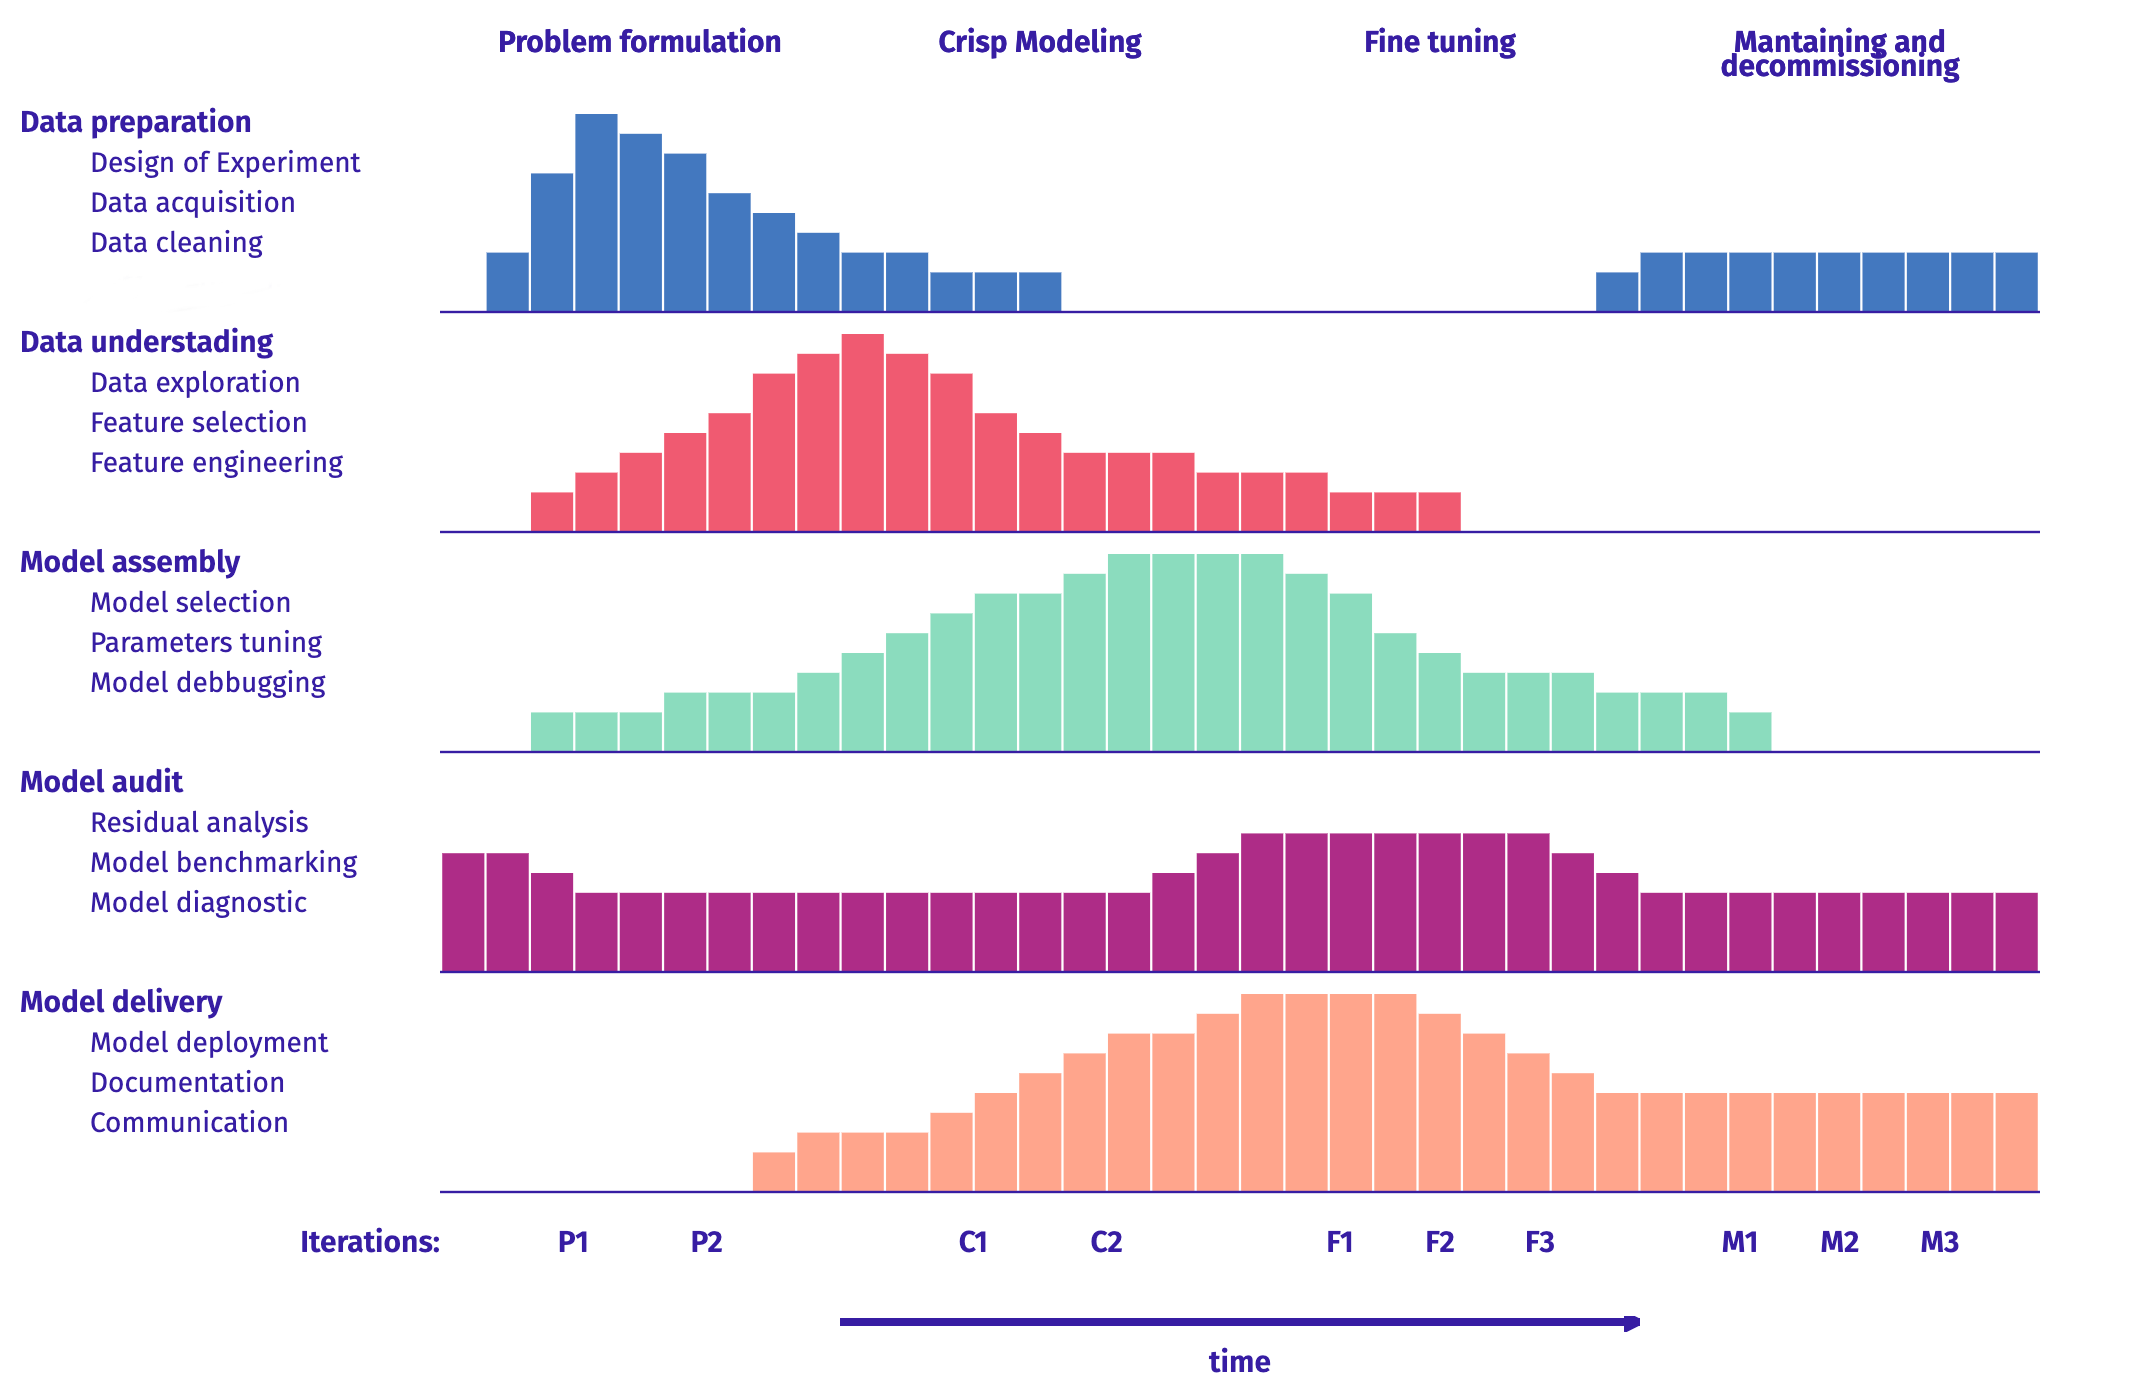
\includegraphics[width=0.99\linewidth]{figure/mdp_general} 

}

\caption{(fig:mdpGeneral) Overview of the Model Development Process. Horizontal axis show how time passes from the problem formulation to the model decommissioning. Vertical axis shows tasks are performed in a given phase. }\label{fig:mdpGeneral}
\end{figure}

\hypertarget{data-preparation}{%
\subsection{Data preparation}\label{data-preparation}}

In many cases the most time consuming phase of model development is the selection and aquisition of the right data.

HERE: MORE DESCRIPTIONS AND REFERENCES ARE NEEDED.

\hypertarget{data-exploration}{%
\subsection{Data exploration}\label{data-exploration}}

Before we start the modeling we need to understand the data.
Visual, tabular and statistical tools for data exploration are used depending on the character of variables.

The most know introduction to data exploration is the famous book by John Tukey \citep{tukey1977}. It introduced new tools for data exploration, like for example boxplots for continuous variables.

Availability of computational tools makes the process of data exploration easier and ore interactive. Find a good overview of techniques for data exploration in \citep{Nolan2015} or \citep{Wickham2017}.

\hypertarget{model-assembly}{%
\subsection{Model assembly}\label{model-assembly}}

Once the data is prepared we can start model assembly.

One can try different algorithms for model training, validation strategies, tuning of hyperparameters. This process is usually iterative and computationally heavy.

Find a good overview of techniques for model development in \citep{Venables2010} or \citep{AppliedPredictiveModeling2013}.

\hypertarget{model-understanding}{%
\subsection{Model understanding}\label{model-understanding}}

Usually the model development starts with some crisp early versions that are refined in consecutive iterations. In order to train a final model we need to try numerous candidate models that will be explored, examined and diagnosed. In this book we will introduce techniques that:

\begin{itemize}
\tightlist
\item
  summarise how good is the current version of a model. Section \ref{modelPerformance} overviews measures for model performance. These measures are usually used to trace the progress in model development.
\item
  assess the feature importance. Section \ref{featureImportance} shows how to assess influence of a single variable on model performance. Features that are not important are usually removed from a model during the model refinement.
\item
  shows how a single feature affects the model response. Sections \ref{partialDependenceProfiles} -- \ref{featureEffects} present Partial Dependency Profiles, Accumulated Local Effects and Marginal Profiles. All these techniques help to understand how model consumes particular features.
\item
  identifies potential problems with a model. Section \ref{residualDiagnostic} shows techniques for exploration of model residuals. Looking closer on residuals often help to improve the model. This is possible with tools for local model exploration which are presented in the fist part of the book.
\item
  performs sensitivity analysis for a model. Section \ref{ceterisParibus} introduces Ceteris Paribus profiles that helps in a what-if analysis for a model.
\item
  validated local fit for a model. Section \ref{localDiagnostics} introduces techniques for assessment if for a single observation the model support its prediction
\item
  decompose model predictions into pieces that can be attributed to particular variables. Sections \ref{breakDown} -- \ref{LIME} show different techniques like SHAP, LIME or Break Down for local exploration of a model.
\end{itemize}

\hypertarget{dataSetsIntro}{%
\section{Data sets and models}\label{dataSetsIntro}}

We illustrate the methods presented in this book by using two datasets:

\begin{itemize}
\tightlist
\item
  \emph{Sinking of the RMS Titanic}
\item
  \emph{Apartment prices}
\end{itemize}

The first dataset will be used to illustrate the application of the techniques in the case of a predictive model for a binary dependent variable. The second one will provide an example for models for a continuous variable.

In this chapter, we provide a short description of each of the datasets, together with results of exploratory analyses. We also introduce models that will be used for illustration purposes in subsequent chapters.

\hypertarget{TitanicDataset}{%
\subsection{Sinking of the RMS Titanic}\label{TitanicDataset}}

\begin{figure}
\centering
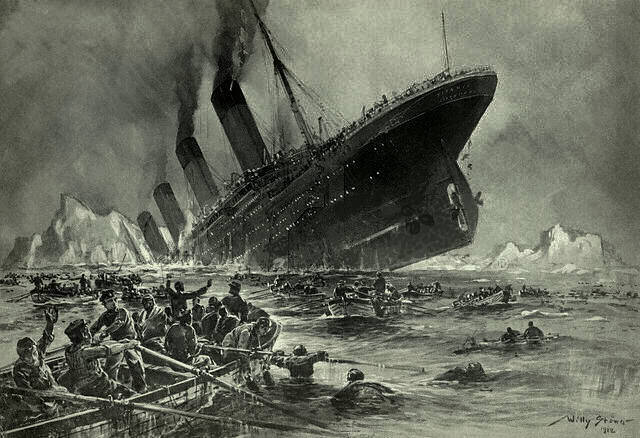
\includegraphics{figure/Titanic.jpg}
\caption{Titanic sinking by Willy Stöwer}
\end{figure}

Sinking of the RMS Titanic is one of the deadliest maritime disasters in history (during peacetime). Over 1500 people died as a consequence of collision with an iceberg. Projects like \emph{Encyclopedia titanica} \texttt{https://www.encyclopedia-titanica.org/} are a source of rich and precise data about Titanic's passengers. The data are available in a dataset included in the \texttt{stablelearner} package. The dataset, after some data cleaning and variable transformations, is also avaliable in the \texttt{DALEX} package. In particular, the `titanic' data frame contains 2207 observations (for 1317 passengers and 890 crew members) and nine variables:

\begin{itemize}
\tightlist
\item
  \emph{gender}, person's (passenger's or crew member's) gender, a factor (categorical variable) with two levels (categories);
\item
  \emph{age}, person's age in years, a numerical variable; for adults, the age is given in (integer) years; for children younger than one year, the age is given as \(x/12\), where \(x\) is the number of months of child's age;
\item
  \emph{class}, the class in which the passenger travelled, or the duty class of a crew member; a factor with seven levels
\item
  \emph{embarked}, the harbor in which the person embarked on the ship, a factor with four levels;
\item
  \emph{country}, person's home country, a factor with 48 levels;
\item
  \emph{fare}, the price of the ticket (only available for passengers; 0 for crew members), a numerical variable;
\item
  \emph{sibsp}, the number of siblings/spouses aboard the ship, a numerical variable;
\item
  \emph{parch}, the number of parents/children aboard the ship, a numerical variable;
\item
  \emph{survived}, a factor with two levels indicating whether the person survived or not.
\end{itemize}

The R code below provides more info about the contents of the dataset, values of the variables, etc.

\begin{Shaded}
\begin{Highlighting}[]
\KeywordTok{library}\NormalTok{(}\StringTok{"DALEX"}\NormalTok{)}
\KeywordTok{head}\NormalTok{(titanic, }\DecValTok{2}\NormalTok{)}
\end{Highlighting}
\end{Shaded}

\begin{verbatim}
##   gender age class    embarked       country  fare sibsp parch survived
## 1   male  42   3rd Southampton United States  7.11     0     0       no
## 2   male  13   3rd Southampton United States 20.05     0     2       no
\end{verbatim}

\begin{Shaded}
\begin{Highlighting}[]
\KeywordTok{str}\NormalTok{(titanic)}
\end{Highlighting}
\end{Shaded}

\begin{verbatim}
## 'data.frame':    2207 obs. of  9 variables:
##  $ gender  : Factor w/ 2 levels "female","male": 2 2 2 1 1 2 2 1 2 2 ...
##  $ age     : num  42 13 16 39 16 25 30 28 27 20 ...
##  $ class   : Factor w/ 7 levels "1st","2nd","3rd",..: 3 3 3 3 3 3 2 2 3 3 ...
##  $ embarked: Factor w/ 4 levels "Belfast","Cherbourg",..: 4 4 4 4 4 4 2 2 2 4 ...
##  $ country : Factor w/ 48 levels "Argentina","Australia",..: 44 44 44 15 30 44 17 17 26 16 ...
##  $ fare    : num  7.11 20.05 20.05 20.05 7.13 ...
##  $ sibsp   : num  0 0 1 1 0 0 1 1 0 0 ...
##  $ parch   : num  0 2 1 1 0 0 0 0 0 0 ...
##  $ survived: Factor w/ 2 levels "no","yes": 1 1 1 2 2 2 1 2 2 2 ...
\end{verbatim}

\begin{Shaded}
\begin{Highlighting}[]
\KeywordTok{levels}\NormalTok{(titanic}\OperatorTok{$}\NormalTok{class)}
\end{Highlighting}
\end{Shaded}

\begin{verbatim}
## [1] "1st"              "2nd"              "3rd"              "deck crew"       
## [5] "engineering crew" "restaurant staff" "victualling crew"
\end{verbatim}

\begin{Shaded}
\begin{Highlighting}[]
\KeywordTok{levels}\NormalTok{(titanic}\OperatorTok{$}\NormalTok{embarked)}
\end{Highlighting}
\end{Shaded}

\begin{verbatim}
## [1] "Belfast"     "Cherbourg"   "Queenstown"  "Southampton"
\end{verbatim}

Models considered for this dataset will use \emph{survived} as the (binary) dependent variable.

\hypertarget{exploration-titanic}{%
\subsubsection{Data exploration}\label{exploration-titanic}}

It is always advisable to explore data before modelling. However, as this book is focused on model exploration, we will limit the data exploration part.

Before exploring the data, we first do some pre-processing. In particular, the value of variables \emph{age}, \emph{country}, \emph{sibsp}, \emph{parch}, and \emph{fare} is missing for a limited number of observations (2, 81, 10, 10, and 26, respectively). Analyzing data with missing values is a topic on its own (Little and Rubin 1987; Schafer 1997; Molenberghs and Kenward 2007). An often-used approach is to impute the missing values. Toward this end, multiple imputation should be considered (Schafer 1997; Molenberghs and Kenward 2007; van Buuren 2012). However, given the limited number of missing values and the intended illustrative use of the dataset, we will limit ourselves to, admittedly inferior, single imputation. In particular, we replace the missing \emph{age} values by the mean of the observed ones, i.e., 30. Missing \emph{country} will be coded by ``X''. For \emph{sibsp} and \emph{parch}, we replace the missing values by the most frequently observed value, i.e., 0. Finally, for \emph{fare}, we use the mean fare for a given \emph{class}, i.e., 0 pounds for crew, 89 pounds for the 1st, 22 pounds for the 2nd, and 13 pounds for the 3rd class. The R code presented below implements the imputation steps.

\begin{Shaded}
\begin{Highlighting}[]
\CommentTok{# missing age is replaced by average (30)}
\NormalTok{titanic}\OperatorTok{$}\NormalTok{age[}\KeywordTok{is.na}\NormalTok{(titanic}\OperatorTok{$}\NormalTok{age)] =}\StringTok{ }\DecValTok{30}
\CommentTok{# missing country is replaced by "X"}
\NormalTok{titanic}\OperatorTok{$}\NormalTok{country <-}\StringTok{ }\KeywordTok{as.character}\NormalTok{(titanic}\OperatorTok{$}\NormalTok{country)}
\NormalTok{titanic}\OperatorTok{$}\NormalTok{country[}\KeywordTok{is.na}\NormalTok{(titanic}\OperatorTok{$}\NormalTok{country)] =}\StringTok{ "X"}
\NormalTok{titanic}\OperatorTok{$}\NormalTok{country <-}\StringTok{ }\KeywordTok{factor}\NormalTok{(titanic}\OperatorTok{$}\NormalTok{country)}
\CommentTok{# missing fare is replaced by class average}
\NormalTok{titanic}\OperatorTok{$}\NormalTok{fare[}\KeywordTok{is.na}\NormalTok{(titanic}\OperatorTok{$}\NormalTok{fare) }\OperatorTok{&}\StringTok{ }\NormalTok{titanic}\OperatorTok{$}\NormalTok{class }\OperatorTok{==}\StringTok{ "1st"}\NormalTok{] =}\StringTok{ }\DecValTok{89}
\NormalTok{titanic}\OperatorTok{$}\NormalTok{fare[}\KeywordTok{is.na}\NormalTok{(titanic}\OperatorTok{$}\NormalTok{fare) }\OperatorTok{&}\StringTok{ }\NormalTok{titanic}\OperatorTok{$}\NormalTok{class }\OperatorTok{==}\StringTok{ "2nd"}\NormalTok{] =}\StringTok{ }\DecValTok{22}
\NormalTok{titanic}\OperatorTok{$}\NormalTok{fare[}\KeywordTok{is.na}\NormalTok{(titanic}\OperatorTok{$}\NormalTok{fare) }\OperatorTok{&}\StringTok{ }\NormalTok{titanic}\OperatorTok{$}\NormalTok{class }\OperatorTok{==}\StringTok{ "3rd"}\NormalTok{] =}\StringTok{ }\DecValTok{13}
\CommentTok{# missing sibsp, parch are replaced by 0}
\NormalTok{titanic}\OperatorTok{$}\NormalTok{sibsp[}\KeywordTok{is.na}\NormalTok{(titanic}\OperatorTok{$}\NormalTok{sibsp)] =}\StringTok{ }\DecValTok{0}
\NormalTok{titanic}\OperatorTok{$}\NormalTok{parch[}\KeywordTok{is.na}\NormalTok{(titanic}\OperatorTok{$}\NormalTok{parch)] =}\StringTok{ }\DecValTok{0}
\end{Highlighting}
\end{Shaded}

After imputing the missing values, we investigate the association between survival status and other variables. Figures \ref{fig:titanicExplorationGender}-\ref{fig:titanicExplorationFare} present graphically the proportion non- and survivors for different levels of the other variables. The height of the bars (on the y-axis) reflects the marginal distribution (proportions) of the observed levels of the variable. On the other hand, the width of the bars (on the x-axis) provides the information about the proportion of non- and survivors. Note that, to construct the graphs for \emph{age} and \emph{fare}, we categorized the range of the observed values.

Figures \ref{fig:titanicExplorationGender} and \ref{fig:titanicExplorationAge} indicate that the proportion of survivors was larger for females and children below 5 years of age. This is most likely the result of the ``women and children first'' principle that is often evoked in situations that require evacuation of persons whose life is in danger. The principle can, perhaps, partially explain the trend seen in Figures \ref{fig:titanicExplorationParch} and \ref{fig:titanicExplorationSibsp}, i.e., a higher proportion of survivors among those with 1-3 parents/children and 1-2 siblings/spouses aboard. Figure \ref{fig:titanicExplorationClass} indicates that passengers travelling in the first and second class had a higher chance of survival, perhaps due to the proximity of the location of their cabins to the deck. Interestingly, the proportion of survivors among crew deck was similar to the proportion of the first-class passengers. Figure \ref{fig:titanicExplorationFare} shows that the proportion of survivors increased with the fare, which is consistent with the fact that the proportion was higher for passengers travelling in the first and second class. Finally, Figures \ref{fig:titanicExplorationEmbarked} and \ref{fig:titanicExplorationCountry} do not suggest any noteworthy trends.

\begin{figure}

{\centering 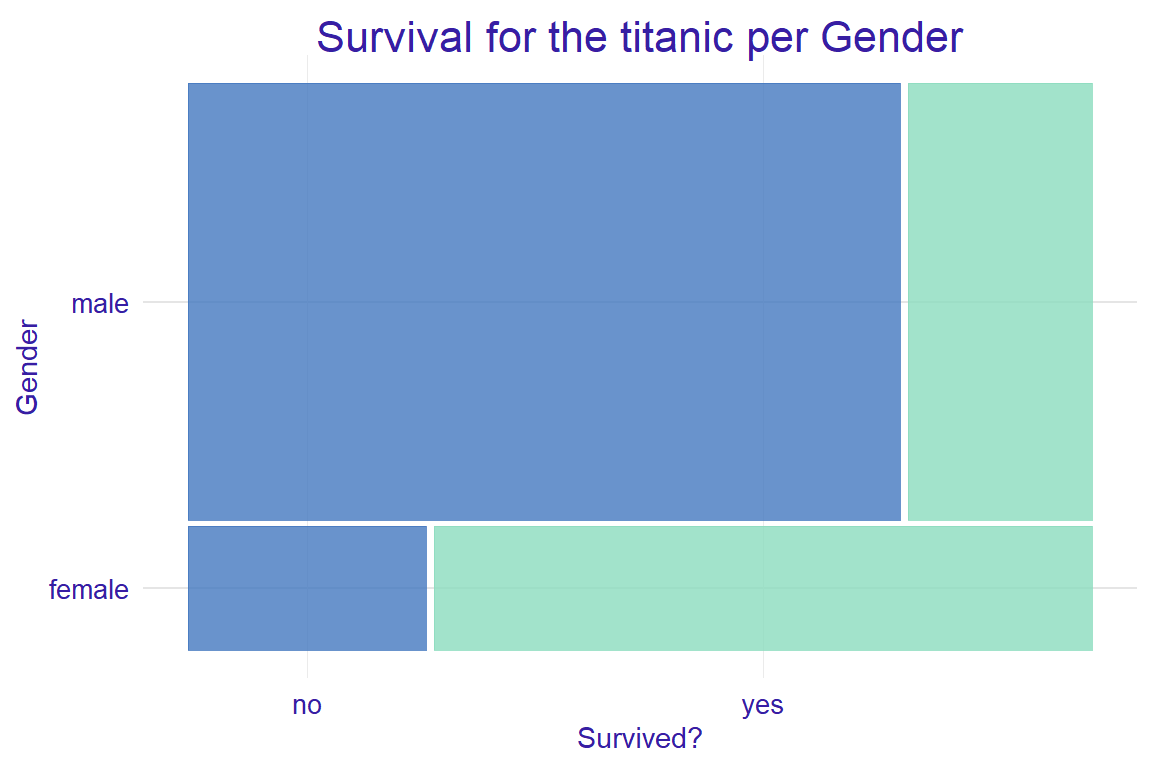
\includegraphics[width=0.7\linewidth]{PM_VEE_files/figure-latex/titanicExplorationGender-1} 

}

\caption{Survival according to gender in the Titanic data.}\label{fig:titanicExplorationGender}
\end{figure}

\begin{figure}

{\centering 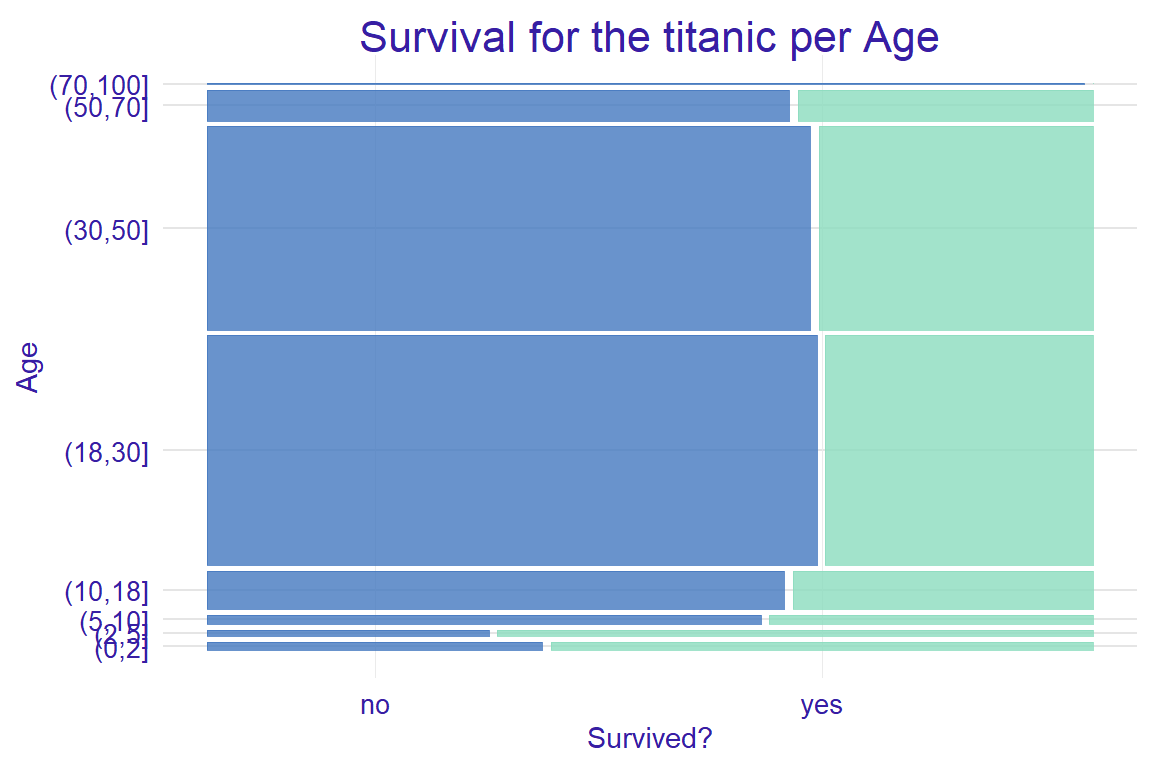
\includegraphics[width=0.7\linewidth]{PM_VEE_files/figure-latex/titanicExplorationAge-1} 

}

\caption{Survival accroding to age group in the Titanic data.}\label{fig:titanicExplorationAge}
\end{figure}

\begin{figure}

{\centering 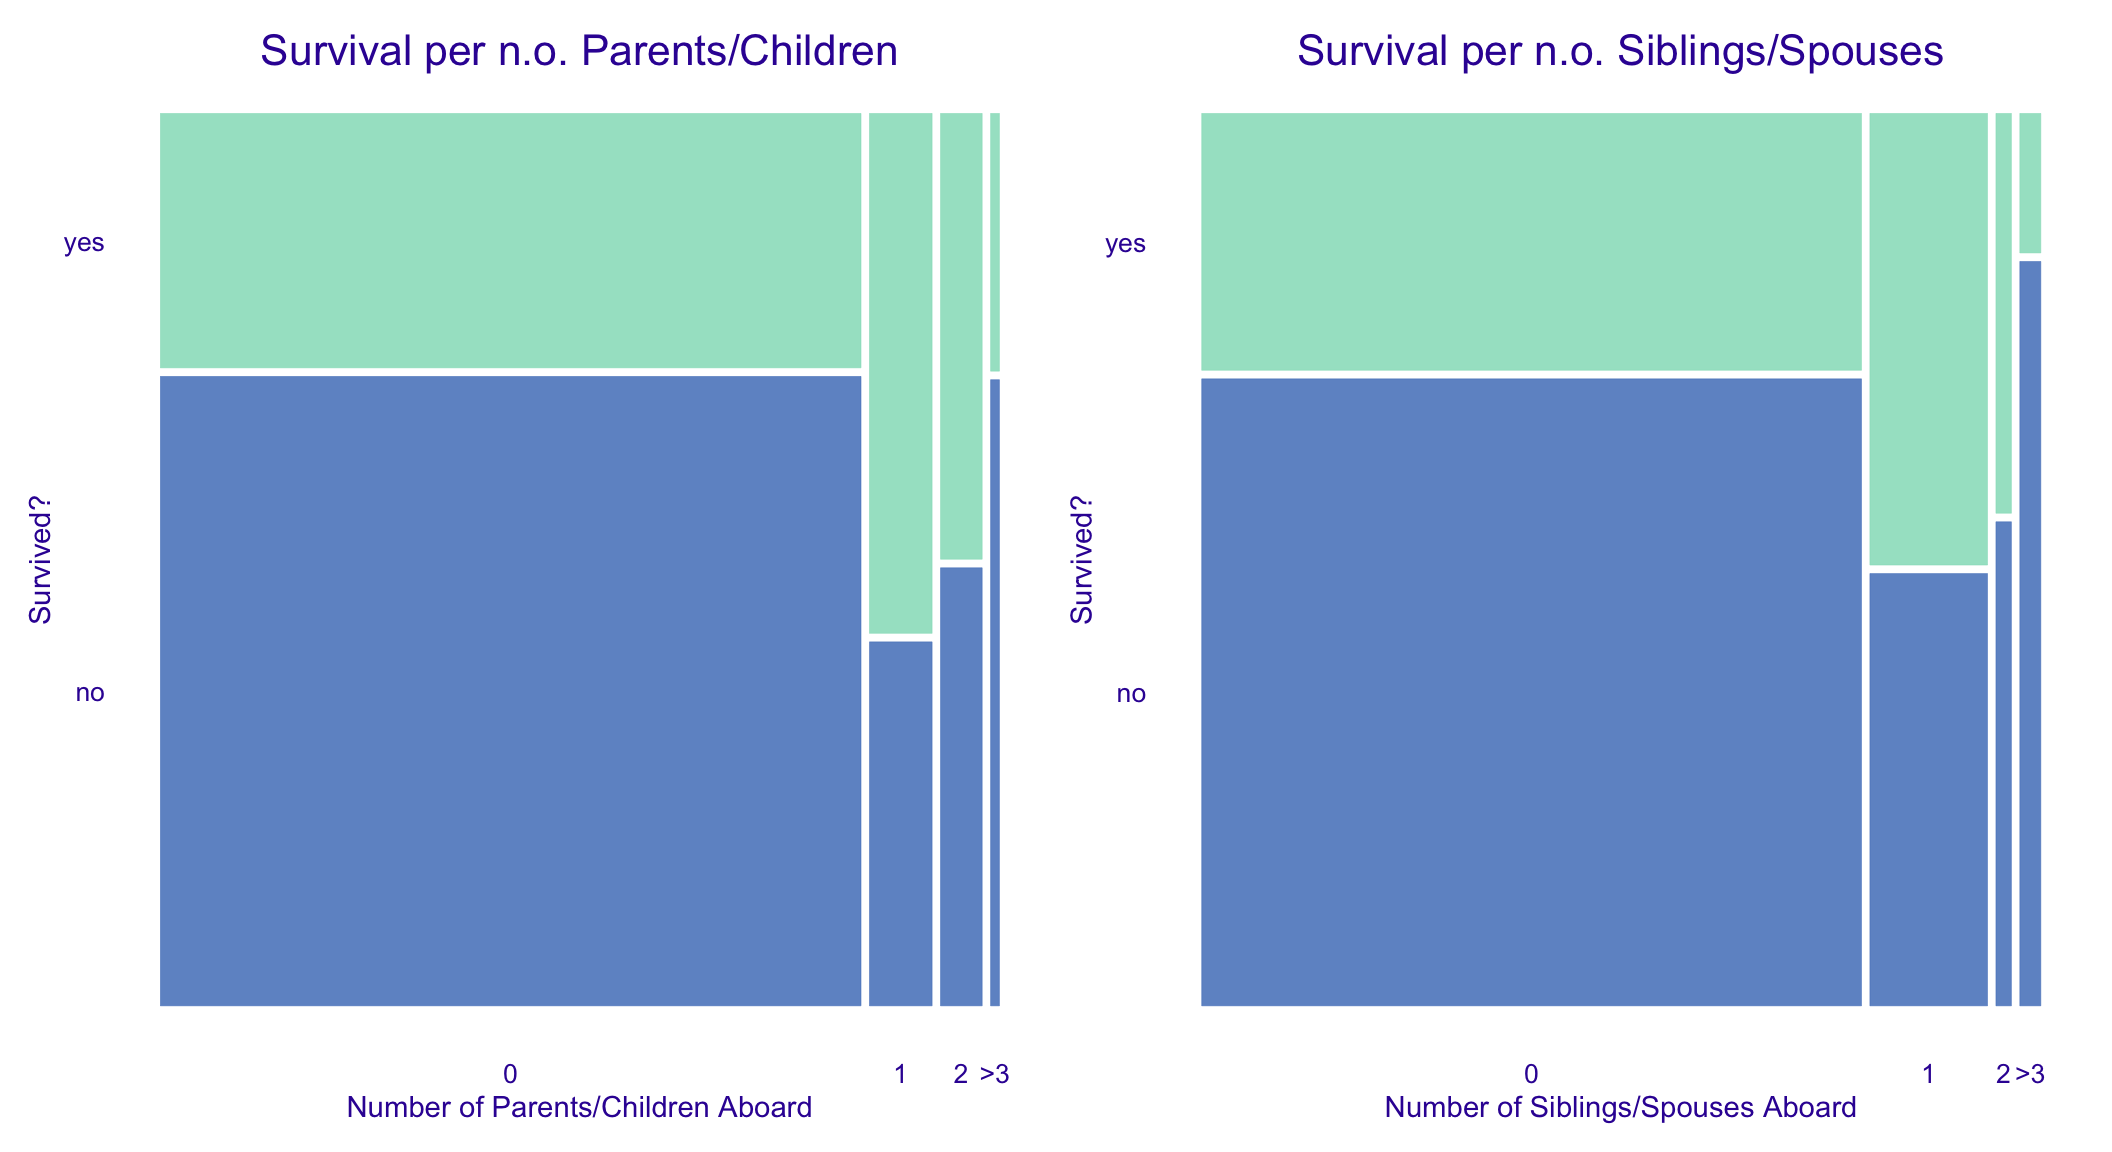
\includegraphics[width=0.7\linewidth]{PM_VEE_files/figure-latex/titanicExplorationParch-1} 

}

\caption{Survival according to the number of parents/children in the Titanic data.}\label{fig:titanicExplorationParch}
\end{figure}

\begin{figure}

{\centering 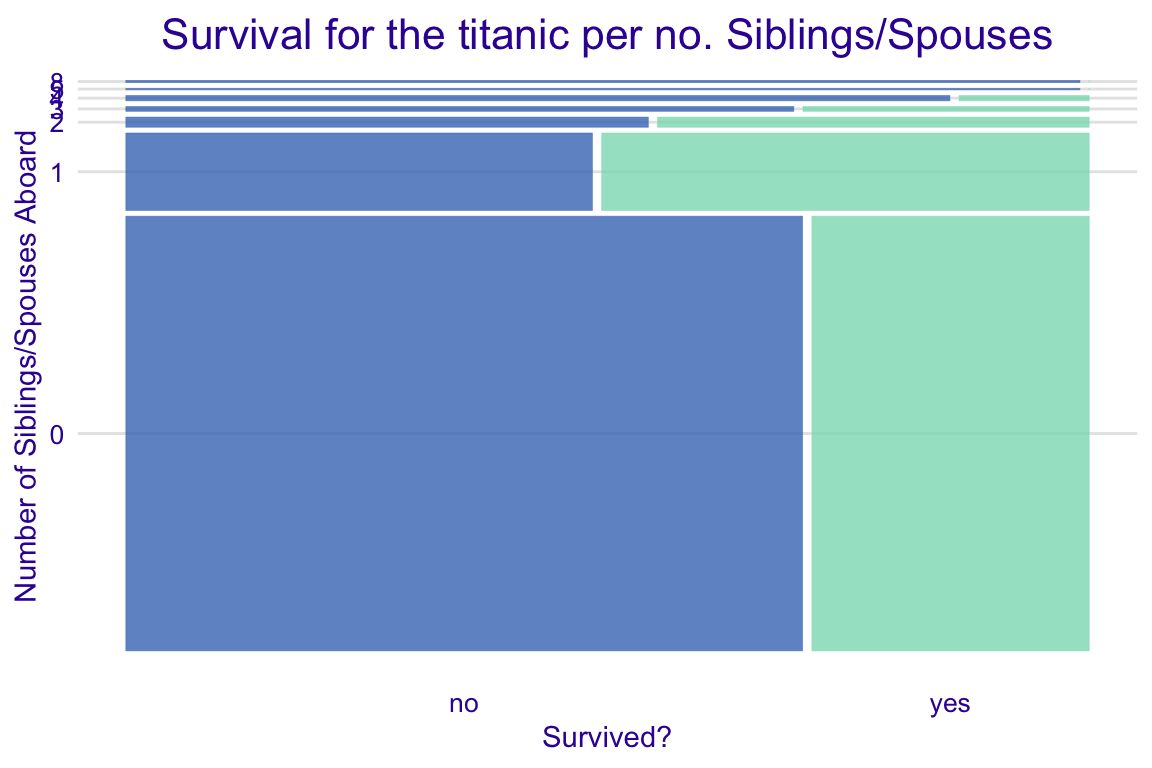
\includegraphics[width=0.7\linewidth]{PM_VEE_files/figure-latex/titanicExplorationSibsp-1} 

}

\caption{Survival according to the number of siblings/spouses in the Titanic data.}\label{fig:titanicExplorationSibsp}
\end{figure}
\begin{figure}

{\centering 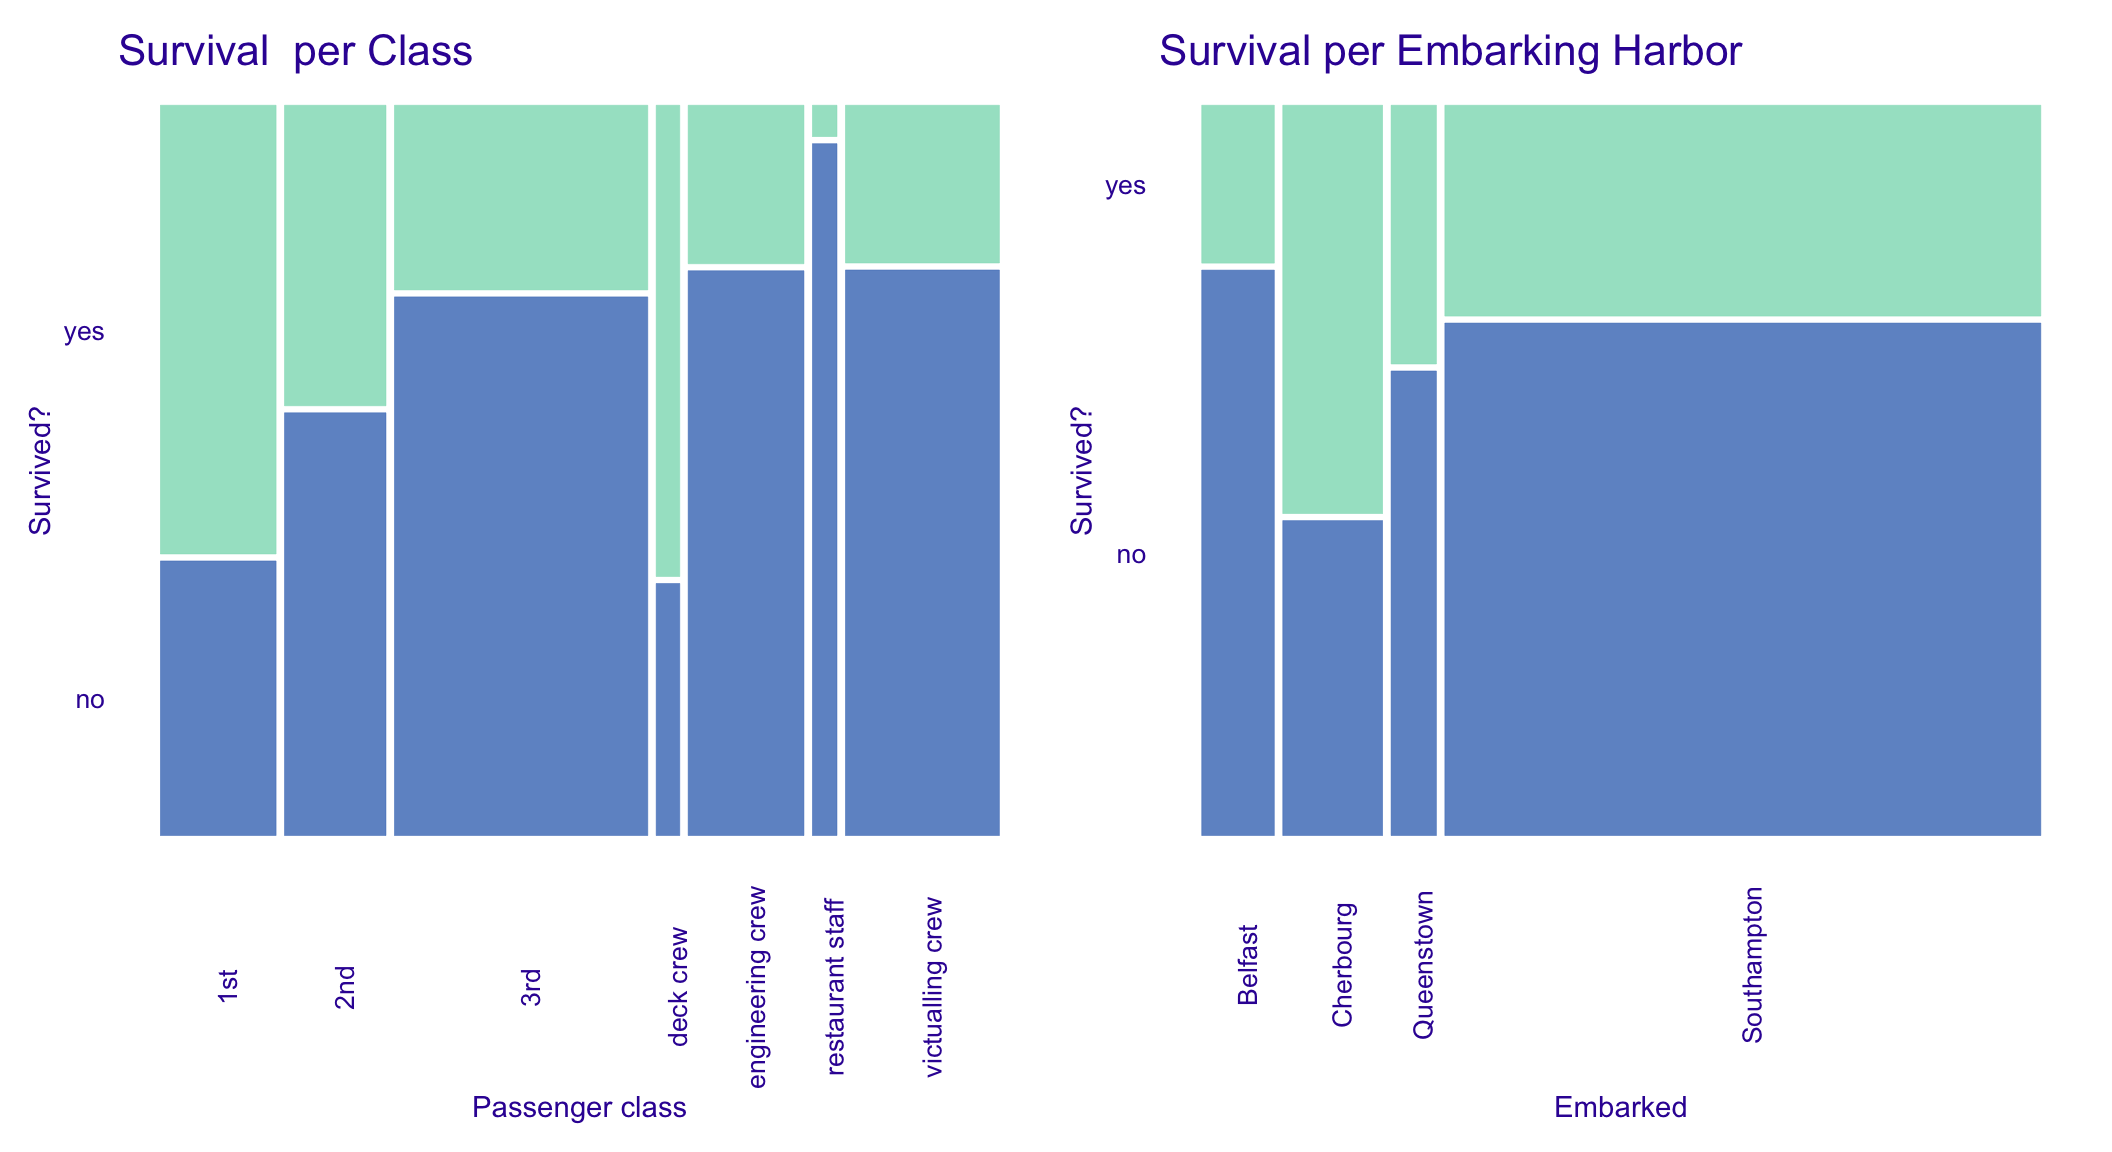
\includegraphics[width=0.7\linewidth]{PM_VEE_files/figure-latex/titanicExplorationClass-1} 

}

\caption{Survival according to the class in the Titanic data.}\label{fig:titanicExplorationClass}
\end{figure}

\begin{figure}

{\centering 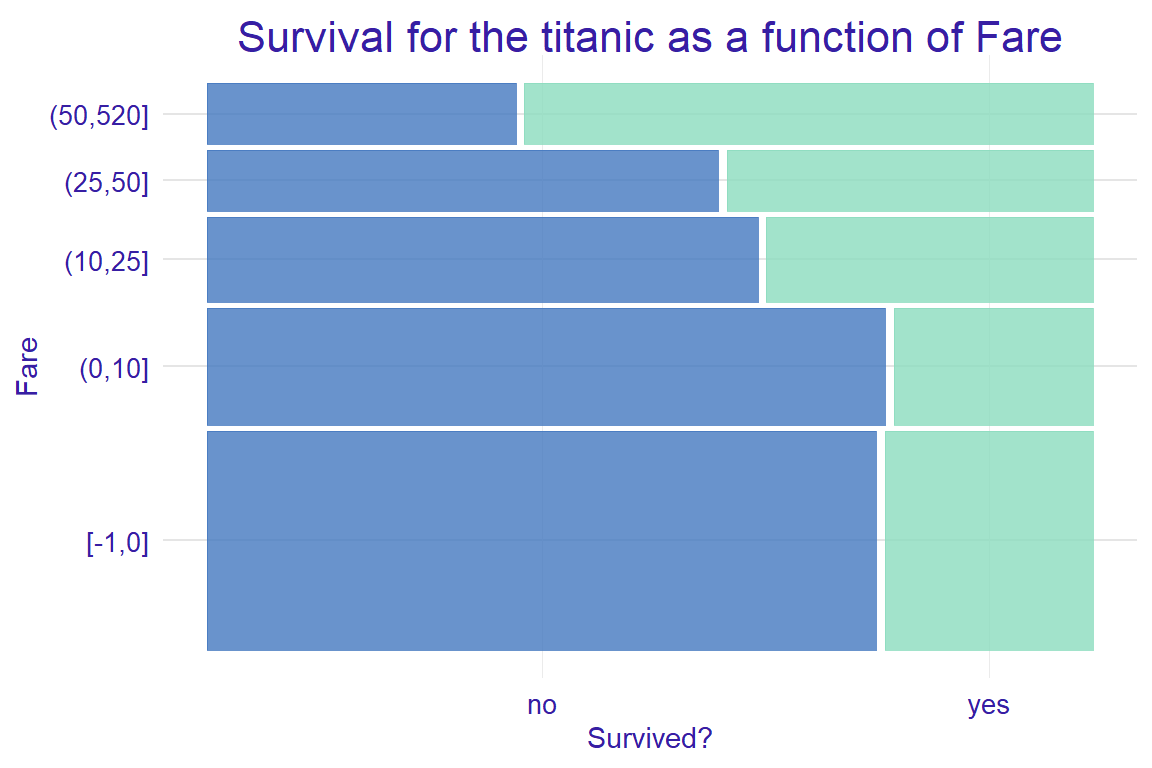
\includegraphics[width=0.7\linewidth]{PM_VEE_files/figure-latex/titanicExplorationFare-1} 

}

\caption{Survival according to fare in the Titanic data.}\label{fig:titanicExplorationFare}
\end{figure}

\begin{figure}

{\centering 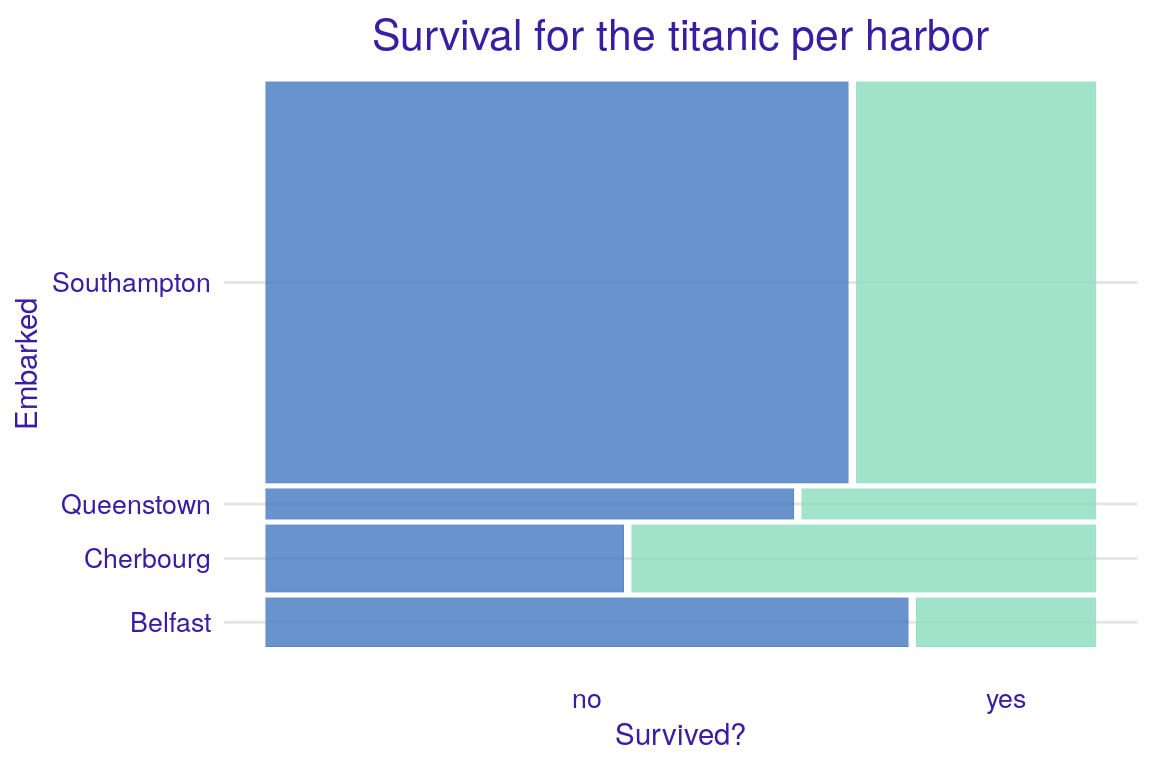
\includegraphics[width=0.7\linewidth]{PM_VEE_files/figure-latex/titanicExplorationEmbarked-1} 

}

\caption{Survival according to the port of embarking in the Titanic data.}\label{fig:titanicExplorationEmbarked}
\end{figure}

\begin{figure}

{\centering 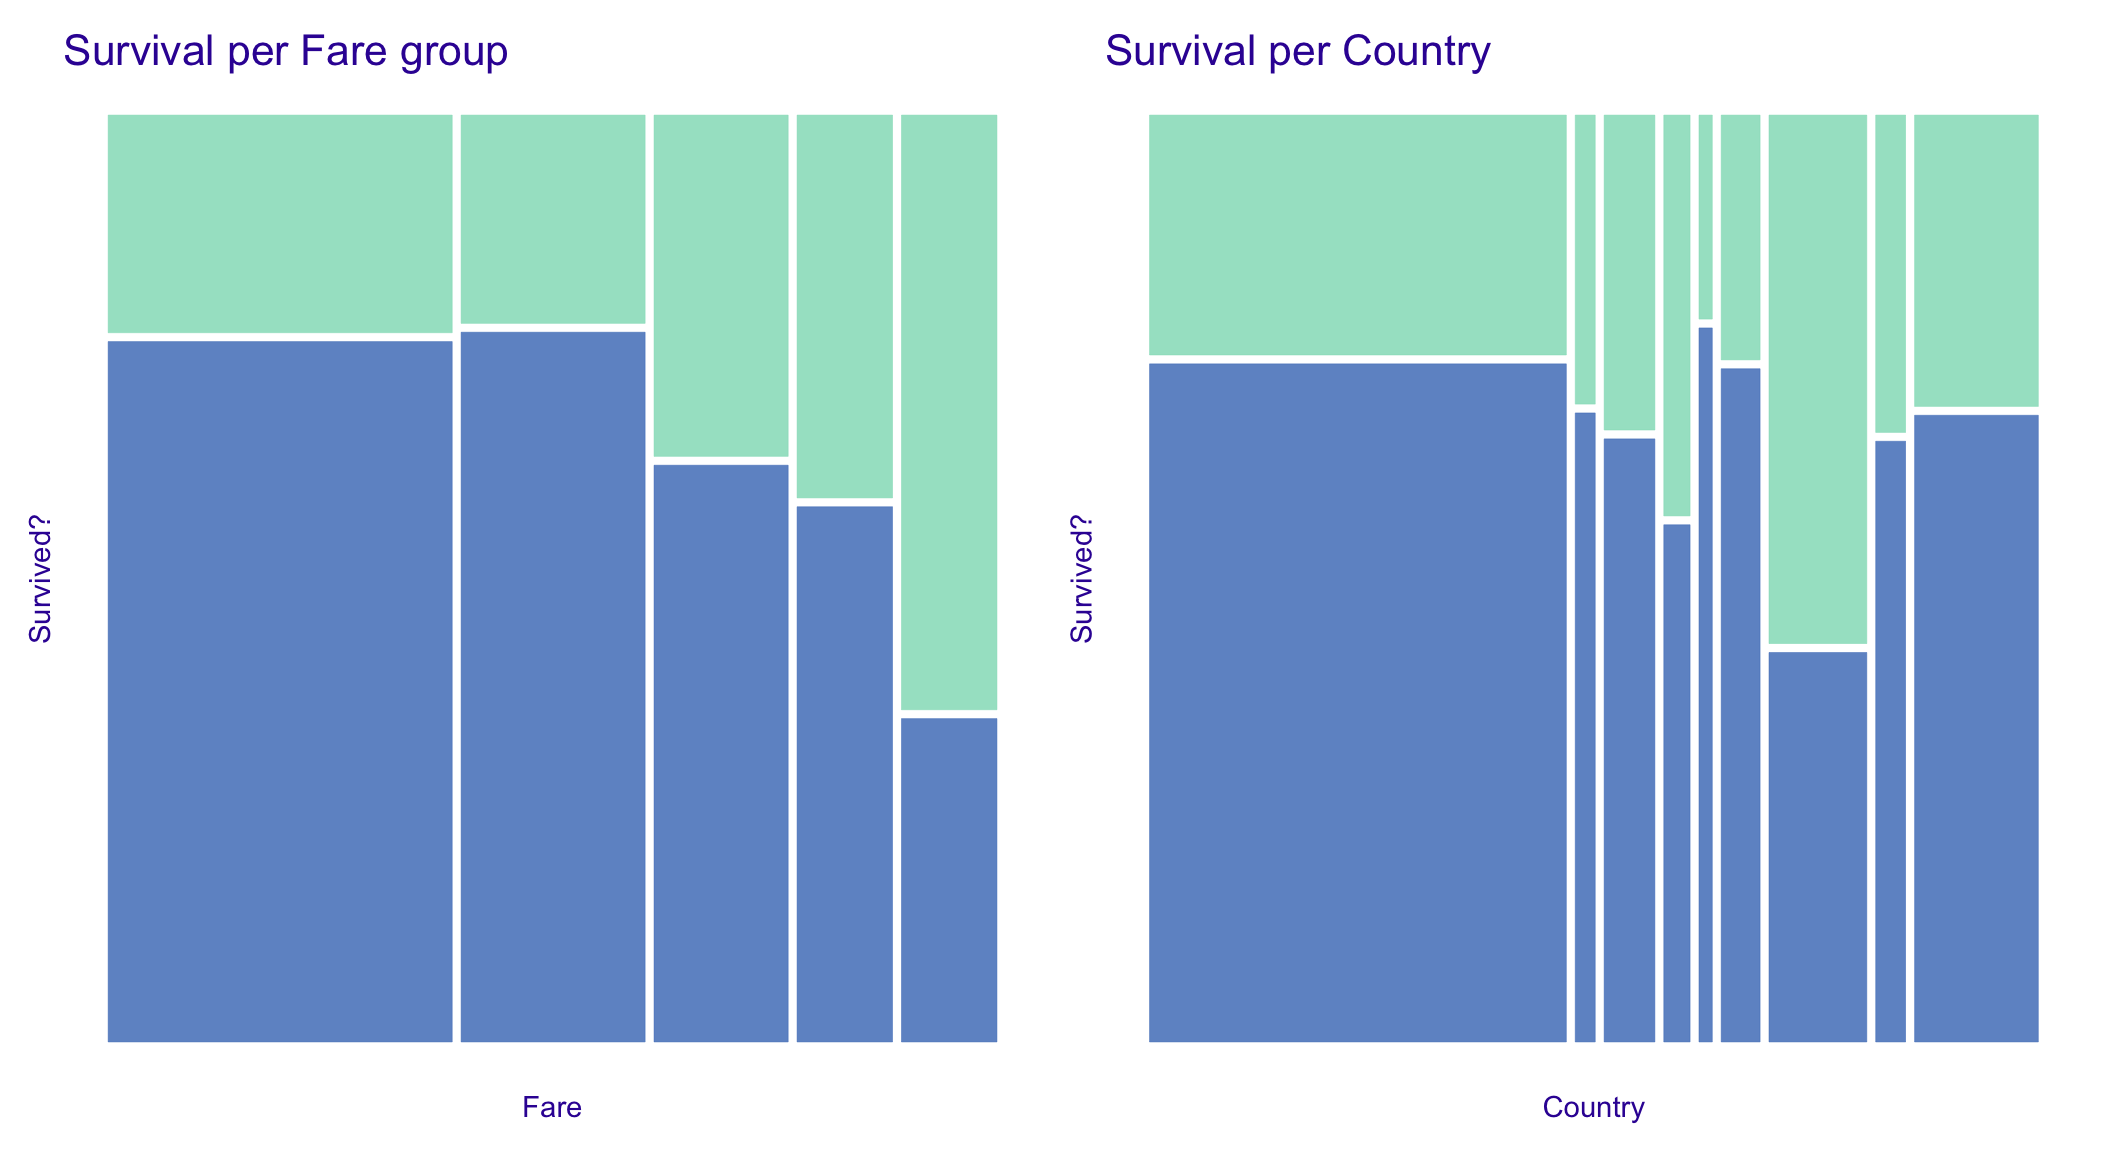
\includegraphics[width=0.7\linewidth]{PM_VEE_files/figure-latex/titanicExplorationCountry-1} 

}

\caption{Survival according to country in the Titanic data.}\label{fig:titanicExplorationCountry}
\end{figure}

\hypertarget{model-titanic-lmr}{%
\subsubsection{Logistic regression}\label{model-titanic-lmr}}

The dependent variable of interest, \emph{survival}, is binary. Thus, a natural choice to build a predictive model is logistic regression. We do not consider country as an explanatory variable. As there is no reason to expect a linear relationship between age and odds of survival, we use linear tail-restricted cubic splines, available in the \texttt{rcs()} function of the \texttt{rms} package \citep{rms}, to model the effect of age. We also do not expect linear relation for the \texttt{fare} variable, but because of it's skewness, we do not use splines for this variable. The results of the model are stored in model-object \texttt{titanic\_lmr\_v6}, which will be used in subsequent chapters.

\begin{Shaded}
\begin{Highlighting}[]
\KeywordTok{library}\NormalTok{(}\StringTok{"rms"}\NormalTok{)}
\KeywordTok{set.seed}\NormalTok{(}\DecValTok{1313}\NormalTok{)}
\NormalTok{titanic_lmr_v6 <-}\StringTok{ }\KeywordTok{lrm}\NormalTok{(survived }\OperatorTok{==}\StringTok{ "yes"} \OperatorTok{~}\StringTok{ }\NormalTok{gender }\OperatorTok{+}\StringTok{ }\KeywordTok{rcs}\NormalTok{(age) }\OperatorTok{+}\StringTok{ }\NormalTok{class }\OperatorTok{+}\StringTok{ }\NormalTok{sibsp }\OperatorTok{+}
\StringTok{                   }\NormalTok{parch }\OperatorTok{+}\StringTok{ }\NormalTok{fare }\OperatorTok{+}\StringTok{ }\NormalTok{embarked, titanic)}
\NormalTok{titanic_lmr_v6}
\end{Highlighting}
\end{Shaded}

\begin{verbatim}
## Logistic Regression Model
##  
##  lrm(formula = survived == "yes" ~ gender + rcs(age) + class + 
##      sibsp + parch + fare + embarked, data = titanic)
##  
##                         Model Likelihood     Discrimination    Rank Discrim.    
##                            Ratio Test           Indexes           Indexes       
##  Obs           2207    LR chi2     752.06    R2       0.404    C       0.817    
##   FALSE        1496    d.f.            17    g        1.647    Dxy     0.635    
##   TRUE          711    Pr(> chi2) <0.0001    gr       5.191    gamma   0.636    
##  max |deriv| 0.0001                          gp       0.282    tau-a   0.277    
##                                              Brier    0.146                     
##  
##                         Coef    S.E.   Wald Z Pr(>|Z|)
##  Intercept               4.5746 0.5480   8.35 <0.0001 
##  gender=male            -2.7687 0.1586 -17.45 <0.0001 
##  age                    -0.1180 0.0221  -5.35 <0.0001 
##  age'                    0.6313 0.1628   3.88 0.0001  
##  age''                  -2.6583 0.7840  -3.39 0.0007  
##  age'''                  2.8977 1.0130   2.86 0.0042  
##  class=2nd              -1.1390 0.2501  -4.56 <0.0001 
##  class=3rd              -2.0627 0.2490  -8.28 <0.0001 
##  class=deck crew         1.0672 0.3498   3.05 0.0023  
##  class=engineering crew -0.9702 0.2648  -3.66 0.0002  
##  class=restaurant staff -3.1712 0.6583  -4.82 <0.0001 
##  class=victualling crew -1.0877 0.2596  -4.19 <0.0001 
##  sibsp                  -0.4504 0.1006  -4.48 <0.0001 
##  parch                  -0.0871 0.0987  -0.88 0.3776  
##  fare                    0.0014 0.0020   0.70 0.4842  
##  embarked=Cherbourg      0.7881 0.2836   2.78 0.0055  
##  embarked=Queenstown     0.2745 0.3409   0.80 0.4208  
##  embarked=Southampton    0.2343 0.2119   1.11 0.2689  
## 
\end{verbatim}

\hypertarget{model-titanic-rf}{%
\subsubsection{Random forest}\label{model-titanic-rf}}

As an alternative to a logistic regression model, we consider a random forest model. Random forest is known for good predictive performance, is able to grasp low-level variable interactions, and is quite stable \citep{randomForestBreiman}. To fit the model, we apply the \texttt{randomForest()} function, with default settings, from the package with the same name \citep{randomForestRNews}.

In the first instance, we fit a model with the same set of explanatory variables as the logistic regression model. The results of the model are stored in model-object \texttt{titanic\_rf\_v6}.

\begin{Shaded}
\begin{Highlighting}[]
\KeywordTok{library}\NormalTok{(}\StringTok{"randomForest"}\NormalTok{)}
\KeywordTok{set.seed}\NormalTok{(}\DecValTok{1313}\NormalTok{)}
\NormalTok{titanic_rf_v6 <-}\StringTok{ }\KeywordTok{randomForest}\NormalTok{(survived }\OperatorTok{~}\StringTok{ }\NormalTok{class }\OperatorTok{+}\StringTok{ }\NormalTok{gender }\OperatorTok{+}\StringTok{ }\NormalTok{age }\OperatorTok{+}\StringTok{ }\NormalTok{sibsp }\OperatorTok{+}\StringTok{ }\NormalTok{parch }\OperatorTok{+}\StringTok{ }\NormalTok{fare }\OperatorTok{+}\StringTok{ }\NormalTok{embarked, }
                           \DataTypeTok{data =}\NormalTok{ titanic)}
\NormalTok{titanic_rf_v6}
\end{Highlighting}
\end{Shaded}

\begin{verbatim}
## 
## Call:
##  randomForest(formula = survived ~ class + gender + age + sibsp +      parch + fare + embarked, data = titanic) 
##                Type of random forest: classification
##                      Number of trees: 500
## No. of variables tried at each split: 2
## 
##         OOB estimate of  error rate: 18.62%
## Confusion matrix:
##       no yes class.error
## no  1393 103  0.06885027
## yes  308 403  0.43319269
\end{verbatim}

For comparison purposes, we also consider a model with only three explanatory variables: \emph{class}, \emph{gender}, and \emph{age}. The results of the model are stored in model-object \texttt{titanic\_rf\_v3}.

\begin{Shaded}
\begin{Highlighting}[]
\NormalTok{titanic_rf_v3 <-}\StringTok{ }\KeywordTok{randomForest}\NormalTok{(survived }\OperatorTok{~}\StringTok{ }\NormalTok{class }\OperatorTok{+}\StringTok{ }\NormalTok{gender }\OperatorTok{+}\StringTok{ }\NormalTok{age, }\DataTypeTok{data =}\NormalTok{ titanic)}
\NormalTok{titanic_rf_v3}
\end{Highlighting}
\end{Shaded}

\begin{verbatim}
## 
## Call:
##  randomForest(formula = survived ~ class + gender + age, data = titanic) 
##                Type of random forest: classification
##                      Number of trees: 500
## No. of variables tried at each split: 1
## 
##         OOB estimate of  error rate: 21.02%
## Confusion matrix:
##       no yes class.error
## no  1367 129  0.08622995
## yes  335 376  0.47116737
\end{verbatim}

\hypertarget{model-titanic-gbm}{%
\subsubsection{Gradient boosting}\label{model-titanic-gbm}}

Finally, we consider the gradient-boosting model. \citep{Friedman00greedyfunction} The model is known for being able to accomodate higher-order interactions between variables. We use the same set of explanatory variables as for the logistic regression model. To fit the gradient-boosting model, we use function \texttt{gbm()} from the \texttt{gbm} package \citep{gbm}. The results of the model are stored in model-object \texttt{titanic\_gbm\_v6}.

\begin{Shaded}
\begin{Highlighting}[]
\KeywordTok{library}\NormalTok{(}\StringTok{"gbm"}\NormalTok{)}
\KeywordTok{set.seed}\NormalTok{(}\DecValTok{1313}\NormalTok{)}
\NormalTok{titanic_gbm_v6 <-}\StringTok{ }\KeywordTok{gbm}\NormalTok{(survived }\OperatorTok{==}\StringTok{ "yes"} \OperatorTok{~}\StringTok{ }\NormalTok{class }\OperatorTok{+}\StringTok{ }\NormalTok{gender }\OperatorTok{+}\StringTok{ }\NormalTok{age }\OperatorTok{+}\StringTok{ }\NormalTok{sibsp }\OperatorTok{+}\StringTok{ }\NormalTok{parch }\OperatorTok{+}\StringTok{ }\NormalTok{fare }\OperatorTok{+}\StringTok{ }\NormalTok{embarked, }
                      \DataTypeTok{data =}\NormalTok{ titanic, }\DataTypeTok{n.trees =} \DecValTok{15000}\NormalTok{)}
\end{Highlighting}
\end{Shaded}

\begin{verbatim}
## Distribution not specified, assuming bernoulli ...
\end{verbatim}

\begin{Shaded}
\begin{Highlighting}[]
\NormalTok{titanic_gbm_v6}
\end{Highlighting}
\end{Shaded}

\begin{verbatim}
## gbm(formula = survived == "yes" ~ class + gender + age + sibsp + 
##     parch + fare + embarked, data = titanic, n.trees = 15000)
## A gradient boosted model with bernoulli loss function.
## 15000 iterations were performed.
## There were 7 predictors of which 7 had non-zero influence.
\end{verbatim}

\hypertarget{predictions-titanic}{%
\subsubsection{Model predictions}\label{predictions-titanic}}

Let us now compare predictions that are obtained from the three different models. In particular, we will compute the predicted probability of survival for an 8-year-old boy who embarked in Belfast and travelled in the 1-st class with no parents nor siblings and with a ticket costing 72 pounds.

First, we create a data frame \texttt{johny\_d} that contains the data describing the passenger.

\begin{Shaded}
\begin{Highlighting}[]
\NormalTok{johny_d <-}\StringTok{ }\KeywordTok{data.frame}\NormalTok{(}
            \DataTypeTok{class =} \KeywordTok{factor}\NormalTok{(}\StringTok{"1st"}\NormalTok{, }\DataTypeTok{levels =} \KeywordTok{c}\NormalTok{(}\StringTok{"1st"}\NormalTok{, }\StringTok{"2nd"}\NormalTok{, }\StringTok{"3rd"}\NormalTok{, }\StringTok{"deck crew"}\NormalTok{, }\StringTok{"engineering crew"}\NormalTok{, }\StringTok{"restaurant staff"}\NormalTok{, }\StringTok{"victualling crew"}\NormalTok{)),}
            \DataTypeTok{gender =} \KeywordTok{factor}\NormalTok{(}\StringTok{"male"}\NormalTok{, }\DataTypeTok{levels =} \KeywordTok{c}\NormalTok{(}\StringTok{"female"}\NormalTok{, }\StringTok{"male"}\NormalTok{)),}
            \DataTypeTok{age =} \DecValTok{8}\NormalTok{,}
            \DataTypeTok{sibsp =} \DecValTok{0}\NormalTok{,}
            \DataTypeTok{parch =} \DecValTok{0}\NormalTok{,}
            \DataTypeTok{fare =} \DecValTok{72}\NormalTok{,}
            \DataTypeTok{embarked =} \KeywordTok{factor}\NormalTok{(}\StringTok{"Southampton"}\NormalTok{, }\DataTypeTok{levels =} \KeywordTok{c}\NormalTok{(}\StringTok{"Belfast"}\NormalTok{,}\StringTok{"Cherbourg"}\NormalTok{,}\StringTok{"Queenstown"}\NormalTok{,}\StringTok{"Southampton"}\NormalTok{))}
\NormalTok{)}
\end{Highlighting}
\end{Shaded}

Subsequently, we use the generic function \texttt{predict()} to get the predicted probability of survival for the logistic regression model.

\begin{Shaded}
\begin{Highlighting}[]
\NormalTok{(pred_lmr <-}\StringTok{ }\KeywordTok{predict}\NormalTok{(titanic_lmr_v6, johny_d, }\DataTypeTok{type =} \StringTok{"fitted"}\NormalTok{))}
\end{Highlighting}
\end{Shaded}

\begin{verbatim}
##         1 
## 0.7677036
\end{verbatim}

The predicted probability is equal to 0.77.

We do the same for the random forest and gradient boosting models.

\begin{Shaded}
\begin{Highlighting}[]
\NormalTok{(pred_rf <-}\StringTok{ }\KeywordTok{predict}\NormalTok{(titanic_rf_v6, johny_d, }\DataTypeTok{type =} \StringTok{"prob"}\NormalTok{))}
\end{Highlighting}
\end{Shaded}

\begin{verbatim}
##      no   yes
## 1 0.578 0.422
## attr(,"class")
## [1] "matrix" "votes"
\end{verbatim}

\begin{Shaded}
\begin{Highlighting}[]
\NormalTok{(pred_gbm <-}\StringTok{ }\KeywordTok{predict}\NormalTok{(titanic_gbm_v6, johny_d, }\DataTypeTok{type =} \StringTok{"response"}\NormalTok{, }\DataTypeTok{n.trees =} \DecValTok{15000}\NormalTok{))}
\end{Highlighting}
\end{Shaded}

\begin{verbatim}
## [1] 0.6632574
\end{verbatim}

As a result, we obtain the predicted probabilities of 0.42 and 0.66, respectively.

The models lead to different probabilities. Thus, it might be of interest to understand the reason for the differences, as it could help us to decide which of the predictions we might want to trust.

Note that for some examples we will use another observation (instance) with lower chances of survival. Let's call this passenger Henry.

\begin{Shaded}
\begin{Highlighting}[]
\NormalTok{henry <-}\StringTok{ }\KeywordTok{data.frame}\NormalTok{(}
            \DataTypeTok{class =} \KeywordTok{factor}\NormalTok{(}\StringTok{"1st"}\NormalTok{, }\DataTypeTok{levels =} \KeywordTok{c}\NormalTok{(}\StringTok{"1st"}\NormalTok{, }\StringTok{"2nd"}\NormalTok{, }\StringTok{"3rd"}\NormalTok{, }\StringTok{"deck crew"}\NormalTok{, }\StringTok{"engineering crew"}\NormalTok{, }\StringTok{"restaurant staff"}\NormalTok{, }\StringTok{"victualling crew"}\NormalTok{)),}
            \DataTypeTok{gender =} \KeywordTok{factor}\NormalTok{(}\StringTok{"male"}\NormalTok{, }\DataTypeTok{levels =} \KeywordTok{c}\NormalTok{(}\StringTok{"female"}\NormalTok{, }\StringTok{"male"}\NormalTok{)),}
            \DataTypeTok{age =} \DecValTok{47}\NormalTok{,}
            \DataTypeTok{sibsp =} \DecValTok{0}\NormalTok{,}
            \DataTypeTok{parch =} \DecValTok{0}\NormalTok{,}
            \DataTypeTok{fare =} \DecValTok{25}\NormalTok{,}
            \DataTypeTok{embarked =} \KeywordTok{factor}\NormalTok{(}\StringTok{"Cherbourg"}\NormalTok{, }\DataTypeTok{levels =} \KeywordTok{c}\NormalTok{(}\StringTok{"Belfast"}\NormalTok{,}\StringTok{"Cherbourg"}\NormalTok{,}\StringTok{"Queenstown"}\NormalTok{,}\StringTok{"Southampton"}\NormalTok{))}
\NormalTok{)}
\KeywordTok{round}\NormalTok{(}\KeywordTok{predict}\NormalTok{(titanic_lmr_v6, henry, }\DataTypeTok{type =} \StringTok{"fitted"}\NormalTok{),}\DecValTok{2}\NormalTok{)}
\end{Highlighting}
\end{Shaded}

\begin{verbatim}
##    1 
## 0.43
\end{verbatim}

\begin{Shaded}
\begin{Highlighting}[]
\KeywordTok{round}\NormalTok{(}\KeywordTok{predict}\NormalTok{(titanic_rf_v6, henry, }\DataTypeTok{type =} \StringTok{"prob"}\NormalTok{)[}\DecValTok{1}\NormalTok{,}\DecValTok{2}\NormalTok{],}\DecValTok{2}\NormalTok{)}
\end{Highlighting}
\end{Shaded}

\begin{verbatim}
## [1] 0.25
\end{verbatim}

\begin{Shaded}
\begin{Highlighting}[]
\KeywordTok{round}\NormalTok{(}\KeywordTok{predict}\NormalTok{(titanic_gbm_v6, henry, }\DataTypeTok{type =} \StringTok{"response"}\NormalTok{, }\DataTypeTok{n.trees =} \DecValTok{15000}\NormalTok{),}\DecValTok{2}\NormalTok{)}
\end{Highlighting}
\end{Shaded}

\begin{verbatim}
## [1] 0.31
\end{verbatim}

\hypertarget{ExplainersTitanicRCode}{%
\subsubsection{Explainers}\label{ExplainersTitanicRCode}}

Model-objects created with different libraries may have different internal structures. Thus, first, we have got to create a wrapper around the model. Toward this end, we use the \texttt{explain()} function from the \texttt{DALEX} package \citep{DALEX}. The function requires five arguments:

\begin{itemize}
\tightlist
\item
  \texttt{model}, a model-object;
\item
  \texttt{data}, a validation data frame;
\item
  \texttt{y}, observed values of the dependent variable for the validation data;
\item
  \texttt{predict\_function}, a function that returns prediction scores; if not specified, then a default \texttt{predict()} function is used;
\item
  \texttt{label}, a function that returns prediction scores; if not specified, then it is extracted from the \texttt{class(model)}.
  In the example below we create explainers for the logistic regression, random forest, and gradient boosting models created for the Titanic data.
\end{itemize}

Each explainer wraps all elements needed to create a model explanation, i.e., a suitable \texttt{predict()} function, validation data set, and the model object. Thus, in subsequent chapters we will use the explainers instead of the model objects to keep code snippets more concise.

\begin{Shaded}
\begin{Highlighting}[]
\NormalTok{explain_titanic_lmr_v6 <-}\StringTok{ }\KeywordTok{explain}\NormalTok{(}\DataTypeTok{model =}\NormalTok{ titanic_lmr_v6, }
                                 \DataTypeTok{data =}\NormalTok{ titanic[, }\DecValTok{-9}\NormalTok{],}
                                 \DataTypeTok{y =}\NormalTok{ titanic}\OperatorTok{$}\NormalTok{survived }\OperatorTok{==}\StringTok{ "yes"}\NormalTok{, }
                                 \DataTypeTok{predict_function =} \ControlFlowTok{function}\NormalTok{(m, x) }\KeywordTok{predict}\NormalTok{(m, x, }\DataTypeTok{type =} \StringTok{"fitted"}\NormalTok{),}
                                 \DataTypeTok{label =} \StringTok{"Logistic Regression v6"}\NormalTok{)}
\NormalTok{explain_titanic_rf_v6 <-}\StringTok{ }\KeywordTok{explain}\NormalTok{(}\DataTypeTok{model =}\NormalTok{ titanic_rf_v6, }
                                 \DataTypeTok{data =}\NormalTok{ titanic[, }\DecValTok{-9}\NormalTok{],}
                                 \DataTypeTok{y =}\NormalTok{ titanic}\OperatorTok{$}\NormalTok{survived }\OperatorTok{==}\StringTok{ "yes"}\NormalTok{, }
                                 \DataTypeTok{label =} \StringTok{"Random Forest v6"}\NormalTok{)}
\NormalTok{explain_titanic_rf_v3 <-}\StringTok{ }\KeywordTok{explain}\NormalTok{(}\DataTypeTok{model =}\NormalTok{ titanic_rf_v3, }
                                 \DataTypeTok{data =}\NormalTok{ titanic[, }\DecValTok{-9}\NormalTok{],}
                                 \DataTypeTok{y =}\NormalTok{ titanic}\OperatorTok{$}\NormalTok{survived }\OperatorTok{==}\StringTok{ "yes"}\NormalTok{, }
                                 \DataTypeTok{label =} \StringTok{"Random Forest v3"}\NormalTok{)}
\NormalTok{explain_titanic_gbm_v6 <-}\StringTok{ }\KeywordTok{explain}\NormalTok{(}\DataTypeTok{model =}\NormalTok{ titanic_gbm_v6, }
                                 \DataTypeTok{data =}\NormalTok{ titanic[, }\DecValTok{-9}\NormalTok{],}
                                 \DataTypeTok{y =}\NormalTok{ titanic}\OperatorTok{$}\NormalTok{survived }\OperatorTok{==}\StringTok{ "yes"}\NormalTok{, }
                                 \DataTypeTok{predict_function =} \ControlFlowTok{function}\NormalTok{(m, x) }\KeywordTok{predict}\NormalTok{(m, x, }\DataTypeTok{n.trees =} \DecValTok{100}\NormalTok{),}
                                 \DataTypeTok{label =} \StringTok{"Generalized Boosted Regression v6"}\NormalTok{)}
\end{Highlighting}
\end{Shaded}

\hypertarget{ListOfModelsTitanic}{%
\subsubsection{\texorpdfstring{List of objects for the \texttt{titanic} example}{List of objects for the titanic example}}\label{ListOfModelsTitanic}}

In the previous sections we have built several predictive models for the \texttt{titanic} data set. The models will be used in the rest of the book to illustrate the model explanation methods and tools.

For the ease of reference, we summarize the models in Table \ref{tab:archivistHooksOfModelsTitanic}. The binary model-objects can be downloaded by using the indicated \texttt{archivist} hooks \citep{archivist}. By calling a function specified in the last column of the table, one can recreate a selected model in a local R environment.

\begin{longtable}[]{@{}llll@{}}
\caption{\label{tab:archivistHooksOfModelsTitanic} Predictive models created for the \texttt{titanic} dataset.}\tabularnewline
\toprule
\begin{minipage}[b]{0.21\columnwidth}\raggedright
Model name\strut
\end{minipage} & \begin{minipage}[b]{0.25\columnwidth}\raggedright
Model generator\strut
\end{minipage} & \begin{minipage}[b]{0.18\columnwidth}\raggedright
Variables\strut
\end{minipage} & \begin{minipage}[b]{0.25\columnwidth}\raggedright
Archivist hooks\strut
\end{minipage}\tabularnewline
\midrule
\endfirsthead
\toprule
\begin{minipage}[b]{0.21\columnwidth}\raggedright
Model name\strut
\end{minipage} & \begin{minipage}[b]{0.25\columnwidth}\raggedright
Model generator\strut
\end{minipage} & \begin{minipage}[b]{0.18\columnwidth}\raggedright
Variables\strut
\end{minipage} & \begin{minipage}[b]{0.25\columnwidth}\raggedright
Archivist hooks\strut
\end{minipage}\tabularnewline
\midrule
\endhead
\begin{minipage}[t]{0.21\columnwidth}\raggedright
\texttt{titanic\_lmr\_v6}\strut
\end{minipage} & \begin{minipage}[t]{0.25\columnwidth}\raggedright
\texttt{rms::\ lmr} v.5.1.3\strut
\end{minipage} & \begin{minipage}[t]{0.18\columnwidth}\raggedright
gender, age, class, sibsp, parch, fare, embarked\strut
\end{minipage} & \begin{minipage}[t]{0.25\columnwidth}\raggedright
Get the model: \texttt{archivist::\ aread("pbiecek/models/ceb40")}. Get the explainer: \texttt{archivist::\ aread("pbiecek/models/51c50")}\strut
\end{minipage}\tabularnewline
\begin{minipage}[t]{0.21\columnwidth}\raggedright
\texttt{titanic\_rf\_v6}\strut
\end{minipage} & \begin{minipage}[t]{0.25\columnwidth}\raggedright
\texttt{randomForest::\ randomForest} v.4.6.14\strut
\end{minipage} & \begin{minipage}[t]{0.18\columnwidth}\raggedright
gender, age, class, sibsp, parch, fare, embarked\strut
\end{minipage} & \begin{minipage}[t]{0.25\columnwidth}\raggedright
Get the model: \texttt{archivist::\ aread("pbiecek/models/1f938")}. Get the explainer: \texttt{archivist::\ aread("pbiecek/models/42d51")}\strut
\end{minipage}\tabularnewline
\begin{minipage}[t]{0.21\columnwidth}\raggedright
\texttt{titanic\_rf\_v3}\strut
\end{minipage} & \begin{minipage}[t]{0.25\columnwidth}\raggedright
\texttt{randomForest::\ randomForest} v.4.6.14\strut
\end{minipage} & \begin{minipage}[t]{0.18\columnwidth}\raggedright
gender, age, class\strut
\end{minipage} & \begin{minipage}[t]{0.25\columnwidth}\raggedright
Get the model: \texttt{archivist::\ aread("pbiecek/models/855c1")}. Get the explainer: \texttt{archivist::\ aread("pbiecek/models/0e5d2")}\strut
\end{minipage}\tabularnewline
\begin{minipage}[t]{0.21\columnwidth}\raggedright
\texttt{titanic\_gbm\_v6}\strut
\end{minipage} & \begin{minipage}[t]{0.25\columnwidth}\raggedright
\texttt{gbm::\ gbm} v.2.1.5\strut
\end{minipage} & \begin{minipage}[t]{0.18\columnwidth}\raggedright
gender, age, class, sibsp, parch, fare, embarked\strut
\end{minipage} & \begin{minipage}[t]{0.25\columnwidth}\raggedright
Get the model: \texttt{archivist::\ aread("pbiecek/models/24e72")}. Get the explainer: \texttt{archivist::\ aread("pbiecek/models/3d514")}\strut
\end{minipage}\tabularnewline
\bottomrule
\end{longtable}

Table \ref{tab:archivistHooksOfDataFramesTitanic} summarizes the data frames that will be used in examples in the subsequent chapters.

\begin{longtable}[]{@{}llll@{}}
\caption{\label{tab:archivistHooksOfDataFramesTitanic} Data frames created for the \texttt{titanic} example.}\tabularnewline
\toprule
\begin{minipage}[b]{0.22\columnwidth}\raggedright
Description\strut
\end{minipage} & \begin{minipage}[b]{0.16\columnwidth}\raggedright
No.~rows\strut
\end{minipage} & \begin{minipage}[b]{0.19\columnwidth}\raggedright
Variables\strut
\end{minipage} & \begin{minipage}[b]{0.33\columnwidth}\raggedright
Link to this object\strut
\end{minipage}\tabularnewline
\midrule
\endfirsthead
\toprule
\begin{minipage}[b]{0.22\columnwidth}\raggedright
Description\strut
\end{minipage} & \begin{minipage}[b]{0.16\columnwidth}\raggedright
No.~rows\strut
\end{minipage} & \begin{minipage}[b]{0.19\columnwidth}\raggedright
Variables\strut
\end{minipage} & \begin{minipage}[b]{0.33\columnwidth}\raggedright
Link to this object\strut
\end{minipage}\tabularnewline
\midrule
\endhead
\begin{minipage}[t]{0.22\columnwidth}\raggedright
\texttt{titanic} dataset with imputed missing values\strut
\end{minipage} & \begin{minipage}[t]{0.16\columnwidth}\raggedright
2207\strut
\end{minipage} & \begin{minipage}[t]{0.19\columnwidth}\raggedright
gender, age, class, embarked, country, fare, sibsp, parch, survived\strut
\end{minipage} & \begin{minipage}[t]{0.33\columnwidth}\raggedright
\texttt{archivist::\ aread("pbiecek/models/27e5c")}\strut
\end{minipage}\tabularnewline
\begin{minipage}[t]{0.22\columnwidth}\raggedright
\texttt{johny\_d} 8-year-old boy that travelled in the 1st class without parents\strut
\end{minipage} & \begin{minipage}[t]{0.16\columnwidth}\raggedright
1\strut
\end{minipage} & \begin{minipage}[t]{0.19\columnwidth}\raggedright
class, gender, age, sibsp, parch, fare, embarked\strut
\end{minipage} & \begin{minipage}[t]{0.33\columnwidth}\raggedright
\texttt{archivist::\ aread("pbiecek/models/e3596")}\strut
\end{minipage}\tabularnewline
\begin{minipage}[t]{0.22\columnwidth}\raggedright
\texttt{henry} 47-year-old male passenger from the 1st class, paid 25 pounds and embarked at Cherbourg\strut
\end{minipage} & \begin{minipage}[t]{0.16\columnwidth}\raggedright
1\strut
\end{minipage} & \begin{minipage}[t]{0.19\columnwidth}\raggedright
class, gender, age, sibsp, parch, fare, embarked\strut
\end{minipage} & \begin{minipage}[t]{0.33\columnwidth}\raggedright
\texttt{archivist::\ aread("pbiecek/models/a6538")}\strut
\end{minipage}\tabularnewline
\bottomrule
\end{longtable}

\hypertarget{ApartmentDataset}{%
\subsection{Apartment prices}\label{ApartmentDataset}}

\begin{figure}
\centering
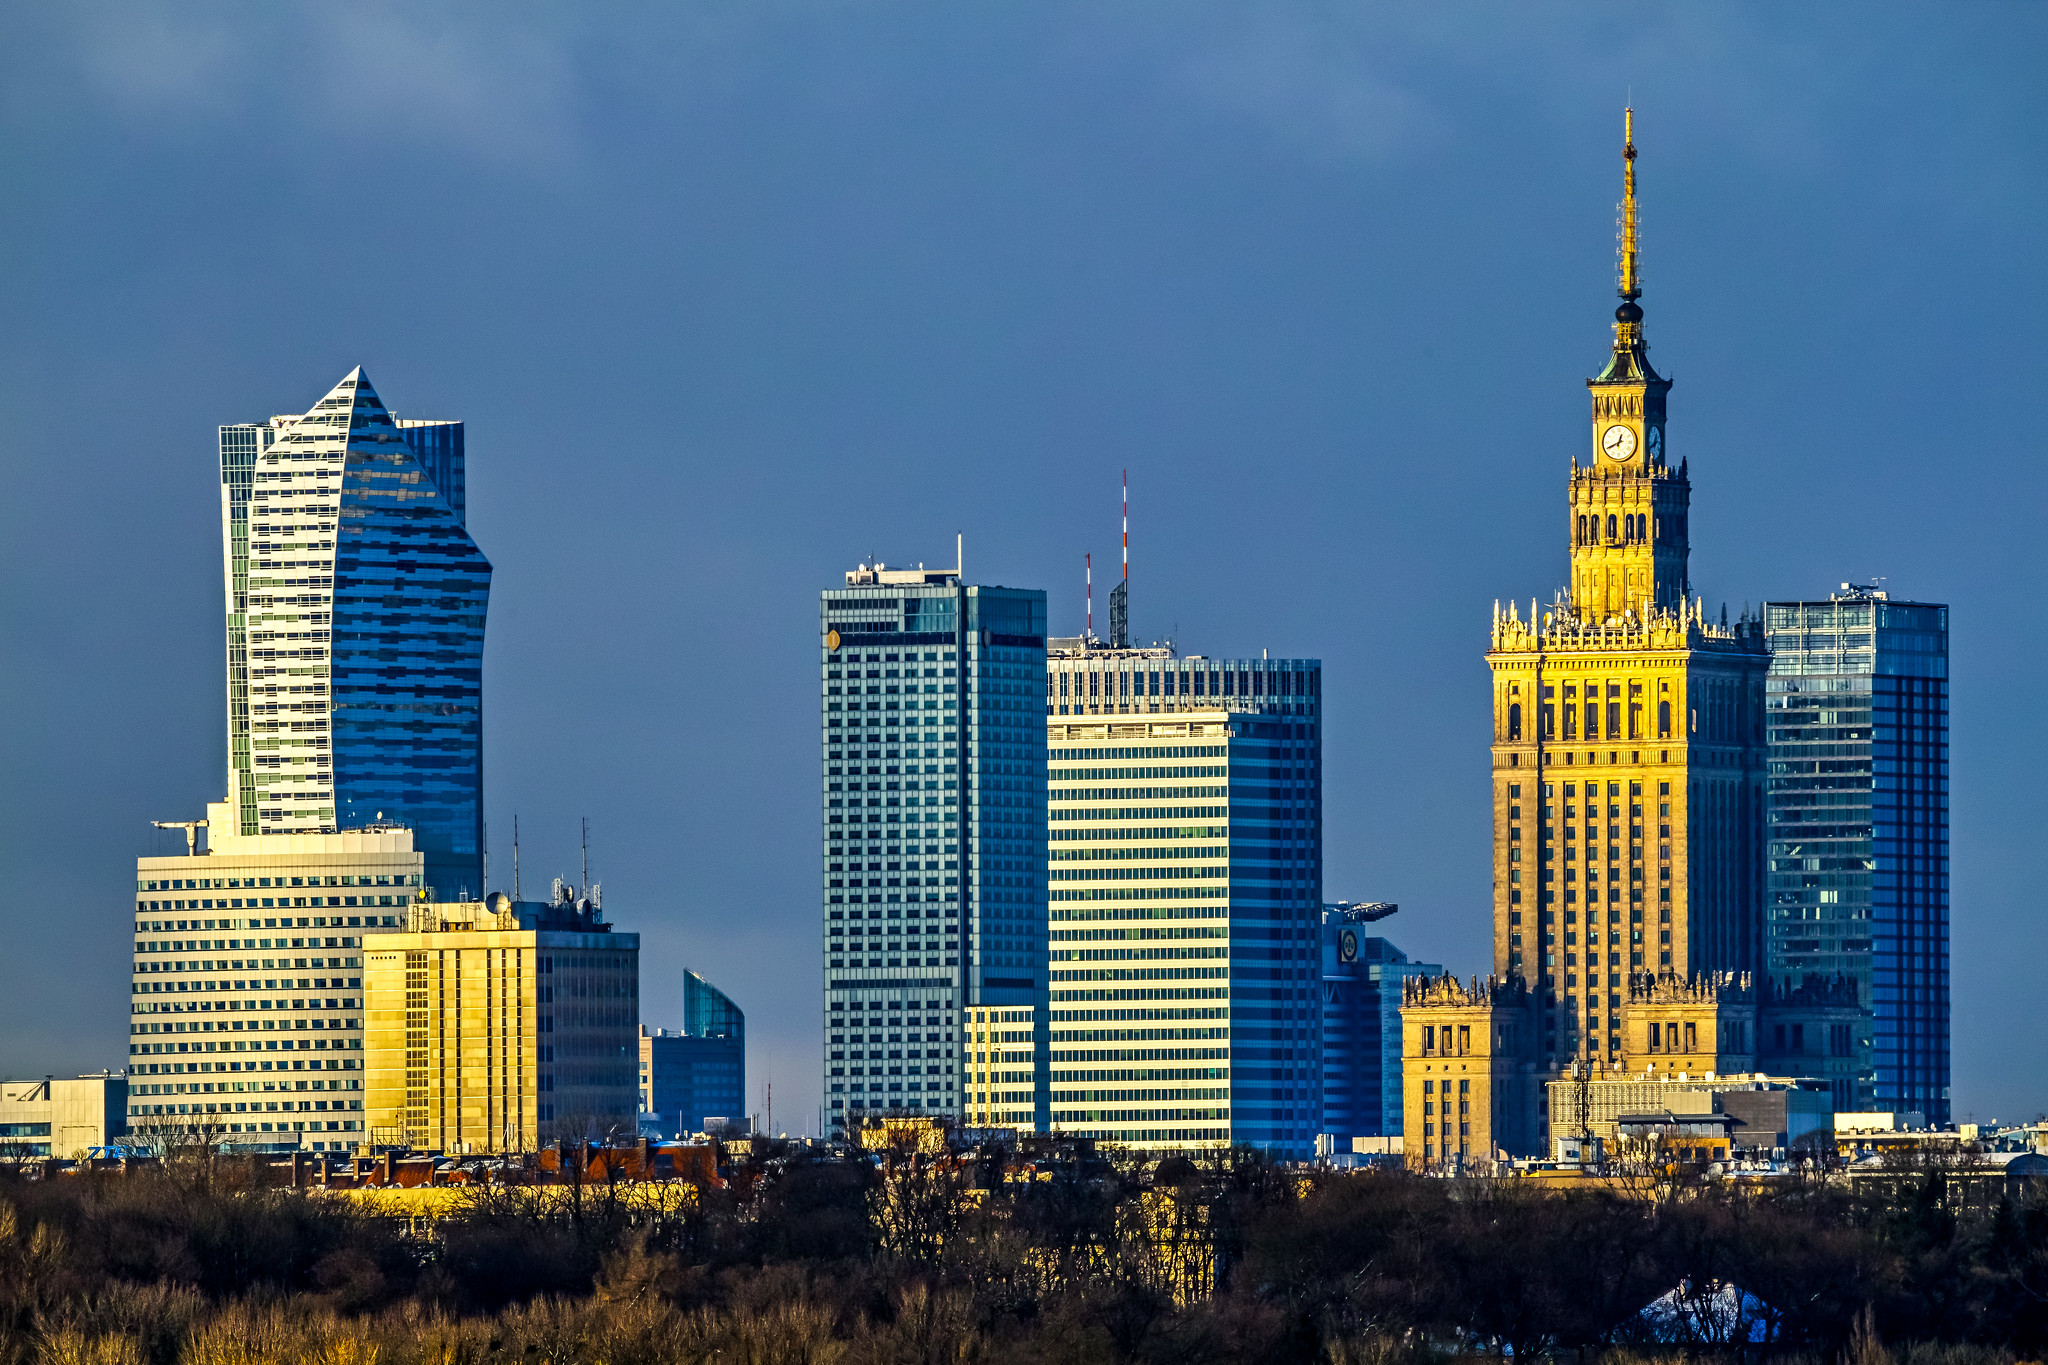
\includegraphics{figure/am1974_flicker.jpg}
\caption{Warsaw skyscrapers by Artur Malinowski Flicker}
\end{figure}

Predicting house prices is a common exercise used in machine-learning courses. Various datasets for house prices are available at websites like Kaggle (\url{https://www.kaggle.com}) or UCI Machine Learning Repository (\url{https://archive.ics.uci.edu}).

In this book, we will work with an interesting variant of this problem. The \texttt{apartments} dataset is an artificial dataset created to match key characteristics of real apartments in Warszawa, the capital of Poland. However, the dataset is created in a way that two very different models, namely linear regression and random forest, have almost exactly the same accuracy. The natural question is then: which model should we choose? We will show that the model-explanation tools provide important insight into the key model characteristics and are helpful in model selection.

The dataset is available in the \texttt{DALEX} package \citep{DALEX}. It contains 1000 observations (apartments) and six variables:

\begin{itemize}
\tightlist
\item
  \emph{m2.price}, apatments price per meter-squared (in EUR), a numerical variable;
\item
  \emph{construction.year}, the year of construction of the block of flats in which the apartment is located, a numerical variable;
\item
  \emph{surface}, apartment's total surface in squared meters, a numerical variable;
\item
  \emph{floor}, the floor at which the apartment is located (ground floor taken to be the first floor), a numerical integer variable with values from 1 to 10;
\item
  \emph{no.rooms}, the total number of rooms, a numerical variable with values from 1 to 6;
\item
  \emph{distric}, a factor with 10 levels indicating tha distric of Warszawa where the apartment is located.
\end{itemize}

The R code below provides more info about the contents of the dataset, values of the variables, etc.

\begin{Shaded}
\begin{Highlighting}[]
\KeywordTok{library}\NormalTok{(}\StringTok{"DALEX"}\NormalTok{)}
\KeywordTok{head}\NormalTok{(apartments, }\DecValTok{2}\NormalTok{)}
\end{Highlighting}
\end{Shaded}

\begin{verbatim}
##   m2.price construction.year surface floor no.rooms    district
## 1     5897              1953      25     3        1 Srodmiescie
## 2     1818              1992     143     9        5     Bielany
\end{verbatim}

\begin{Shaded}
\begin{Highlighting}[]
\KeywordTok{str}\NormalTok{(apartments)}
\end{Highlighting}
\end{Shaded}

\begin{verbatim}
## 'data.frame':    1000 obs. of  6 variables:
##  $ m2.price         : num  5897 1818 3643 3517 3013 ...
##  $ construction.year: num  1953 1992 1937 1995 1992 ...
##  $ surface          : num  25 143 56 93 144 61 127 105 145 112 ...
##  $ floor            : int  3 9 1 7 6 6 8 8 6 9 ...
##  $ no.rooms         : num  1 5 2 3 5 2 5 4 6 4 ...
##  $ district         : Factor w/ 10 levels "Bemowo","Bielany",..: 6 2 5 4 3 6 3 7 6 6 ...
\end{verbatim}

\begin{Shaded}
\begin{Highlighting}[]
\KeywordTok{table}\NormalTok{(apartments}\OperatorTok{$}\NormalTok{floor)}
\end{Highlighting}
\end{Shaded}

\begin{verbatim}
## 
##   1   2   3   4   5   6   7   8   9  10 
##  90 116  87  86  95 104 103 103 108 108
\end{verbatim}

\begin{Shaded}
\begin{Highlighting}[]
\KeywordTok{table}\NormalTok{(apartments}\OperatorTok{$}\NormalTok{no.rooms)}
\end{Highlighting}
\end{Shaded}

\begin{verbatim}
## 
##   1   2   3   4   5   6 
##  99 202 231 223 198  47
\end{verbatim}

\begin{Shaded}
\begin{Highlighting}[]
\KeywordTok{levels}\NormalTok{(apartments}\OperatorTok{$}\NormalTok{district)}
\end{Highlighting}
\end{Shaded}

\begin{verbatim}
##  [1] "Bemowo"      "Bielany"     "Mokotow"     "Ochota"      "Praga"      
##  [6] "Srodmiescie" "Ursus"       "Ursynow"     "Wola"        "Zoliborz"
\end{verbatim}

Models considered for this dataset will use \emph{m2.price} as the (continuous) dependent variable.

Model predictions will be obtained for a set of six apartments included in data frame \texttt{apartments\_test}, also included in the \texttt{DALEX} package.

\begin{Shaded}
\begin{Highlighting}[]
\KeywordTok{head}\NormalTok{(apartments_test)}
\end{Highlighting}
\end{Shaded}

\begin{verbatim}
##      m2.price construction.year surface floor no.rooms    district
## 1001     4644              1976     131     3        5 Srodmiescie
## 1002     3082              1978     112     9        4     Mokotow
## 1003     2498              1958     100     7        4     Bielany
## 1004     2735              1951     112     3        5        Wola
## 1005     2781              1978     102     4        4      Bemowo
## 1006     2936              2001     116     7        4      Bemowo
\end{verbatim}

\hypertarget{exploration-apartments}{%
\subsubsection{Data exploration}\label{exploration-apartments}}

Note that \texttt{apartments} is an artificial dataset created to illustrate and explain differences between random forest and linear regression. Hence, the structure of the data, the form and strength of association between variables, plausibility of distributional assumptions, etc., is better than in a real-life dataset. In fact, all these characteristics of the data are known. Nevertheless, we conduct some data exploration to illustrate the important aspects of the data.

The variable of interest is \emph{m2.price}, the price per meter-squared. The histogram presented in Figure \ref{fig:appartmentsExplorationMi2} indicates that the distribution of the variable is slightly skewed to the right.
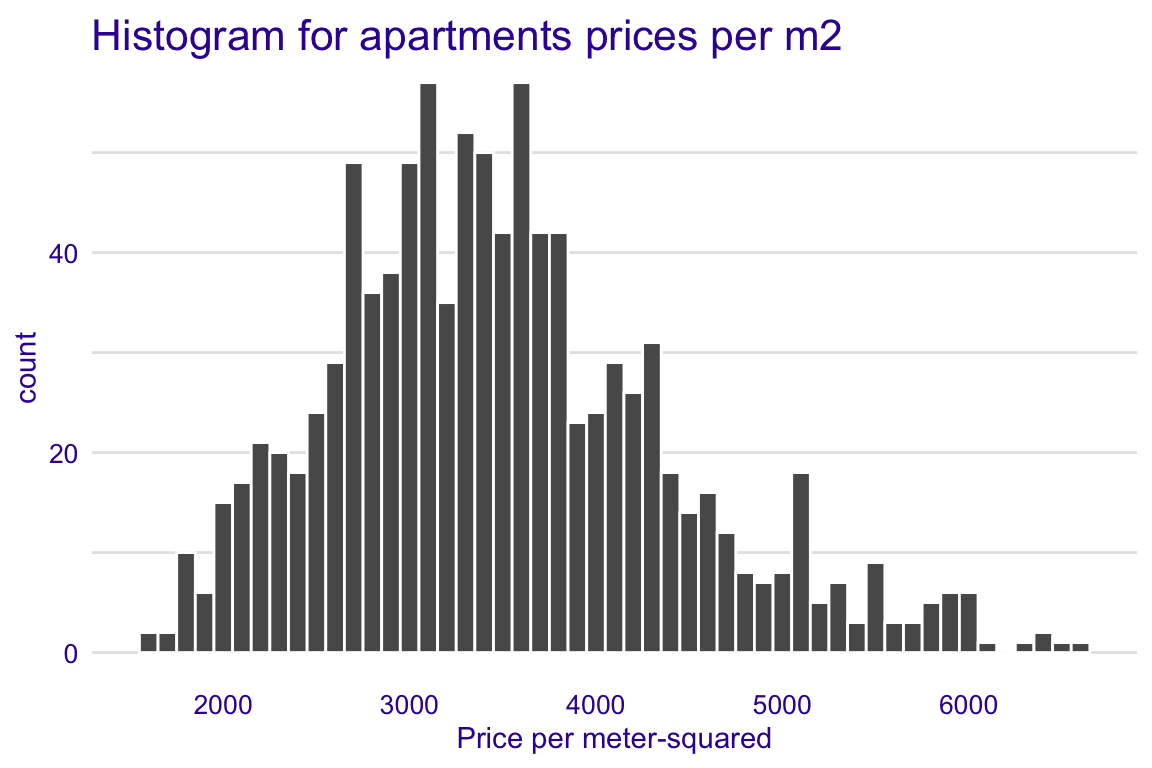
\includegraphics{PM_VEE_files/figure-latex/appartmentsExplorationMi2-1.pdf}

Figure \ref{fig:appartmentsMi2Construction} suggests (possibly) a nonlinear relation between \emph{construction.year} and \emph{m2.price}.

\begin{figure}
\centering
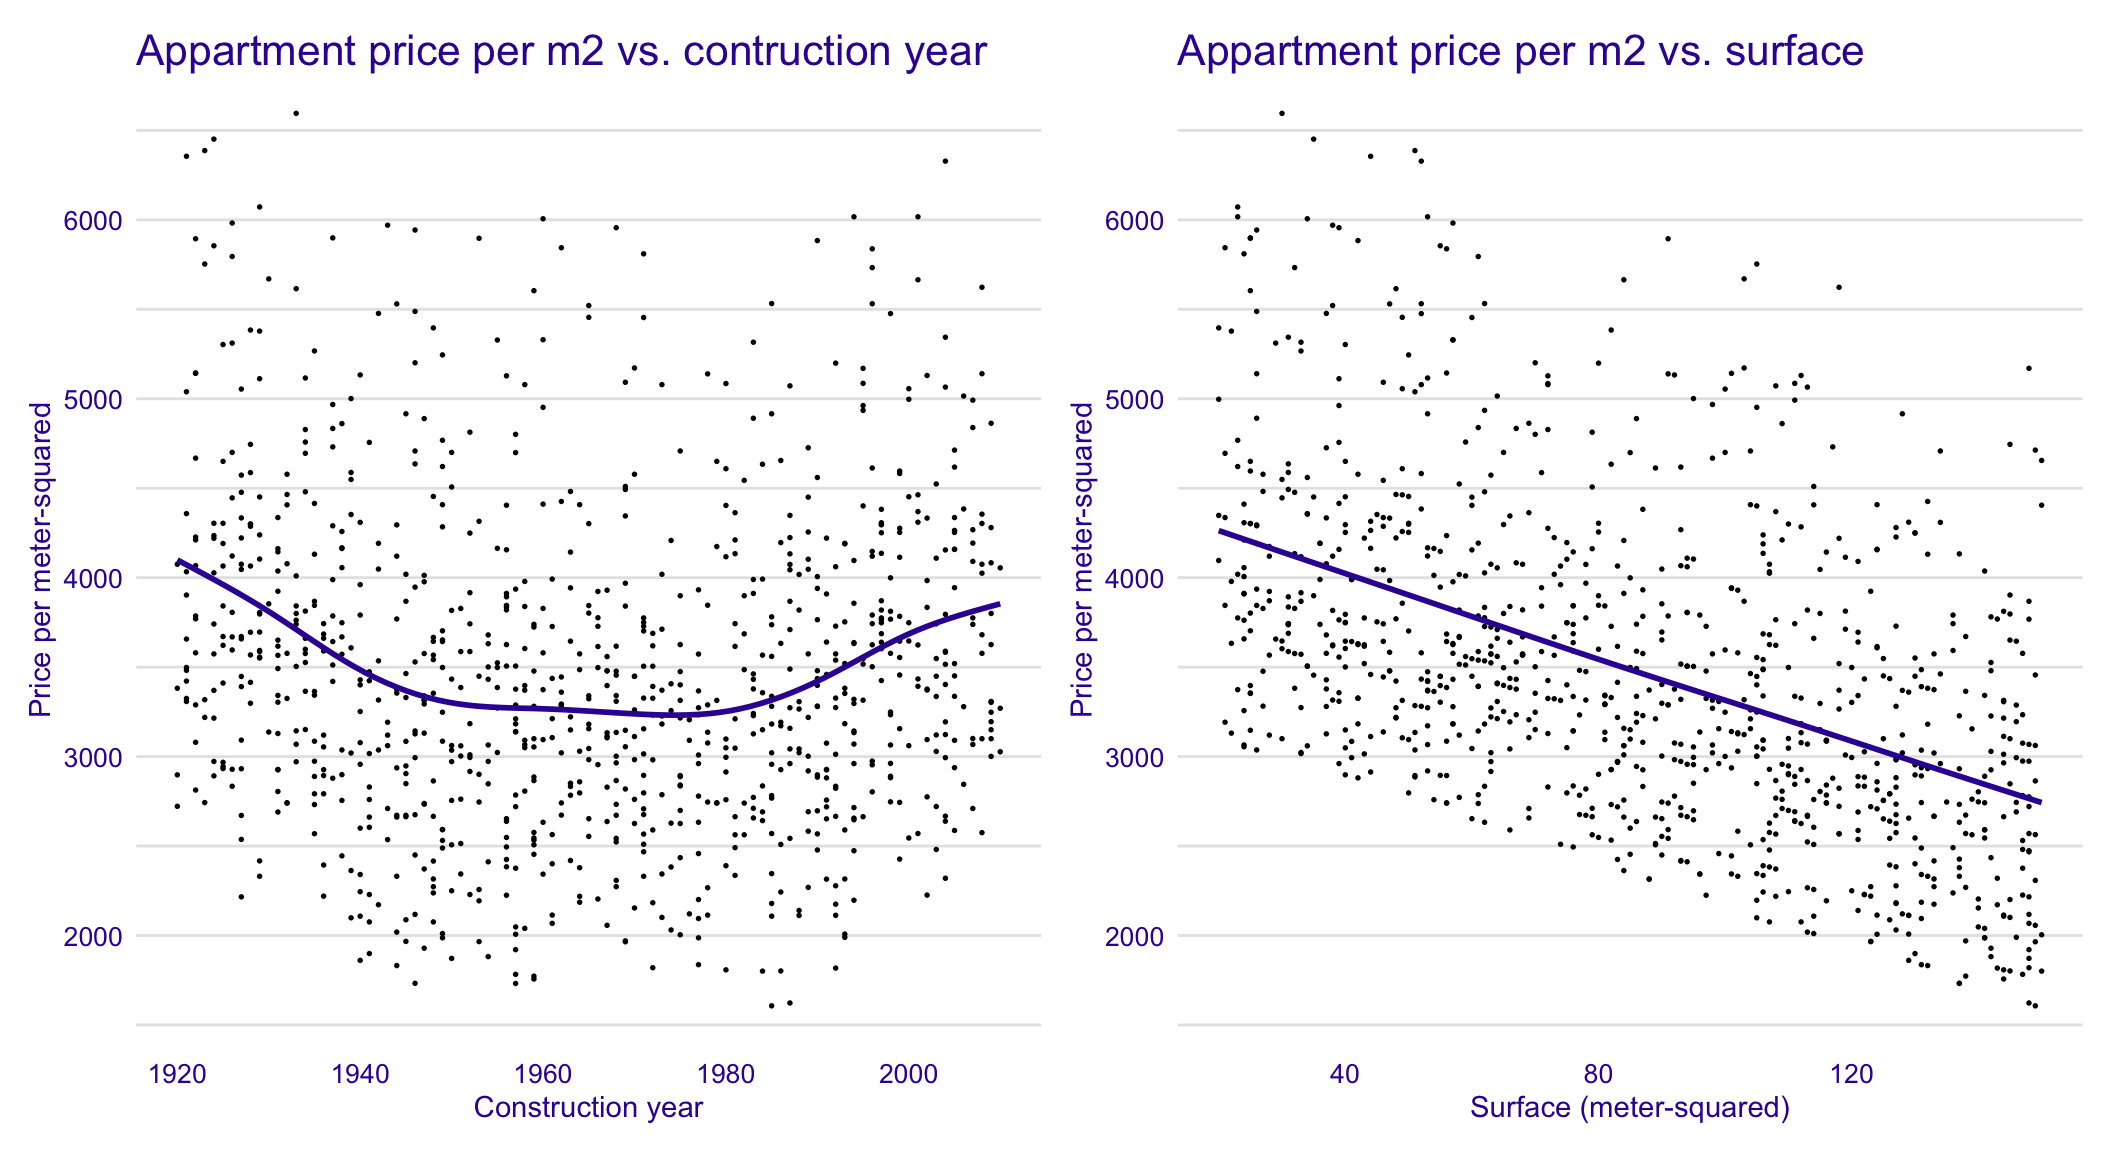
\includegraphics{PM_VEE_files/figure-latex/appartmentsMi2Construction-1.pdf}
\caption{\label{fig:appartmentsMi2Construction}(fig:appartmentsMi2Construction) Price per meter-squared vs.~construction year}
\end{figure}

Figure \ref{fig:appartmentsMi2Surface} indicates a linear relation between \emph{surface} and \emph{m2.price}.

\begin{figure}
\centering
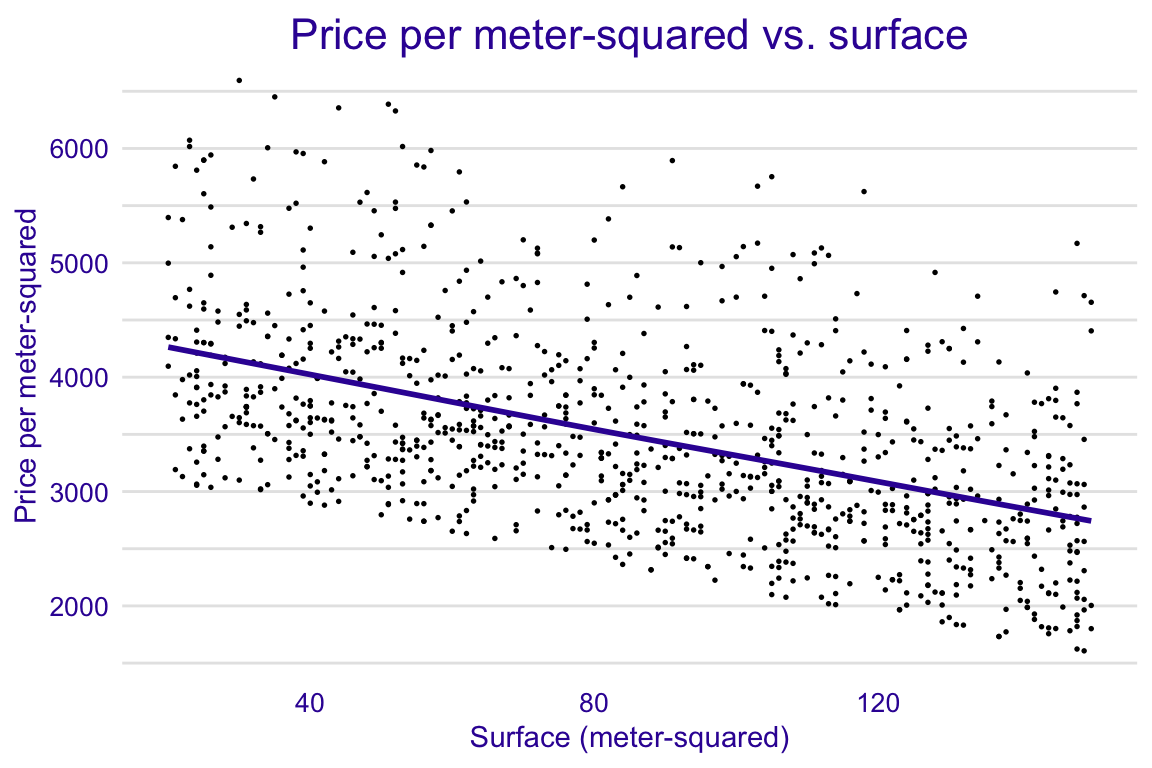
\includegraphics{PM_VEE_files/figure-latex/appartmentsMi2Surface-1.pdf}
\caption{\label{fig:appartmentsMi2Surface}(fig:appartmentsMi2Surface) Price per meter-squared vs.~surface}
\end{figure}

Relation between \emph{floor} and \emph{m2.price} is also close to linear, as seen in Figure \ref{fig:appartmentsMi2Floor}.

\begin{figure}
\centering
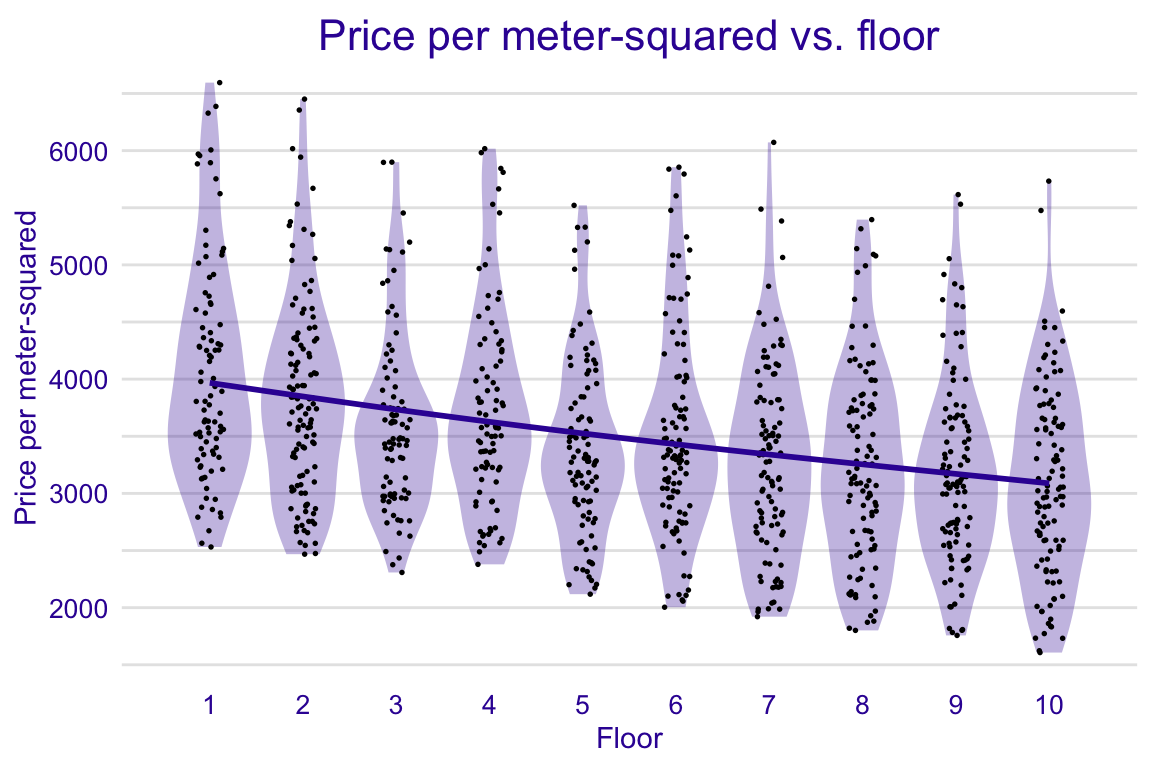
\includegraphics{PM_VEE_files/figure-latex/appartmentsMi2Floor-1.pdf}
\caption{\label{fig:appartmentsMi2Floor}(fig:appartmentsMi2Floor) Price per meter-squared vs.~floor}
\end{figure}

There is a close to linear relation between \emph{no.rooms} and \emph{m2.price}, as suggested by Figure \ref{fig:appartmentsMi2Norooms}. It is worth noting that, quite naturally, surface and number of rooms are correlated (see Figure \ref{fig:appartmentsSurfaceNorooms}).

\begin{figure}
\centering
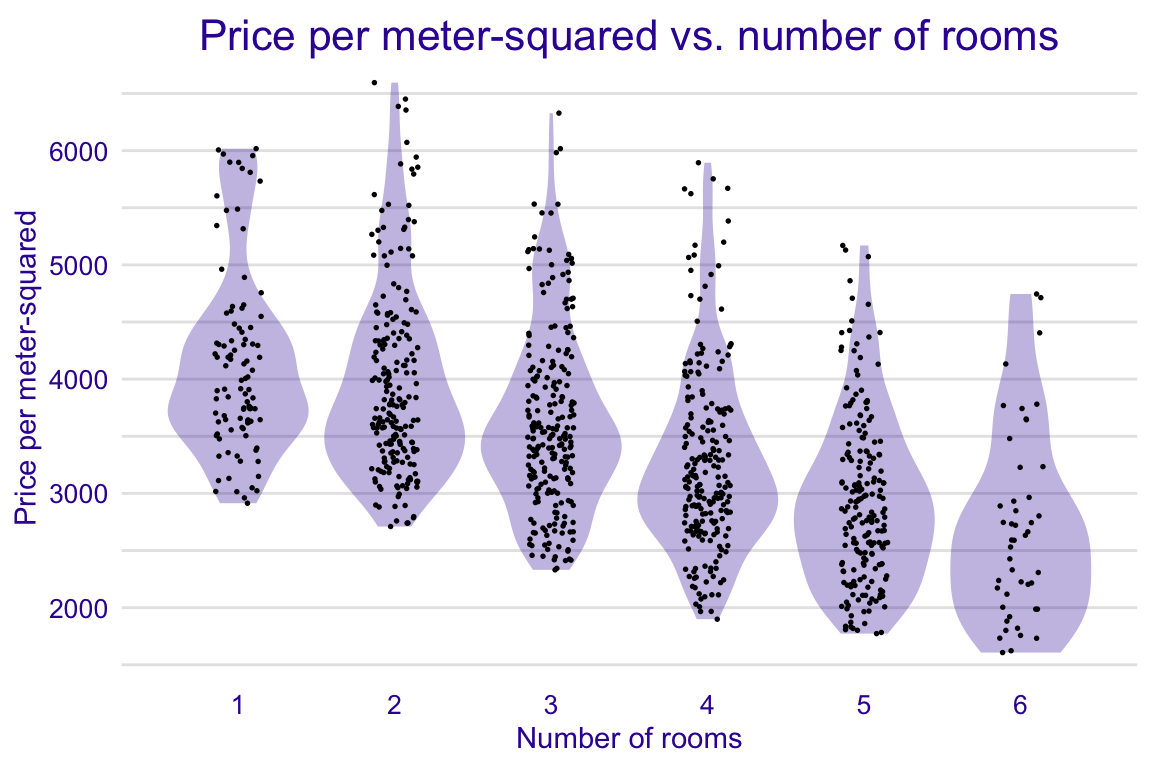
\includegraphics{PM_VEE_files/figure-latex/appartmentsMi2Norooms-1.pdf}
\caption{\label{fig:appartmentsMi2Norooms}(fig:appartmentsMi2Norooms) Price per meter-squared vs.~number of rooms}
\end{figure}

\begin{figure}
\centering
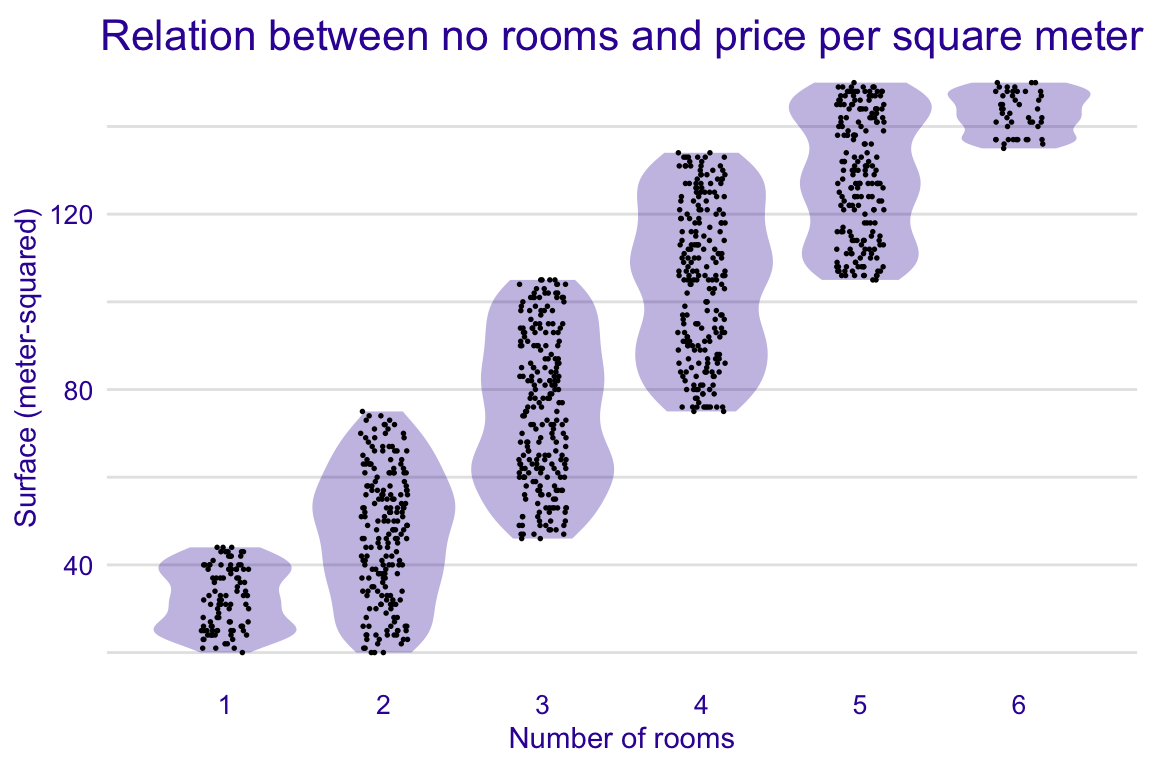
\includegraphics{PM_VEE_files/figure-latex/appartmentsSurfaceNorooms-1.pdf}
\caption{\label{fig:appartmentsSurfaceNorooms}(fig:appartmentsSurfaceNorooms) Surface vs.~number of rooms}
\end{figure}

Prices depend on district. Violin plots in Figure \ref{fig:appartmentsMi2District} indicate that the highest prices per meter-squared are observed in Srodmiescie (Downtown).

\begin{figure}
\centering
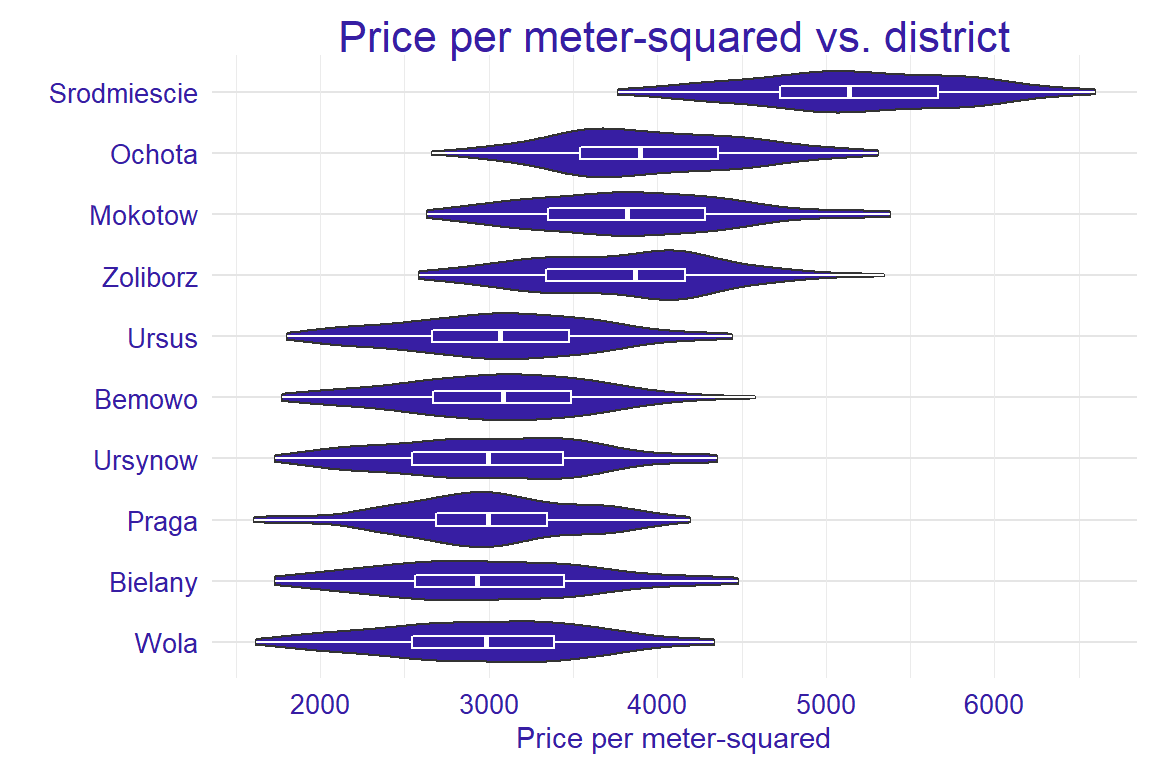
\includegraphics{PM_VEE_files/figure-latex/appartmentsMi2District-1.pdf}
\caption{\label{fig:appartmentsMi2District}(fig:appartmentsMi2District) Price per meter-squared for different districts}
\end{figure}

\hypertarget{model-Apartments-lr}{%
\subsubsection{Linear regression}\label{model-Apartments-lr}}

The dependent variable of interest, \emph{m2.price}, is continuous. Thus, a natural choice to build a predictive model is linear regression. We treat all the other variables in the \texttt{apartments} data frame as explanatory and include them in the model. The results of the model are stored in model-object \texttt{apartments\_lm\_v5}.

\begin{Shaded}
\begin{Highlighting}[]
\NormalTok{apartments_lm_v5 <-}\StringTok{ }\KeywordTok{lm}\NormalTok{(m2.price }\OperatorTok{~}\StringTok{ }\NormalTok{., }\DataTypeTok{data =}\NormalTok{ apartments)}
\NormalTok{apartments_lm_v5}
\end{Highlighting}
\end{Shaded}

\begin{verbatim}
## 
## Call:
## lm(formula = m2.price ~ ., data = apartments)
## 
## Coefficients:
##         (Intercept)    construction.year              surface  
##            5003.248               -0.229              -10.238  
##               floor             no.rooms      districtBielany  
##             -99.482              -37.730               34.106  
##       districtPraga      districtUrsynow       districtBemowo  
##             -20.214               -1.974               16.891  
##       districtUrsus     districtZoliborz      districtMokotow  
##              46.833              906.865              935.271  
##      districtOchota  districtSrodmiescie  
##             943.145             2097.502
\end{verbatim}

\hypertarget{model-Apartments-rf}{%
\subsubsection{Random forest}\label{model-Apartments-rf}}

As an alternative to linear regression, we consider a random forest model. To fit the model, we apply the \texttt{randomForest()} function, with default settings, from the package with the same name \citep{randomForestRNews}.\\
The results of the model are stored in model-object \texttt{apartments\_rf\_v5}.

\begin{Shaded}
\begin{Highlighting}[]
\KeywordTok{library}\NormalTok{(}\StringTok{"randomForest"}\NormalTok{)}
\KeywordTok{set.seed}\NormalTok{(}\DecValTok{72}\NormalTok{)}
\NormalTok{apartments_rf_v5 <-}\StringTok{ }\KeywordTok{randomForest}\NormalTok{(m2.price }\OperatorTok{~}\StringTok{ }\NormalTok{., }\DataTypeTok{data =}\NormalTok{ apartments)}
\NormalTok{apartments_rf_v5}
\end{Highlighting}
\end{Shaded}

\begin{verbatim}
## 
## Call:
##  randomForest(formula = m2.price ~ ., data = apartments) 
##                Type of random forest: regression
##                      Number of trees: 500
## No. of variables tried at each split: 1
## 
##           Mean of squared residuals: 79789.39
##                     % Var explained: 90.28
\end{verbatim}

\hypertarget{predictionsApartments}{%
\subsubsection{Model predictions}\label{predictionsApartments}}

By aplying the \texttt{predict()} function to model-object \texttt{apartments\_lm\_v5} with \texttt{apartments\_test} as the data frame for which predictions are to be computed, we obtain the predicted prices for the testing set of six apartments for the linear regression model. Subsequently, we compute the mean squared difference between the predicted and actual prices for the test apartments. We repeat the same steps for the random forest model.

\begin{Shaded}
\begin{Highlighting}[]
\NormalTok{predicted_apartments_lm <-}\StringTok{ }\KeywordTok{predict}\NormalTok{(apartments_lm_v5, apartments_test)}
\NormalTok{rmsd_lm <-}\StringTok{ }\KeywordTok{sqrt}\NormalTok{(}\KeywordTok{mean}\NormalTok{((predicted_apartments_lm }\OperatorTok{-}\StringTok{ }\NormalTok{apartments_test}\OperatorTok{$}\NormalTok{m2.price)}\OperatorTok{^}\DecValTok{2}\NormalTok{))}
\NormalTok{rmsd_lm}
\end{Highlighting}
\end{Shaded}

\begin{verbatim}
## [1] 283.0865
\end{verbatim}

\begin{Shaded}
\begin{Highlighting}[]
\NormalTok{predicted_apartments_rf <-}\StringTok{ }\KeywordTok{predict}\NormalTok{(apartments_rf_v5, apartments_test)}
\NormalTok{rmsd_rf <-}\StringTok{ }\KeywordTok{sqrt}\NormalTok{(}\KeywordTok{mean}\NormalTok{((predicted_apartments_rf }\OperatorTok{-}\StringTok{ }\NormalTok{apartments_test}\OperatorTok{$}\NormalTok{m2.price)}\OperatorTok{^}\DecValTok{2}\NormalTok{))}
\NormalTok{rmsd_rf}
\end{Highlighting}
\end{Shaded}

\begin{verbatim}
## [1] 282.9519
\end{verbatim}

For the random forest model, the square-root of the mean squared difference is equal to 283. It is only minimally smaller than the value of 283.1, obtained for the linear regression model. Thus, the question we may face is: should we choose the more complex, but flexible random-forest model, or the simpler and easier to interpret linear model? In the subsequent chapters we will try to provide an answer to this question.

\hypertarget{ExplainersApartmentsRCode}{%
\subsubsection{Explainers}\label{ExplainersApartmentsRCode}}

In similar spirit to the Section \ref{ExplainersTitanicRCode} we will use explainers also for predictive models created for the \texttt{apartments} dataset.

\begin{Shaded}
\begin{Highlighting}[]
\NormalTok{explain_apartments_lm_v5 <-}\StringTok{ }\KeywordTok{explain}\NormalTok{(}\DataTypeTok{model =}\NormalTok{ apartments_lm_v5, }
                                 \DataTypeTok{data =}\NormalTok{ apartments_test,}
                                 \DataTypeTok{y =}\NormalTok{ apartments_test}\OperatorTok{$}\NormalTok{m2.price,}
                                 \DataTypeTok{label =} \StringTok{"Linear Regression v5"}\NormalTok{)}
\NormalTok{explain_apartments_rf_v5 <-}\StringTok{ }\KeywordTok{explain}\NormalTok{(}\DataTypeTok{model =}\NormalTok{ apartments_rf_v5, }
                                 \DataTypeTok{data =}\NormalTok{ apartments_test,}
                                 \DataTypeTok{y =}\NormalTok{ apartments_test}\OperatorTok{$}\NormalTok{m2.price,}
                                 \DataTypeTok{label =} \StringTok{"Random Forest v5"}\NormalTok{)}
\end{Highlighting}
\end{Shaded}

\hypertarget{ListOfModelsApartments}{%
\subsubsection{\texorpdfstring{List of objects for the \texttt{apartments} example}{List of objects for the apartments example}}\label{ListOfModelsApartments}}

In Sections \ref{model-Apartments-lr} and \ref{model-Apartments-rf} we have built two predictive models for the \texttt{apartments} data set. The models will be used in the rest of the book to illustrate the model explanation methods and tools.

For the ease of reference, we summarize the models in Table \ref{tab:archivistHooksOfModelsApartments}. The binary model-objects can be downloaded by using the indicated \texttt{archivist} hooks \citep{archivist}. By calling a function specified in the last column of the table, one can recreate a selected model in a local R environment.

\begin{longtable}[]{@{}llll@{}}
\caption{\label{tab:archivistHooksOfModelsApartments} Predictive models created for the \texttt{apartments} dataset.}\tabularnewline
\toprule
\begin{minipage}[b]{0.21\columnwidth}\raggedright
Model name\strut
\end{minipage} & \begin{minipage}[b]{0.25\columnwidth}\raggedright
Model generator\strut
\end{minipage} & \begin{minipage}[b]{0.18\columnwidth}\raggedright
Variables\strut
\end{minipage} & \begin{minipage}[b]{0.25\columnwidth}\raggedright
Archivist hooks\strut
\end{minipage}\tabularnewline
\midrule
\endfirsthead
\toprule
\begin{minipage}[b]{0.21\columnwidth}\raggedright
Model name\strut
\end{minipage} & \begin{minipage}[b]{0.25\columnwidth}\raggedright
Model generator\strut
\end{minipage} & \begin{minipage}[b]{0.18\columnwidth}\raggedright
Variables\strut
\end{minipage} & \begin{minipage}[b]{0.25\columnwidth}\raggedright
Archivist hooks\strut
\end{minipage}\tabularnewline
\midrule
\endhead
\begin{minipage}[t]{0.21\columnwidth}\raggedright
\texttt{apartments\_lm\_v5}\strut
\end{minipage} & \begin{minipage}[t]{0.25\columnwidth}\raggedright
\texttt{stats::\ lm} v.3.5.3\strut
\end{minipage} & \begin{minipage}[t]{0.18\columnwidth}\raggedright
construction .year, surface, floor, no.rooms, district\strut
\end{minipage} & \begin{minipage}[t]{0.25\columnwidth}\raggedright
Get the model: \texttt{archivist::\ aread("pbiecek/models/55f19")}. Get the explainer: \texttt{archivist::\ aread("pbiecek/models/f49ea")}\strut
\end{minipage}\tabularnewline
\begin{minipage}[t]{0.21\columnwidth}\raggedright
\texttt{apartments\_rf\_v5}\strut
\end{minipage} & \begin{minipage}[t]{0.25\columnwidth}\raggedright
\texttt{randomForest::\ randomForest} v.4.6.14\strut
\end{minipage} & \begin{minipage}[t]{0.18\columnwidth}\raggedright
construction .year, surface, floor, no.rooms, district\strut
\end{minipage} & \begin{minipage}[t]{0.25\columnwidth}\raggedright
Get the model: \texttt{archivist::\ aread("pbiecek/models/fe7a5")}. Get the explainer: \texttt{archivist::\ aread("pbiecek/models/569b0")}\strut
\end{minipage}\tabularnewline
\bottomrule
\end{longtable}

\hypertarget{InstanceLevelExploration}{%
\section{Instance-level exploration}\label{InstanceLevelExploration}}

\begin{figure}

{\centering 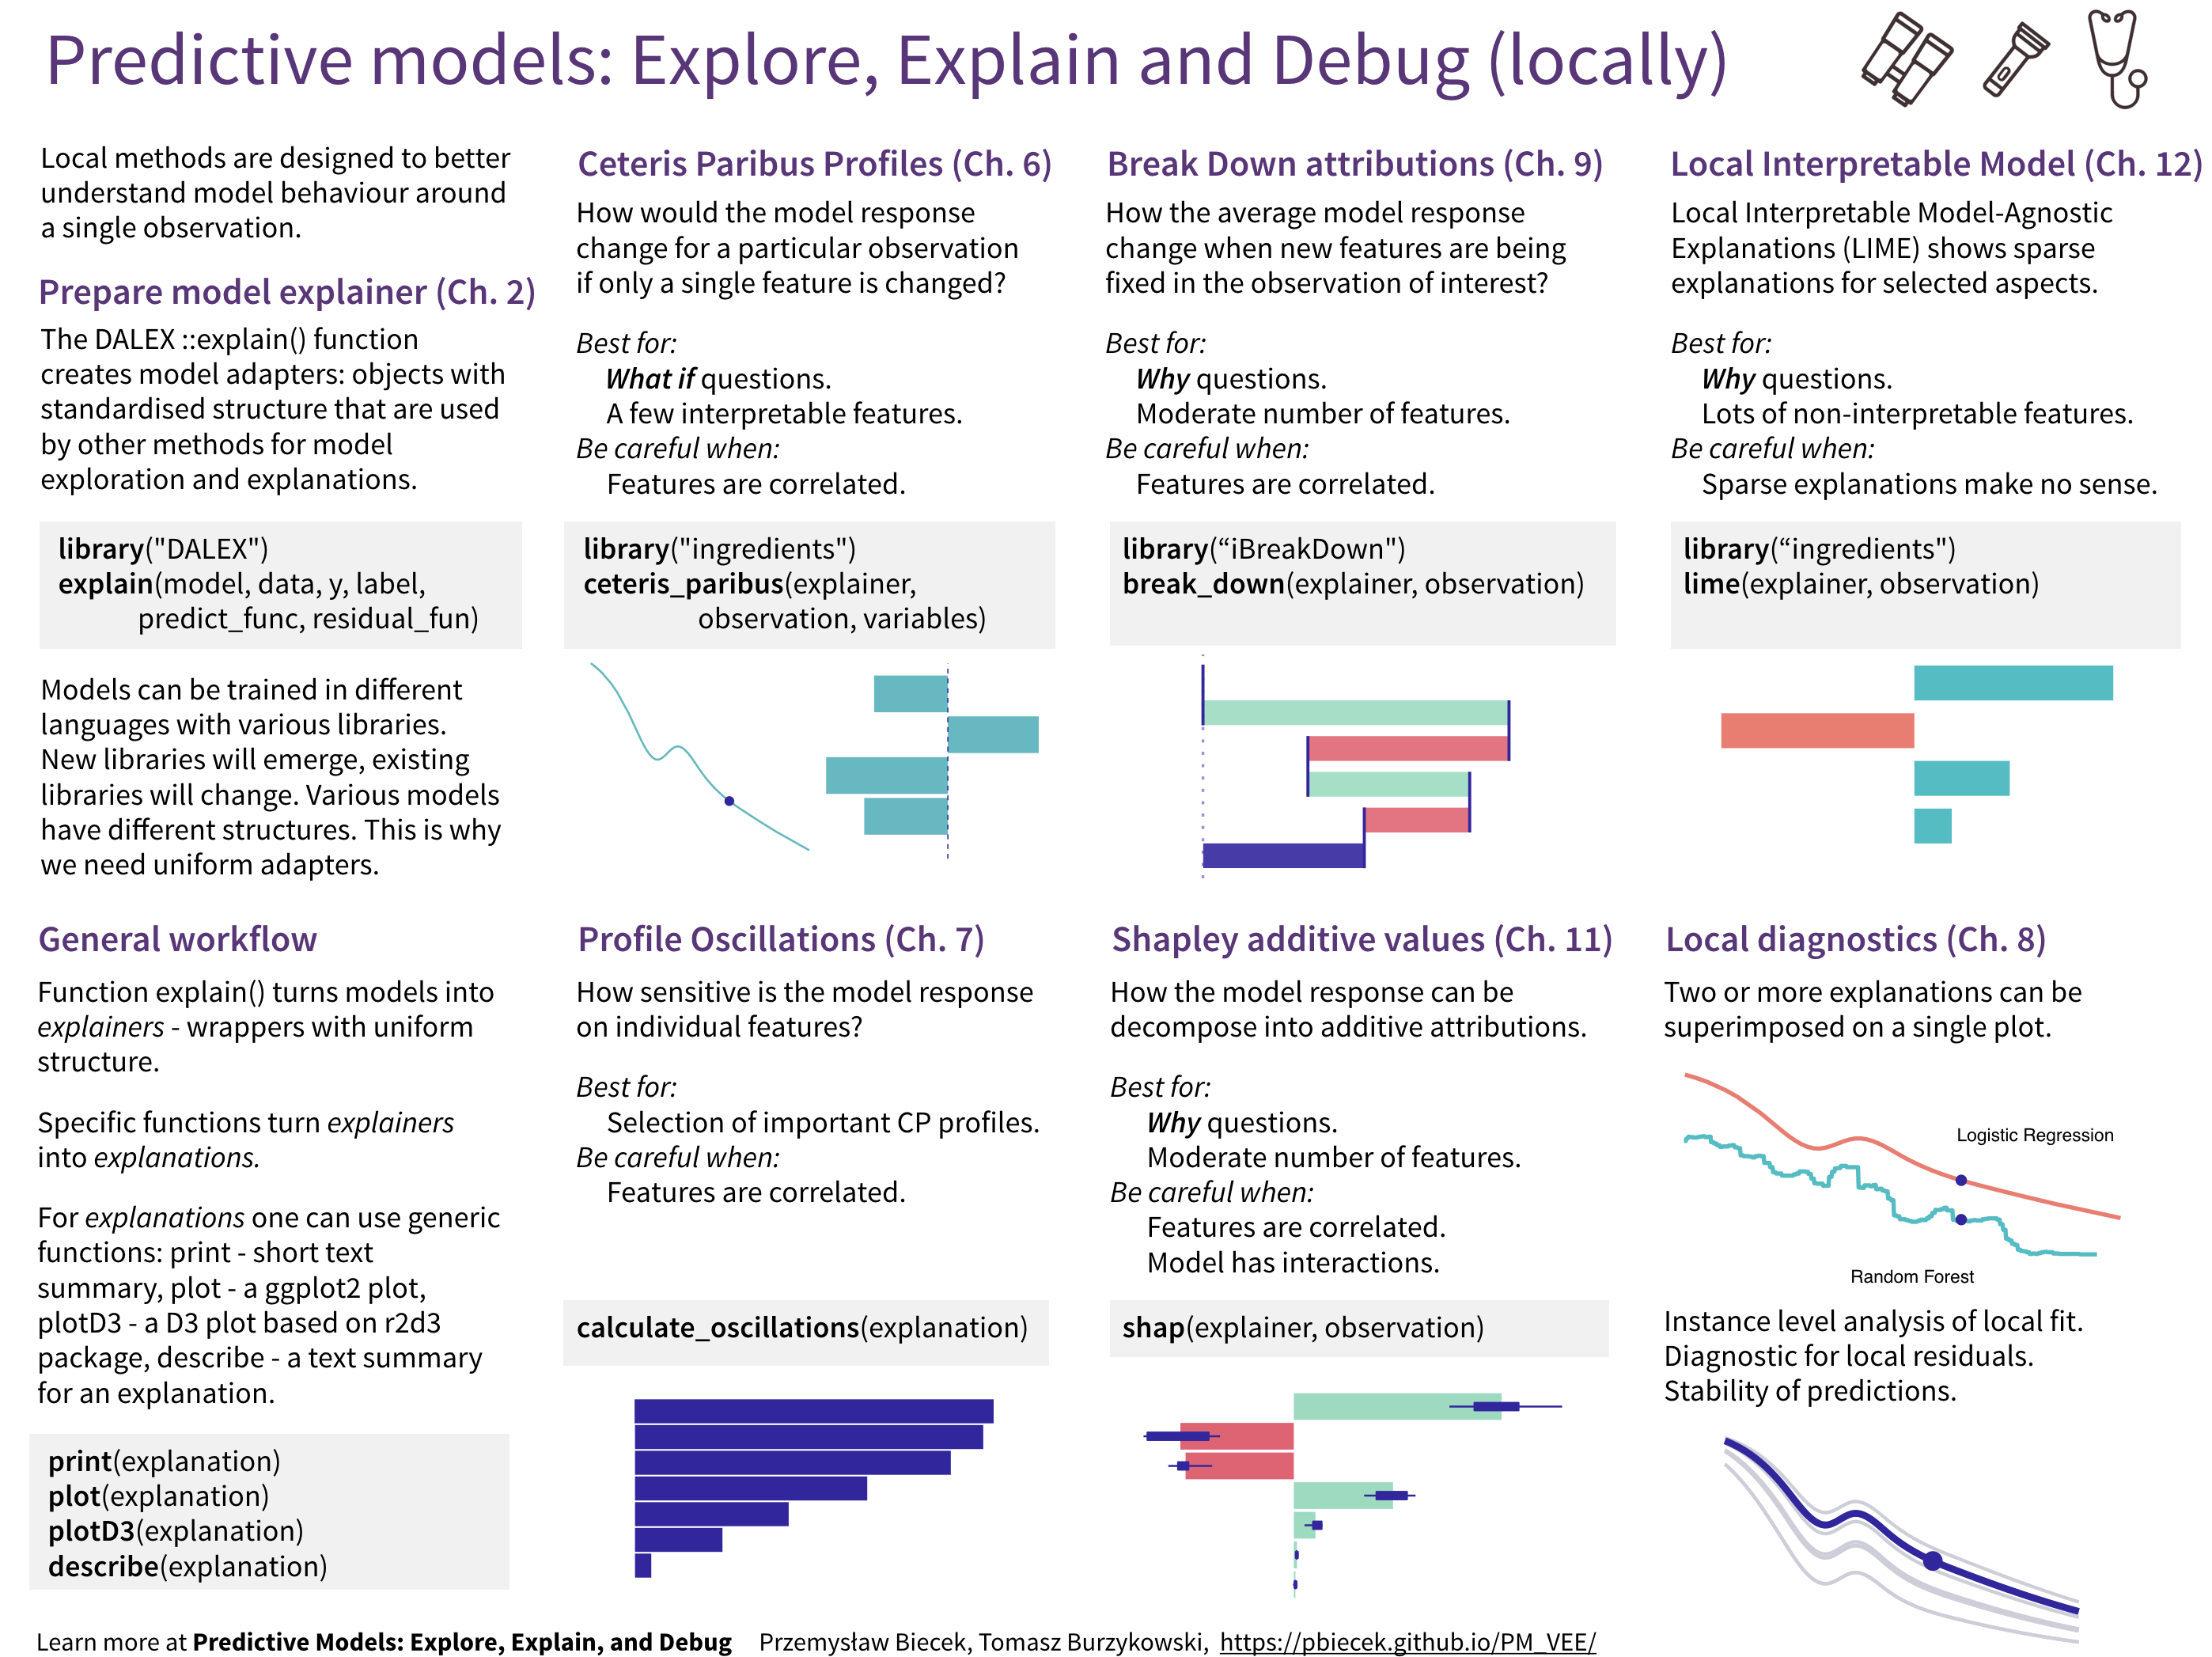
\includegraphics[width=0.99\linewidth]{figure/cheatsheet_local_explainers} 

}

\caption{(fig:localDALEXsummary) Summary of differnet approaches to local model exploration and explanation.}\label{fig:localDALEXsummary}
\end{figure}

Instance-level explainers help to understand how a model yields a prediction for a single observation. We can think about the following situations as examples:

\begin{itemize}
\tightlist
\item
  We may want to evaluate the effects of explanatory variables on model predictions. For instance, we may be interested in predicting the risk of heart attack based on person's age, sex, and smoking habits. A model may be used to construct a score (for instance, a linear combination of the explanatory variables representing age, sex, and smoking habits) that could be used for the purposes of prediction. For a particular patient we may want to learn how much the different variables contribute to the patient's score?
\item
  We may want to understand how models predictions would change if values of some of the explanatory variables changed. For instance, what would be the predicted risk of heart attack if the patient cut the number of cigarettes smoked per day by half?
\item
  We may discover that the model is providing incorrect predictions and we may want to find the reason. For instance, a patient with a very low risk-score experiences heart attack. What has driven that prediction?
\end{itemize}

A model is a function with a \(p\)-dimensional vector \(x\) as an argument. The plot of the value(s) of the function can be constructed in a \(p+1\)-dimensional space. An example with \(p=2\) is presented in Figure \ref{fig:cutsSurfaceReady}. We will use it as an illustration of key ideas. The plot provides an information about the values of the function in the vicinity of point \(x^*\).

\begin{figure}

{\centering 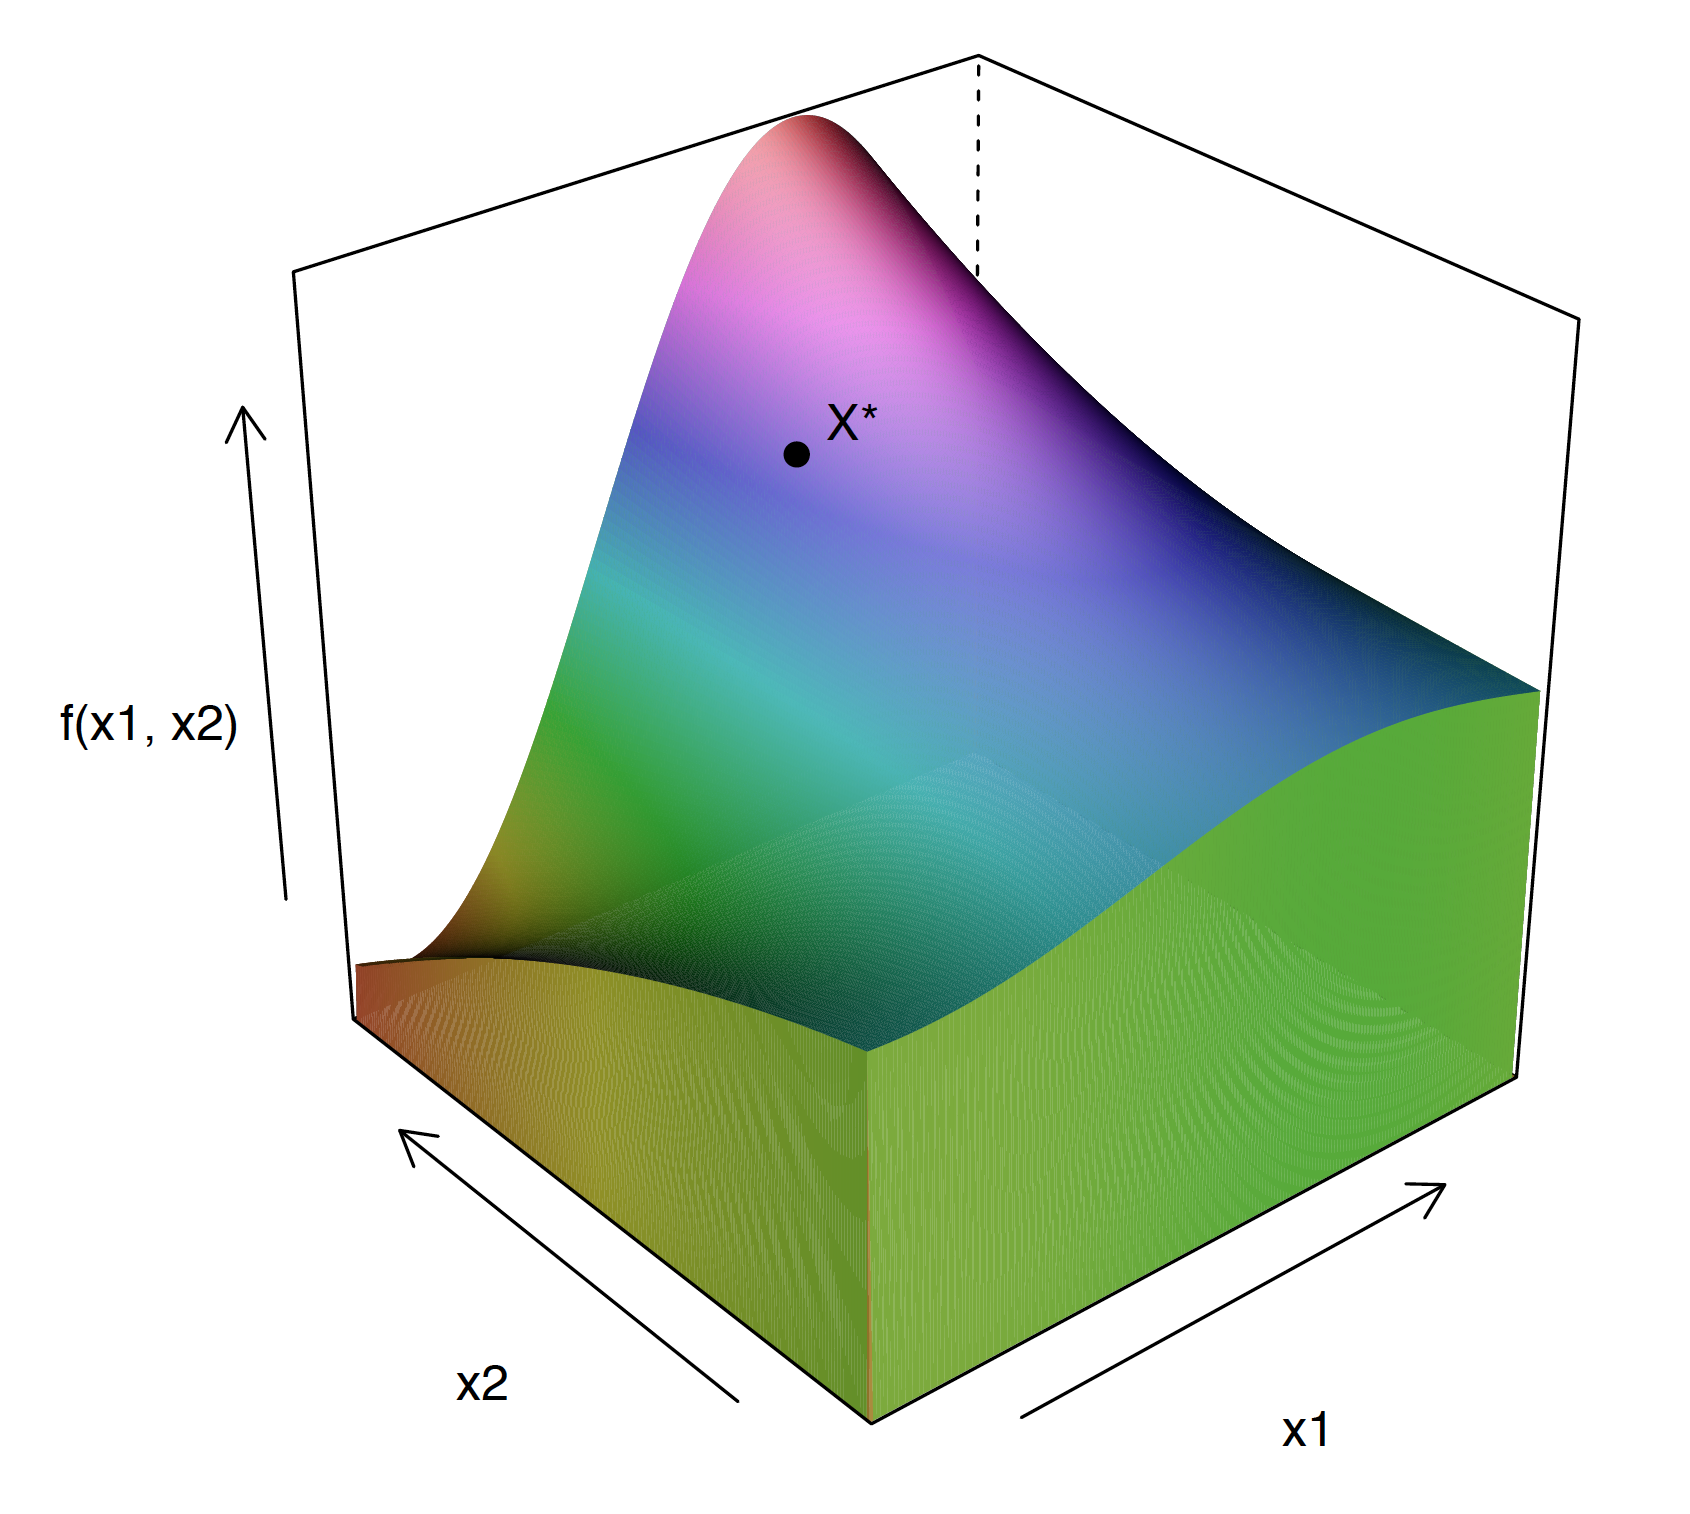
\includegraphics[width=0.6\linewidth]{figure/cuts_surface_ready_punkt} 

}

\caption{(fig:cutsSurfaceReady) Response surface for a model that is a function of two variables. We are interested in understanding the response of a model in a single point x*}\label{fig:cutsSurfaceReady}
\end{figure}

There are many different tools that may be used to explore the predictions of the model around a single point \(x^*\). In the following sections we will describe the most popular approaches. They can be divided into three classes.

\begin{itemize}
\tightlist
\item
  One approach is to investigate how the model prediction changes if the value of a single explanatory variable changes. The approach is useful in the so-called ,,What-If'' analyses. In particular, we can construct plots presenting the change in model-based predictions induced by a change of a single variable. Such plots are usually called Ceteris-paribus (CP) profiles. An example is provided in panel A of Figure \ref{fig:cutsTechnikiReady}. Chapters \ref{ceterisParibus}-\ref{localDiagnostics} introduce the CP profiles and methods based on them.\\
\item
  Another approach is to analyze how the model prediction for point \(x^*\) is different from the average model prediction and how the difference can be distributed among explanatory variables. It is often called the ,,variable attributions'' approach. An example is provided in panel B of Figure \ref{fig:cutsTechnikiReady}. Chapters \ref{breakDown}-\ref{shapley} present various methods implementing this approach.
\item
  Yet another approach is to analyze the curvature of the response surface (see Figure \ref{fig:cutsSurfaceReady}) around the point of interest \(x^*\). Treating the model as a function, we are interested in the local behavior of this function around \(x^*\). In case of a black-box model, we may approximate it with a simpler glass-box model around \(x^*\). An example is provided in panel C of Figure \ref{fig:cutsTechnikiReady}. Chapter \ref{LIME} presents the Local Interpretable Model-agnostic Explanations (LIME) method that exploits the concept of a ,,local model.''
\end{itemize}

Each method has its own merits and limitations. They are briefly discussed in the corresponding chapters. Chapter \ref{SummaryInstanceLevel} offers a comparison of the methods.

\begin{figure}

{\centering 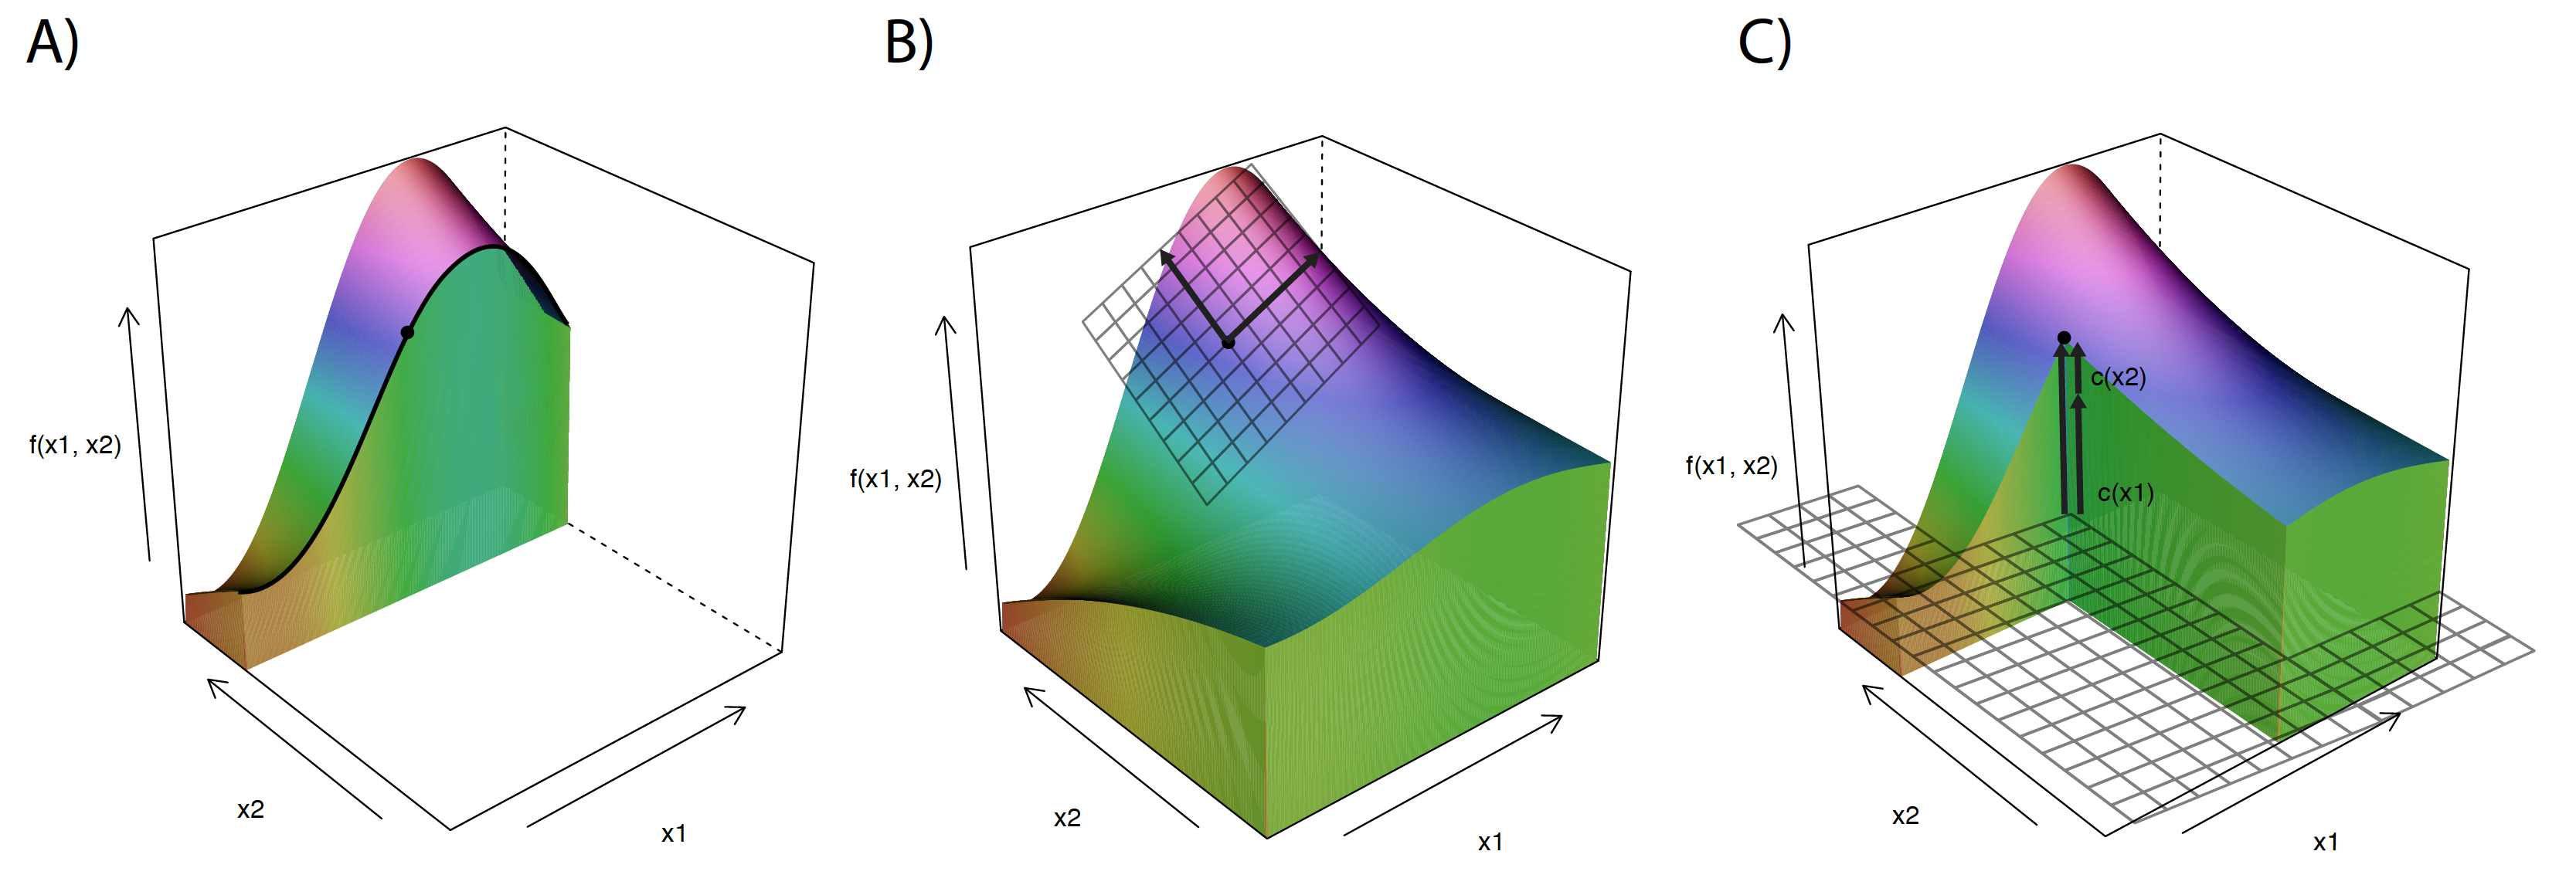
\includegraphics[width=0.99\linewidth]{figure/cuts_techniki_ready} 

}

\caption{(fig:cutsTechnikiReady) Illustration of different approaches to instance-level explanation. Panel A presents a What-If analysis with Ceteris-paribus profiles. The profiles show the model response as a function of a value of a single variable, while keeping the values of all other explanatory variables fixed. Panel B illustrates the concept of variable attributions. Additive effects of each variable show how the model response differs from the average. Panel C illustrates the concept of local models. A simpler glass-box model is fitted around the point of interest. It describes the local behaviour of the black-box model. }\label{fig:cutsTechnikiReady}
\end{figure}

\hypertarget{ceterisParibus}{%
\section{Ceteris-paribus Profiles and What-If Analysis}\label{ceterisParibus}}

\hypertarget{CPIntro}{%
\subsection{Introduction}\label{CPIntro}}

\emph{Ceteris paribus} is a Latin phrase meaning ``other things held constant'' or ``all else unchanged.'' In this chapter, we introduce a technique for model exploration based on the \emph{Ceteris paribus} principle. In particular, we examine the influence of each explanatory variable, assuming that effects of all other variables are unchanged. The main goal is to understand how changes in a single explanatory variable affects model predictions.

Explanation tools (explainers) presented in this chapter are linked to the second law introduced in Section \ref{three-single-laws}, i.e.~the law of ``Prediction's speculation.'' This is why the tools are also known as \emph{What-If model analysis} or \emph{Individual Conditional Expectations} \citep{ICEbox}. It appears that it is easier to understand how a black-box model is working if we can explore the model by investigating the influence of explanatory variables separately, changing one at a time.

\hypertarget{CPIntuition}{%
\subsection{Intuition}\label{CPIntuition}}

Panel A of Figure \ref{fig:modelResponseCurveLine} presents response (prediction) surface for the \texttt{titanic\_lmr\_v6} model for two explanatory variables, \emph{age} and \emph{class}, from the \emph{titanic} dataset (see Section \ref{TitanicDataset}). We are interested in the change of the model prediction induced by each of the variables. Toward this end, we may want to explore the curvature of the response surface around a single point with \emph{age} equal to 47 and \emph{class} equal to ``1st,'' indicated in the plot. Ceteris-paribus (CP) profiles are one-dimensional profiles that examine the curvature across each dimension, i.e., for each variable. Panel B of Figure \ref{fig:modelResponseCurveLine} presents the profiles corresponding to \emph{age} and \emph{class}. Note that, in the CP profile for \emph{age}, the point of interest is indicated by the black dot. In essence, a CP profile shows a conditional expectation of the dependent variable (response) for the particular explanatory variable.

\begin{figure}

{\centering 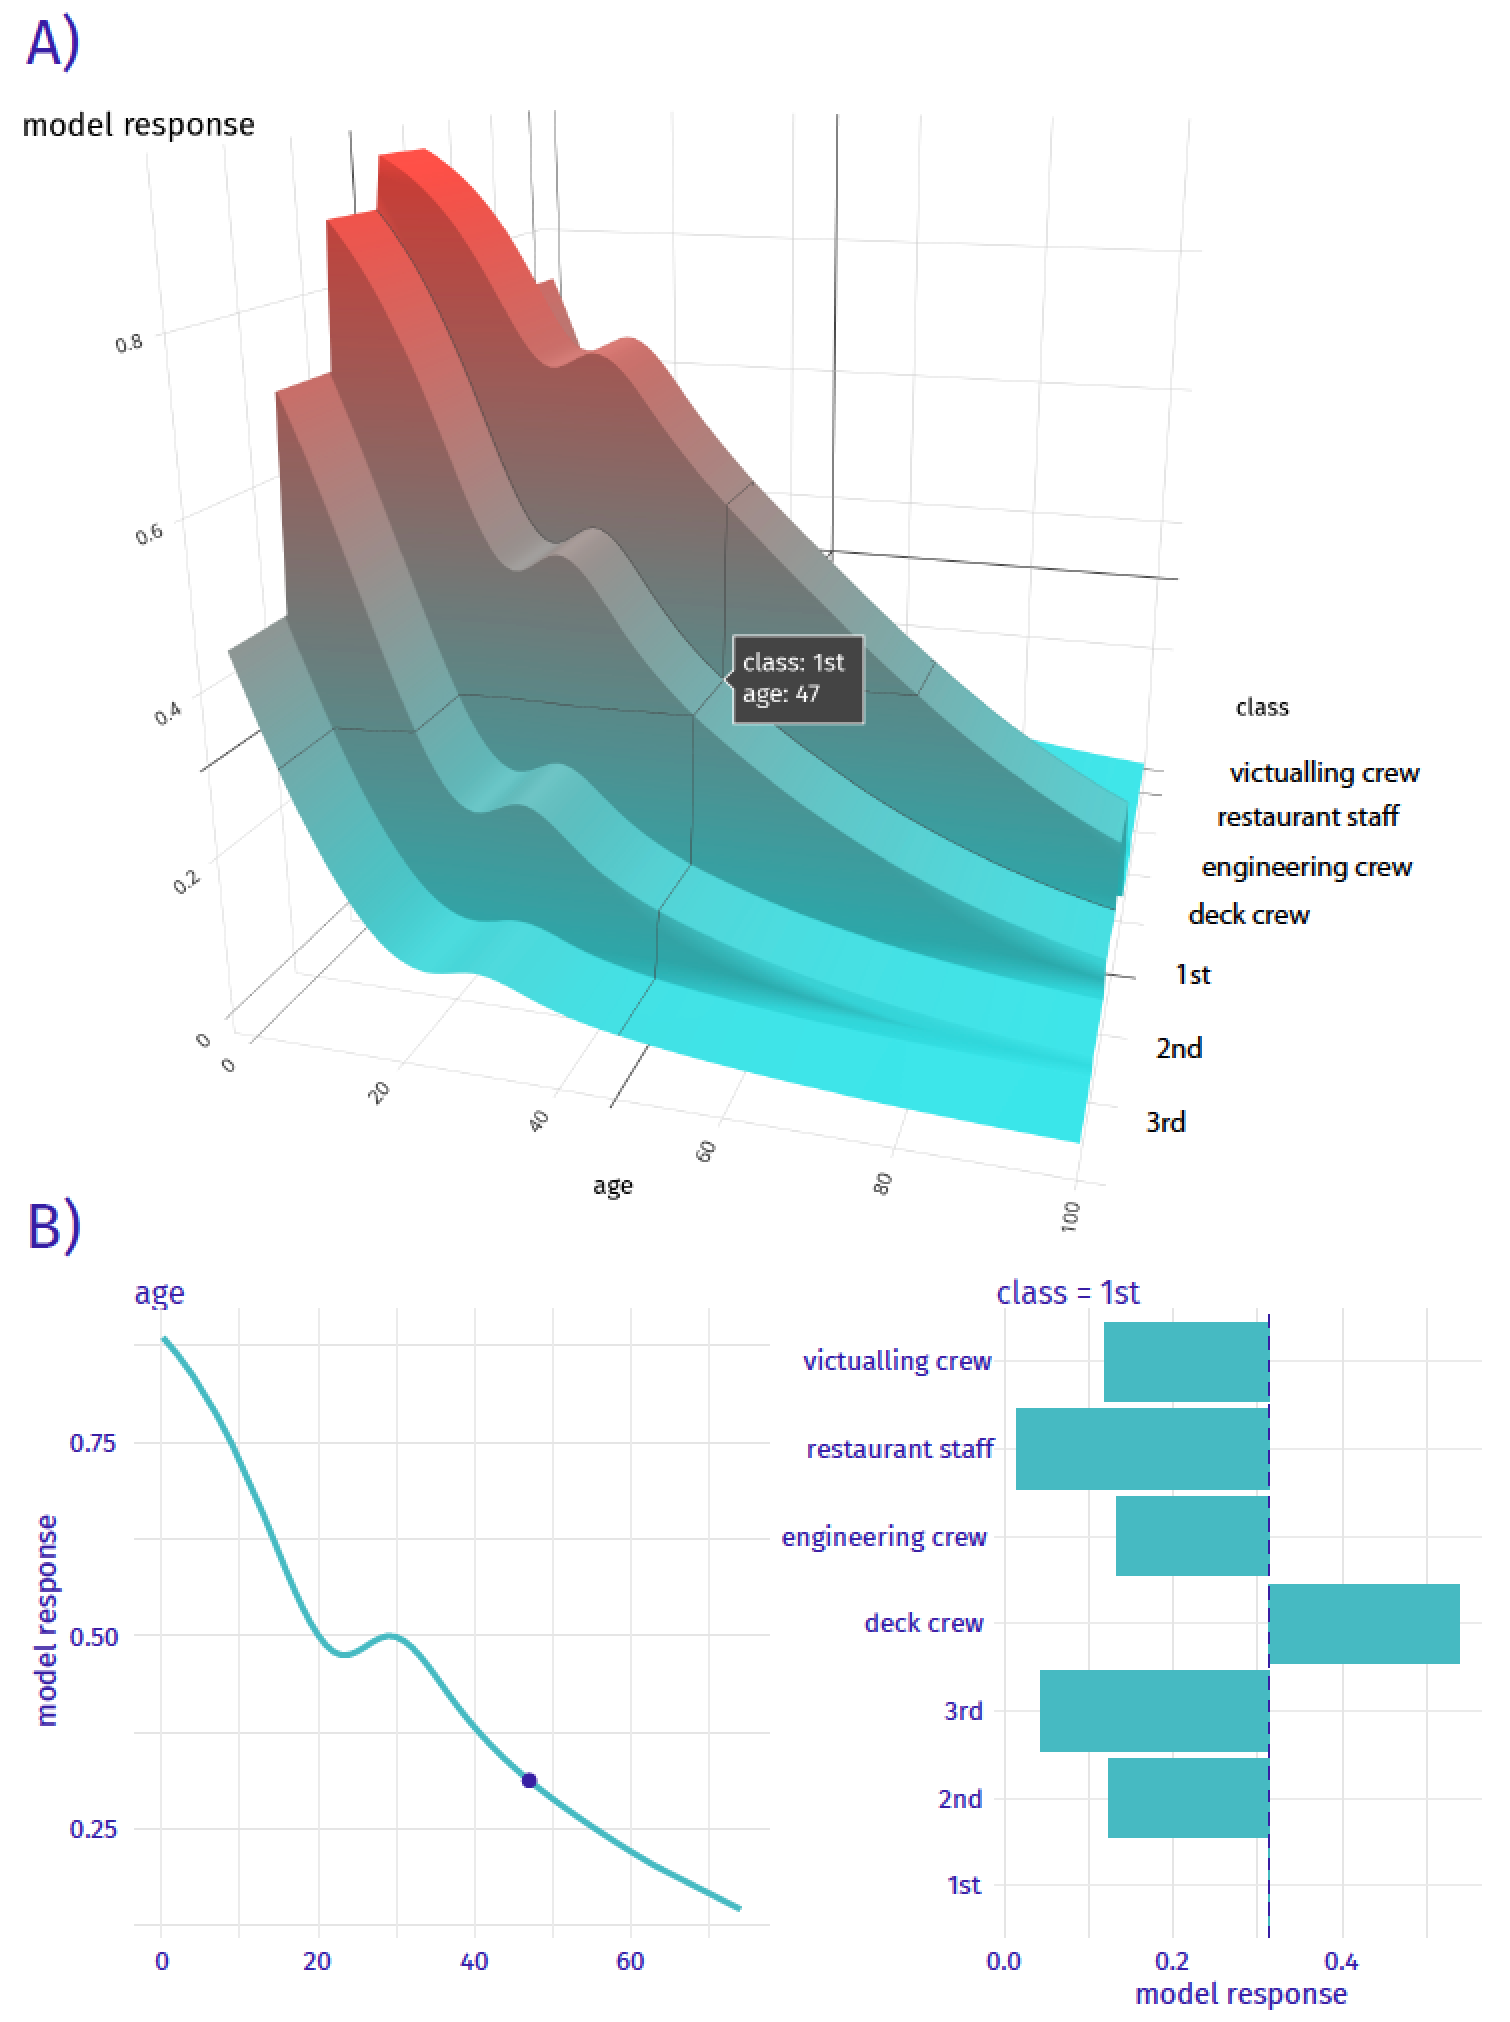
\includegraphics[width=0.7\linewidth]{figure/profile_age_class} 

}

\caption{(fig:modelResponseCurveLine) A) Model response (prediction) surface. Ceteris-paribus (CP) profiles marked with black curves help to understand the curvature of the surface while changing only a single explanatory variable. B) CP profiles for individual variables, age (continuous) and class (categorical).}\label{fig:modelResponseCurveLine}
\end{figure}

\begin{figure}

{\centering 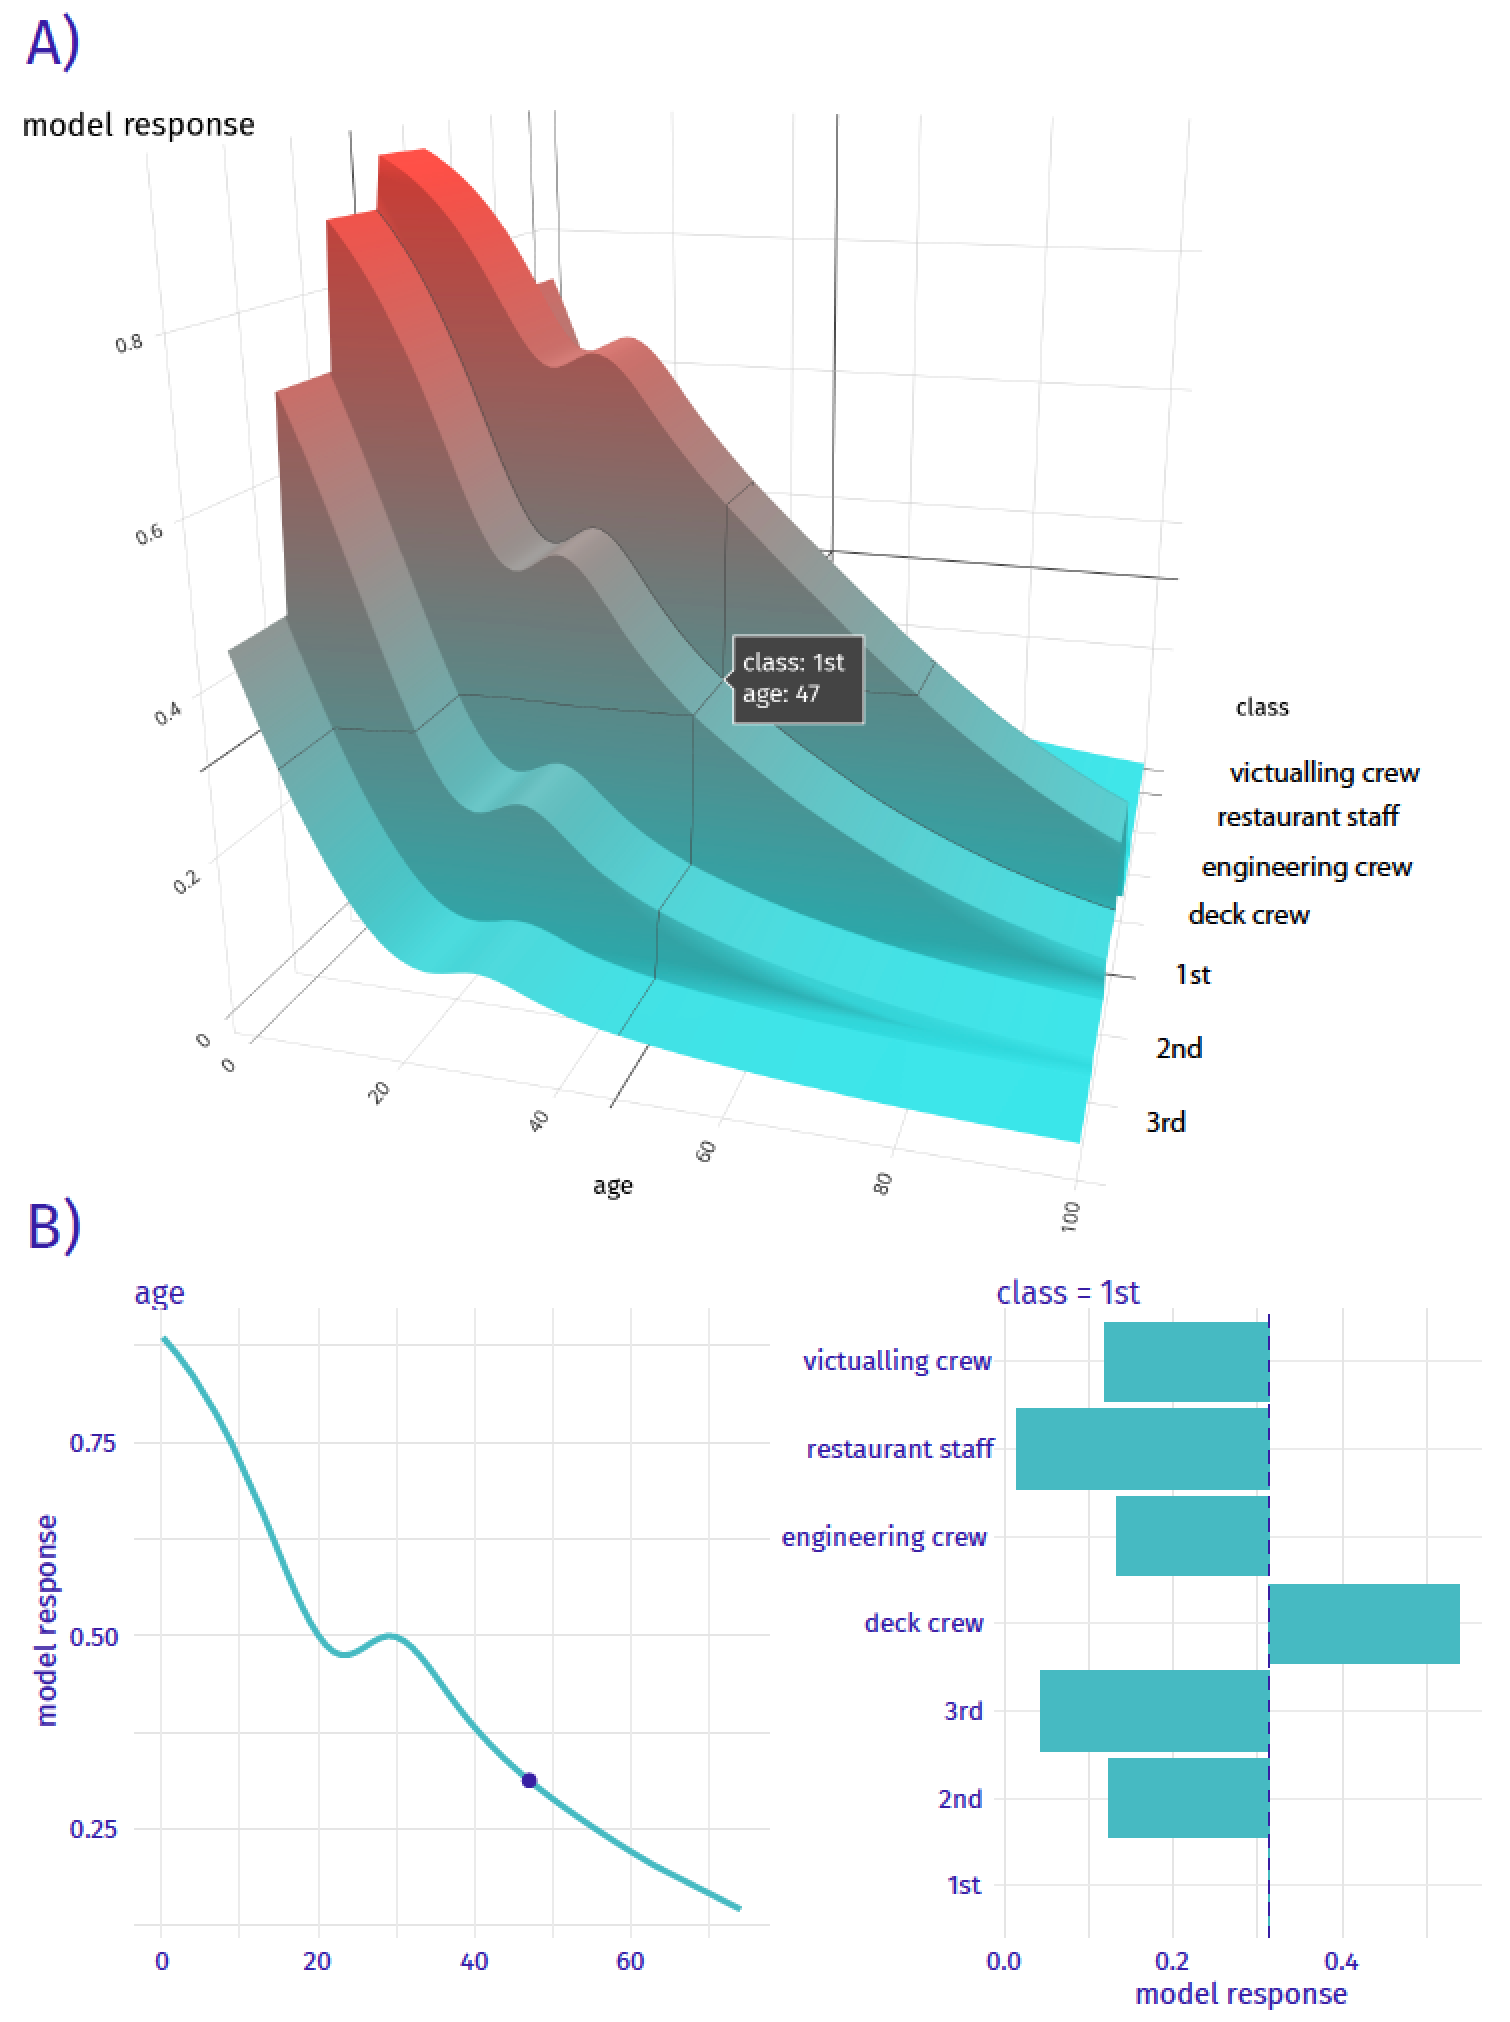
\includegraphics[width=0.7\linewidth]{figure/profile_age_class} 

}

\caption{(fig:modelResponseCurveAnimation) Animated model response 2D surface as in (fig:modelResponseCurveLine).}\label{fig:modelResponseCurveAnimation}
\end{figure}

CP belongs to the class of techniques that examine local curvature of the model response surface. Other very popular technique from this class called LIME is presented in Chapter \ref{LIME}.

CP technique is similar to the LIME method (see Chapter \ref{LIME}). LIME and CP profiles examine the curvature of response surface of a model. The difference between these two methods lies in the fact that LIME approximates the model of interest locally with a simpler glass-box model. Usually, the LIME model is sparse, i.e., contains fewer explanatory variables. Thus, one needs to investigate a plot across a smaller number of dimensions. On the other hand, the CP profiles present conditional predictions for every variable and, in most cases, are easier to interpret. More detailed comparison of these techniques is presented in the Chapter \ref{summaryInstanceLevel}.

\hypertarget{CPMethod}{%
\subsection{Method}\label{CPMethod}}

In this section, we introduce more formally one-dimensional CP profiles.

In predictive modeling, we are interested in a distribution of a dependent variable \(Y\) given vector \(x_*\). The latter contains values of explanatory variables. In the ideal world, we would like to know the conditional distribution of \(Y\) given \(x_*\). In practical applications, however, we usually do not predict the entire distribution, but just some of its characteristics like the expected (mean) value, a quantile, or variance. Without loss of generality we will assume that we model the conditional expected value \(E_Y(Y | x_*)\).

Assume that we have got model \(f()\), for which \(f(x_*)\) is an approximation of \(E_Y(Y | x_*)\), i.e., \(E_Y(Y | x_*) \approx f(x_*)\). Note that we do not assume that it is a ``good'' model, nor that the approximation is precise. We simply assume that we have got a model that is used to estimate the conditional expected value and to form predictions of the values of the dependent variable. Our interest lies in the evaluation of the quality of the predictions. If the model offers a ``good'' approximation of the conditional expected value, it should be reflected in its satisfactory predictive performance.

Recall (see Section \ref{notation}) that we use \(x_i\) to refer to the vector corresponding to the \(i\)-th observation in a dataset. Let \(x^{j}_{*}\) denote the \(j\)-th element of \(x_{*}\), i.e., the \(j\)-th explanatory variable. We use \(x^{-j}_{*}\) to refer to a vector resulting from removing the \(j\)-th element from \(x_{*}\). By \(x^{j|=z}_{*}\), we denote a vector resulting from changing the value of the \(j\)-th element of \(x_{*}\) to (a scalar) \(z\).

We define a one-dimensional CP profile \(h()\) for model \(f()\), the \(j\)-th explanatory variable, and point \(x_*\) as follows:

\[
h^{f,j}_{x_*}(z) := f(x_*|^j=z).
\]
CP profile is a function that provides the dependence of the approximated expected value (prediction) of \(Y\) on the value \(z\) of the \(j\)-th explanatory variable. Note that, in practice, \(z\) is taken to go through the entire range of values typical for the variable, while values of all other explanatory variables are kept fixed at the values specified by \(x_*\).

Note that in the situation when only a single model is considered, we will skip the model index and we will denote the CP profile for the \(j\)-th explanatory variable and the point of interest \(x_*\) by \(h^{j}_{x_*}(z)\).

\hypertarget{CPExample}{%
\subsection{Example: Titanic}\label{CPExample}}

For continuous explanatory variables, a natural way to represent the CP function is to use a profile plot similar to the ones presented in Figure \ref{fig:profileAgeRf}. In the figure, the dot on the curves marks an instance prediction, i.e., prediction \(f(x_*)\) for a single observation \(x_*\). The curve itself shows how the prediction would change if the value of a particular explanatory variable changed.

Figure \ref{fig:profileAgeRf} presents CP profiles for the \emph{age} variable in the logistic regression and random forest models for the Titanic dataset (see Sections \ref{model-titanic-lmr} and \ref{model-titanic-rf}, respectively). It is worth observing that the profile for the logistic regression model is smooth, while the one for the random forest model shows more variability. For this instance (observation), the prediction for the logistic regression model would increase substantially if the value of \emph{age} became lower than 20. For the random forrest model, a substantial increase would be obtained if \emph{age} became lower than 13 or so.

\textbackslash{}begin\{figure\}

\{\centering 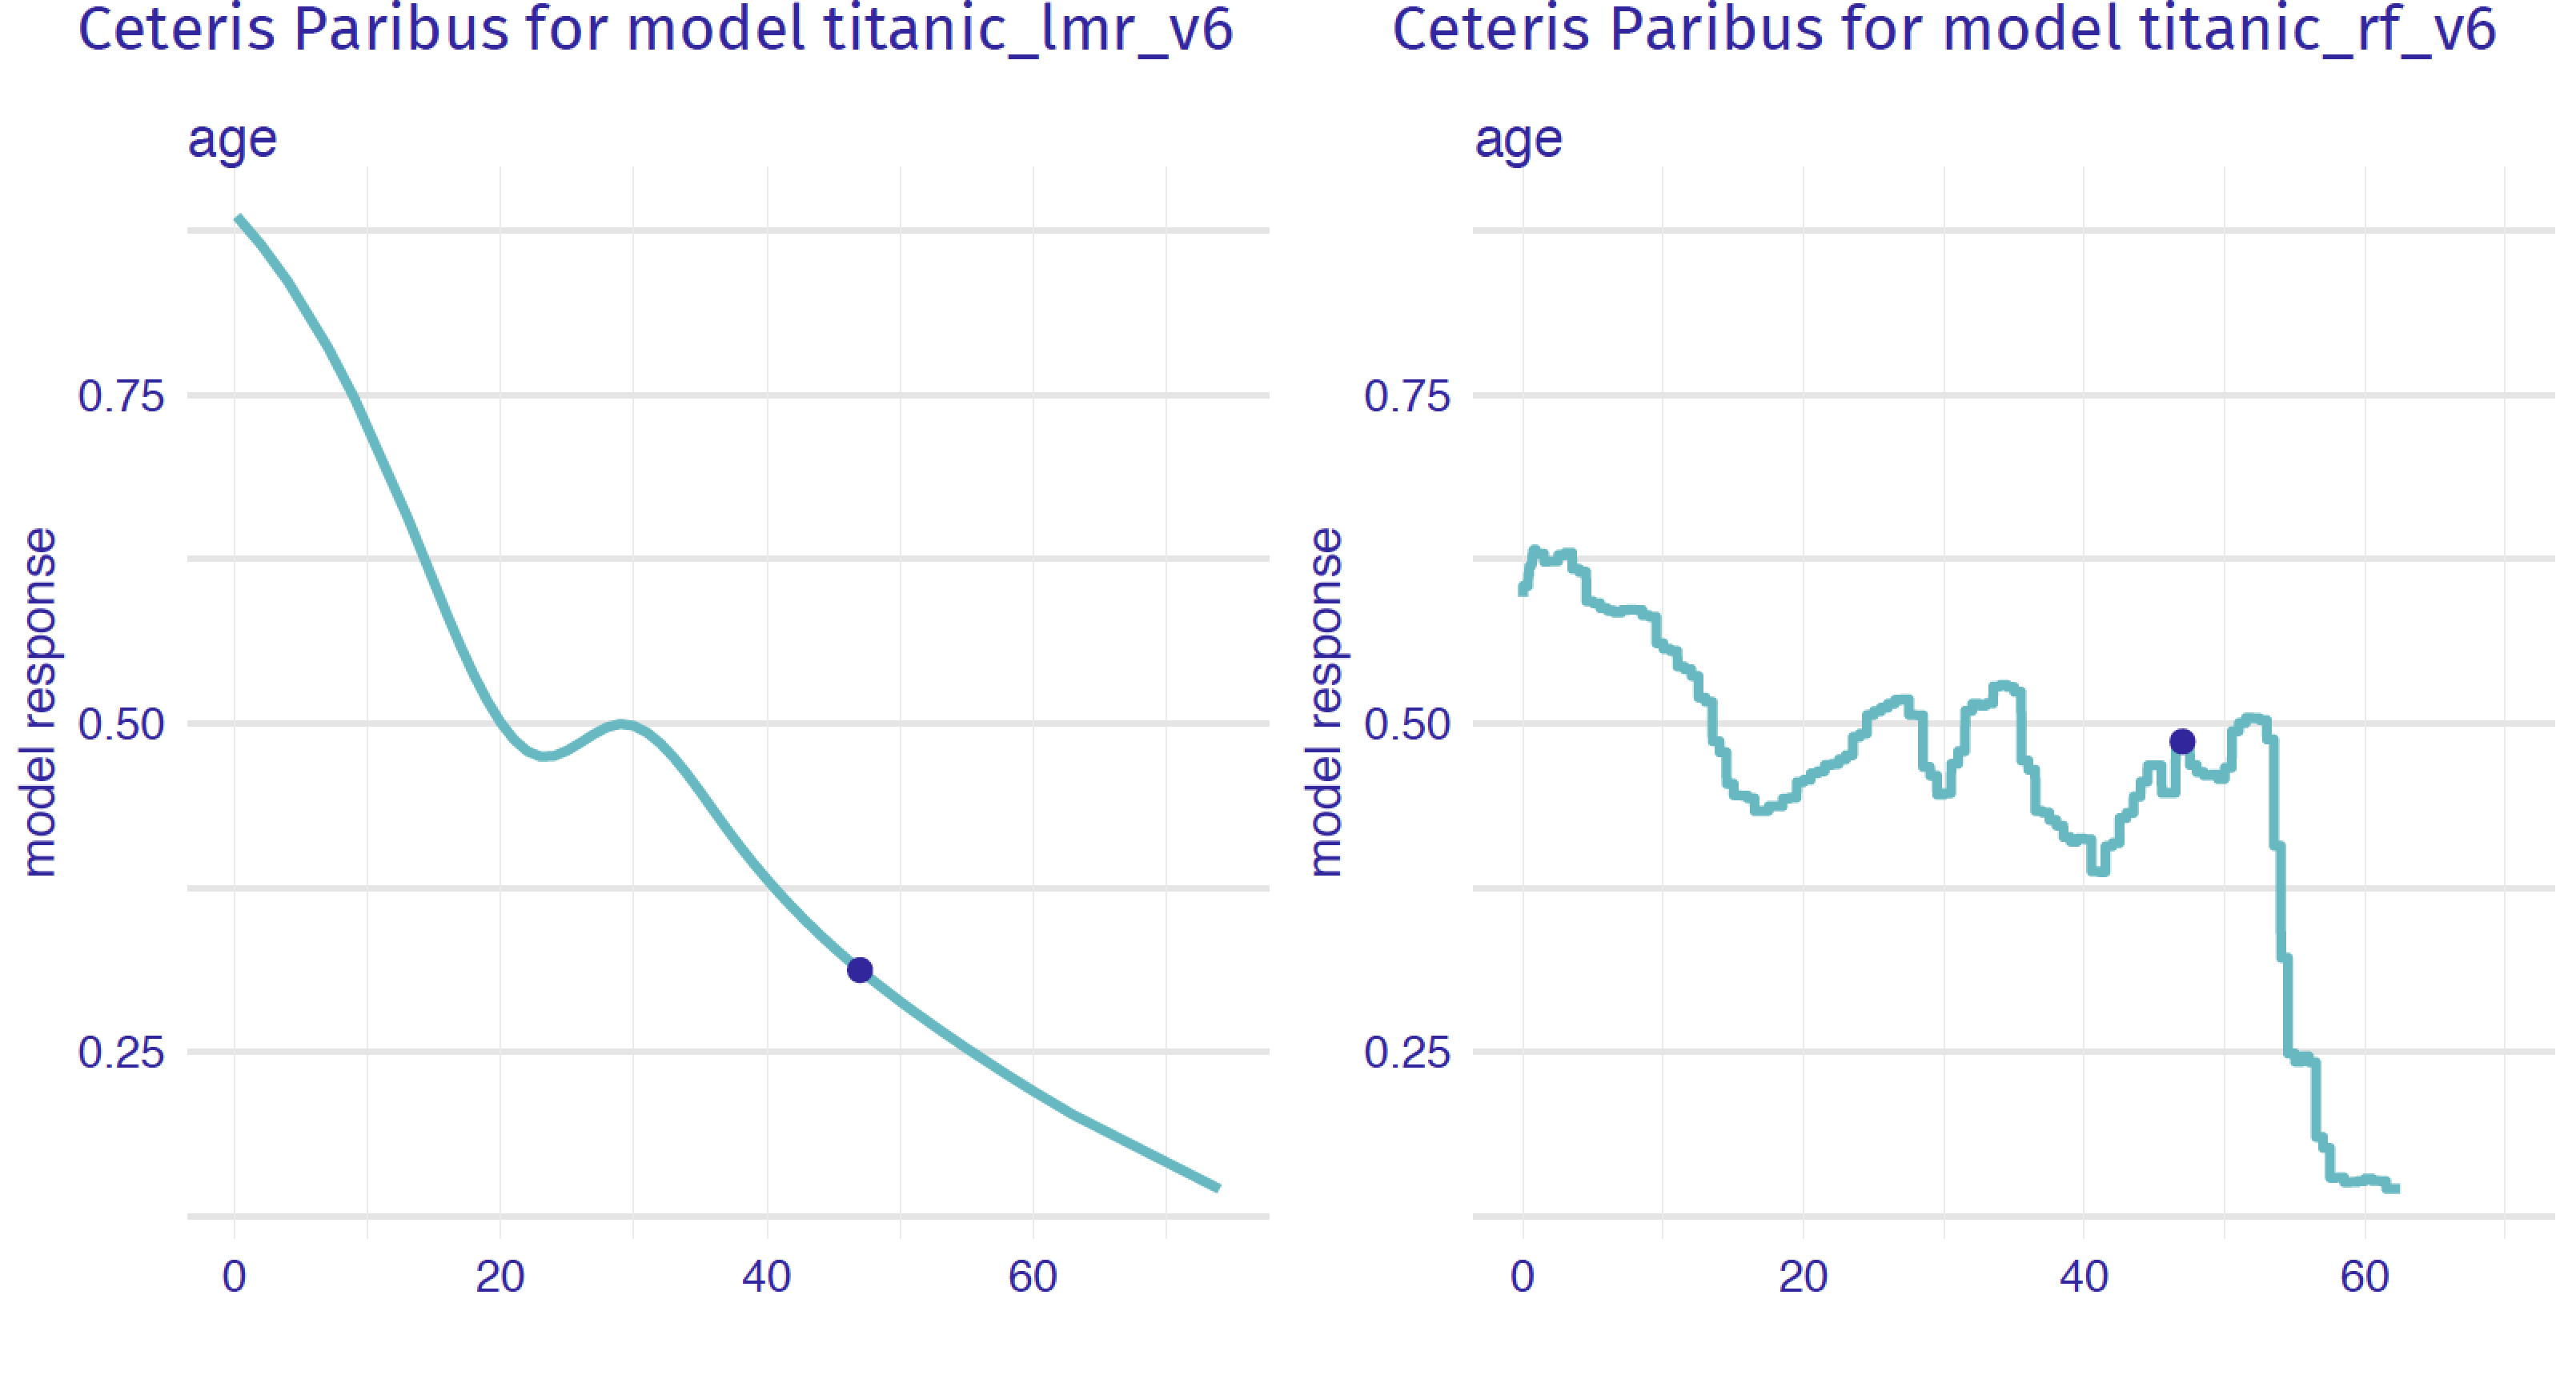
\includegraphics[width=0.7\linewidth]{figure/profile_age_rf}

\}

\textbackslash{}caption\{(fig:profileAgeRf) Ceteris-paribus profiles for variable \texttt{age} for the logistic regression (\texttt{titanic\_lmr\_v6}) and random forest (\texttt{titanic\_rf\_v6} ) models that predict the probability of surviving based on the Titanic data\}\label{fig:profileAgeRf}
\textbackslash{}end\{figure\}

For a categorical explanatory variable, a natural way to represent the CP function is to use a barplot similar to the ones presented in Figure \ref{fig:profileAgeRf2}. The barplots in Figure \ref{fig:profileAgeRf} present CP profiles for the \emph{class} variable in the logistic regression and random forest models for the Titanic dataset (see Sections \ref{model-titanic-lmr} and \ref{model-titanic-rf}, respectively). For this instance (observation), the predicted probability for the logistic regression model would decrease substantially if the value of \emph{class} changed to ``2nd''. On the other hand, for the random forest model, the largest change would be marked if \emph{class} changed to ``restaurant staff''.

\textbackslash{}begin\{figure\}

\{\centering 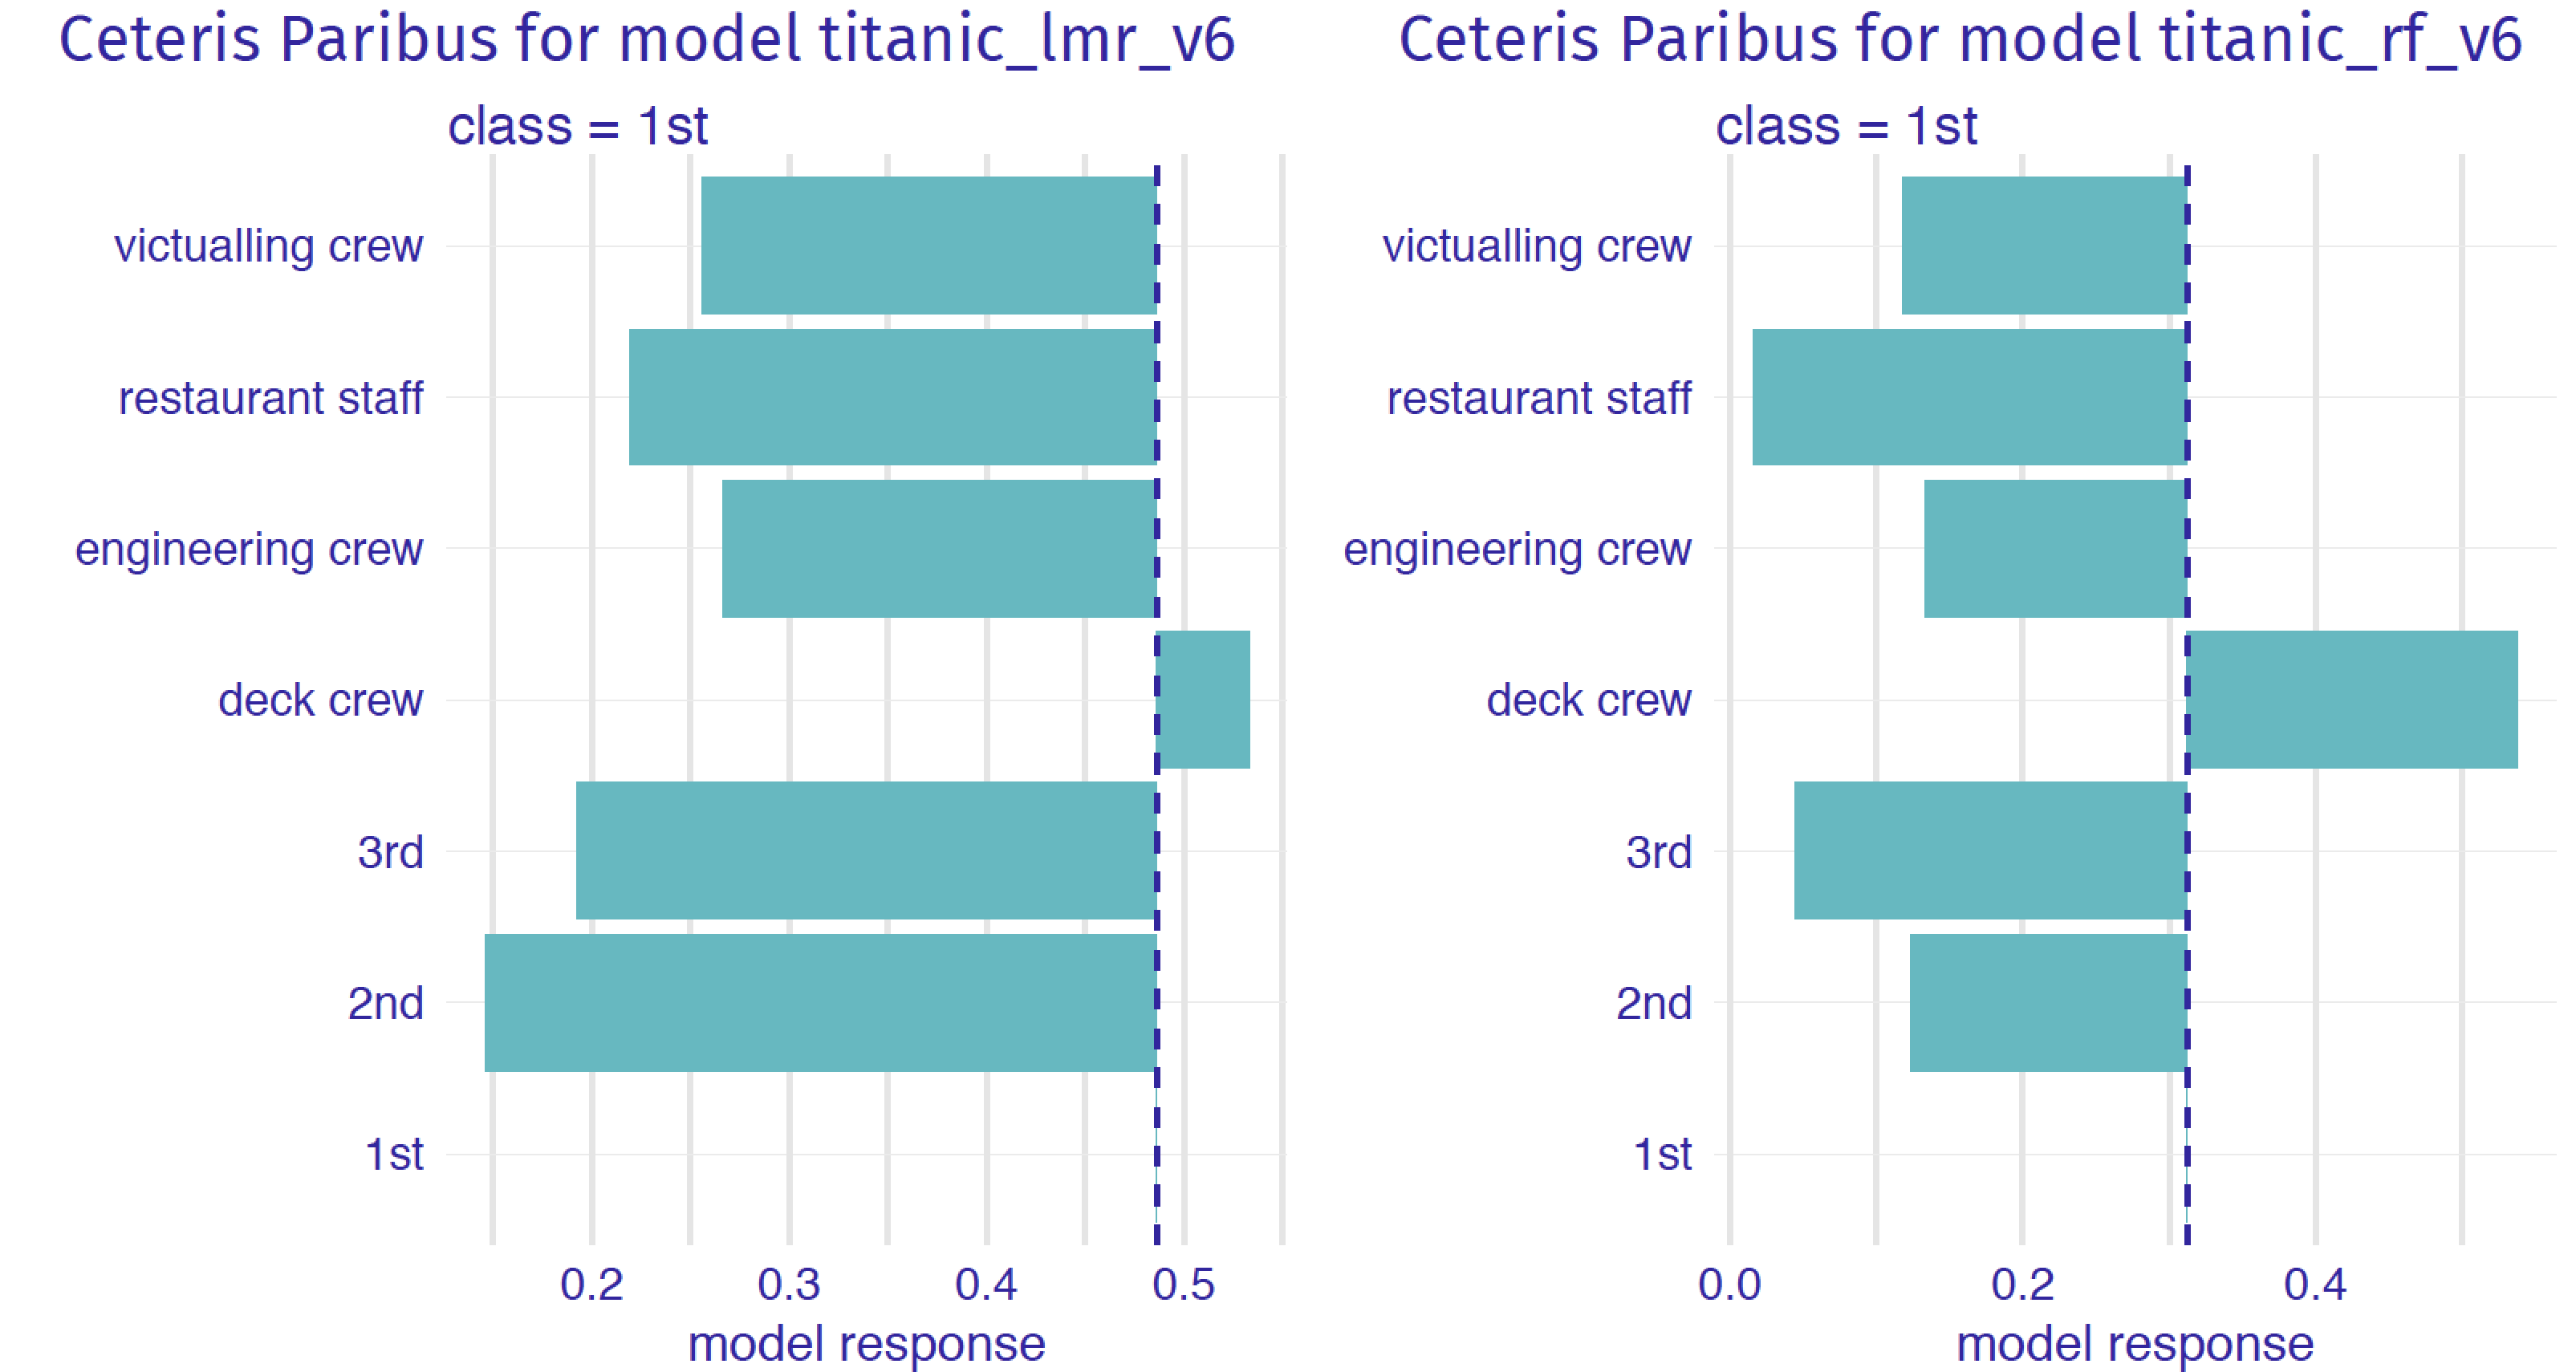
\includegraphics[width=0.7\linewidth]{figure/profile_class_rf}

\}

\textbackslash{}caption\{(fig:profileAgeRf2) Ceteris-paribus profiles for variable \texttt{class} for the logistic regression (\texttt{titanic\_lmr\_v6}) and random forest (\texttt{titanic\_rf\_v6} ) models that predict the probability of surviving based on the Titanic data\}\label{fig:profileAgeRf2}
\textbackslash{}end\{figure\}

Usually, black-box models contain a large number of explanatory variables. However, CP profiles are legible even for tiny subplots, created with techniques like sparklines or small multiples \citep{Tufte1986}. In this way we can display a large number of profiles at the same time keeping profiles for consecutive variables in separate panels, as shown in Figure \ref{fig:profileV4Rf} for the random forest model for the Titanic dataset. It helps if these panels are ordered so that the most important profiles are listed first. We discuss a method to assess the importance of CP profiles in the next chapter.

\textbackslash{}begin\{figure\}

\{\centering 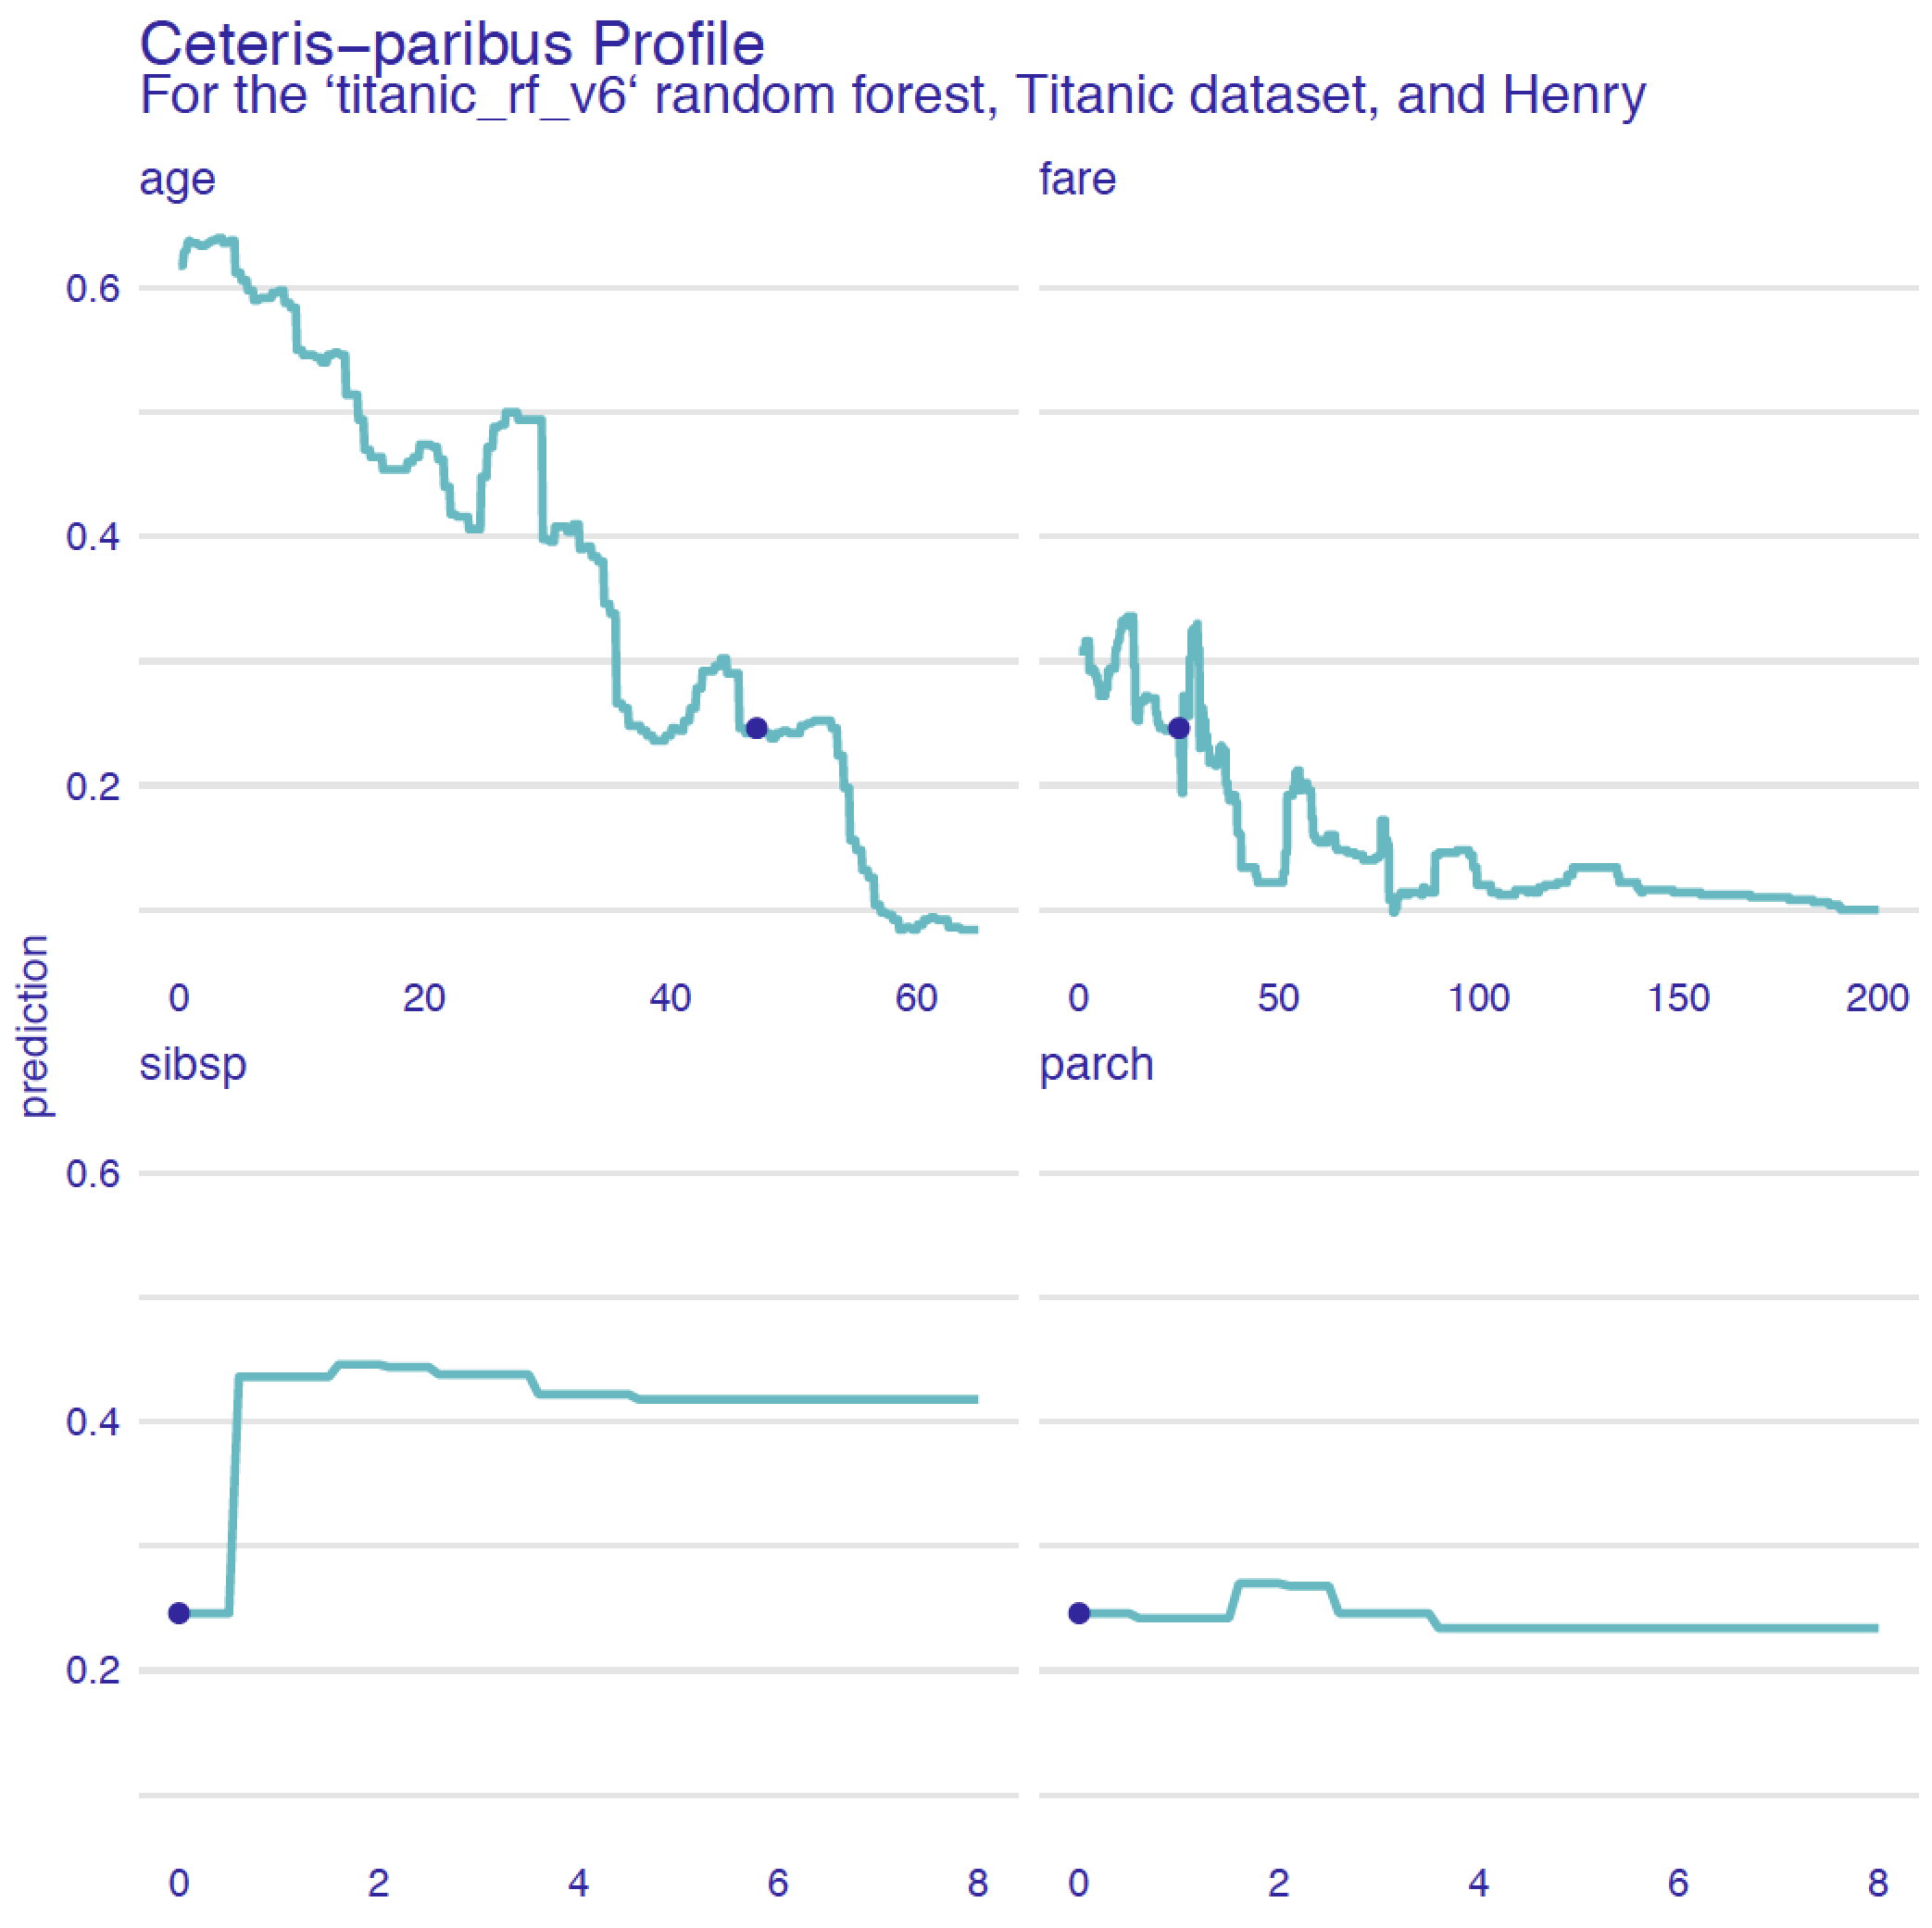
\includegraphics[width=0.7\linewidth]{figure/profile_v4_rf3}

\}

\textbackslash{}caption\{(fig:profileV4Rf) Ceteris-paribus profiles for all continuous explanatory variables for the random forest (\texttt{titanic\_rf\_v6}) model for the \texttt{titanic} dataset\}\label{fig:profileV4Rf}
\textbackslash{}end\{figure\}

\hypertarget{CPProsCons}{%
\subsection{Pros and cons}\label{CPProsCons}}

One-dimensional CP profiles, as presented in this chapter, offer a uniform, easy to communicate and extendable approach to model exploration. Their graphical representation is easy to understand and explain. It is possible to show profiles for many variables or models in a single plot. CP profiles are easy to compare, thus we can juxtapose two or more models to better understand differences between models. We can also compare two or more instances to better understand model stability. CP profiles are also a useful tool for sensitivity analysis.

There are several issues related to the use of the CP profiles. If explanatory variables are correlated, then changing one variable implies a change in the other. In such case, the application of the \emph{Ceteris paribus} principle may lead to unrealistic settings, as it is not possible to keep one variable fixed while varying the other one. For example, apartment's price prediction features like surface and number of rooms are correlated thus it is unrealistic to consider very small apartments with extreme number of rooms. Special cases are interactions, which require the use of two-dimensional CP profiles that are more complex than one-dimensional ones. Also, in case of a model with hundreds or thousands of variables, the number of plots to inspect may be daunting. Finally, while barplots allow visualization of CP profiles for factors (categorical explanatory variables), their use becomes less trivial in case of factors with many nominal (unordered) categories (like, for example, a ZIP-code).

\hypertarget{CPR}{%
\subsection{Code snippets for R}\label{CPR}}

In this section, we present key features of the R package \texttt{ingredients} \citep{ingredientsRPackage} which is a part of \texttt{DrWhy.AI} universe and covers all methods presented in this chapter. More details and examples can be found at \url{https://modeloriented.github.io/ingredients/}.

Note that there are also other R packages that offer similar functionality, like \texttt{condvis} \citep{condvisRPackage}, \texttt{pdp} \citep{pdpRPackage}, \texttt{ICEbox} \citep{ICEbox}, \texttt{ALEPlot} \citep{ALEPlotRPackage}, \texttt{iml} \citep{imlRPackage}.

For illustration, we use two classification models developed in Chapter \ref{TitanicDataset}, namely the logistic regression model \texttt{titanic\_lmr\_v6} (Section \ref{model-titanic-lmr}) and the random forest model \texttt{titanic\_rf\_v6} (Section \ref{model-titanic-rf}). They are developed to predict the probability of survival after sinking of Titanic. Instance-level explanations are calculated for a single observation \texttt{henry} - a 47 years old male passenger that travelled in the 1st class.

\texttt{DALEX} explainers for both models and the \texttt{henry} data frame are retrieved via the \texttt{archivist} hooks as listed in Section \ref{ListOfModelsTitanic}.

\begin{Shaded}
\begin{Highlighting}[]
\KeywordTok{library}\NormalTok{(}\StringTok{"rms"}\NormalTok{)}
\NormalTok{explain_lmr_v6 <-}\StringTok{ }\NormalTok{archivist}\OperatorTok{::}\KeywordTok{aread}\NormalTok{(}\StringTok{"pbiecek/models/2b9b6"}\NormalTok{)}

\KeywordTok{library}\NormalTok{(}\StringTok{"randomForest"}\NormalTok{)}
\NormalTok{explain_rf_v6 <-}\StringTok{ }\NormalTok{archivist}\OperatorTok{::}\KeywordTok{aread}\NormalTok{(}\StringTok{"pbiecek/models/9b971"}\NormalTok{)}

\KeywordTok{library}\NormalTok{(}\StringTok{"DALEX"}\NormalTok{)}
\NormalTok{henry <-}\StringTok{ }\NormalTok{archivist}\OperatorTok{::}\KeywordTok{aread}\NormalTok{(}\StringTok{"pbiecek/models/a6538"}\NormalTok{)}
\NormalTok{henry}
\end{Highlighting}
\end{Shaded}

\begin{verbatim}
##   class gender age sibsp parch fare  embarked
## 1   1st   male  47     0     0   25 Cherbourg
\end{verbatim}

\hypertarget{basic-use-of-the-ceteris_paribus-function}{%
\subsubsection{\texorpdfstring{Basic use of the \texttt{ceteris\_paribus} function}{Basic use of the ceteris\_paribus function}}\label{basic-use-of-the-ceteris_paribus-function}}

The easiest way to create and plot CP profiles is to call \texttt{ceteris\_paribus()} function and then the generic \texttt{plot()} function. By default, profiles for all variables are being calculated and all numeric features are being plotted. One can limit the number of variables that should be considered with the \texttt{variables} argument.

To obtain CP profiles, the \texttt{ceteris\_paribus()} function requires the explainer-object and the instance data frame as arguments. As a result, the function yields an object od the class \texttt{ceteris\_paribus\_explainer}. It is a data frame with model predictions.

\begin{Shaded}
\begin{Highlighting}[]
\KeywordTok{library}\NormalTok{(}\StringTok{"ingredients"}\NormalTok{)}
\NormalTok{cp_titanic_rf <-}\StringTok{ }\KeywordTok{ceteris_paribus}\NormalTok{(explain_rf_v6, henry)}
\NormalTok{cp_titanic_rf}
\end{Highlighting}
\end{Shaded}

\begin{verbatim}
## Top profiles    : 
##                class gender age sibsp parch fare  embarked _yhat_ _vname_ _ids_
## 1                1st   male  47     0     0   25 Cherbourg  0.246   class     1
## 1.1              2nd   male  47     0     0   25 Cherbourg  0.054   class     1
## 1.2              3rd   male  47     0     0   25 Cherbourg  0.100   class     1
## 1.3        deck crew   male  47     0     0   25 Cherbourg  0.454   class     1
## 1.4 engineering crew   male  47     0     0   25 Cherbourg  0.096   class     1
## 1.5 restaurant staff   male  47     0     0   25 Cherbourg  0.092   class     1
##              _label_
## 1   Random Forest v6
## 1.1 Random Forest v6
## 1.2 Random Forest v6
## 1.3 Random Forest v6
## 1.4 Random Forest v6
## 1.5 Random Forest v6
## 
## 
## Top observations:
##   class gender age sibsp parch fare  embarked _yhat_          _label_ _ids_
## 1   1st   male  47     0     0   25 Cherbourg  0.246 Random Forest v6     1
\end{verbatim}

To obtain a graphical representation of CP profiles, the generic \texttt{plot()} function can be applied to the data frame returned by the \texttt{ceteris\_paribus()} function. It returns a \texttt{ggplot2} object that can be processed further if needed. In the examples below, we use the \texttt{ggplot2} functions, like \texttt{ggtitle()} or \texttt{ylim()}, to modify plot's title or the range of the Y-axis.

The resulting plot can be enriched with additional data by applying functions \texttt{ingredients::show\_rugs} (adds rugs for the selected points), \texttt{ingredients::show\_observations} (adds dots that shows observations), or \texttt{ingredients::show\_aggreagated\_profiles}. All these functions can take additional arguments to modify size, color, or linetype.

Below we show an R snippet that can be used to replicate plots presented in the upper part of Figure \ref{fig:profileV4Rf}.

\begin{Shaded}
\begin{Highlighting}[]
\KeywordTok{library}\NormalTok{(}\StringTok{"ggplot2"}\NormalTok{)}
\KeywordTok{plot}\NormalTok{(cp_titanic_rf, }\DataTypeTok{variables =} \KeywordTok{c}\NormalTok{(}\StringTok{"age"}\NormalTok{, }\StringTok{"fare"}\NormalTok{)) }\OperatorTok{+}
\StringTok{  }\KeywordTok{show_observations}\NormalTok{(cp_titanic_rf, }\DataTypeTok{variables =} \KeywordTok{c}\NormalTok{(}\StringTok{"age"}\NormalTok{, }\StringTok{"fare"}\NormalTok{)) }\OperatorTok{+}
\StringTok{  }\KeywordTok{ggtitle}\NormalTok{(}\StringTok{"Ceteris Paribus Profiles"}\NormalTok{, }\StringTok{"For the random forest model and the Titanic dataset"}\NormalTok{)}
\end{Highlighting}
\end{Shaded}

\textbackslash{}begin\{figure\}

\{\centering 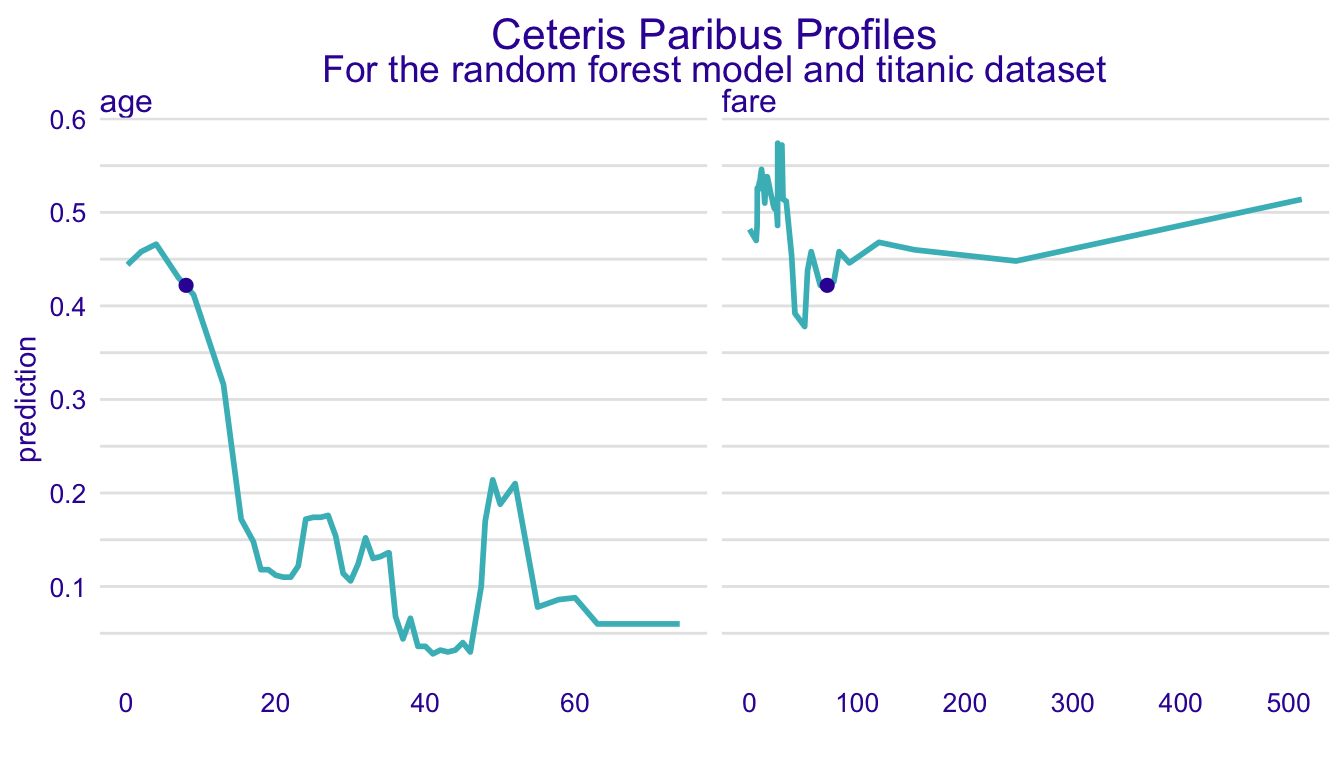
\includegraphics[width=0.7\linewidth]{PM_VEE_files/figure-latex/titanicCeterisProfile01-1}

\}

\textbackslash{}caption\{Ceteris-paribus profiles for \texttt{age} and \texttt{fare} variables and the \texttt{titanic\_rf\_v6} model.\}\label{fig:titanicCeterisProfile01}
\textbackslash{}end\{figure\}

By default, all numerical variables are plotted.
To plot CP profiles for categorical variables, we have got to add the \texttt{only\_numerical\ =\ FALSE} argument to the \texttt{plot()} function. The code below an be used to recreate the right-hand-side plot from Figure \ref{fig:profileAgeRf2}.

\begin{Shaded}
\begin{Highlighting}[]
\KeywordTok{plot}\NormalTok{(cp_titanic_rf, }\DataTypeTok{variables =} \KeywordTok{c}\NormalTok{(}\StringTok{"class"}\NormalTok{, }\StringTok{"embarked"}\NormalTok{), }\DataTypeTok{only_numerical =} \OtherTok{FALSE}\NormalTok{) }\OperatorTok{+}
\StringTok{  }\KeywordTok{ggtitle}\NormalTok{(}\StringTok{"Ceteris Paribus Profiles"}\NormalTok{, }\StringTok{"For the random forest model and the Titanic dataset"}\NormalTok{)}
\end{Highlighting}
\end{Shaded}

\textbackslash{}begin\{figure\}

\{\centering 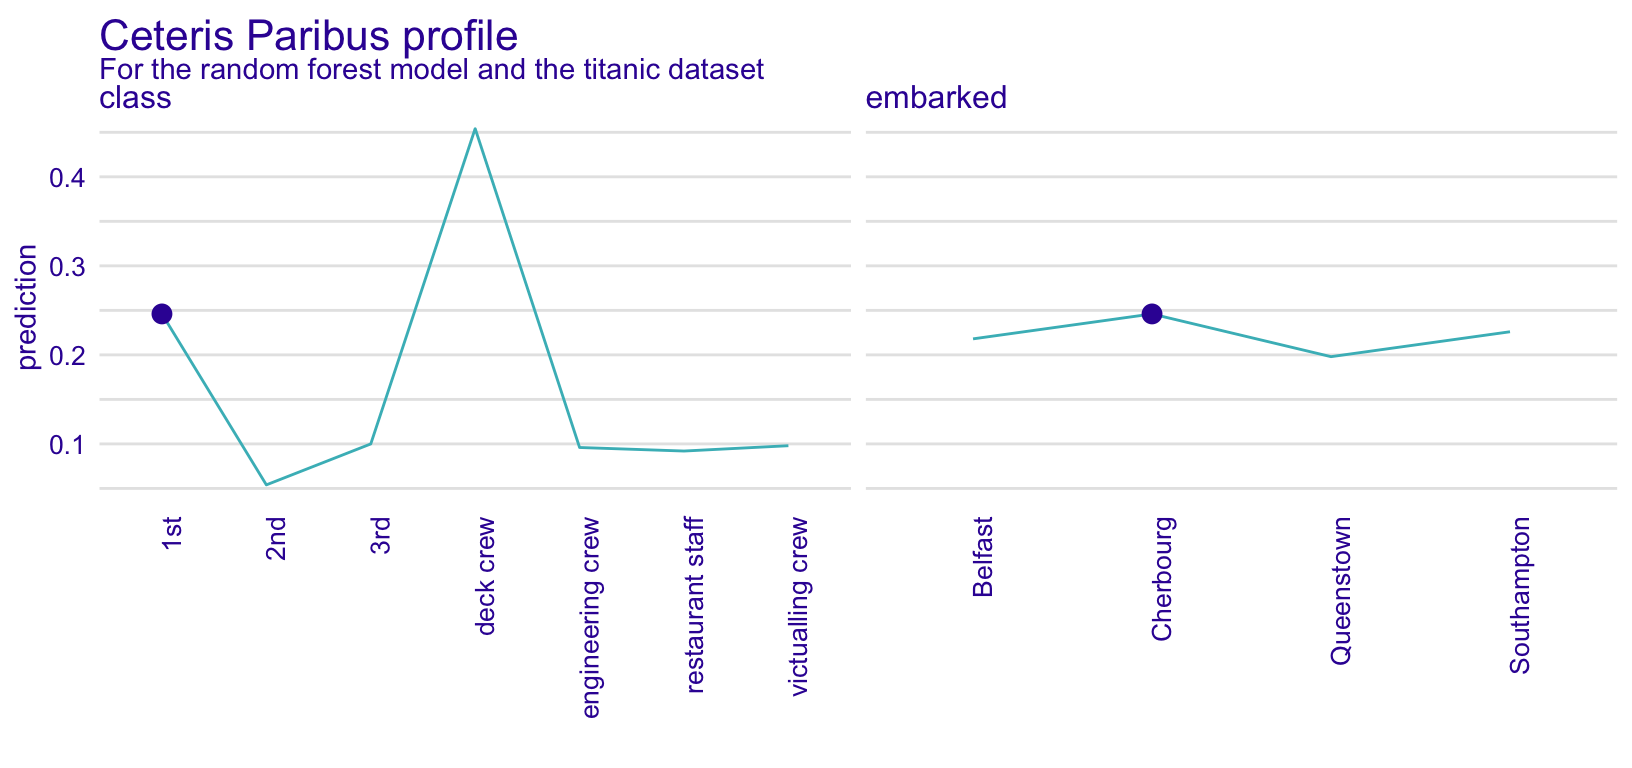
\includegraphics[width=0.7\linewidth]{PM_VEE_files/figure-latex/titanicCeterisProfile01B-1}

\}

\textbackslash{}caption\{Ceteris-paribus profiles for \texttt{class} and \texttt{embarked} variables and the \texttt{titanic\_rf\_v6} model.\}\label{fig:titanicCeterisProfile01B}
\textbackslash{}end\{figure\}

\hypertarget{advanced-use-of-the-ceteris_paribus-function}{%
\subsubsection{\texorpdfstring{Advanced use of the \texttt{ceteris\_paribus} function}{Advanced use of the ceteris\_paribus function}}\label{advanced-use-of-the-ceteris_paribus-function}}

The \texttt{ceteris\_paribus()} is a very flexible function. To better understand how it can be used, we briefly review its arguments.

\begin{itemize}
\tightlist
\item
  \texttt{x}, \texttt{data}, \texttt{predict\_function}, \texttt{label} - information about a model. If \texttt{x} is created with the \texttt{DALEX::explain} function, then other arguments are extracted from \texttt{x}; this is how we use the function in this chapter. Otherwise, we have got to specify directly the model, the validation data, the predict function, and the model label.
\item
  \texttt{new\_observation} - instance (one or more), for which we want to calculate CP profiles. It should be a data frame with same variables as in the validation data.
\item
  \texttt{y} - observed value of the dependent variable for \texttt{new\_observation}. The use of this argument is illustrated in Section \ref{cPLocDiagIntro}.
\item
  \texttt{variables} - names of explanatory variables, for which CP profiles are to be calculated. By default, the profiles will be constructed for all variables, which may be time consuming.
\item
  \texttt{variable\_splits} - a list of values for which CP profiles are to be calculated. By default, these are all values for categorical variables. For continuous variables, uniformly-placed values are selected; one can specify the number of the values with the \texttt{grid\_points} argument (the default is 101).
\end{itemize}

The code below allows to obtain the plots in the upper part of Figure \ref{fig:profileV4Rf}. The argument \texttt{variable\_splits} specifies the variables (\texttt{age} and \texttt{fare}) for which CP profiles are to be calculated, together with the list of values at which the profiles are to be evaluated.

\begin{Shaded}
\begin{Highlighting}[]
\NormalTok{cp_titanic_rf <-}\StringTok{ }\KeywordTok{ceteris_paribus}\NormalTok{(explain_rf_v6, henry,}
              \DataTypeTok{variable_splits =} \KeywordTok{list}\NormalTok{(}\DataTypeTok{age =} \KeywordTok{seq}\NormalTok{(}\DecValTok{0}\NormalTok{, }\DecValTok{70}\NormalTok{, }\FloatTok{0.1}\NormalTok{),}
                                     \DataTypeTok{fare =} \KeywordTok{seq}\NormalTok{(}\DecValTok{0}\NormalTok{, }\DecValTok{100}\NormalTok{, }\FloatTok{0.1}\NormalTok{)))}
\end{Highlighting}
\end{Shaded}

\begin{Shaded}
\begin{Highlighting}[]
\KeywordTok{plot}\NormalTok{(cp_titanic_rf) }\OperatorTok{+}\StringTok{ }
\StringTok{  }\KeywordTok{show_observations}\NormalTok{(cp_titanic_rf, }\DataTypeTok{variables =} \KeywordTok{c}\NormalTok{(}\StringTok{"age"}\NormalTok{, }\StringTok{"fare"}\NormalTok{), }\DataTypeTok{size =} \DecValTok{5}\NormalTok{) }\OperatorTok{+}\StringTok{ }
\StringTok{  }\KeywordTok{ylim}\NormalTok{(}\DecValTok{0}\NormalTok{, }\DecValTok{1}\NormalTok{) }\OperatorTok{+}
\StringTok{  }\KeywordTok{ggtitle}\NormalTok{(}\StringTok{"Ceteris Paribus Profiles"}\NormalTok{, }\StringTok{"For the random forest model and titanic dataset"}\NormalTok{)}
\end{Highlighting}
\end{Shaded}

\textbackslash{}begin\{figure\}

\{\centering 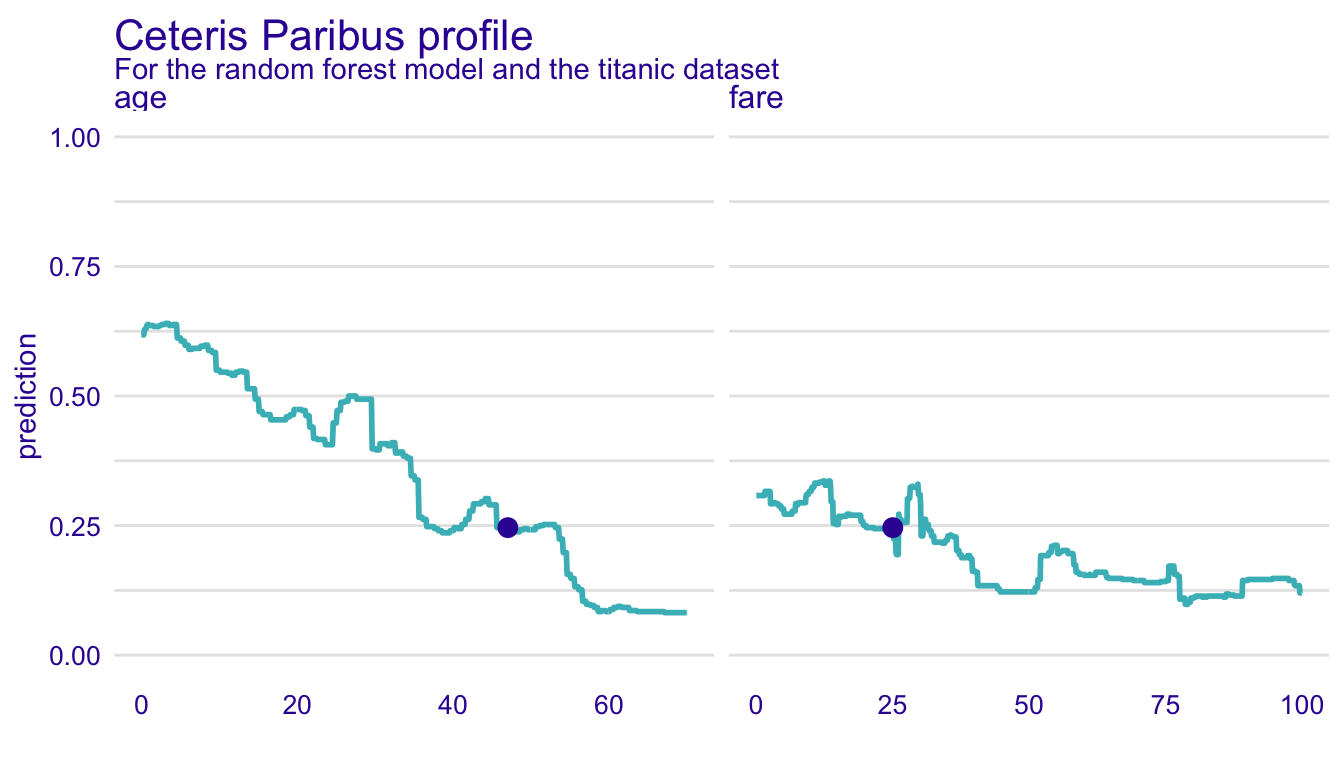
\includegraphics[width=0.7\linewidth]{PM_VEE_files/figure-latex/titanicCeterisProfile01C-1}

\}

\textbackslash{}caption\{Ceteris-paribus profiles for \texttt{class} and \texttt{embarked} variables and the \texttt{titanic\_rf\_v6} model. Blue dot stands for \texttt{henry}.\}\label{fig:titanicCeterisProfile01C}
\textbackslash{}end\{figure\}

To enhance the plot, additional functions can be used. The generic \texttt{plot()} function creates a \texttt{ggplot2} object with a single \texttt{geom\_line} layer. Function \texttt{show\_observations} adds \texttt{geom\_point} layer, \texttt{show\_rugs} adds \texttt{geom\_rugs}, while \texttt{show\_profiles} adds another \texttt{geom\_line}. All these functions take, as the first argument, an object created with the \texttt{ceteris\_paribus} function. They can be combined freely to superpose profiles for different models or observations.

In the example below, we present the code to create XO profiles for two passengers, \texttt{henry} and \texttt{johny\_d}. Their profiles are included in a plot presented in Figure \ref{fig:titanicCeterisProfile01D}. We use the \texttt{scale\_color\_manual} function to add names of passengers to the plot, and to control colors and positions.

\begin{Shaded}
\begin{Highlighting}[]
\NormalTok{johny_d <-}\StringTok{ }\NormalTok{archivist}\OperatorTok{::}\KeywordTok{aread}\NormalTok{(}\StringTok{"pbiecek/models/e3596"}\NormalTok{)}
\NormalTok{cp_titanic_rf2 <-}\StringTok{ }\KeywordTok{ceteris_paribus}\NormalTok{(explain_rf_v6, }\KeywordTok{rbind}\NormalTok{(henry, johny_d))}
\end{Highlighting}
\end{Shaded}

\begin{Shaded}
\begin{Highlighting}[]
\KeywordTok{plot}\NormalTok{(cp_titanic_rf2, }\DataTypeTok{color =} \StringTok{"_ids_"}\NormalTok{) }\OperatorTok{+}\StringTok{ }
\StringTok{  }\KeywordTok{show_observations}\NormalTok{(cp_titanic_rf2, }\DataTypeTok{size =} \DecValTok{5}\NormalTok{, }\DataTypeTok{variables =} \KeywordTok{c}\NormalTok{(}\StringTok{"age"}\NormalTok{, }\StringTok{"fare"}\NormalTok{)) }\OperatorTok{+}\StringTok{ }
\StringTok{  }\KeywordTok{show_rugs}\NormalTok{(cp_titanic_rf2, }\DataTypeTok{sides =} \StringTok{"bl"}\NormalTok{, }\DataTypeTok{variables =} \KeywordTok{c}\NormalTok{(}\StringTok{"age"}\NormalTok{, }\StringTok{"fare"}\NormalTok{)) }\OperatorTok{+}\StringTok{ }
\StringTok{  }\KeywordTok{scale_color_manual}\NormalTok{(}\DataTypeTok{name =} \StringTok{"Passenger:"}\NormalTok{, }\DataTypeTok{breaks =} \DecValTok{1}\OperatorTok{:}\DecValTok{2}\NormalTok{, }\DataTypeTok{values =} \KeywordTok{c}\NormalTok{(}\StringTok{"#4378bf"}\NormalTok{, }\StringTok{"#8bdcbe"}\NormalTok{), }\DataTypeTok{labels =} \KeywordTok{c}\NormalTok{(}\StringTok{"henry"}\NormalTok{ , }\StringTok{"johny_d"}\NormalTok{)) }\OperatorTok{+}\StringTok{ }
\StringTok{  }\KeywordTok{ggtitle}\NormalTok{(}\StringTok{"Ceteris Paribus Profiles"}\NormalTok{, }\StringTok{"For the random forest model and the Titanic dataset"}\NormalTok{)}
\end{Highlighting}
\end{Shaded}

\textbackslash{}begin\{figure\}

\{\centering 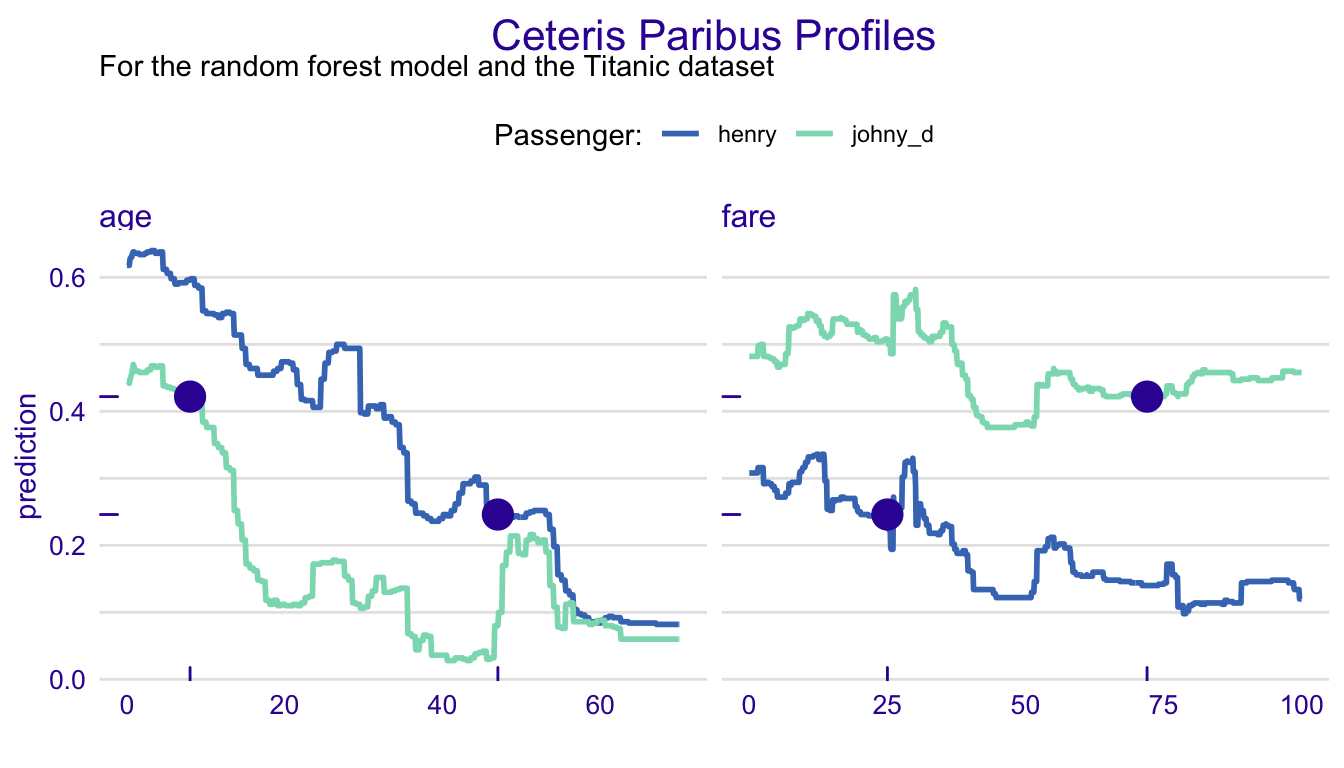
\includegraphics[width=0.7\linewidth]{PM_VEE_files/figure-latex/titanicCeterisProfile01D-1}

\}

\textbackslash{}caption\{Ceteris-paribus profiles for the \texttt{titanic\_rf\_v6} model. Profiles for different passangers are color-coded.\}\label{fig:titanicCeterisProfile01D}
\textbackslash{}end\{figure\}

\hypertarget{champion-challenger-analysis}{%
\subsubsection{Champion-challenger analysis}\label{champion-challenger-analysis}}

One of the most interesting uses of the explainers is comparison of CP profiles for two or more of models.

To illustrate this possibility, first, we have go to construct profiles for the models. In our illustration, for the sake of clarity, we limit ourselves just to two models: the logistic regression and random forest models for the Titanic data. Moreover, we only consider the \texttt{age} and \texttt{fare} variables. We use \texttt{henry} as the instance, for which predictions are of interest.

\begin{Shaded}
\begin{Highlighting}[]
\NormalTok{cp_titanic_rf <-}\StringTok{ }\KeywordTok{ceteris_paribus}\NormalTok{(explain_rf_v6, henry)}
\NormalTok{cp_titanic_lmr <-}\StringTok{ }\KeywordTok{ceteris_paribus}\NormalTok{(explain_lmr_v6, henry)}
\end{Highlighting}
\end{Shaded}

Subsequently, we construct the plot. The result is shown in Figure \ref{fig:titanicCeterisProfile01E}. Predictions for \texttt{henry} are slightly different, logistic regression returns in this case higher predictions then random forest. For \texttt{age} variable profiles of both models are similar, in both models we see decreasing dependency. While for \texttt{fare} the logistic regression model is slightly positive while random forest is negative. The larger the \texttt{fare} the larger is difference between these models. Such analysis helps us to which degree different models agree on what if scenarios.

Note that every \texttt{plot} and \texttt{show\_*} function can take a collection of explainers as arguments. Profiles for different models are included in a single plot. In the presented R snippet, models are color-coded with the help of the argument \texttt{color\ =\ "\_label\_"}, where \texttt{\_label\_} refers to the name of the column in the CP explainer that contains the model label.

\begin{Shaded}
\begin{Highlighting}[]
\KeywordTok{plot}\NormalTok{(cp_titanic_rf, cp_titanic_lmr, }\DataTypeTok{color =} \StringTok{"_label_"}\NormalTok{) }\OperatorTok{+}
\StringTok{  }\KeywordTok{show_observations}\NormalTok{(cp_titanic_rf, cp_titanic_lmr, }\DataTypeTok{color =} \StringTok{"black"}\NormalTok{, }\DataTypeTok{variables =} \KeywordTok{c}\NormalTok{(}\StringTok{"age"}\NormalTok{, }\StringTok{"fare"}\NormalTok{), }\DataTypeTok{size =} \DecValTok{5}\NormalTok{) }\OperatorTok{+}
\StringTok{  }\KeywordTok{scale_color_discrete}\NormalTok{(}\DataTypeTok{name =} \StringTok{"Selected models:"}\NormalTok{) }\OperatorTok{+}\StringTok{ }\KeywordTok{ylim}\NormalTok{(}\DecValTok{0}\NormalTok{,}\DecValTok{1}\NormalTok{) }\OperatorTok{+}\StringTok{ }
\StringTok{  }\KeywordTok{ggtitle}\NormalTok{(}\StringTok{"Ceteris Paribus Profiles for Henry"}\NormalTok{)}
\end{Highlighting}
\end{Shaded}

\textbackslash{}begin\{figure\}

\{\centering 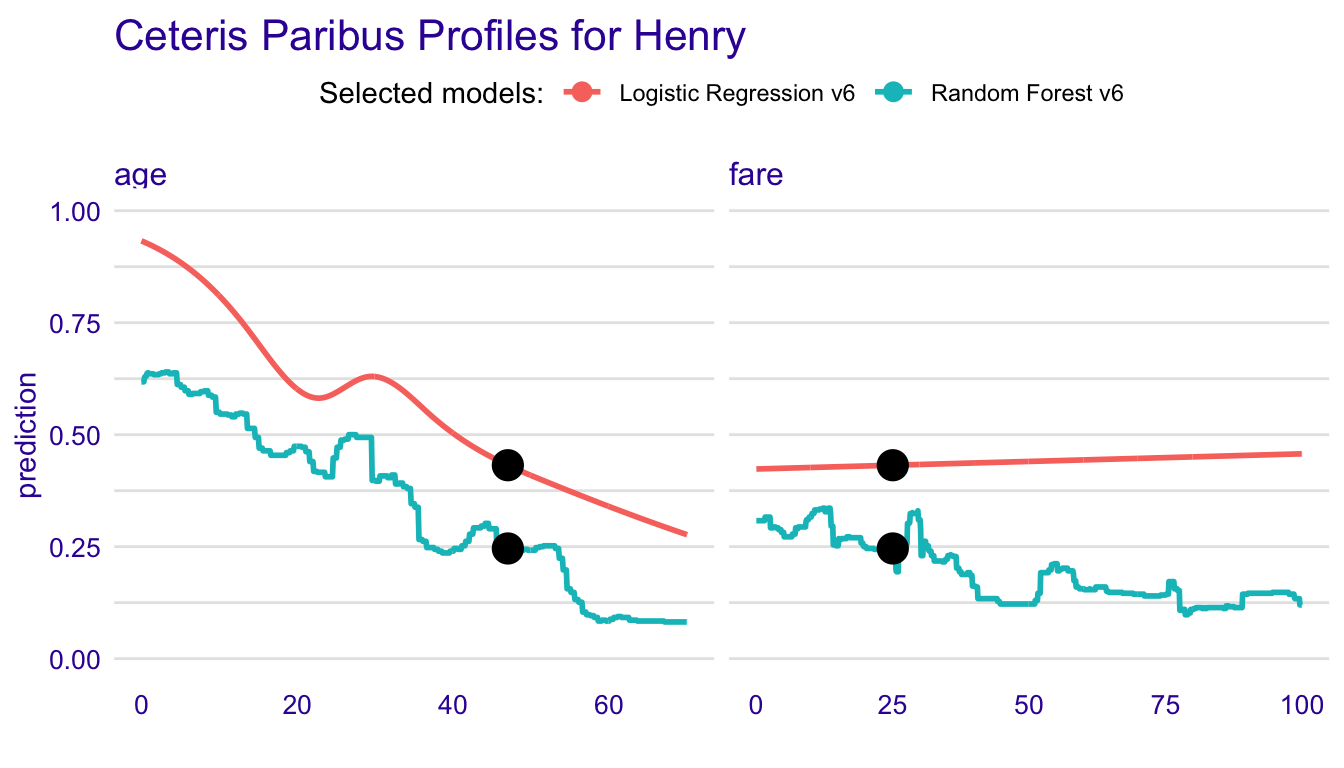
\includegraphics[width=0.7\linewidth]{PM_VEE_files/figure-latex/titanicCeterisProfile01E-1}

\}

\textbackslash{}caption\{Champion-challenger comparison of the \texttt{titanic\_lmr\_v6} and \texttt{titanic\_rf\_v6} models. Profiles for different models are color-coded.\}\label{fig:titanicCeterisProfile01E}
\textbackslash{}end\{figure\}

\hypertarget{ceterisParibusOscillations}{%
\section{Ceteris-paribus Oscillations and Local Variable-importance}\label{ceterisParibusOscillations}}

\hypertarget{CPOscIntro}{%
\subsection{Introduction}\label{CPOscIntro}}

Visual examination of Ceteris-paribus (CP) profiles is insightful, but for a model with a large number of explanatory variables we may end up with a large number of plots which may be overwhelming. To prioritize between the profiles we need a measure that would summarize the impact of a selected variable on model's predictions. In this chapter we describe a solution closely linked with CP profiles. An alternative is discussed in the Chapters \ref{breakDown} and \ref{shapley}.

\hypertarget{CPOscIntuition}{%
\subsection{Intuition}\label{CPOscIntuition}}

To assign importance to CP profiles, we can use the concept of profile oscillations. In particular, the larger influence of an explanatory variable on prediction at a particular instance, the larger the fluctuations along the corresponding CP profile. For a variable that exercises little or no influence on model prediction, the profile will be flat or will barely change. In other words, the values of the CP profile should be close to the value of the model prediction for the particular instance. Consequently, the sum of differences between the profile and the value of the prediction, take across all possible values of the explanatory variable, should be close to zero. The sum can be graphically depicted by the area between the profile and the horizontal line representing the instance prediction. On the other hand, for an explanatory variable with a large influence on the prediction, the area should be large. Figure \ref{fig:CPVIPprofiles} illustrates the concept. Panle A of the figure corresponds to the CP profiles presented in Figure \ref{fig:profileV4Rf}. The larger the highlighted area in Figure \ref{fig:CPVIPprofiles}, the more important is the variable for the particular prediction.

\textbackslash{}begin\{figure\}

\{\centering 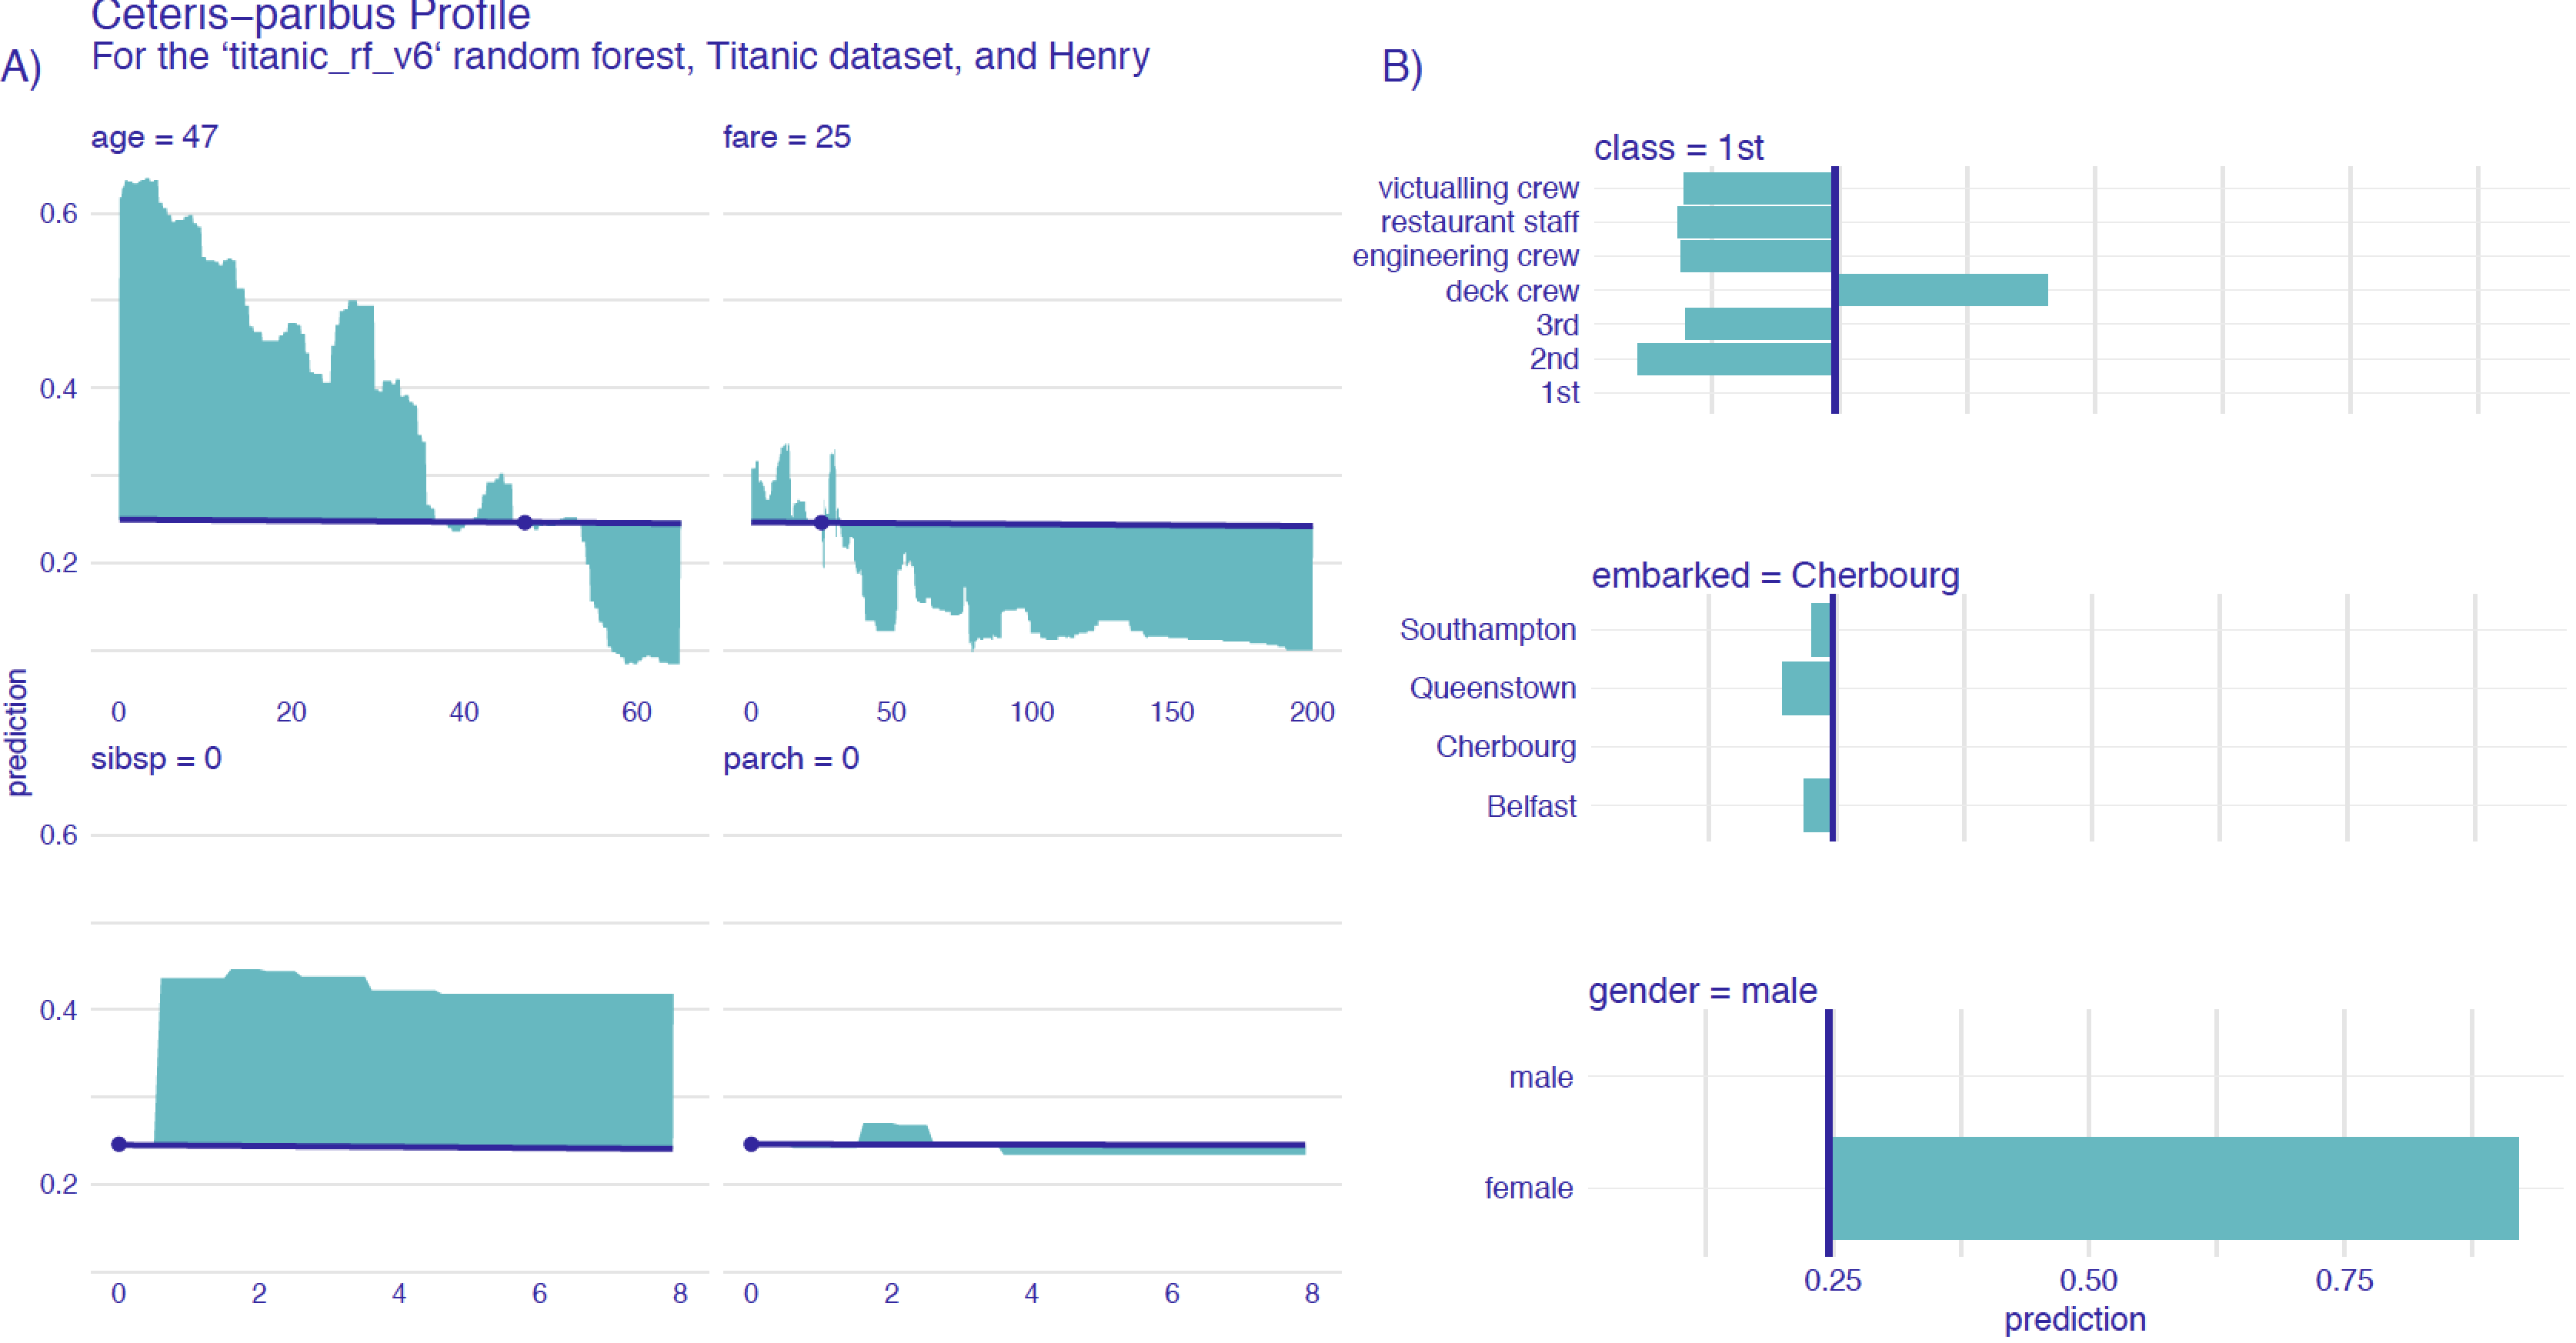
\includegraphics[width=0.99\linewidth]{figure/profile_v4_rf2}

\}

\textbackslash{}caption\{(fig:CPVIPprofiles) The value of the colored area summarizes the Ceteris-paribus-profile oscillations and provides the mean of the absolute deviations between the CP profile and the instance prediction. Panel A shows plots for continuous explanatory variables, while panel B shows plots for categorical variables in the \texttt{titanic\_rf\_v6} model.\}\label{fig:CPVIPprofiles}
\textbackslash{}end\{figure\}

\hypertarget{CPOscMethod}{%
\subsection{Method}\label{CPOscMethod}}

Let us formalize this concept now. Denote by \(g^j(z)\) the probability density function of the distribution of the \(j\)-th explanatory variable. The summary measure of the variable's importance for model prediction at point \(x_*\), \(vip_{CP}^{j}(x_*)\), computed based on the variable's CP profile, is defined as follows:

\begin{equation}
vip_{CP}^j(x_*) = \int_{\mathcal R} |h^{j}_{x_*}(z) - f(x_*)| g^j(z)dz=E_{X^j}\left[|h^{j}_{x_*}(X^j) - f(x_*)|\right].
\label{eq:VIPCPdef}
\end{equation}

Thus, \(vip_{CP}^j(x_*)\) is the expected absolute deviation of the CP profile from the model prediction for \(x_*\) over the distribution \(g^j(z)\) for the \(j\)-th explanatory variable.

The true distribution of \(j\)-th explanatory variable is, in most cases, unknown. Thus, there are several options how to calculate \eqref{eq:VIPCPdef}.

One is to calculate just the area under the CP curve, i.e., to assume that \(g^j(z)\) is a uniform distribution for the range of variable \(x^j\). It folows then that a straightforward estimator of \(vip_{CP}^{j,uni}(x_*)\) is

\begin{equation}
\widehat{vip}_{CP}^{j,uni}(x_*) = \frac 1k \sum_{l=1}^k |h^{j}_{x_*}(z_l) - f(x_*)|,
\label{eq:VIPCPuni}
\end{equation}

where \(z_l\) (\(l=1, \ldots, k\)) are the selected values of the \(j\)-th explanatory variable. For instance, one can select use all unique values of \(x^{j}\) in the considered dataset. Alternatively, for a continuous variable, one can use an equi-distant grid of values.

Another approach is to use the empirical distribution for \(x^{j}\). This leads to the estimator of \(vip_{CP}^{j,emp}(x_*)\) defined as

\begin{equation}
\widehat{vip}_{CP}^{j,emp}(x_*) = \frac 1n \sum_{i=1}^n |h^{j}_{x_*}(x^{j}_i) - f(x_*)|,
\label{eq:VIPCPemp}
\end{equation}

where index \(i\) goes through all observations in a dataset.

The use of of \(\widehat{vip}_{CP}^{j,emp}(x_*)\) is preferred when there are enough data to accurately estimate the empirical distribution and when the distribution is not uniform. On the other hand, \(\widehat{vip}_{CP}^{j,uni}(x_*)\) is in most cases quicker to compute and, therefore, it is preferred if we look for fast approximations.

It is worth noting that the importance of an explanatory variable for instance prediction may be very different for different points \(x_*\). For example, consider model
\[
f(x_1, x_2) = x_1 * x_2,
\]
where \(x_1\) and \(x_2\) take values in \([0,1]\). Consider prediction for an observation described by vector \(x_* = (0,1)\). In that case, the importance of \(X_1\) is larger than \(X_2\). This is because the CP profile for the first variable, given by the values of function \(f(z,1)=z\), will have oscillations. On the other hand, the profile for the second variable will show no oscillations, because the profile is given by function \(f(0,z)=0\). Obviously, the situation is reversed for \(x_*=(1,0)\).

\hypertarget{CPOscExample}{%
\subsection{Example: Titanic}\label{CPOscExample}}

Figure \ref{fig:CPVIP1} provides a barplot of variable importance measures for different continuous explanatory variables for the random forest model \texttt{titanic\_rf\_v6} for \texttt{henry}.

The longer the bar, the larger the CP-profile oscillations for a particular explanatory variable. Thus, Figure \ref{fig:CPVIP1} indicates that the most important variable for prediction for the selected observation are \texttt{gender} and \texttt{sibsp}, followed by \texttt{age}.

From the Ceteris Paribus one can read that if Henry were older, this would significantly lower the chance of survival. One the other hand, were Henry not travelling alone, this would increase the chance.

From the oscillation's plot one can only read which features are important but one cannot read how they influence the prediction. This is why profile oscillations shall be accompanied by Ceteris Paribus profiles.

\textbackslash{}begin\{figure\}

\{\centering 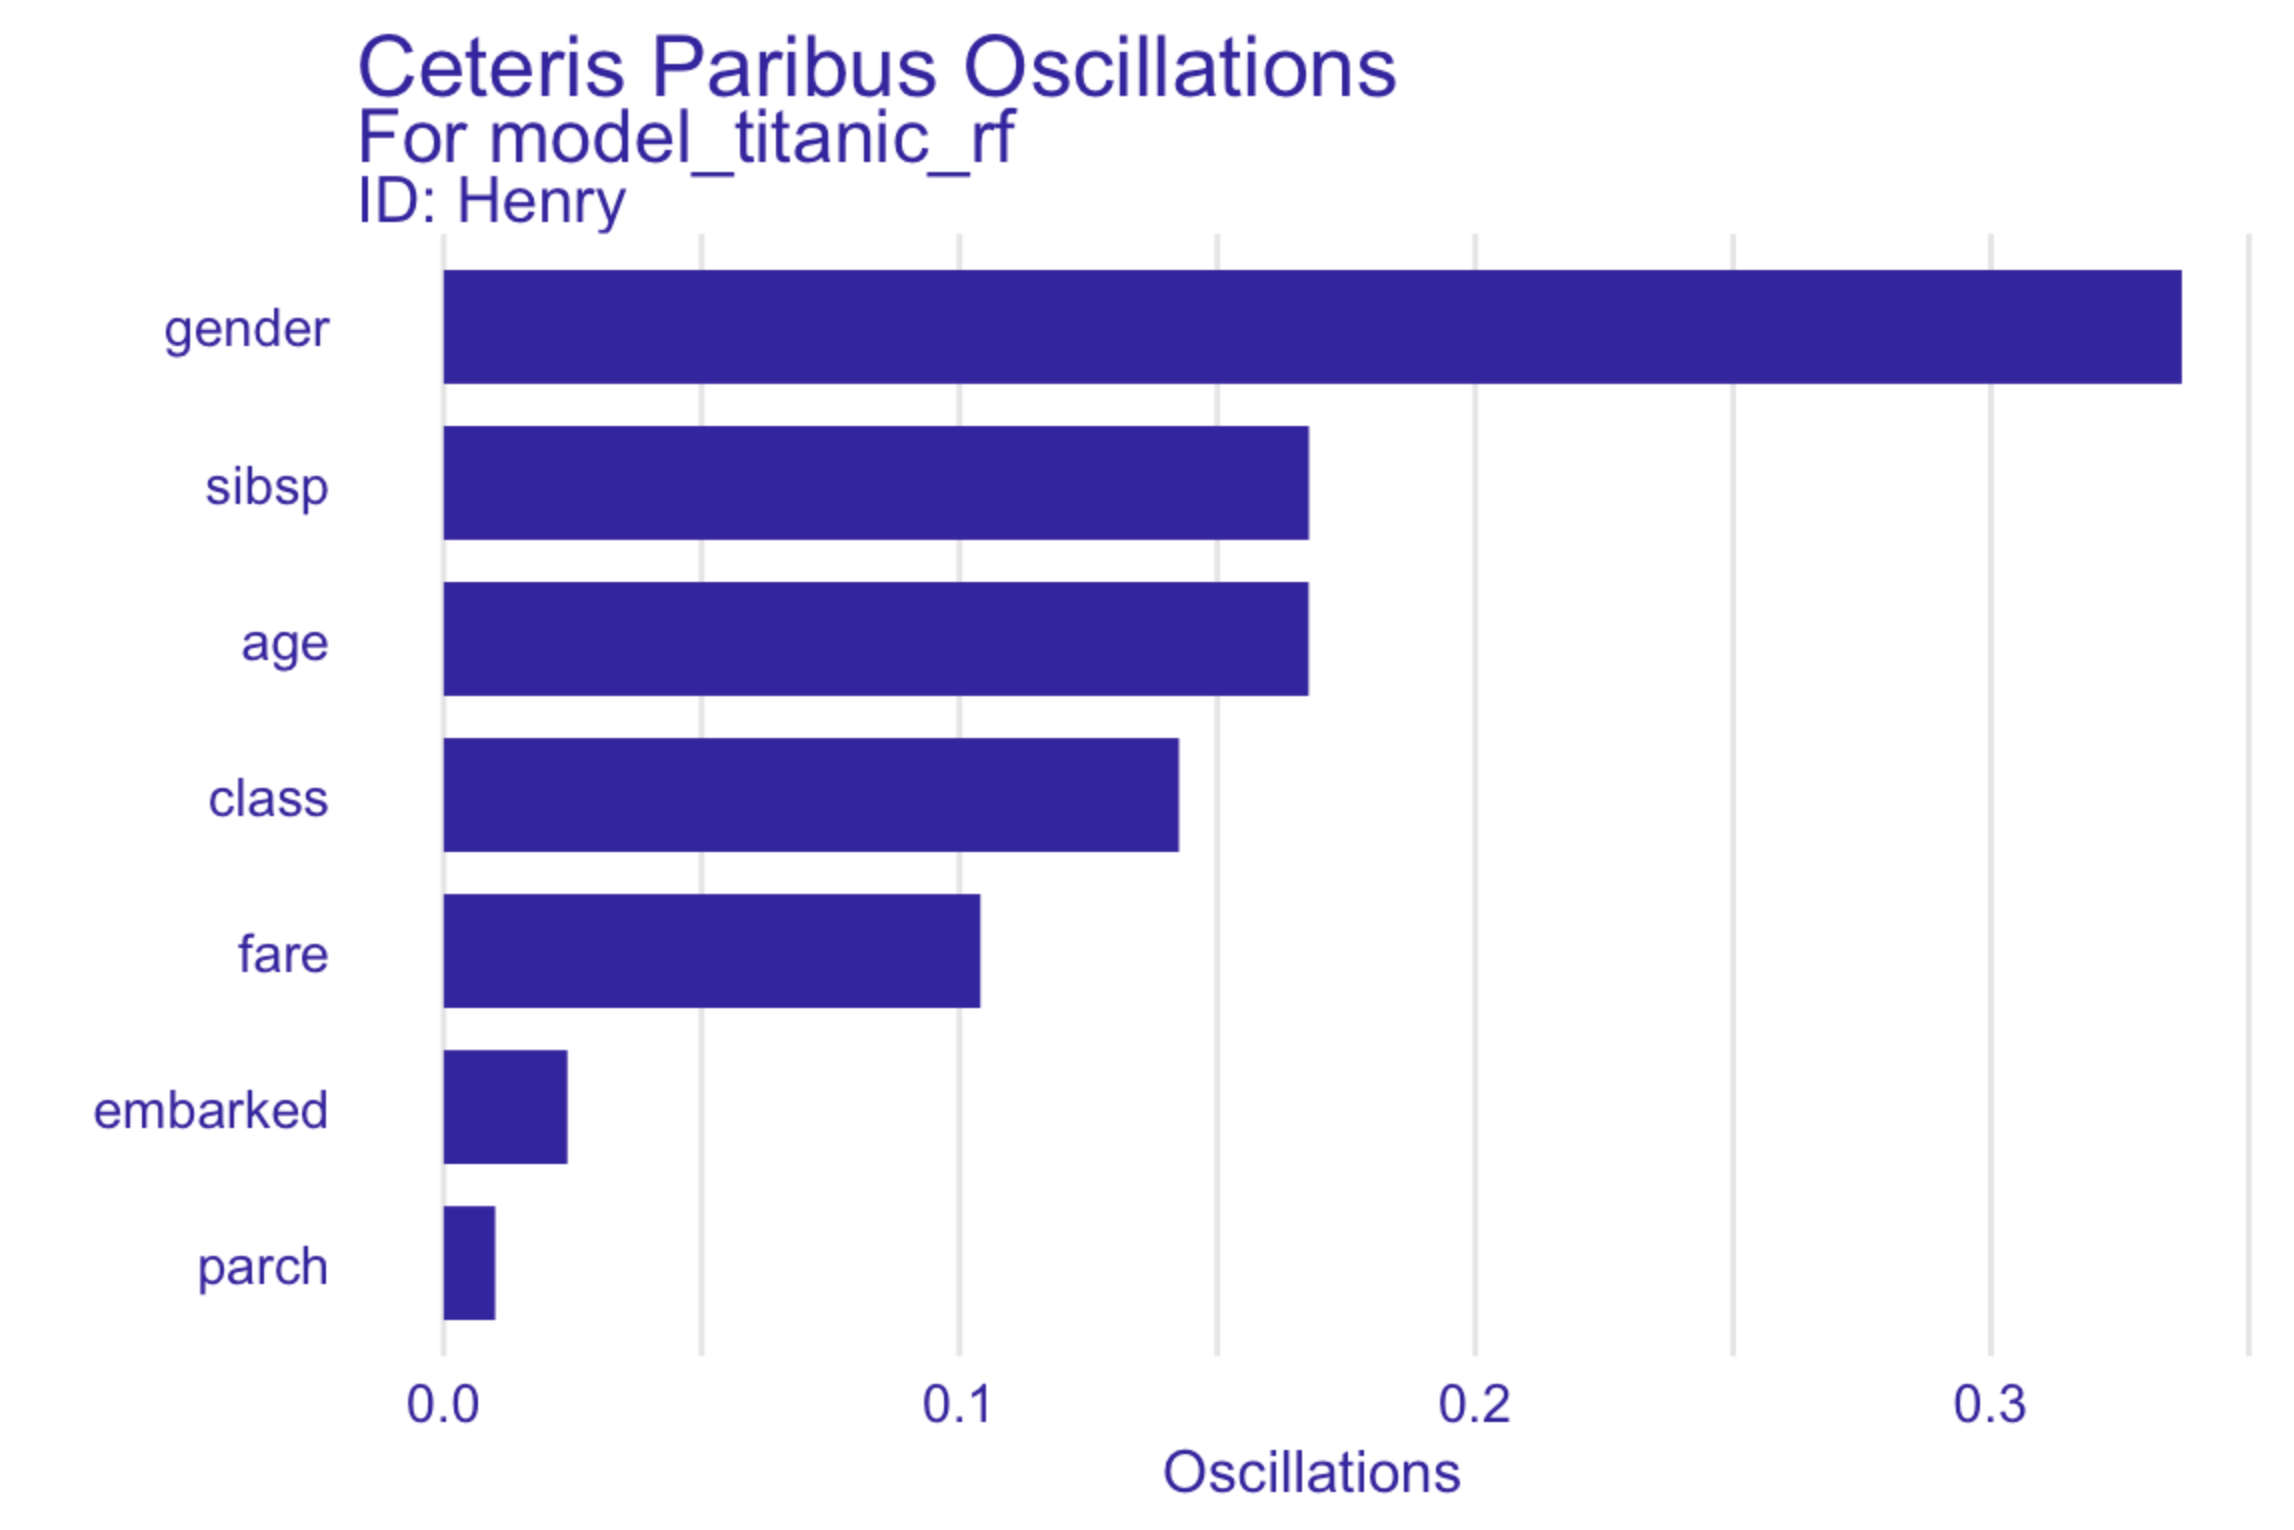
\includegraphics[width=0.75\linewidth]{figure/oscillations_all_rf_plot}

\}

\textbackslash{}caption\{(fig:CPVIP1) Variable-importance measures calculated for Ceteris-paribus oscillations for \texttt{henry} based on the \texttt{titanic\_rf\_v6} model\}\label{fig:CPVIP1}
\textbackslash{}end\{figure\}

\hypertarget{CPOscProsCons}{%
\subsection{Pros and cons}\label{CPOscProsCons}}

Oscillations of CP profiles are easy to interpret and understand. By using the average of oscillations, it is possible to select the most important variables for an instance prediction. This method can easily be extended to two or more variables. In such cases one needs to integrate the equation \eqref{eq:VIPCPuni} over larger number of variables.

There are several issues related to the use of the CP oscillations. For example, the oscillations may not be of help in situations when the use of CP profiles may itself be problematic (e.g., in the case of correlated explanatory variables or interactions - see Section \ref{CPProsCons}). An important issue is that the local variable importance do not sum up to the instance prediction for which they are calculated. In Chapters \ref{breakDown} and \ref{shapley}, we will introduce measures that address this problem.

\hypertarget{CPOscR}{%
\subsection{Code snippets for R}\label{CPOscR}}

In this section, we present key features of R package \texttt{ingredients} which is a part of the \texttt{DrWhy.AI} universe and covers all methods presented in this chapter. More details and examples can be found at \url{https://modeloriented.github.io/ingredients/}.

For illustration purposes we use the random forest model \texttt{titanic\_rf\_v6} (see Section \ref{odel-HR-rf}). Recall that it is developed to predict the probability of survival from sinking of Titanic. Instance-level explanations are calculated for a single observation: \texttt{henry} - a 47-year-old passenger that travelled in the 1st class.

\texttt{DALEX} explainers for both models and the Henry data are retrieved via \texttt{archivist} hooks as listed in Section \ref{ListOfModelsTitanic}.

\begin{Shaded}
\begin{Highlighting}[]
\KeywordTok{library}\NormalTok{(}\StringTok{"randomForest"}\NormalTok{)}
\NormalTok{explain_rf_v6 <-}\StringTok{ }\NormalTok{archivist}\OperatorTok{::}\KeywordTok{aread}\NormalTok{(}\StringTok{"pbiecek/models/9b971"}\NormalTok{)}

\KeywordTok{library}\NormalTok{(}\StringTok{"DALEX"}\NormalTok{)}
\NormalTok{henry <-}\StringTok{ }\NormalTok{archivist}\OperatorTok{::}\KeywordTok{aread}\NormalTok{(}\StringTok{"pbiecek/models/a6538"}\NormalTok{)}
\NormalTok{henry}
\end{Highlighting}
\end{Shaded}

\hypertarget{basic-use-of-the-calculate_oscillations-function}{%
\subsubsection{\texorpdfstring{Basic use of the \texttt{calculate\_oscillations} function}{Basic use of the calculate\_oscillations function}}\label{basic-use-of-the-calculate_oscillations-function}}

To calculate CP oscillations, we have got to calculate CP profiles for the selected observation. We use \texttt{henry} as the instance prediction of interest.

CP profiles are calculated by applying the \texttt{ceteris\_paribus()} function to the wrapper object.

\begin{Shaded}
\begin{Highlighting}[]
\KeywordTok{library}\NormalTok{(}\StringTok{"ingredients"}\NormalTok{)}
\KeywordTok{library}\NormalTok{(}\StringTok{"ggplot2"}\NormalTok{)}

\NormalTok{cp_titanic_rf <-}\StringTok{ }\KeywordTok{ceteris_paribus}\NormalTok{(explain_rf_v6, henry)}
\end{Highlighting}
\end{Shaded}

The resulting object can subsequently be processed with the \texttt{calculate\_oscillations()} function to calculate the oscillations and the estimated value of the variable-importance measure \eqref{eq:VIPCPdef}.

\begin{Shaded}
\begin{Highlighting}[]
\NormalTok{oscillations_titanic_rf <-}\StringTok{ }\KeywordTok{calculate_oscillations}\NormalTok{(cp_titanic_rf)}
\NormalTok{oscillations_titanic_rf}
\end{Highlighting}
\end{Shaded}

\begin{verbatim}
##    _vname_ _ids_ oscillations
## 2   gender     1   0.33700000
## 4    sibsp     1   0.15500000
## 3      age     1   0.14700000
## 1    class     1   0.14257143
## 6     fare     1   0.05407273
## 7 embarked     1   0.02400000
## 5    parch     1   0.00800000
\end{verbatim}

Note that, by default, \texttt{calculate\_oscillations()} estimates \(vip_{CP}^j(x_*)\) by \(\widehat{vip}_{CP}^{j,uni}(x_*)\), given in \eqref{eq:VIPCPuni}, using all unique values of the explanatory variable as the grid points.

The \texttt{calculate\_oscillations()} function returns an object of class \texttt{ceteris\_paribus\_oscillations}, which has a form of a data frame, but has also an overloaded \texttt{plot()} function. We can use the latter function to plot the local variable-importance measures for the instance of interest.

\begin{Shaded}
\begin{Highlighting}[]
\NormalTok{oscillations_titanic_rf}\OperatorTok{$}\StringTok{`}\DataTypeTok{_ids_}\StringTok{`}\NormalTok{ <-}\StringTok{ "Henry"}
\KeywordTok{plot}\NormalTok{(oscillations_titanic_rf) }\OperatorTok{+}\StringTok{ }\KeywordTok{ggtitle}\NormalTok{(}\StringTok{"Ceteris Paribus Oscillations"}\NormalTok{)}
\end{Highlighting}
\end{Shaded}

\begin{center}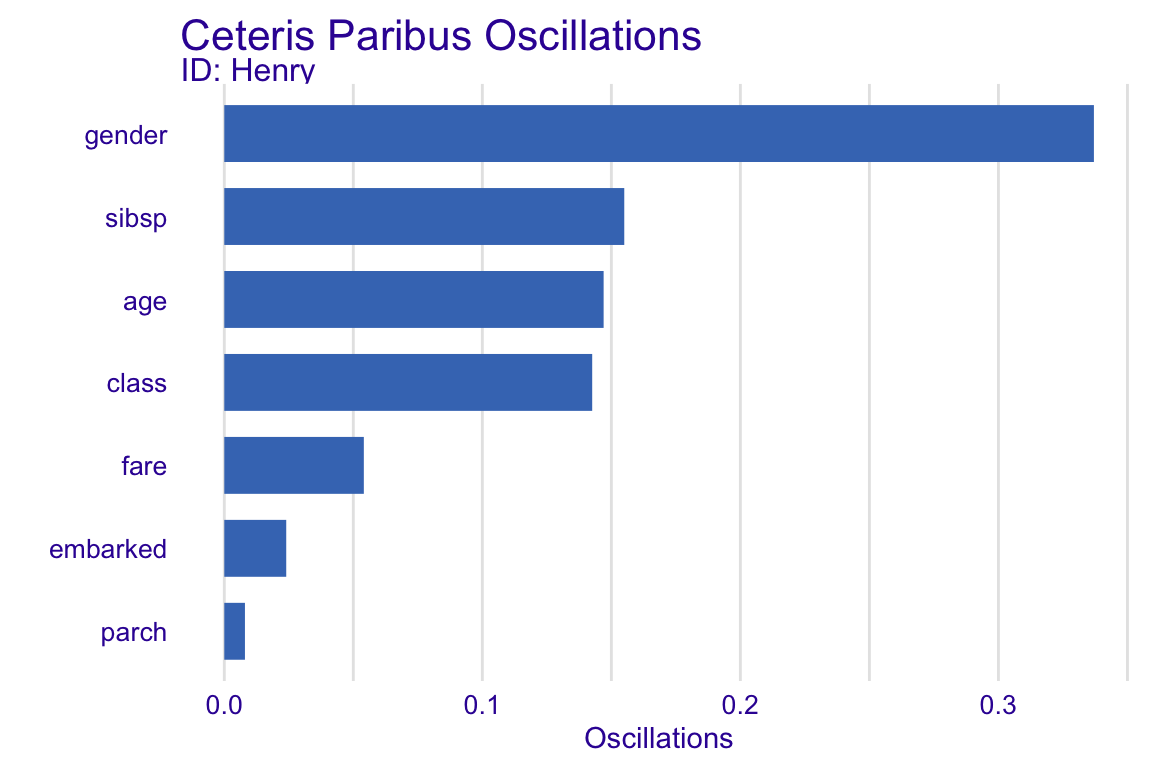
\includegraphics[width=0.7\linewidth]{PM_VEE_files/figure-latex/titanicCeterisProfile02E-1} \end{center}

\hypertarget{advanced-use-of-the-calculate_oscillations-function}{%
\subsubsection{\texorpdfstring{Advanced use of the \texttt{calculate\_oscillations} function}{Advanced use of the calculate\_oscillations function}}\label{advanced-use-of-the-calculate_oscillations-function}}

As mentioned in the previous section, \texttt{calculate\_oscillations()} estimates \(vip_{CP}^j(x_*)\) by \(\widehat{vip}_{CP}^{j,uni}(x_*)\) using all unique values of the explanatory variable as the grid points. However, other approaches are also possible.

One is to use \(\widehat{vip}_{CP}^{j,uni}(x_*)\), but assuming an equi-distant grid of values for a continuous explanatory variable. Toward this aim, we have got to explicitly specify a dense uniform grid of values for such a variable. The \texttt{variable\_splits} argument can be used for this purpose.

\begin{Shaded}
\begin{Highlighting}[]
\NormalTok{cp_titanic_rf_uniform <-}\StringTok{ }\KeywordTok{ceteris_paribus}\NormalTok{(explain_rf_v6, henry, }
              \DataTypeTok{variable_splits =} \KeywordTok{list}\NormalTok{(}\DataTypeTok{age =} \KeywordTok{seq}\NormalTok{(}\DecValTok{0}\NormalTok{, }\DecValTok{65}\NormalTok{, }\FloatTok{0.1}\NormalTok{),}
                                     \DataTypeTok{fare =} \KeywordTok{seq}\NormalTok{(}\DecValTok{0}\NormalTok{, }\DecValTok{200}\NormalTok{, }\FloatTok{0.1}\NormalTok{),}
                                     \DataTypeTok{sibsp =} \KeywordTok{seq}\NormalTok{(}\DecValTok{0}\NormalTok{, }\DecValTok{8}\NormalTok{, }\FloatTok{0.1}\NormalTok{),}
                                     \DataTypeTok{parch =} \KeywordTok{seq}\NormalTok{(}\DecValTok{0}\NormalTok{, }\DecValTok{8}\NormalTok{, }\FloatTok{0.1}\NormalTok{),}
                                     \DataTypeTok{gender =} \KeywordTok{unique}\NormalTok{(titanic}\OperatorTok{$}\NormalTok{gender),}
                                     \DataTypeTok{embarked =} \KeywordTok{unique}\NormalTok{(titanic}\OperatorTok{$}\NormalTok{embarked),}
                                     \DataTypeTok{class =} \KeywordTok{unique}\NormalTok{(titanic}\OperatorTok{$}\NormalTok{class)))}
\end{Highlighting}
\end{Shaded}

Subsequently, we apply the \texttt{calculate\_oscillations()} function to compute the oscillations and the variable-importance measures.

\begin{Shaded}
\begin{Highlighting}[]
\NormalTok{oscillations_uniform <-}\StringTok{ }\KeywordTok{calculate_oscillations}\NormalTok{(cp_titanic_rf_uniform)}
\NormalTok{oscillations_uniform}\OperatorTok{$}\StringTok{`}\DataTypeTok{_ids_}\StringTok{`}\NormalTok{ <-}\StringTok{ "Henry"}
\NormalTok{oscillations_uniform}
\end{Highlighting}
\end{Shaded}

\begin{verbatim}
##    _vname_ _ids_ oscillations
## 5   gender Henry    0.3370000
## 3    sibsp Henry    0.1677778
## 1      age Henry    0.1677235
## 7    class Henry    0.1425714
## 2     fare Henry    0.1040790
## 6 embarked Henry    0.0240000
## 4    parch Henry    0.0100000
\end{verbatim}

\begin{Shaded}
\begin{Highlighting}[]
\KeywordTok{plot}\NormalTok{(oscillations_uniform) }\OperatorTok{+}\StringTok{ }\KeywordTok{ggtitle}\NormalTok{(}\StringTok{"Ceteris Paribus Oscillations"}\NormalTok{, }\StringTok{"Expectation over uniform distribution"}\NormalTok{)}
\end{Highlighting}
\end{Shaded}

\begin{center}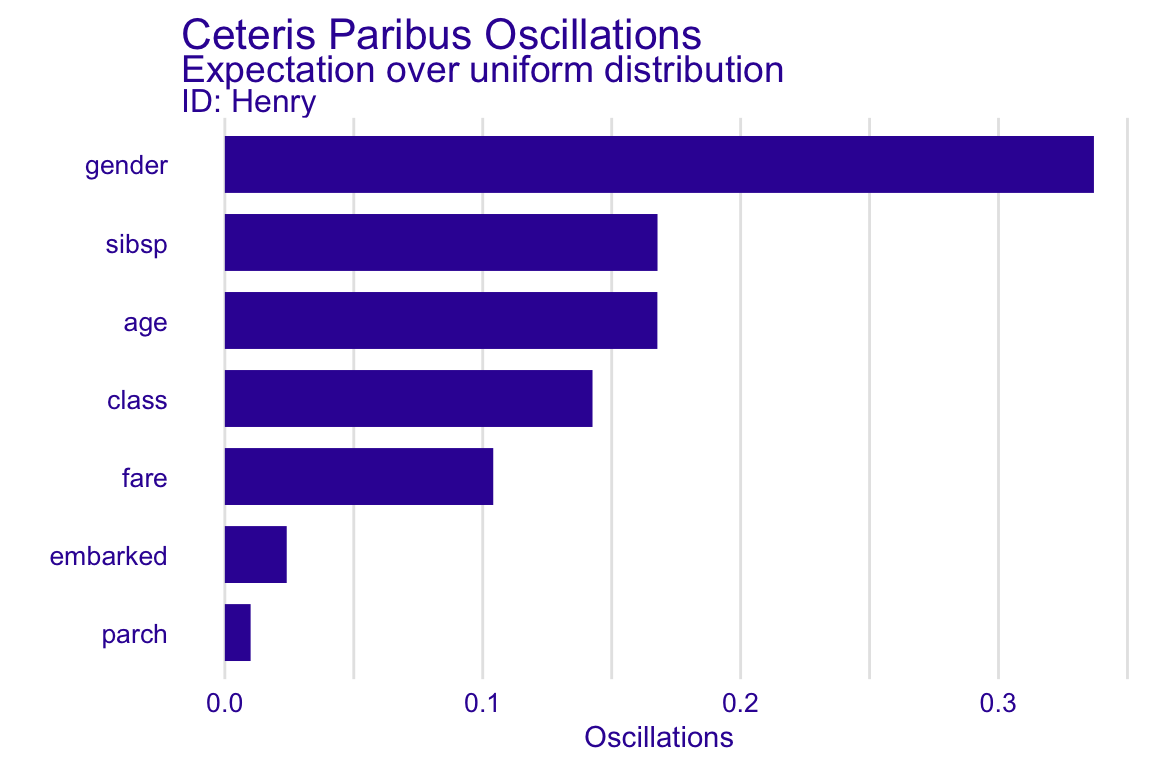
\includegraphics[width=0.7\linewidth]{PM_VEE_files/figure-latex/titanicCeterisProfile02G-1} \end{center}

Another approach is to calculate the expectation \eqref{eq:VIPCPdef} over the empirical distribution of a variable, i..e, to use \(\widehat{vip}_{CP}^{j,emp}(x_*)\), given in \eqref{eq:VIPCPemp}. Toward this aim, we use the \texttt{variable\_splits} argument to explicitly specify the validation-data sample to define the grid of values.

\begin{Shaded}
\begin{Highlighting}[]
\NormalTok{titanic <-}\StringTok{ }\KeywordTok{na.omit}\NormalTok{(titanic)}

\NormalTok{cp_titanic_rf_empirical <-}\StringTok{ }\KeywordTok{ceteris_paribus}\NormalTok{(explain_rf_v6, henry, }
              \DataTypeTok{variable_splits =} \KeywordTok{list}\NormalTok{(}\DataTypeTok{age =}\NormalTok{ titanic}\OperatorTok{$}\NormalTok{age,}
                                     \DataTypeTok{fare =}\NormalTok{ titanic}\OperatorTok{$}\NormalTok{fare,}
                                     \DataTypeTok{sibsp =}\NormalTok{ titanic}\OperatorTok{$}\NormalTok{sibsp,}
                                     \DataTypeTok{parch =}\NormalTok{ titanic}\OperatorTok{$}\NormalTok{parch,}
                                     \DataTypeTok{gender =}\NormalTok{ titanic}\OperatorTok{$}\NormalTok{gender,}
                                     \DataTypeTok{embarked =}\NormalTok{ titanic}\OperatorTok{$}\NormalTok{embarked,}
                                     \DataTypeTok{class =}\NormalTok{ titanic}\OperatorTok{$}\NormalTok{class))}
\end{Highlighting}
\end{Shaded}

\begin{Shaded}
\begin{Highlighting}[]
\NormalTok{oscillations_empirical <-}\StringTok{ }\KeywordTok{calculate_oscillations}\NormalTok{(cp_titanic_rf_empirical)}
\NormalTok{oscillations_empirical}\OperatorTok{$}\StringTok{`}\DataTypeTok{_ids_}\StringTok{`}\NormalTok{ <-}\StringTok{ "Henry"}
\NormalTok{oscillations_empirical}
\end{Highlighting}
\end{Shaded}

\begin{verbatim}
##    _vname_ _ids_ oscillations
## 1      age Henry  0.153323969
## 5   gender Henry  0.149336656
## 7    class Henry  0.133567739
## 2     fare Henry  0.056883552
## 3    sibsp Henry  0.035932034
## 6 embarked Henry  0.019818758
## 4    parch Henry  0.001623924
\end{verbatim}

\begin{Shaded}
\begin{Highlighting}[]
\KeywordTok{plot}\NormalTok{(oscillations_empirical) }\OperatorTok{+}\StringTok{ }\KeywordTok{ggtitle}\NormalTok{(}\StringTok{"Ceteris Paribus Oscillations"}\NormalTok{, }\StringTok{"Expectation over empirical distribution"}\NormalTok{)}
\end{Highlighting}
\end{Shaded}

\begin{center}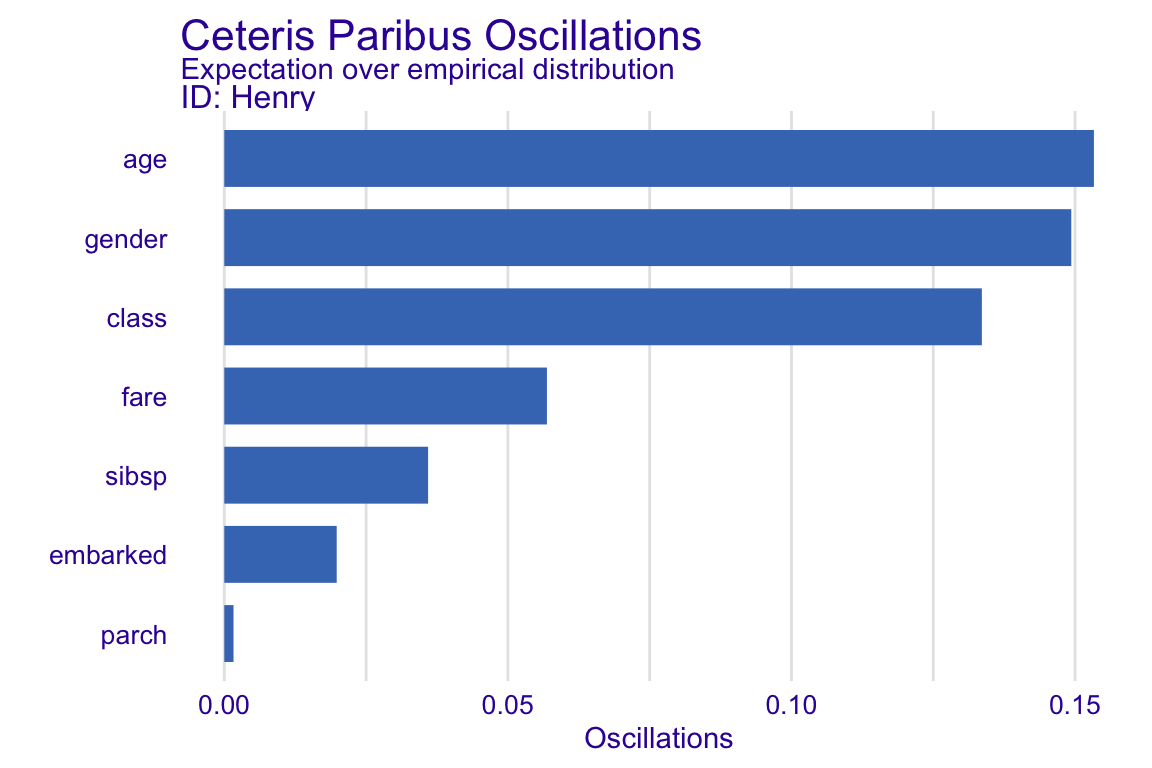
\includegraphics[width=0.7\linewidth]{PM_VEE_files/figure-latex/titanicCeterisProfile02I-1} \end{center}

\hypertarget{localDiagnostics}{%
\section{Local Diagnostics With Ceteris-paribus Profiles}\label{localDiagnostics}}

\hypertarget{cPLocDiagIntro}{%
\subsection{Introduction}\label{cPLocDiagIntro}}

It may happen that, while the global predictive performance of the model is good, model predictions for some observations are very bad. In this chapter, we present two local-diagnostics techniques that can address this issue. In particular, we focus on fidelity plots: the plot of CP profiles for nearest neighbors and the local-fidelity plot.

The idea behind fidelity plots is to select a number of observations (``neighbors'') from the validation dataset that are closest to the instance (observation) of interest. Then, for the selected observations, we plot CP profiles and check how stable they are. Additionally, if we know true values of the dependent variable for the selected neighbors, we may add residuals to the plot to evaluate the local fit of the model.

\hypertarget{cPLocDiagIntuition}{%
\subsection{Intuition}\label{cPLocDiagIntuition}}

One approach to local model diagnostics is to examine how the predictions vary for observations from the training dataset. Figure \ref{fig:profileWith10NN} presents CP profiles for the instance of interest and its 10 nearest neighbors for the random forest model for the Titanic dataset (Section \ref{model-titanic-rf}). The profiles are almost parallel and very close to each other. This suggests that model predictions are stable around the instance of interest, because small changes in the explanatory variables (represented by the nearest neighbors) have not got much influence on the predictions.

\textbackslash{}begin\{figure\}

\{\centering 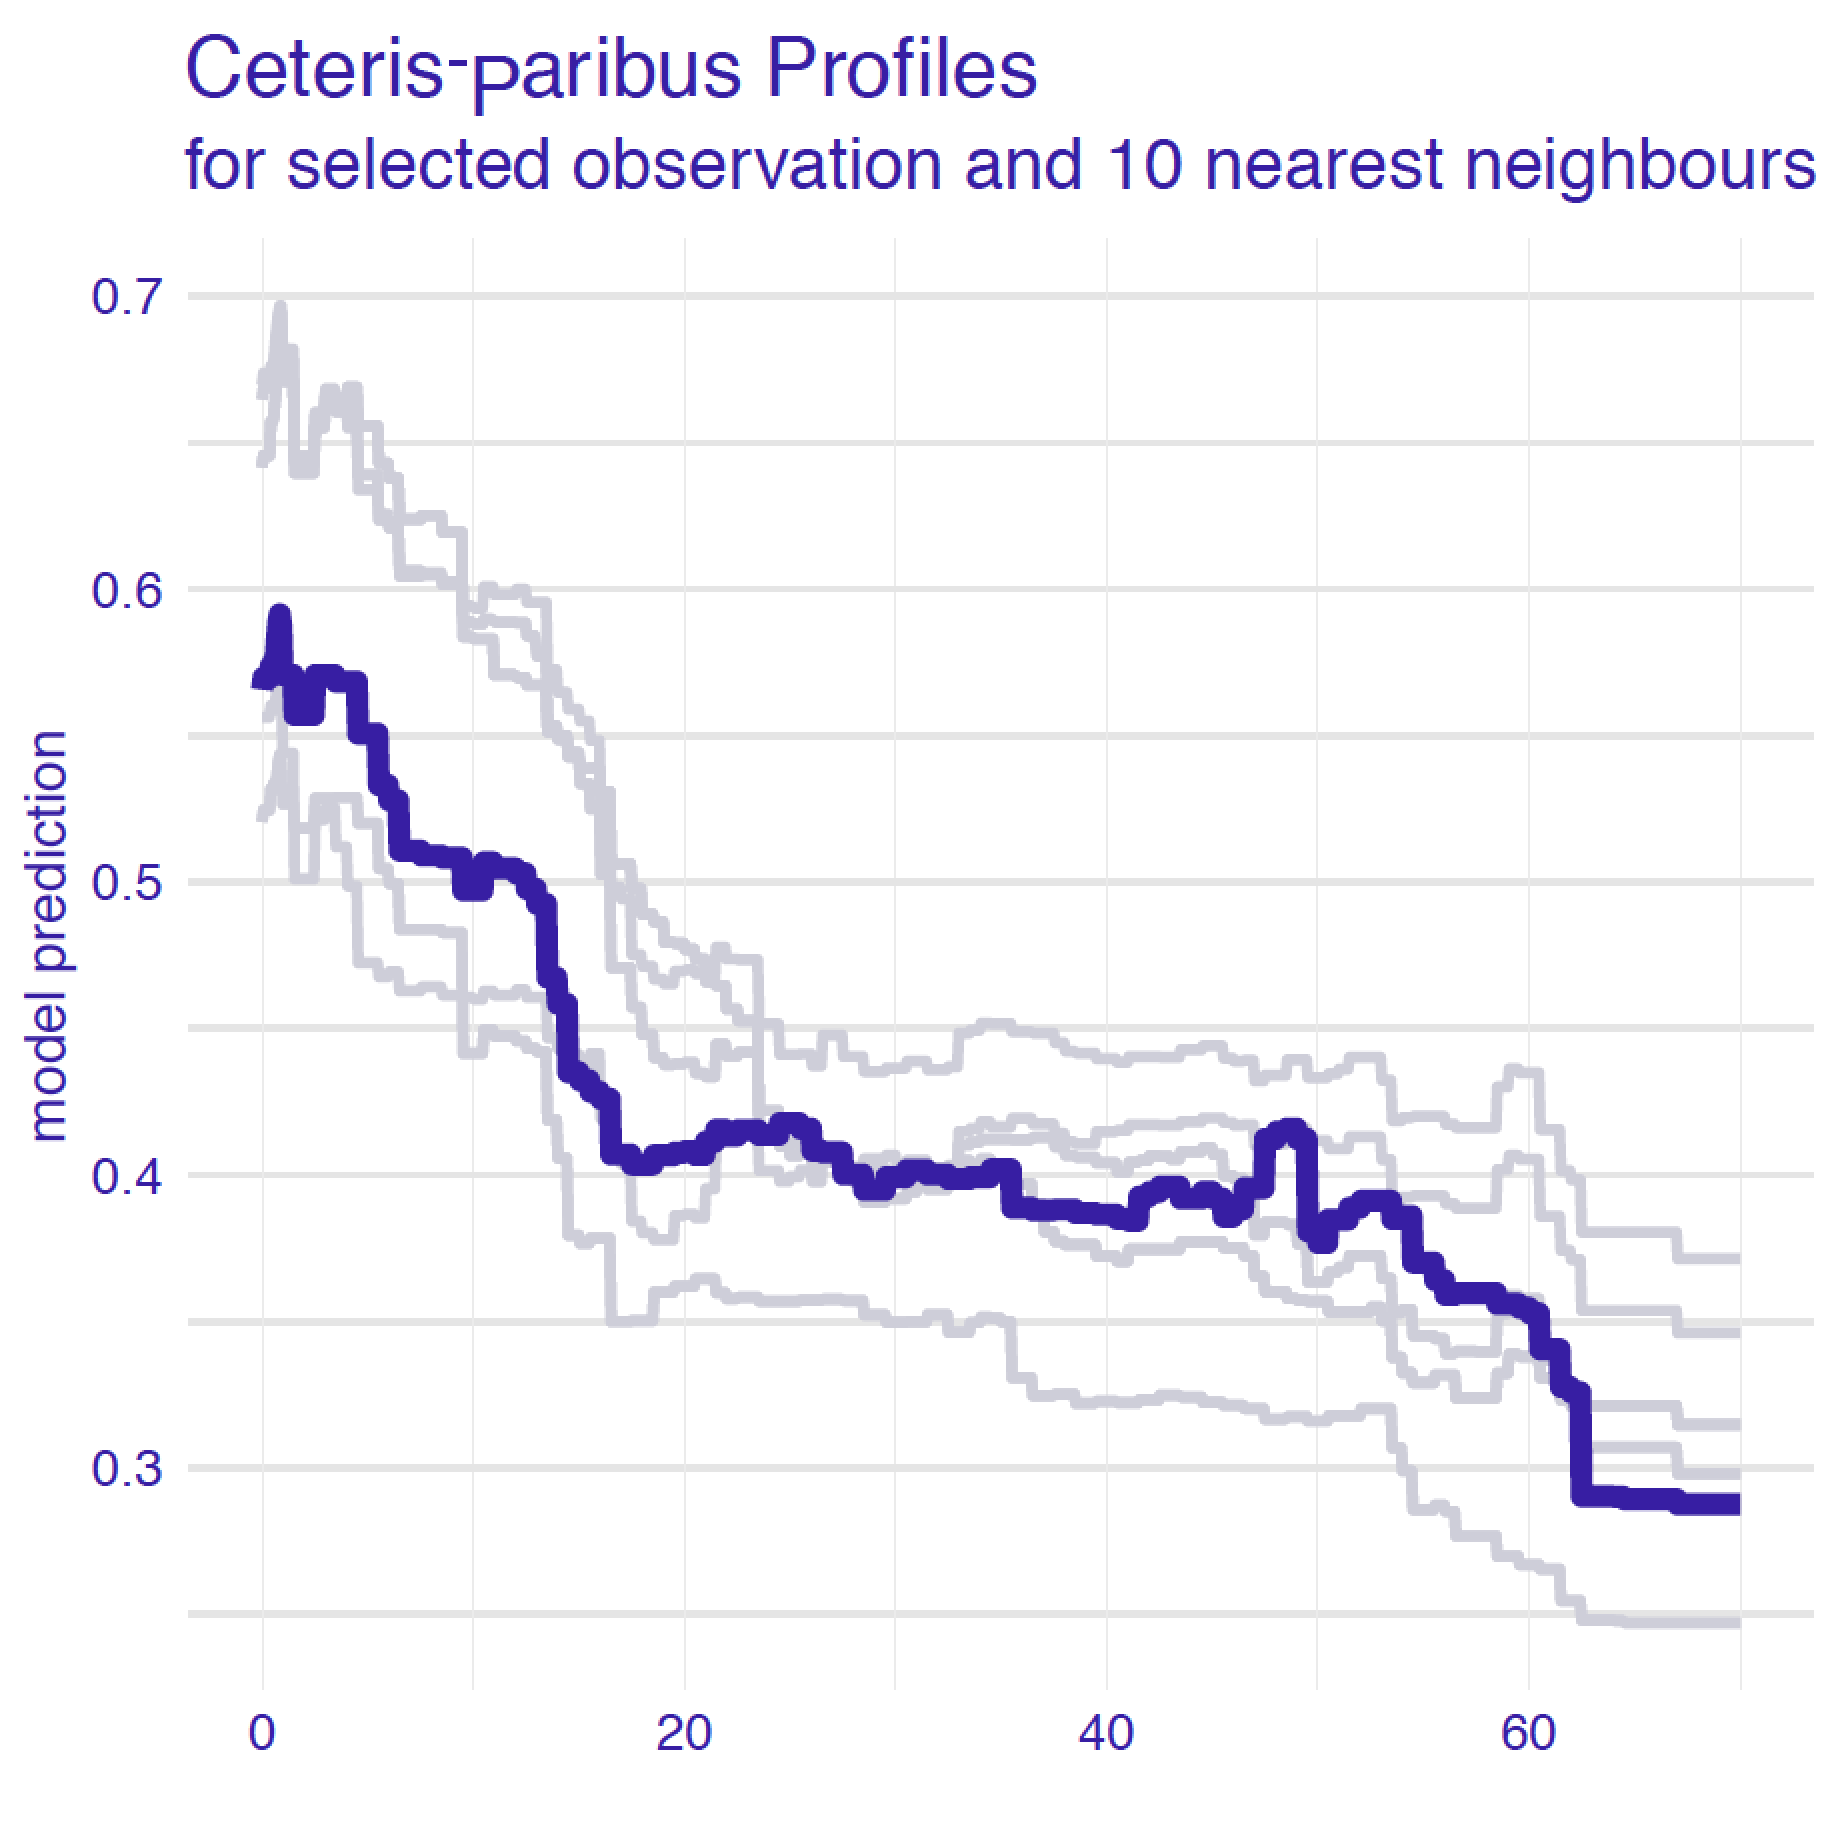
\includegraphics[width=0.5\linewidth]{figure/example_cp}

\}

\textbackslash{}caption\{(fig:profileWith10NN) Ceteris-paribus profiles for a selected instance (dark violet line) and 10 nearest neighbors (light grey lines) for the \texttt{titanic\_rf\_b6} model. The profiles are almost parallel and close to each other what suggests the stability of the model.\}\label{fig:profileWith10NN}
\textbackslash{}end\{figure\}

Once we have selected the nearest neighbors, we can also look closer at the model fit around the point of interest.
Figure \ref{fig:profileBack2BackHist} presents histograms of residuals for the entire dataset and the selected neighbors for the random forest model for the Apartments dataset (Section \ref{model-Apartments-rf}). The distribution of residuals for the entire dataset is rather symmetric and centered around 0, suggesting a reasonable average performance of the model. On the other hand, the residuals for the selected neighbors are centered around the value of 500. This sugests that, on average, the model predictions are biased for the instance of interest.

\textbackslash{}begin\{figure\}

\{\centering 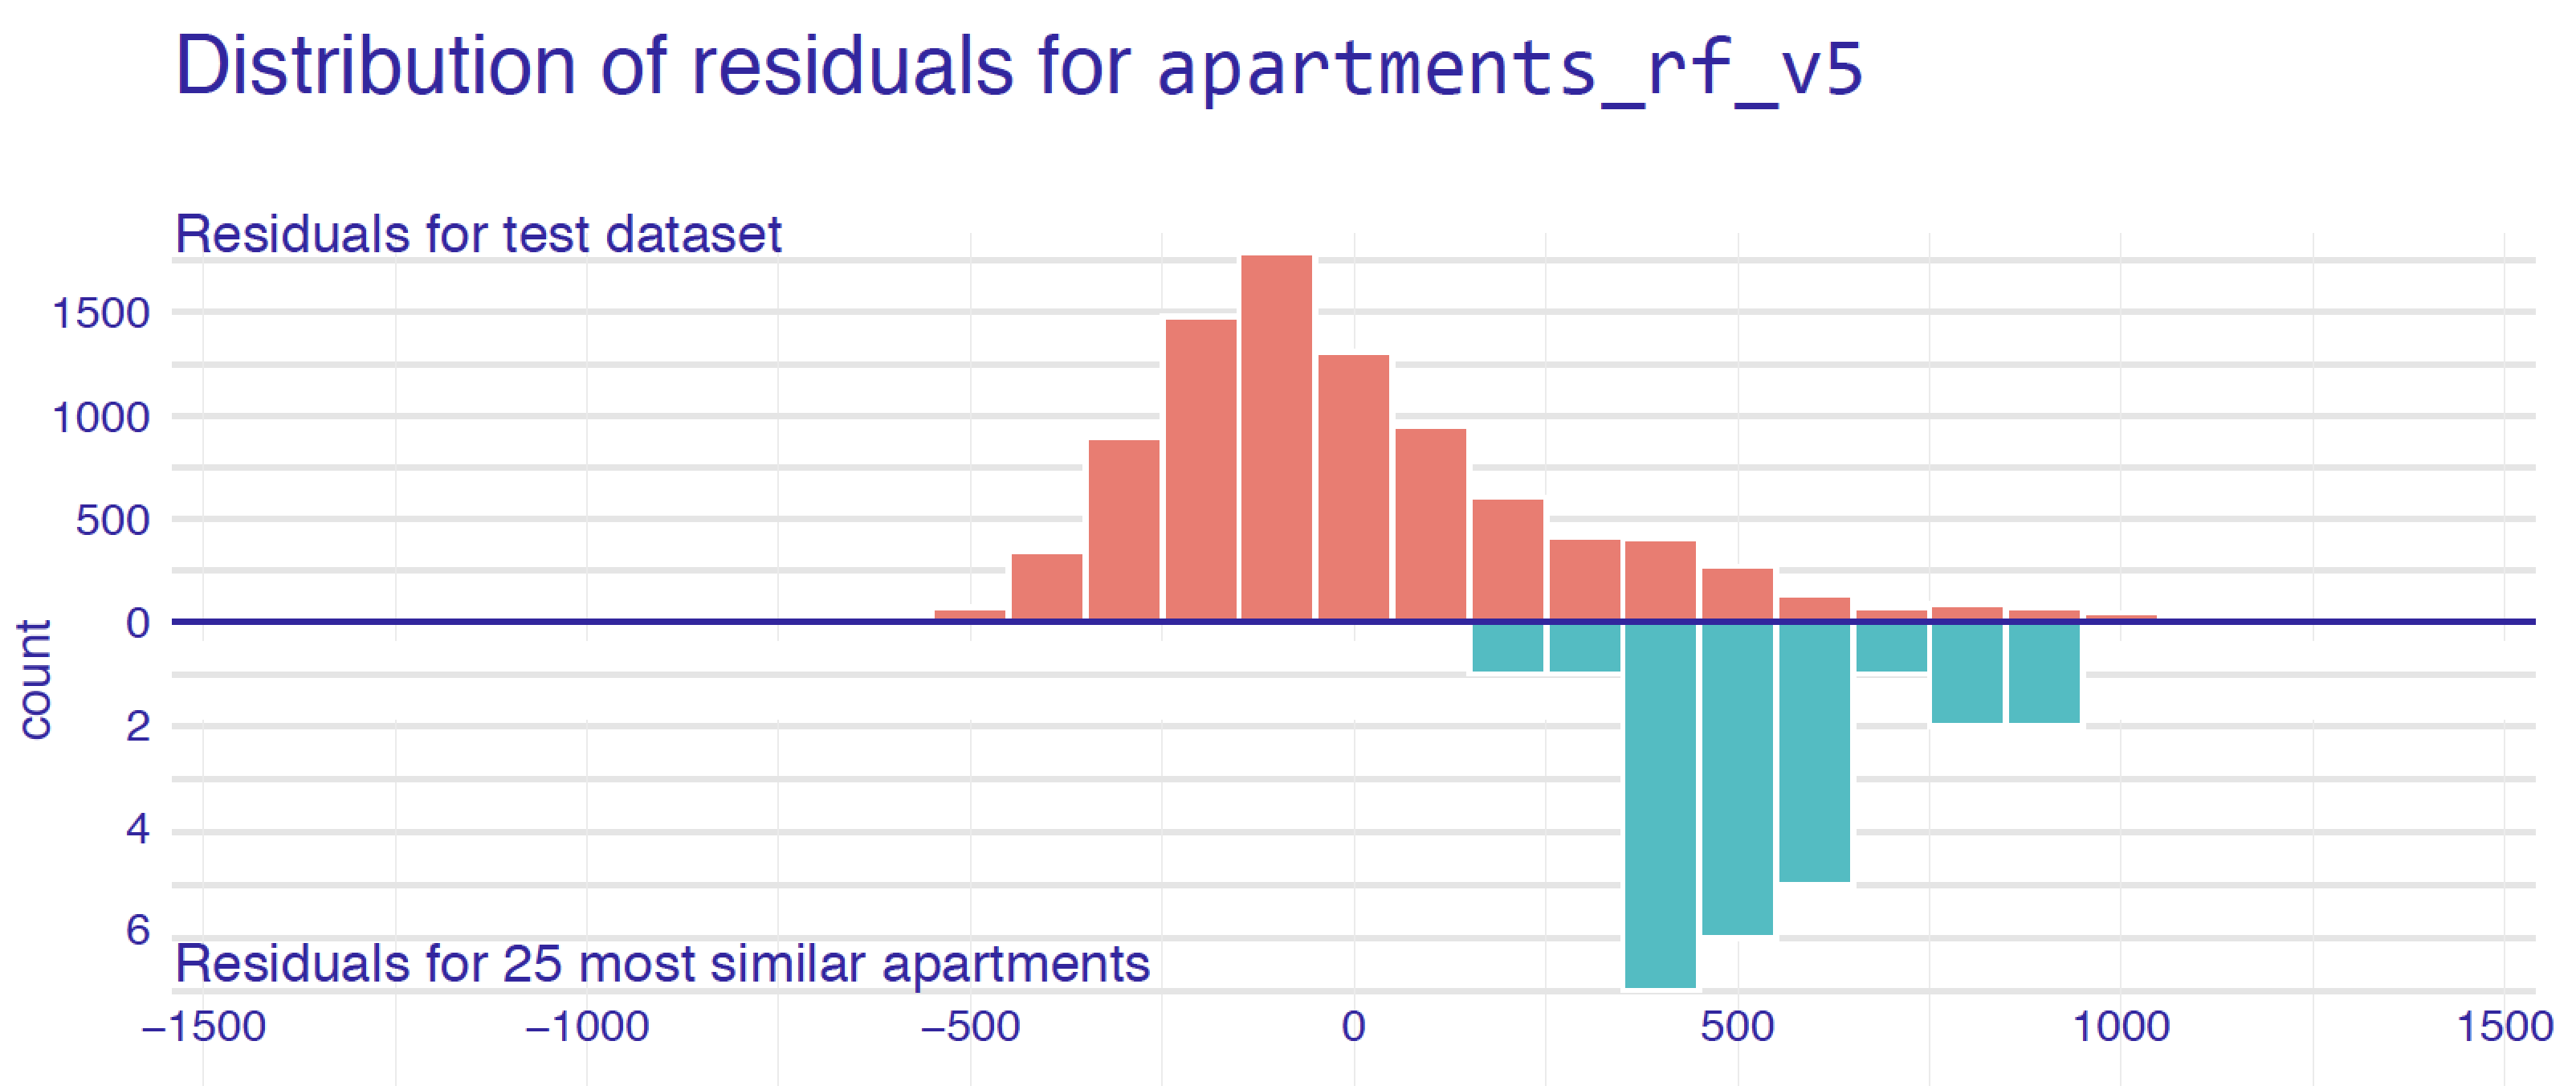
\includegraphics[width=0.7\linewidth]{figure/bb_hist}

\}

\textbackslash{}caption\{(fig:profileBack2BackHist) Histograms of residuals for the \texttt{apartments\_rf\_v5} model for the Apartments dataset. Upper panel: residuals calculated for all observations from the dataset. Bottom panel: residuals calculated for 25 nearest neighbors of the instance of interest.\}\label{fig:profileBack2BackHist}
\textbackslash{}end\{figure\}

\hypertarget{cPLocDiagMethod}{%
\subsection{Method}\label{cPLocDiagMethod}}

The proposed method is based on three elements:

\begin{itemize}
\tightlist
\item
  identification of nearest neighbors,
\item
  calculation and visualization of CP profiles for the selected neighbors, and
\item
  analysis of residuals for the neighbors.
\end{itemize}

In what follows we discuss each of the elements in more detail.

\hypertarget{cPLocDiagNeighbors}{%
\subsubsection{Nearest neighbors}\label{cPLocDiagNeighbors}}

There are two important questions related to the selection of the neighbors ``nearest'' to the instance (observation) of interest:

\begin{itemize}
\tightlist
\item
  How many neighbors should we choose?
\item
  What metric should be used to measure the ``proximity'' of observations?
\end{itemize}

The answer to both questions is, of course, \emph{it depends}.

\begin{itemize}
\tightlist
\item
  The smaller the number of neighbors, the more local is the analysis. However, a very small number will lead to a larger variability of the results. In many cases we found that 20 neighbors works fine. However, one should always take into account computational time (smaller number of neighbors results in quicker calculations) and the size of the dataset (for a small dataset, smaller sets of neighbors may be preferred).
\item
  The metric is very important. The more explanatory variables, the more important is the choice. In particular, the metric should be capable of accommodating variables of different nature (categorical, continuous). Our default choice is the Gower similarity measure:
\end{itemize}

\[
d_{gower}(x_i, x_j) = \frac 1p \sum_{k=1}^p d^k(x_i^k, x_j^k),
\]
where \(x_i\) is a \(p\)-dimensional vector of explanatory covariates for the \(i\)-th observation and \(d^k(x_i^k,x_j^k)\) is the distance between values of the \(k\)-th variable for the \(i\)-th and \(j\)-th observations. Note that \(d^k()\) depends on the nature of the variable. For instance, for a continuous variable it is equal to \(|x_i^k-x_j^k|/\{max(x_1^k,\ldots,x_n^k)-min(x_1^k,\ldots,x_n^k)\}\), i.e., the absolute difference scaled by the observed range of the variable. On the other hand, for a categorical variable, it is simply \(I(x_i^k = x_j^k)\), where \(I()\) is the indicator function. Note that \(p\) may be equal to the number of all explanatory variables included in the model, or only a subset of them. An advantage of Gower similarity measure is that it ``deals'' with heterogeneous vectors with both categorical and continuous variables.

Once we have decided on the number of neighbors, we can use the chosen metric to select the required number observations ``closest'' to the one of interest.

\hypertarget{cPLocDiagProfiles}{%
\subsubsection{Profiles for neighbors}\label{cPLocDiagProfiles}}

Once nearest neighbors have been identified, we can graphically compare CP profiles for selected (or all) variables.

For a model with a large number of variables, we may end up with a large number of plots. In such a case a better strategy is to focus only on \(K\) most important variables, selected by using the variable-importance measure (see Chapter \ref{ceterisParibusOscillations}).

\hypertarget{cPLocDiagLFplot}{%
\subsubsection{Local-fidelity plot}\label{cPLocDiagLFplot}}

CP profiles are helpful to assess the model stability. In addition, we can enhance the plot by adding residuals to it to allow evaluation of the local model fit. For model \(f()\) and observation \(i\) described by the vector of explanatory variables \(x_i\), the residual is the difference between the observed and predicted value of the dependent variable \(Y_i\), i.e.,

\[
r_i = y_i - f(x_i).
\]
Note that, for a binary variable, the residual is the difference between the value of 0 or 1, depending on how we code ``success,'' and the value of the predicted probability of ``success.'' This defintion also applies to categorical responses, as it is common to define, in such case, a binary ``success'' indicator and compute the predicted probaiblity of ``success'' for each category separately.

The plot that includes CP profiles for the nearest neighbors and the corresponding residuals is called a local-fidelity plot.

\hypertarget{cPLocDiagExample}{%
\subsection{Example: Titanic}\label{cPLocDiagExample}}

As an example, we will use the predictions for the random forest model for the Titanic data (see Section \ref{model-titanic-rf}).

Figure \ref{fig:localFidelityPlots} presents a detailed explanation of the elements of a local-fidelity plot for \emph{age}, a continuous explanatory variable. The plot includes eight nearest neighbors of Henry (see Section \ref{predictions-titanic}). Profiles are quite apart from each other, which indicates potential instability of model predictions. However, the residuals included in the plots are positive and negative, indicating that, on average, the instance prediction should not be biased.

Figure \ref{fig:localFidelityPlots2} presents a local-fidelity plot for the categorical explanatory variable \texttt{class}. Henry and his neighbors traveled in the \texttt{1st} class. In different panels we see how the predicted probabilityof survival changes if the \texttt{1st} class is replaced, for instance, by the \texttt{2nd} (in most cases, they probability will be reduced) or the \texttt{deck\ crew} (in most cases, the probability will increase). Such plots can help to detect interactions, as we see that the same change (let's say, from the \texttt{1st} to the \texttt{3rd} class) results in a different change of the model prediction.

\begin{figure}

{\centering 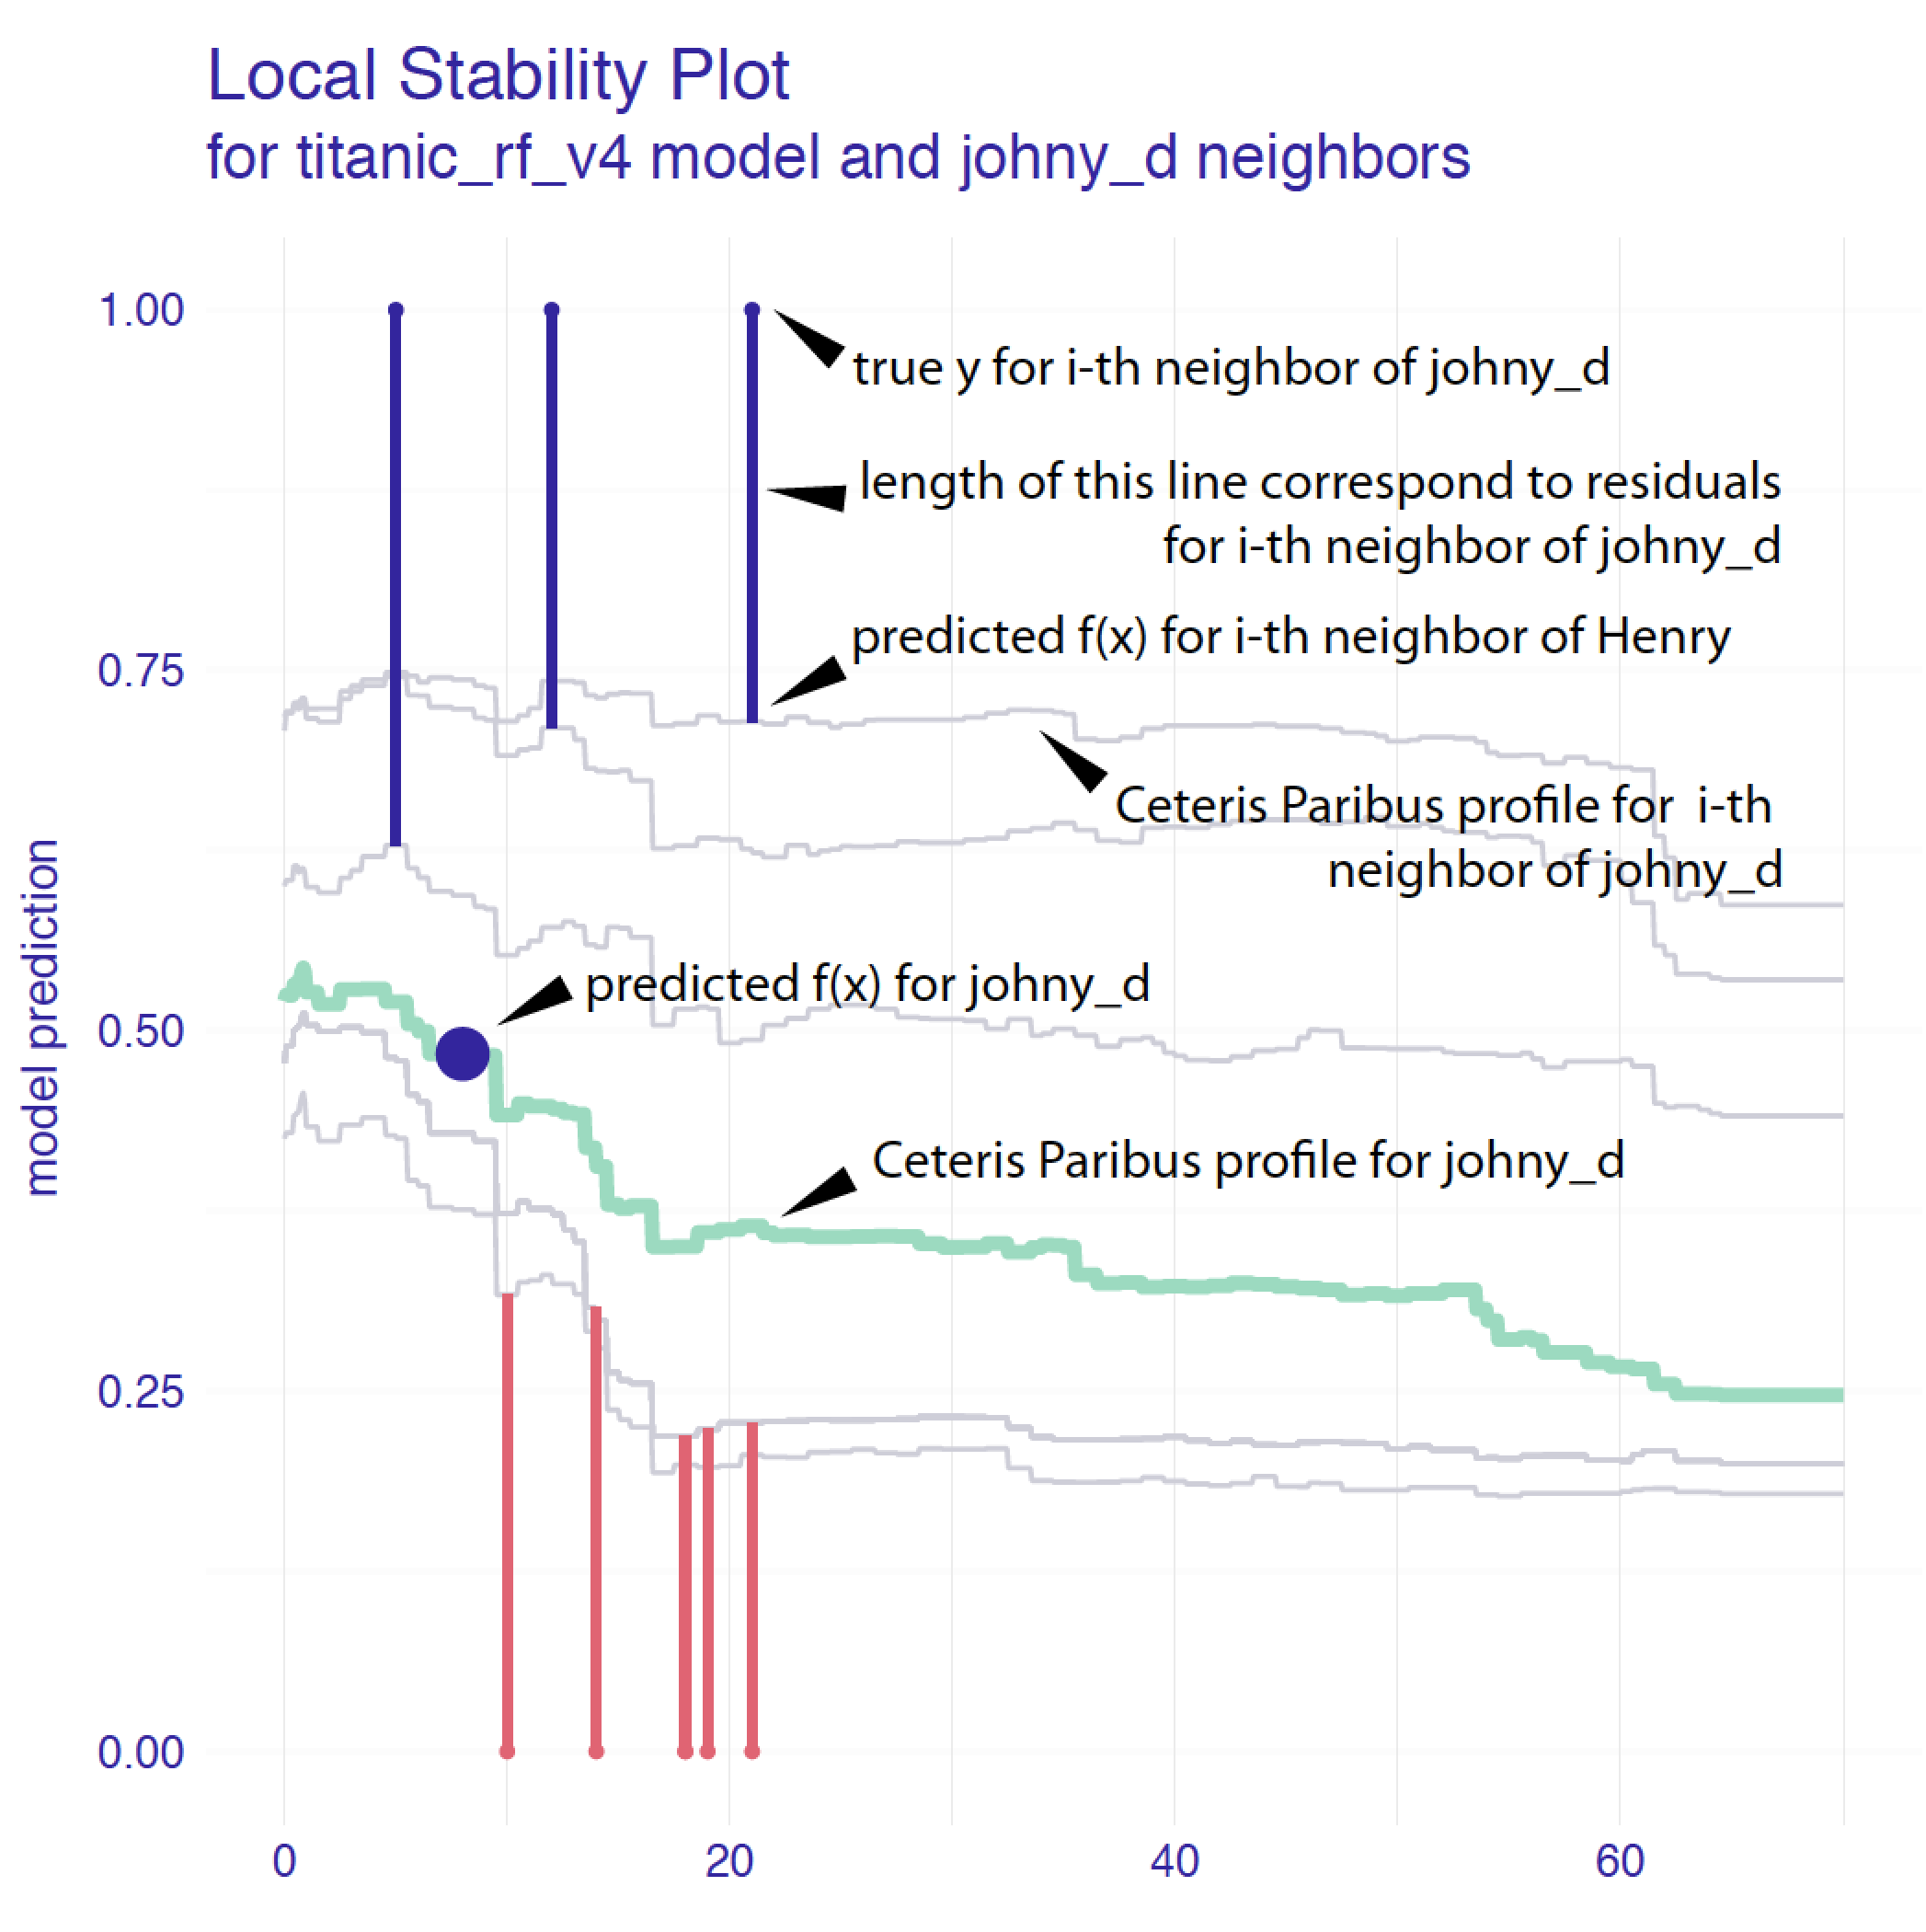
\includegraphics[width=0.7\linewidth]{figure/localFidelityPlots} 

}

\caption{(fig:localFidelityPlots) Elements of a local-fidelity plot for a continuous explanatory variable. The green line shows the Ceteris-paribus profile for the instance of interest. Profiles of the nearest neighbors are marked with grey lines. The vertical intervals correspond to residuals; the shorter the interval, the smaller the residual and the more accurate prediction of the model. Blue intervals correspond to positive residuals, red intervals to negative intervals. Stable model will have profiles close to each other; additive model will have parallel lines.}\label{fig:localFidelityPlots}
\end{figure}

\begin{figure}

{\centering 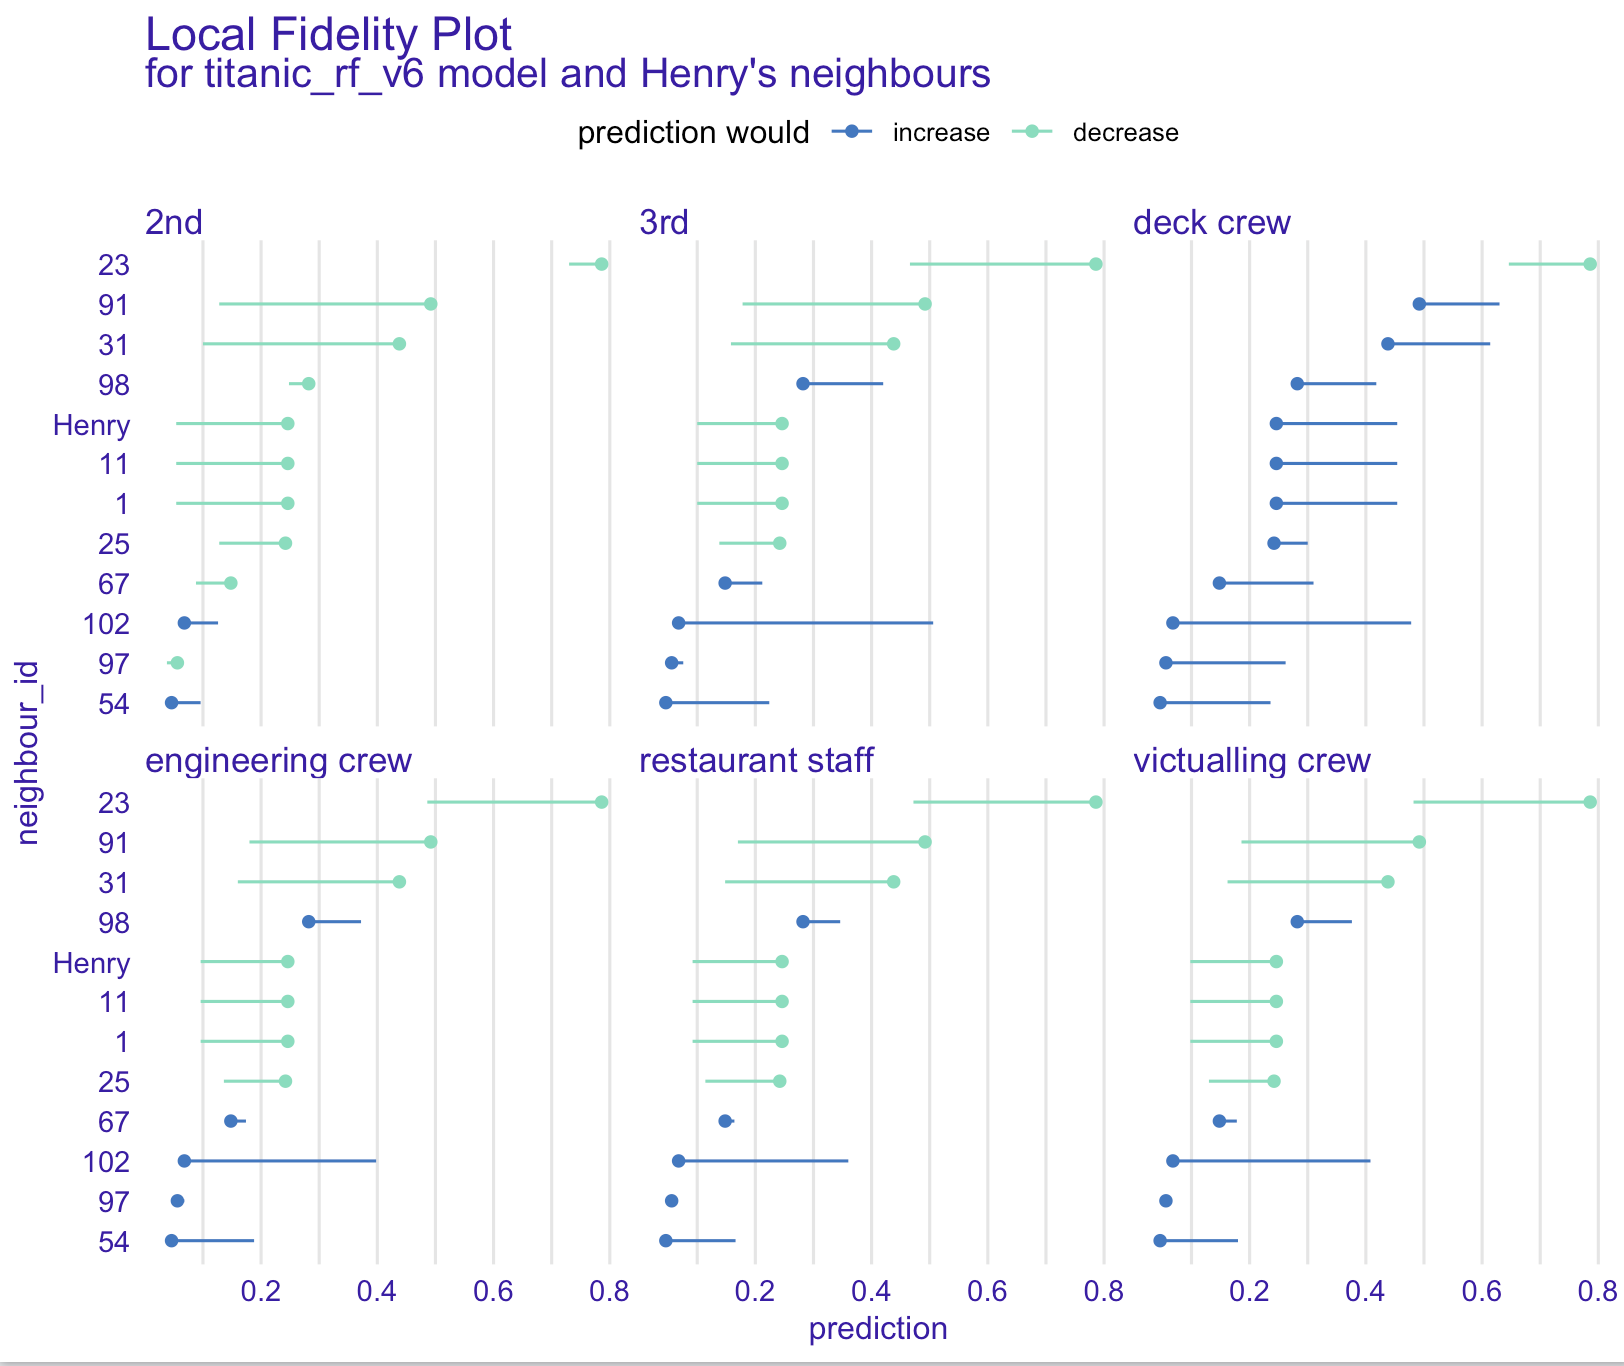
\includegraphics[width=0.7\linewidth]{figure/cp_fidelity_2} 

}

\caption{(fig:localFidelityPlots2) The local-fidelity plot for the categorical explanatory variable `class` in the random effects model for the Titanic data, Henry, and his 10 neighbors. Each panel indicates how the model prediction would change if the class changed from  `1st` to another one. Dots indicate original model predictions for the neighbors; the end of the interval corresponds to model prediction after changing the class. The top-lef panel indicates that, for the majority of the neighbors, the change from the `1st` to the `2nd` class reduces the predicted value of the probability of survival. On the other hand, the top-right panel indicates that changing the lass to `deck crew` members increases the predicted probability.}\label{fig:localFidelityPlots2}
\end{figure}

\hypertarget{cPLocDiagProsCons}{%
\subsection{Pros and cons}\label{cPLocDiagProsCons}}

Local-fidelity plots may be very helpful to check if

\begin{itemize}
\tightlist
\item
  the model is locally additive, as for such models the CP profiles should be parallel;
\item
  the model is locally stable, as in that case the CP profiles should be close to each other;
\item
  the model fit for the instance of interest is good, as in that case the residuals should be small and their distribution should be balanced around 0.
\end{itemize}

The drawback is that such plots are quite complex and lack objective measures of the quality of the model fit. Thus, they are mainly suitable for an exploratory analysis.

\hypertarget{cPLocDiagR}{%
\subsection{Code snippets for R}\label{cPLocDiagR}}

In this section, we show how to use the R package \texttt{ingredients} \citep{ingredientsRPackage} to construct local-fidelity plots. More details and examples can be found at \texttt{https://modeloriented.github.io/ingredients/}.

We use the random forest model \texttt{titanic\_rf\_v6} developed for the Titanic dataset (see Section \ref{model-titanic-rf} ) as the example. Recall that we try to address a classification problem for a binary dependent variable - we want to predict the probability of survival for a selected passenger.

\texttt{DALEX} explainers for the model and the \texttt{henry} data frame are retrieved via \texttt{archivist} hooks, as listed in Section \ref{ListOfModelsTitanic}.

\begin{Shaded}
\begin{Highlighting}[]
\KeywordTok{library}\NormalTok{(}\StringTok{"randomForest"}\NormalTok{)}
\NormalTok{explain_rf_v6 <-}\StringTok{ }\NormalTok{archivist}\OperatorTok{::}\KeywordTok{aread}\NormalTok{(}\StringTok{"pbiecek/models/9b971"}\NormalTok{)}

\KeywordTok{library}\NormalTok{(}\StringTok{"DALEX"}\NormalTok{)}
\NormalTok{henry <-}\StringTok{ }\NormalTok{archivist}\OperatorTok{::}\KeywordTok{aread}\NormalTok{(}\StringTok{"pbiecek/models/a6538"}\NormalTok{)}
\NormalTok{henry}
\end{Highlighting}
\end{Shaded}

\begin{verbatim}
##   class gender age sibsp parch fare  embarked
## 1   1st   male  47     0     0   25 Cherbourg
\end{verbatim}

We will show how to construct Figure \ref{fig:profileWith10NN}. Toward this aim we need some number of passengers most similar to \texttt{henry}. To select the `'neighbors'', we use the \texttt{select\_neighbours()} function from the \texttt{ingredients} package. It returns \texttt{n} observations (by default, 20) most similar to the observation of interest according to the \texttt{distance} measure (by default, the Gower distance is used).

In the example below, we select 10 nearest neighbors to \texttt{henry} find from the \texttt{titanic} dataset. Note that the similarity is based only on two explanatory variables, \emph{gender}, and \emph{class}, as indicated in the argument \texttt{variables}.

\begin{Shaded}
\begin{Highlighting}[]
\KeywordTok{library}\NormalTok{(}\StringTok{"ingredients"}\NormalTok{)}
\NormalTok{henry_neighbors <-}\StringTok{ }\KeywordTok{select_neighbours}\NormalTok{(henry, }
                         \DataTypeTok{data =}\NormalTok{ titanic, }
                         \DataTypeTok{n =} \DecValTok{10}\NormalTok{, }
                         \DataTypeTok{variables =} \KeywordTok{c}\NormalTok{(}\StringTok{"class"}\NormalTok{, }\StringTok{"gender"}\NormalTok{))}
\end{Highlighting}
\end{Shaded}

Now we are ready to plot profiles for Henry and his neighbors. First, we have got to calculate the corresponding profiles with \texttt{ceteris\_paribus()} function introduced in Section \ref{CPR}.

\begin{Shaded}
\begin{Highlighting}[]
\NormalTok{cp_henry <-}\StringTok{ }\KeywordTok{ceteris_paribus}\NormalTok{(explain_rf_v6, }
\NormalTok{                            henry,}
                            \DataTypeTok{variable_splits =} \KeywordTok{list}\NormalTok{(}\DataTypeTok{age =} \KeywordTok{seq}\NormalTok{(}\DecValTok{0}\NormalTok{,}\DecValTok{80}\NormalTok{,}\FloatTok{0.1}\NormalTok{)))}
\NormalTok{cp_henry_neighbors <-}\StringTok{ }\KeywordTok{ceteris_paribus}\NormalTok{(explain_rf_v6, }
\NormalTok{                            henry_neighbors,}
                            \DataTypeTok{variable_splits =} \KeywordTok{list}\NormalTok{(}\DataTypeTok{age =} \KeywordTok{seq}\NormalTok{(}\DecValTok{0}\NormalTok{,}\DecValTok{80}\NormalTok{,}\FloatTok{0.1}\NormalTok{)))}
\end{Highlighting}
\end{Shaded}

Subsequently, we can plot the profiles. Note that, in the example below, we do this only for a single variable \texttt{age}.

\begin{Shaded}
\begin{Highlighting}[]
\KeywordTok{library}\NormalTok{(}\StringTok{"ggplot2"}\NormalTok{)}

\KeywordTok{plot}\NormalTok{(cp_henry_neighbors, }\DataTypeTok{color =} \StringTok{'#ceced9'}\NormalTok{) }\OperatorTok{+}
\CommentTok{#  show_profiles(cp_henry, size = 2)  +}
\StringTok{  }\KeywordTok{ggtitle}\NormalTok{(}\StringTok{"Ceteris-paribus profiles for Henry and neighbors"}\NormalTok{, }\StringTok{"Calculated for the titanic_rf_v6 model"}\NormalTok{)}
\end{Highlighting}
\end{Shaded}

\begin{center}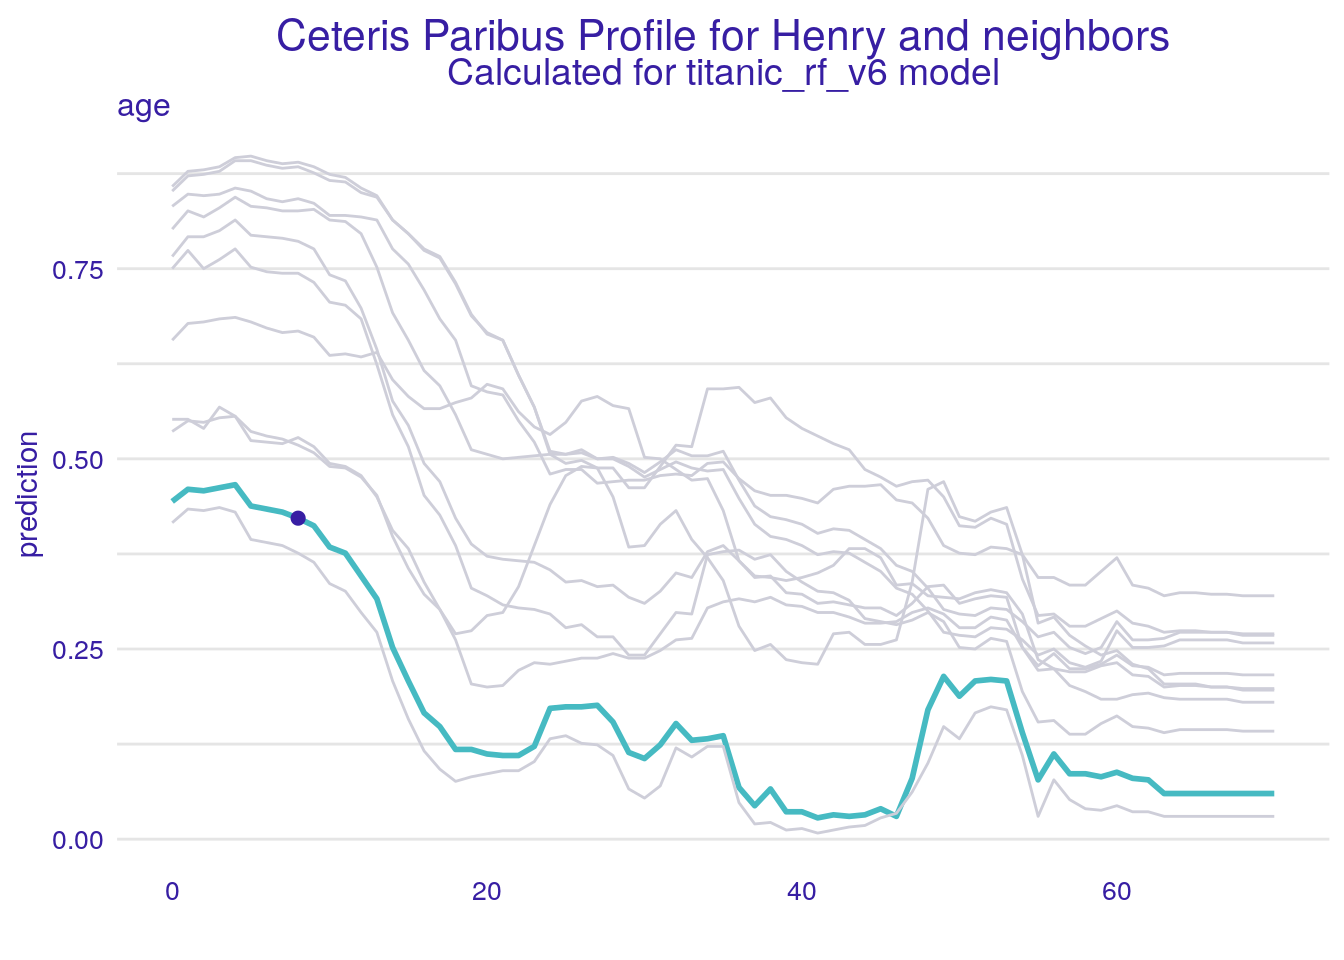
\includegraphics[width=0.7\linewidth]{PM_VEE_files/figure-latex/titanicCeterisParibus05-1} \end{center}

To construct the local-fidelity plot presented in Figure \ref{fig:localFidelityPlots}, we have got to add the information about the observed values of the dependent variable for the selected neighbors. Toward this aim, we use the \texttt{y} argument in the \texttt{ceteris\_paribus()} function. The argument takes numerical values. Our binary dependent variable \texttt{survived} assumes values \texttt{yes/no}; to convert them to numerical values, we use the \texttt{survived\ ==\ "yes"} expression.

\begin{Shaded}
\begin{Highlighting}[]
\NormalTok{cp_henry_neighbors <-}\StringTok{ }\KeywordTok{ceteris_paribus}\NormalTok{(explain_rf_v6,}
\NormalTok{                          henry_neighbors, }
                          \DataTypeTok{y =}\NormalTok{ henry_neighbors}\OperatorTok{$}\NormalTok{survived }\OperatorTok{==}\StringTok{ "yes"}\NormalTok{,}
                          \DataTypeTok{variable_splits =} \KeywordTok{list}\NormalTok{(}\DataTypeTok{age =} \KeywordTok{seq}\NormalTok{(}\DecValTok{0}\NormalTok{,}\DecValTok{80}\NormalTok{,}\FloatTok{0.1}\NormalTok{)))}
\end{Highlighting}
\end{Shaded}

Finally, we add residuals to the plot by using the \texttt{show\_residuals()} function. As a result, we obtain the local-fidelity plot for \texttt{henry}.

\begin{Shaded}
\begin{Highlighting}[]
\KeywordTok{plot}\NormalTok{(cp_henry_neighbors, }\DataTypeTok{color =} \StringTok{'#ceced9'}\NormalTok{) }\OperatorTok{+}
\CommentTok{#  show_profiles(cp_henry, size = 2) + }
\StringTok{  }\KeywordTok{show_observations}\NormalTok{(cp_henry, }\DataTypeTok{variables =} \StringTok{"age"}\NormalTok{, }\DataTypeTok{size =} \DecValTok{5}\NormalTok{) }\OperatorTok{+}
\CommentTok{#  show_residuals(cp_henry_neighbors, variables = "age") +}
\StringTok{  }\KeywordTok{ggtitle}\NormalTok{(}\StringTok{"Local-fidelity plot for Henry"}\NormalTok{,}\StringTok{"Calculated for the titanic_rf_v6 model"}\NormalTok{)}
\end{Highlighting}
\end{Shaded}

\begin{center}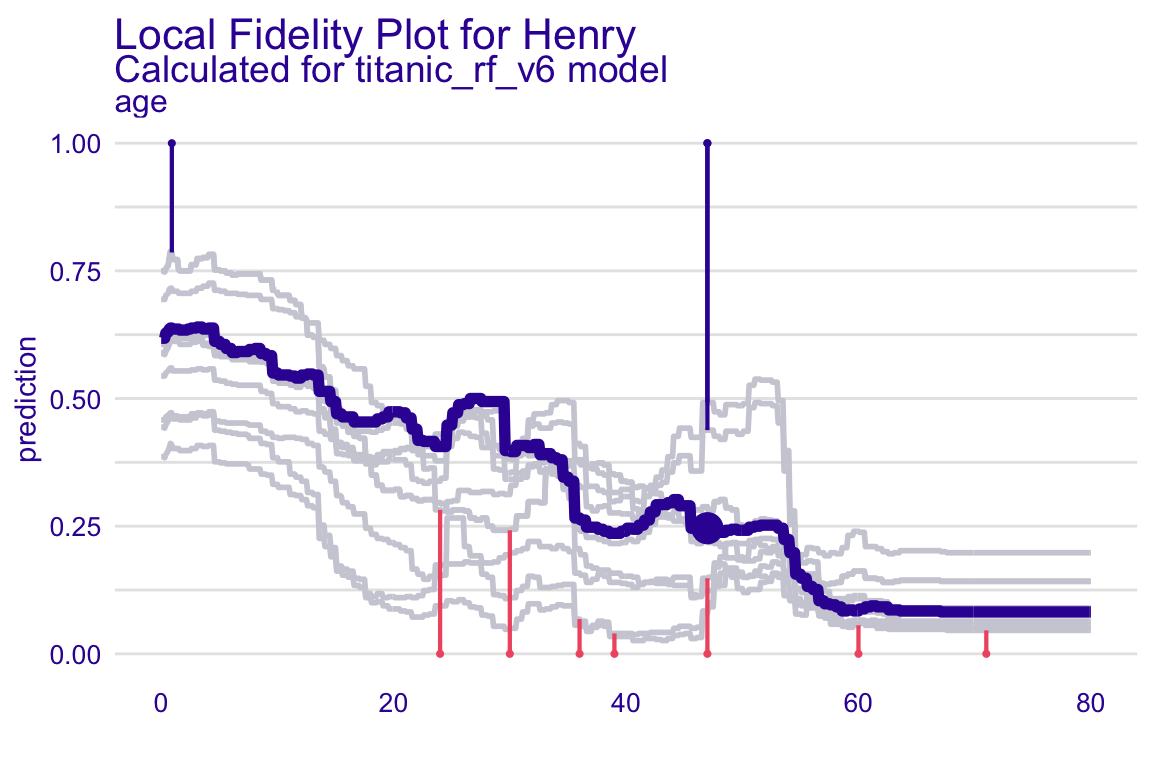
\includegraphics[width=0.7\linewidth]{PM_VEE_files/figure-latex/titanicCeterisParibus07-1} \end{center}

\hypertarget{breakDown}{%
\section{Break-down Plots for Additive Variable Attributions}\label{breakDown}}

In Chapter \ref{ceterisParibusOscillations}, we introduced a method for assessment of local variable-importance based on Ceteris-paribus (CP) profiles. The main disadvantage of this method is that the sum of the developed importance scores does not equal the final model prediction.

In this chapter we introduce Break-down (BD) plots, which offer a solution to this problem.
BD plots show ``variables attributions'' i.e., the decomposition of the difference between the single-instance and the average model predictions among the different explanatory variables.
Note that the method is similar to the \texttt{EXPLAIN} algorithm introduced in \citep{explainPaper} and implemented in the \texttt{ExplainPrediction} package \citep{explainPackage}.

\hypertarget{BDIntuition}{%
\subsection{Intuition}\label{BDIntuition}}

The underlying idea is to calculate contribution of an explanatory variable to model's prediction as a shift in the expected model response after conditioning on other variables.

The idea is illustrated in Figure \ref{fig:BDPrice4}. Consider the prediction for \texttt{johny\_d} for the random-forest model (see Section \ref{model-titanic-rf}) for the Titanic data. Panel A shows distribution of model predictions. The row \texttt{all\ data} shows the distribution of the predictions for the entire dataset. The red dot indicates the average and it is an estimate of the expected model prediction \(E_X[f(X)]\) over the distribution of all explanatory variables.

To evaluate the contribution of the explanatory variables to the particular instance prediction, we consider the predictions when fixing the values of the variables. For instance, the row \texttt{class=1st} in Panel A of Figure \ref{fig:BDPrice4} presents the distribution of the predictions obtained when the value of the \texttt{class} variable has been fixed to the \texttt{1st} class. Again, the red dot indicates the average of the predictions. The next row (\texttt{age=8}) shows the distribution and the average predictions with the value of variable \texttt{class} set to \texttt{1st} and \texttt{age} set to \texttt{8}, and so on. The last row corresponds to the prediction for \texttt{model\ response\ for}johny\_d`.

The black lines in Panel A show how the inidividual predictions change after the value of the \(j\)-th variable has been replaced by the value indicated in the name of the row.

Eventually, however, we may be interested in the average predictions, as indicated in Panel B of Figure \ref{fig:BDPrice4}, or even only in the changes of the averages, as shown in Panel C. In Panel C, positive changes are presented with green bars, while negative differences are marked with red bar. The changes sum up to the final prediction, which is illustrated by the violet bar at the bottom of Panel C.

What can be learned from Break-down plots? In this case we have concise summary of effects of particular variables on expected model response.
First, we see that average model response is 23.5 percent. These are odds of survival averaged over all people on Titanic. Note that it is not the fraction of people that survived, but the average model response, so for different models one can get different averages.
The model prediction for Johny D is 42.2 percent. It is much higher than an average prediction. Two variables that influence this prediction the most are class (=1st) and age (=8). Setting these two variables increase average model prediction by 33.5 percent points. Values in all other variables have rather negative effect. Low fare and being a male diminish odds of survival predicted by the model. Other variables do not change model predictions that much.
Note that value of variable attribution depends on the value not only a variable itself. In this example the \texttt{embarked\ =\ Southampton} has small effect on average model prediction. It may be because the variable \texttt{embarked} is not important or it is possible that variable \texttt{embarked} is important but \texttt{Southampton} has an average effect out of all other possible values of the \texttt{embarked} variable.

\begin{figure}

{\centering 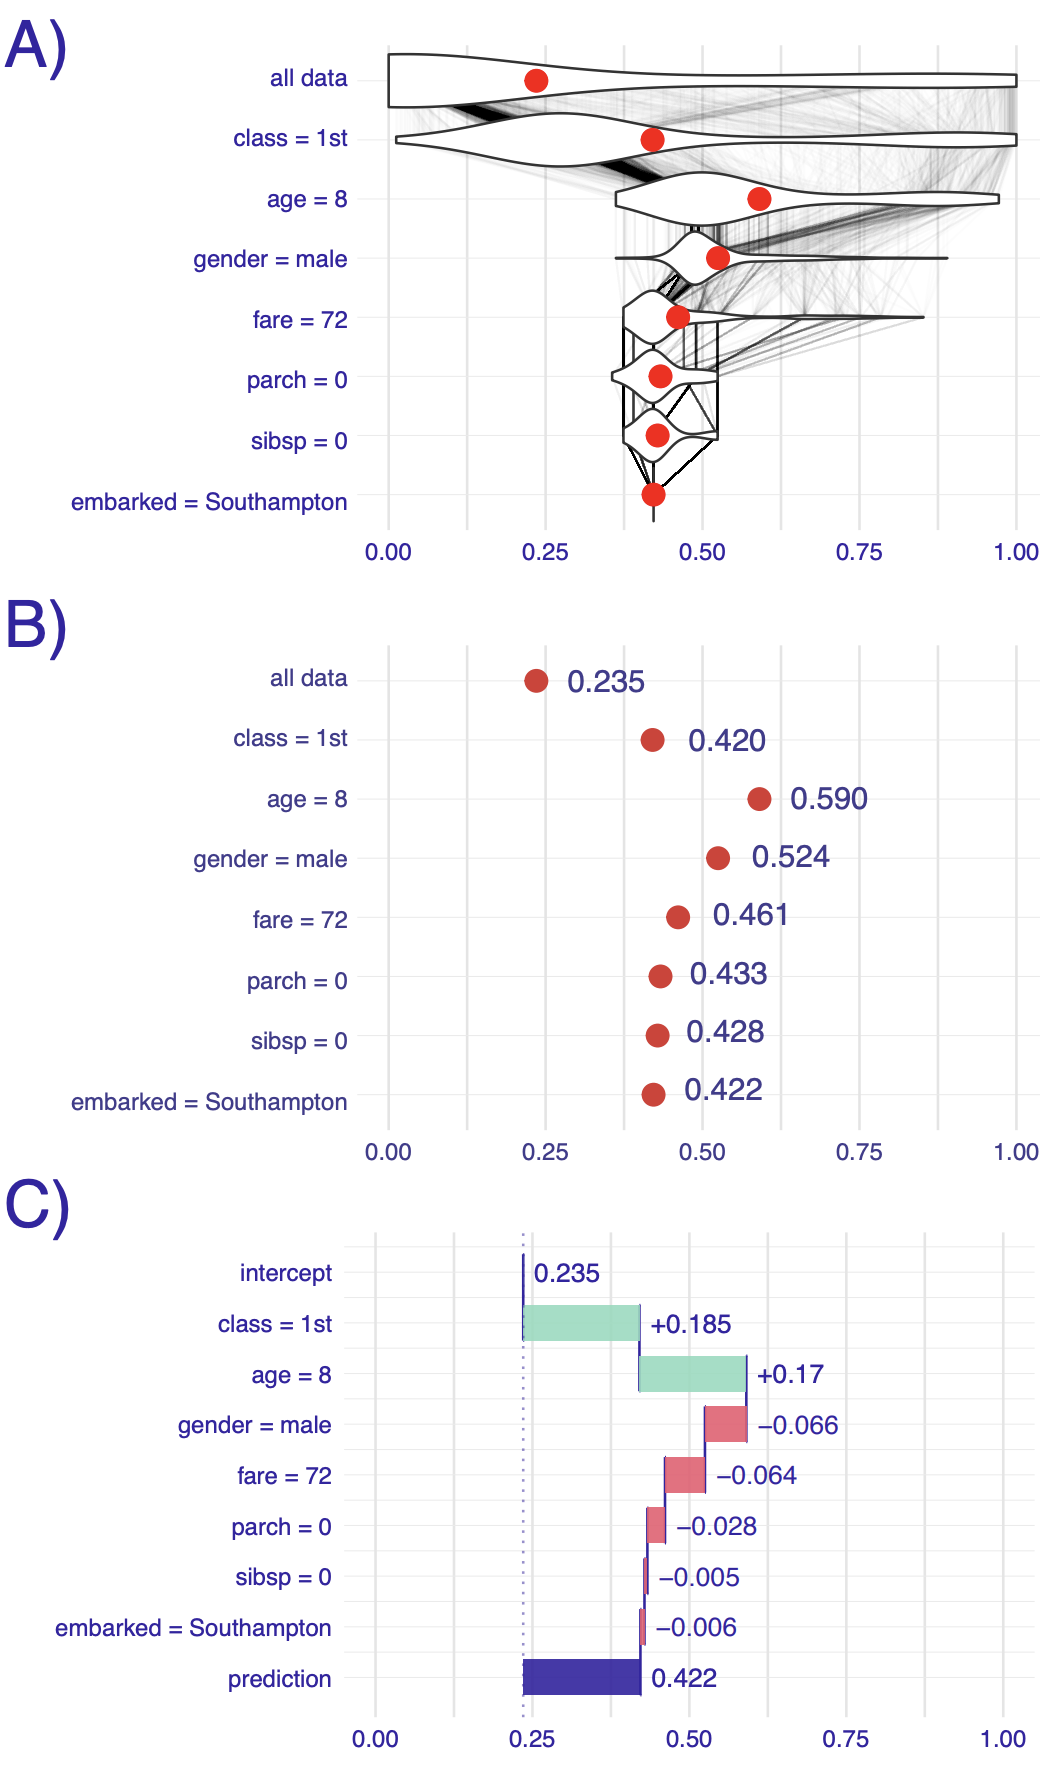
\includegraphics[width=0.8\linewidth]{figure/break_down_distr} 

}

\caption{(fig:BDPrice4) Break-down plots show how the contribution of individual explanatory variables change the average model prediction to the prediction for a single instance (observation). Panel A) The first row shows the distribution and the average (red dot) of model predictions for all data. The next rows show the dirstribution and the average of the predictions when fixing values of subseqeunt explanatory variables. The last row shows the prediction for a particular instance of interest. B) Red dots indicate the average predictions from Panel B. C) The green and red bars indicate, resspectively, positive and negative changes in the average predictions (variable contributions). }\label{fig:BDPrice4}
\end{figure}

\hypertarget{BDMethod}{%
\subsection{Method}\label{BDMethod}}

First, let's see how variable attribution works for linear models.

\hypertarget{break-down-for-linear-models}{%
\subsubsection{Break-down for linear models}\label{break-down-for-linear-models}}

Assume a classical linear model for response \(Y\) with \(p\) explanatory variables collected in the vector \(X = (X^1, X^2, \ldots, X^p)\) and coefficients \(\beta = (\beta^0, \beta^1, .., \beta^p)\), where \(\beta^0\) is the intercept. The prediction for \(Y\) at point \(X=x=(x^1, x^2, \ldots, x^p)\) is given by the expected value of \(Y\) conditional on \(X=x\). For a linear model, the expected value is given by the following linear combination:

\[
E_Y(Y | x) = f(x) = \beta^0 + x^1 \beta^1 + \ldots + x^p \beta^p.
\]\\
We are interested in the contribution of the \(i\)-th explanatory variable to model prediction \(f(x_*)\) for a single observation described by \(x_*\). In this case, the contribution is equal to \(x_*^i\beta^i\), because the \(i\)-th variable occurs only in this term. As it will become clear in the sequel, it is easier to interpret the variable's contribution if \(x^i\) is is centered by subtracting a constant \(\hat x^i\) (usually, the mean of \(x^i\)). This leads the following, intuitive formula for the variable attribution:
\[
v(i, x_*) = \beta_i (x^i_* - \hat x^i).
\]

We want to calculate \(v(f, x_*, i)\), which is the contribution of the \(i\)-th explanatory variable to the prediction of model \(f()\) at point \(x_*\). Assume that \(E_Y(Y | x_*) \approx f(x_*)\), where \(f(x_*)\) is the value of the model at \(x_*\). A possible approach to define \(v(f, x_*, i)\) is to measure how much the expected model response changes after conditioning on \(x^i_*\):
\[
v(i, x_*) = E_Y(Y | x_*) - E_{X^i}\{E_Y[Y | (x^1_*,\ldots,x^{i-1}_*,X^i,x^{i+1}_*,x^p_*)]\}\approx f(x_*) - E_{X^i}[f(x^{-i}_*)],
\]
where \(x^{-i}_*\) indicates that variable \(X^i\) in vector \(x_*\) is treated as random. For the classical linear model, if the explanatory variables are independent, \(v(f, x_*, i)\) can be expressed as follows:
\[
v(i, x_*) = f(x_*) - E_{X^i}[f(x^{-i}_*)] = \beta^0 + x^1_* \beta^1 + \ldots + x^p_* \beta^p - E_{X^i}[\beta^0 + x^1_* \beta^1 + \ldots +\beta^i X^i \ldots + x^p_* \beta^p] = \beta^i[x_*^i - E_{X^i}(X^i)].
\]
In practice, given a dataset, the expected value of \(X_i\) can be estimated by the sample mean \(\bar x_i\). This leads to\\
\[
v(i, x_*) = \beta_i (x_*^i - \bar x^i).
\]
Note that the linear-model-based prediction may be re-expressed in the following way:
\[
f(x_*) = [\beta^0 + \bar x^1 \beta^1 + ... + \bar x^p \beta^p] + [(x^1_* - \bar x^1) \beta^1 + ... + (x^p_* - \bar x^p) \beta^p] 
\]
\[
 \equiv [average \ prediction] + \sum_{j=1}^p v(i, x_*).
\]
Thus, the contributions of the explanatory variables are the differences between the model prediction for \(x_*\) and the average prediction.

** NOTE for careful readers **

Obviously, sample mean \(\bar x^i\) is an estimator of the expected value \(E_{X^i}(X^i)\), calculated using a dataset. For the sake of simplicity we do not emphasize these differences in the notation. Also, we ignore the fact that, in practice, we never know the model coefficients and we work with an estimated model.

\hypertarget{break-down-for-general-case}{%
\subsubsection{Break-down for general case}\label{break-down-for-general-case}}

Again, let \(v(j, x_*)\) denote the variable-importance measure of the \(j\)-th variable and instance \(x_*\), i.e., the contribution of the \(j\)-th variable to prediction at \(x_*\).

We would like the sum of the variable-importance measures for all explanatory variables to be equal to the instance prediction (property called \emph{local accuracy}), so that
\[
f(x_*) = v_0 + \sum_{j=1}^p v(j, x_*),
\]
where \(v_0\) denotes the average model response. If we re-write the equation above as follows:
\[
E_X[f(X)|X^1 = x^1_*, \ldots, X^p = x^p_*] = E_X[f(X)] + \sum_{j=1}^p v(j, x_*),
\]
then a natural proposal for \(v(j, x_*)\) is

\[
v(j, x_*) = E_X[f(X) | X^1 = x^1_*, \ldots, X^j = x^j_*] - E_X[f(X) | X^1 = x^1_*, \ldots, X^{j-1} = x^{j-1}_*]. 
\]
In other words, the contribution of the \(j\)-th variable is the difference between the expected value of the prediction conditional on setting the values of the first \(j\) variables equal to their values in \(x_*\) and the expected value conditional on setting the values of the first \(j-1\) variables equal to their values in \(x_*\).

Note that the definition does imply the dependence of \(v(j, x_*)\) on the order of the explanatory variables that is reflected in their indices.

To consider more general cases, let \(J\) denote a subset of \(K\) (\(K\leq p\)) indices from \(\{1,2,\ldots,p\}\), i.e., \(J=\{j_1,j_2,\ldots,j_K\}\) where each \(j_k \in \{1,2,\ldots,p\}\). Furthermore, let \(L\) denote another subset of \(M\) (\(M \leq p-K\)) indices from \({1,2,\ldots,p}\) distinct from \(J\). That is, \(L=\{l_1,l_2,\ldots,l_M\}\) where each \(l_m \in \{1,2,\ldots,p\}\) and \(J \cap L = \emptyset\). Let us define now

\begin{eqnarray}
\Delta^{L|J}(x_*) &\equiv& E_X[f(X) | X^{l_1} = x_*^{l_1},\ldots,X^{l_M} = x_*^{l_M},X^{j_1} = x_*^{j_1},\ldots,X^{j_K} = x_*^{j_K}]\\
&-& E_X[f(X) | X^{j_1} = x_*^{j_1},\ldots,X^{j_K} = x_*^{j_K}].
\end{eqnarray}

In other words, \(\Delta^{L|J}(x_*)\) is the change between the expected prediction when setting the values of the explanatory variables with indices from the set \(J \cup L\) equal to their values in \(x_*\) and the expected prediction conditional on setting the values of the explanatory variables with indices from the set \(J\) equal to their values in \(x_*\).

In particular, for the \(l\)-th explanatory variable, let
\begin{eqnarray}
\Delta^{l|J}(x_*) \equiv \Delta^{\{l\}|J}(x_*) &=& E_X[f(X) | X^{l} = x_*^{l},X^{j_1} = x_*^{j_1},\ldots,X^{j_K} = x_*^{j_K}]\\
&-& E_X[f(X) | X^{j_1} = x_*^{j_1},\ldots,X^{j_K} = x_*^{j_K}].
\end{eqnarray}

Thus, \(\Delta^{l|J}\) is the change between the expected prediction when setting the values of the explanatory variables with indices from the set \(J \cup \{l\}\) equal to their values in \(x_*\) and the expected prediction conditional on setting the values of the explanatory variables with indices from the set \(J\) equal to their values in \(x_*\). Note that, if \(J=\emptyset\), then
\[
\Delta^{l|\emptyset}(x_*) = E_X[f(X) | X^{l} = x_*^{l}] - E_X[f(X)].
\]
It follows that
\[
v(j, x_*) = \Delta^{j|\{1,  ..., j-1\}}(x_*).
\]
Unfortunately, for non-additive models (that include interactions), the value of so-defined variable-importance measure depends on the order, in which one sets the values of the explanatory variables. Figure \ref{fig:ordering} presents an example.
We fit the random forest model to predict whether a passenger survived or not, then, we explain the model's prediction for a 2-year old boy that travels in the second class. The model predicts survival with a probability of \(0.964\). We would like to explain this probability and understand which factors drive this prediction. Consider two explanations.

\textbf{Explanation 1:}
The passenger is a boy, and this feature alone decreases the chances of survival. He traveled in the second class which also lower survival probability.
Yet, he is very young, which makes odds higher. The reasoning behind such an explanation on this level is that most passengers in the second class are adults, therefore a kid from the second class has high chances of survival.

\textbf{Explanation 2:}
The passenger is a boy, and this feature alone decreases survival probability.
However, he is very young, therefore odds are higher than adult men. Explanation in the last step says that he traveled in the second class, which make odds of survival even more higher. The interpretation of this explanation is that most kids are from the third class and being a child in the second class should increase chances of survival.

Note that the effect of \emph{the second class} is negative in explanations for scenario 1 but positive in explanations for scenario 2.

\begin{figure}

{\centering 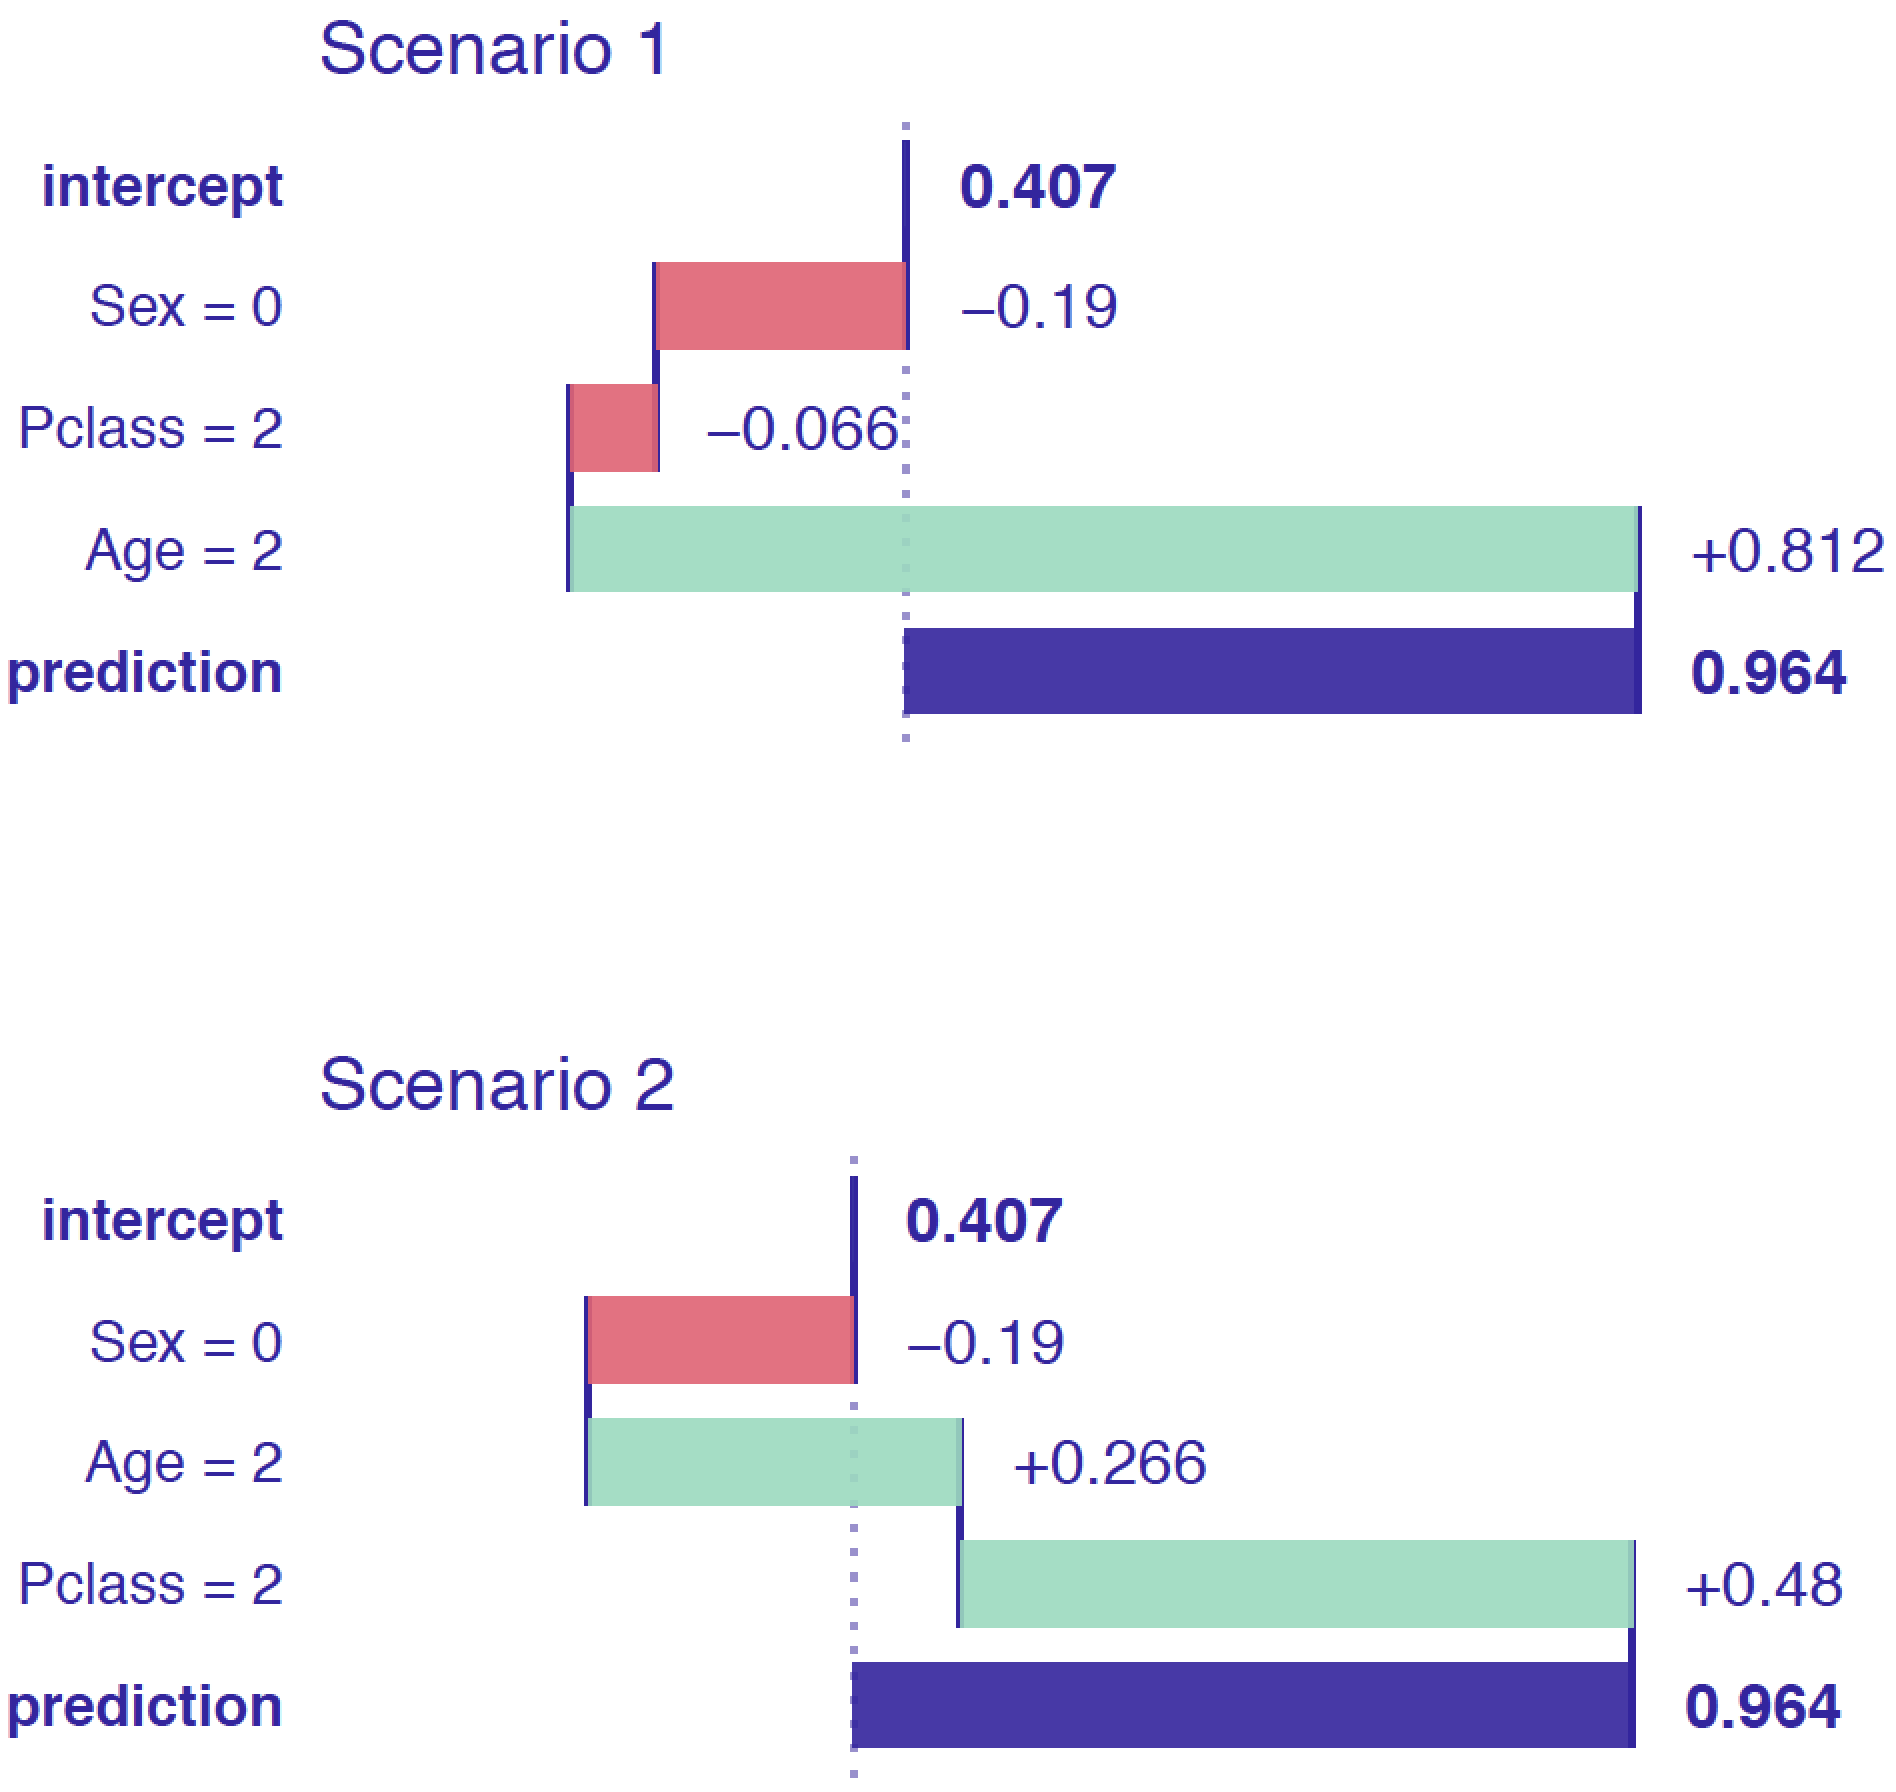
\includegraphics[width=0.7\linewidth]{figure/ordering} 

}

\caption{(fig:ordering) An illustration of the order-dependence of the variable-contribution values. Two *Break-down* explanations for the same observation from Titanic data set. The underlying model is a random forest. Scenarios differ due to the order of variables in *Break-down* algorithm. Blue bar indicates the difference between the model's prediction for a particular observation and an average model prediction. Other bars show contributions of variables. Red color means a negative effect on the survival probability, while green color means a positive effect. Order of variables on the y-axis corresponds to their sequence used in *Break-down*~algorithm.}\label{fig:ordering}
\end{figure}

There are three approaches that can be used to address the issue of the dependence of \(v(j, x_*)\) on the order, in which one sets the values of the explanatory variables.

In the first approach, one chooses an ordering according to which the variables with the largest contributions are selected first. In this chapter, we describe a heuristic behind this approach.

In the second approach, one identifies the interactions that cause a difference in variable-importance measure for different orderings and focuses on those interactions. This approach is discussed in Chapter \ref{iBreakDown}.

Finally, one can calculate an average value of the variance-importance measure across all possible orderings. This approach is presented in Chapter \ref{shapley}.

To choose an ordering according to which the variables with the largest contributions are selected first, one can apply a two-step procedure. In the first step, the explanatory variables are ordered. In the second step, the conditioning is applied according to the chosen order of variables.

In the first step, the ordering is chosen based on the decreasing value of the scores equal to \(|\Delta^{k|\emptyset}|\). Note that the absolute value is needed, because the variable contributions can be positive or negative. In the second step, the variable-importance measure for the \(j\)-th variable is calculated as
\[
v(j, x_*) = \Delta ^{j|J},
\]
where
\[
J = \{k: |\Delta^{k|\emptyset}| < |\Delta^{j|\emptyset}|\},
\]
that is, \(J\) is the set of indices of explanatory variables that have scores \(|\Delta^{k|\emptyset}|\) smaller than the corresponding score for variable \(j\).

The time complexity of theeach of the two steps of the procedure is \(O(p)\), where \(p\) is the number of explanatory variables.

\hypertarget{BDExample}{%
\subsection{Example: Titanic data}\label{BDExample}}

Let us consider the random-forest model \texttt{titanic\_rf\_v6} (see Section \ref{model-titanic-rf} and passenger \texttt{johny\_d} (see Section \ref{predictions-titanic}) as the instance of interest in the Titanic data.

The average of model predictions for all passengers is equal to \(v_0 = 0.2353095\). Table \ref{tab:titanicBreakDownDeltas} presents the scores \(|\Delta^{j|\emptyset}|\) and the expected values \(E[f(X | X^j = x^j_*)]\). Note that \(\Delta^{j|\emptyset}=E[f(X) | X^j = x^j_*]-v_0\) and, since for all variables \(E[f(X) | X^j = x^j_*]>v_0\), we have got \(E[f(X | X^j = x^j_*)]=|\Delta^{j|\emptyset}|+v_0\).

\begin{longtable}[]{@{}lrr@{}}
\caption{\label{tab:titanicBreakDownDeltas} Expected values \(E[f(X) | X^j = x^j_*]\) and scores \(|\Delta^{j|\emptyset}|\) for the random-forest model \texttt{titanic\_rf\_v6} for the Titanic data and \texttt{johny\_d}. The scores are sorted in the decreasing order.}\tabularnewline
\toprule
variable \(j\) & \(E[f(X) | X^j = x^j_*]\) & \(|\Delta^{j|\emptyset}|\)\tabularnewline
\midrule
\endfirsthead
\toprule
variable \(j\) & \(E[f(X) | X^j = x^j_*]\) & \(|\Delta^{j|\emptyset}|\)\tabularnewline
\midrule
\endhead
age & 0.7407795 & 0.5051210\tabularnewline
class & 0.6561034 & 0.4204449\tabularnewline
fare & 0.6141968 & 0.3785383\tabularnewline
sibsp & 0.4786182 & 0.2429597\tabularnewline
parch & 0.4679240 & 0.2322655\tabularnewline
embarked & 0.4602620 & 0.2246035\tabularnewline
gender & 0.3459458 & 0.1102873\tabularnewline
\bottomrule
\end{longtable}

Based on the ordering defined by the scores \(|\Delta^{j|\emptyset}|\) from Table \ref{tab:titanicBreakDownDeltas}, we can compute the variable-importance measures based on the sequential contributions \(\Delta^{j|J}\). The computed values are presented in Table \ref{tab:titanicBreakDownDeltasConseq}.

\begin{longtable}[]{@{}lrr@{}}
\caption{\label{tab:titanicBreakDownDeltasConseq} Variable-importance measures \(\Delta^{j|\{1,\ldots,j\}}\) for the random-forest model \texttt{titanic\_rf\_v6} for the Titanic data and \texttt{johny\_d} computed by using the ordering of variables defined in Table \ref{tab:titanicBreakDownDeltas}.}\tabularnewline
\toprule
\begin{minipage}[b]{0.44\columnwidth}\raggedright
variable \(j\)\strut
\end{minipage} & \begin{minipage}[b]{0.23\columnwidth}\raggedleft
\(E[f(X) | X^{\{1,\ldots,j\}} = x^{\{1,\ldots,j\}}_*)]\)\strut
\end{minipage} & \begin{minipage}[b]{0.25\columnwidth}\raggedleft
\(\Delta^{j|\{1,\ldots,j\}}\)\strut
\end{minipage}\tabularnewline
\midrule
\endfirsthead
\toprule
\begin{minipage}[b]{0.44\columnwidth}\raggedright
variable \(j\)\strut
\end{minipage} & \begin{minipage}[b]{0.23\columnwidth}\raggedleft
\(E[f(X) | X^{\{1,\ldots,j\}} = x^{\{1,\ldots,j\}}_*)]\)\strut
\end{minipage} & \begin{minipage}[b]{0.25\columnwidth}\raggedleft
\(\Delta^{j|\{1,\ldots,j\}}\)\strut
\end{minipage}\tabularnewline
\midrule
\endhead
\begin{minipage}[t]{0.44\columnwidth}\raggedright
intercept\strut
\end{minipage} & \begin{minipage}[t]{0.23\columnwidth}\raggedleft
0.2353095\strut
\end{minipage} & \begin{minipage}[t]{0.25\columnwidth}\raggedleft
0.2353095\strut
\end{minipage}\tabularnewline
\begin{minipage}[t]{0.44\columnwidth}\raggedright
age = 8\strut
\end{minipage} & \begin{minipage}[t]{0.23\columnwidth}\raggedleft
0.5051210\strut
\end{minipage} & \begin{minipage}[t]{0.25\columnwidth}\raggedleft
0.2698115\strut
\end{minipage}\tabularnewline
\begin{minipage}[t]{0.44\columnwidth}\raggedright
class = 1st\strut
\end{minipage} & \begin{minipage}[t]{0.23\columnwidth}\raggedleft
0.5906969\strut
\end{minipage} & \begin{minipage}[t]{0.25\columnwidth}\raggedleft
0.0855759\strut
\end{minipage}\tabularnewline
\begin{minipage}[t]{0.44\columnwidth}\raggedright
fare = 72\strut
\end{minipage} & \begin{minipage}[t]{0.23\columnwidth}\raggedleft
0.5443561\strut
\end{minipage} & \begin{minipage}[t]{0.25\columnwidth}\raggedleft
-0.0463407\strut
\end{minipage}\tabularnewline
\begin{minipage}[t]{0.44\columnwidth}\raggedright
gender = male\strut
\end{minipage} & \begin{minipage}[t]{0.23\columnwidth}\raggedleft
0.4611518\strut
\end{minipage} & \begin{minipage}[t]{0.25\columnwidth}\raggedleft
-0.0832043\strut
\end{minipage}\tabularnewline
\begin{minipage}[t]{0.44\columnwidth}\raggedright
embarked = Southampton\strut
\end{minipage} & \begin{minipage}[t]{0.23\columnwidth}\raggedleft
0.4584422\strut
\end{minipage} & \begin{minipage}[t]{0.25\columnwidth}\raggedleft
-0.0027096\strut
\end{minipage}\tabularnewline
\begin{minipage}[t]{0.44\columnwidth}\raggedright
sibsp = 0\strut
\end{minipage} & \begin{minipage}[t]{0.23\columnwidth}\raggedleft
0.4523398\strut
\end{minipage} & \begin{minipage}[t]{0.25\columnwidth}\raggedleft
-0.0061024\strut
\end{minipage}\tabularnewline
\begin{minipage}[t]{0.44\columnwidth}\raggedright
parch = 0\strut
\end{minipage} & \begin{minipage}[t]{0.23\columnwidth}\raggedleft
0.4220000\strut
\end{minipage} & \begin{minipage}[t]{0.25\columnwidth}\raggedleft
-0.0303398\strut
\end{minipage}\tabularnewline
\begin{minipage}[t]{0.44\columnwidth}\raggedright
prediction\strut
\end{minipage} & \begin{minipage}[t]{0.23\columnwidth}\raggedleft
0.4220000\strut
\end{minipage} & \begin{minipage}[t]{0.25\columnwidth}\raggedleft
0.4220000\strut
\end{minipage}\tabularnewline
\bottomrule
\end{longtable}

Results from Table \ref{tab:titanicBreakDownDeltasConseq} are presented as a waterfall plot in Figure \ref{fig:BDjohnyExample}.

\textbackslash{}begin\{figure\}

\{\centering 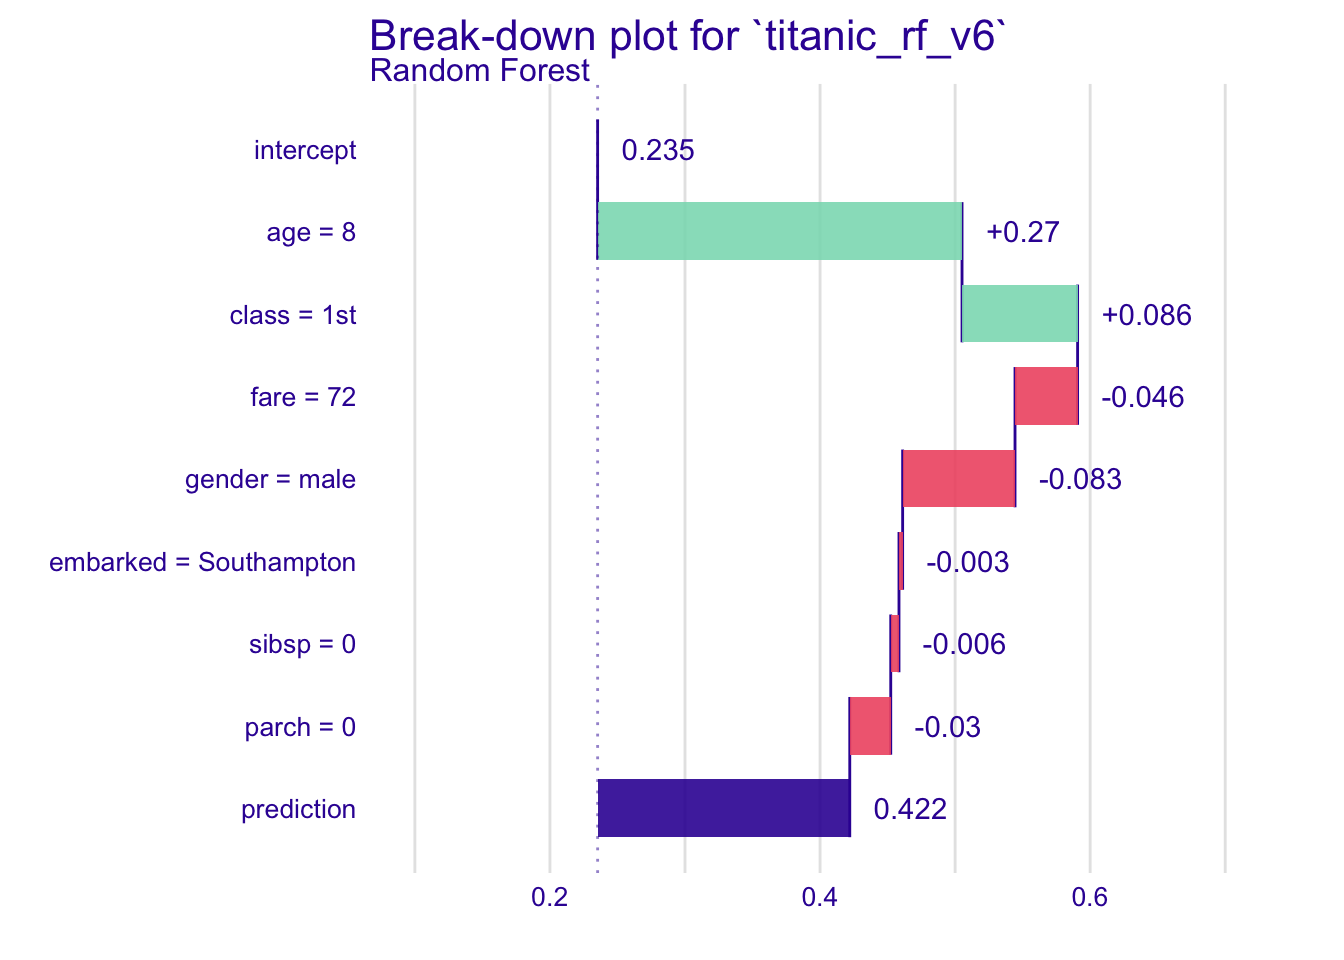
\includegraphics[width=0.7\linewidth]{PM_VEE_files/figure-latex/BDjohnyExample-1}

\}

\textbackslash{}caption\{(fig:BDjohnyExample) Break-down plot for the \texttt{titanic\_rf\_v6} model and \texttt{johny\_d} for the Titanic data.\}\label{fig:BDjohnyExample}
\textbackslash{}end\{figure\}

\hypertarget{BDProsCons}{%
\subsection{Pros and cons}\label{BDProsCons}}

Break-down plots offer a model-agnostic approach that can be applied to any predictive model that returns a single number. The approach offers several advantages. The plots are easy to understand. They are compact; results for many variables may be presented in a small space. The approach reduces to an intuitive interpretation for the generalized-linear models. Numerical complexity of the Break-down algorithm is linear in the number of explanatory variables.

Break-down plots for non-additive models may be misleading, as they show only the additive contributions. An important issue is the choice of the ordering of the explanatory variables that is used in the calculation of the variable-importance measures. Also, for models with a large number of variables, the Break-down plot may be complex and include many variables with small contributions to the instance prediction.

\hypertarget{BDR}{%
\subsection{Code snippets for R}\label{BDR}}

In this section, we present key features of the \texttt{iBreakDown} R package \citep{iBreakDownRPackage} which is a part of the \texttt{DrWhy.AI} universe. The package covers all methods presented in this chapter. It is available on CRAN and GitHub. More details and examples can be found at \url{https://modeloriented.github.io/iBreakDown/}.

For illustration purposes, we use the \texttt{titanic\_rf\_v6} random-forest model for the Titanic data developed in Section \ref{model-titanic-rf}. Recall that it is developed to predict the probability of survival from sinking of Titanic. Instance-level explanations are calculated for a single observation: \texttt{johny\_d} - an 8-year-old passenger that travelled in the 1st class.

\texttt{DALEX} explainers for the model and the \texttt{jonhy\_d} data are retrieved via \texttt{archivist} hooks as listed in Section \ref{ListOfModelsTitanic}.

\begin{Shaded}
\begin{Highlighting}[]
\KeywordTok{library}\NormalTok{(}\StringTok{"randomForest"}\NormalTok{)}
\NormalTok{explain_rf_v6 <-}\StringTok{ }\NormalTok{archivist}\OperatorTok{::}\KeywordTok{aread}\NormalTok{(}\StringTok{"pbiecek/models/9b971"}\NormalTok{)}

\KeywordTok{library}\NormalTok{(}\StringTok{"DALEX"}\NormalTok{)}
\NormalTok{johny_d <-}\StringTok{ }\NormalTok{archivist}\OperatorTok{::}\KeywordTok{aread}\NormalTok{(}\StringTok{"pbiecek/models/e3596"}\NormalTok{)}
\NormalTok{johny_d}
\end{Highlighting}
\end{Shaded}

\hypertarget{basic-use-of-the-break_down-function}{%
\subsubsection{\texorpdfstring{Basic use of the \texttt{break\_down()} function}{Basic use of the break\_down() function}}\label{basic-use-of-the-break_down-function}}

The \texttt{iBreakDown::break\_down()} function calculates the variable-importance measures for a selected model and the instance of interest. The result of applying the \texttt{break\_down()} function is a data frame containg the calculated measures. In the simplest call, the function requires only two arguments: the model explainers and the data frame for the instance of interest. The call below essentailly re-creates the variable-importance values (\(\Delta^{j|\{1,\ldots,j\}}\)) presented in Table \ref{tab:titanicBreakDownDeltasConseq}.

\begin{Shaded}
\begin{Highlighting}[]
\KeywordTok{library}\NormalTok{(}\StringTok{"iBreakDown"}\NormalTok{)}
\NormalTok{bd_rf <-}\StringTok{ }\KeywordTok{break_down}\NormalTok{(explain_rf_v6, johny_d)}
\NormalTok{bd_rf}
\end{Highlighting}
\end{Shaded}

\begin{verbatim}
##                                          contribution
## Random Forest v6: intercept                     0.235
## Random Forest v6: age = 8                       0.270
## Random Forest v6: class = 1st                   0.086
## Random Forest v6: fare = 72                    -0.046
## Random Forest v6: gender = male                -0.083
## Random Forest v6: embarked = Southampton       -0.003
## Random Forest v6: sibsp = 0                    -0.006
## Random Forest v6: parch = 0                    -0.030
## Random Forest v6: prediction                    0.422
\end{verbatim}

Applying the generic \texttt{plot()} function to the object resulting from the application of the \texttt{break\_down()} function creates a BD plot. In this case, it is the plot from Figure \ref{fig:BDjohnyExample}.
.

\begin{Shaded}
\begin{Highlighting}[]
\KeywordTok{plot}\NormalTok{(bd_rf) }
\end{Highlighting}
\end{Shaded}

\begin{figure}

{\centering 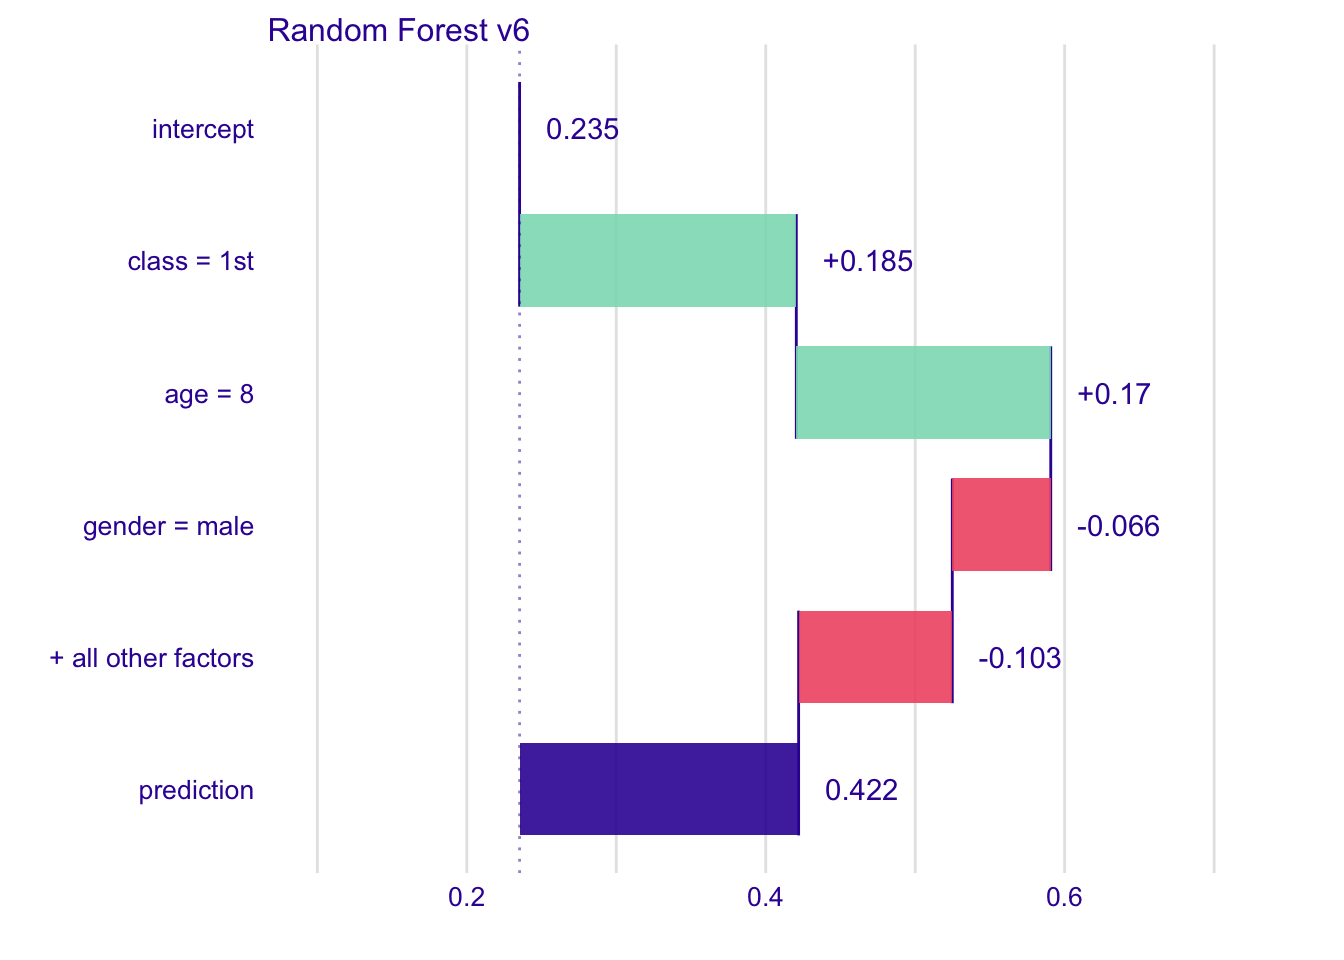
\includegraphics[width=0.7\linewidth]{PM_VEE_files/figure-latex/unnamed-chunk-34-1} 

}

\caption{Generic plot() function for the break down method.}\label{fig:unnamed-chunk-34}
\end{figure}

\hypertarget{advanced-use-of-the-break_down-function}{%
\subsubsection{\texorpdfstring{Advanced use of the \texttt{break\_down()} function}{Advanced use of the break\_down() function}}\label{advanced-use-of-the-break_down-function}}

The function \texttt{break\_down()} allows more arguments. The most commonly used are:

\begin{itemize}
\tightlist
\item
  \texttt{x} - a wrapper over a model created with function \texttt{DALEX::explain()},
\item
  \texttt{new\_observation} - an observation to be explained is should be a data frame with structure that matches the training data,
\item
  \texttt{order} - a vector of characters (column names) or integers (column indexes) that specify order of explanatory variables that is used for computing the variable-importance measures. If not specified (default), then a one-step heuristic is used to determine the order,
\item
  \texttt{keep\_distributions} - a logical value; if \texttt{TRUE}, then additional diagnostic information about conditional distributions is stored in the resulting object and can be plotted with the generic \texttt{plot()} function.
\end{itemize}

In what follows we illustrate the use of the arguments.

First, we will specify the ordering of the explanatory variables. Toward this end we can use integer indexes or variable names. The latter option is prerferable in most cases because of transparency. Additionally, to reduce clutter in the plot, we set \texttt{max\_features\ =\ 3} argument in the \texttt{plot()} function.

\begin{Shaded}
\begin{Highlighting}[]
\KeywordTok{library}\NormalTok{(}\StringTok{"iBreakDown"}\NormalTok{)}
\NormalTok{bd_rf_order <-}\StringTok{ }\KeywordTok{break_down}\NormalTok{(explain_rf_v6,}
\NormalTok{                 johny_d,}
                 \DataTypeTok{order =} \KeywordTok{c}\NormalTok{(}\StringTok{"class"}\NormalTok{, }\StringTok{"age"}\NormalTok{, }\StringTok{"gender"}\NormalTok{, }\StringTok{"fare"}\NormalTok{, }\StringTok{"parch"}\NormalTok{, }\StringTok{"sibsp"}\NormalTok{, }\StringTok{"embarked"}\NormalTok{))}
\KeywordTok{plot}\NormalTok{(bd_rf_order, }\DataTypeTok{max_features =} \DecValTok{3}\NormalTok{) }
\end{Highlighting}
\end{Shaded}

\begin{figure}

{\centering 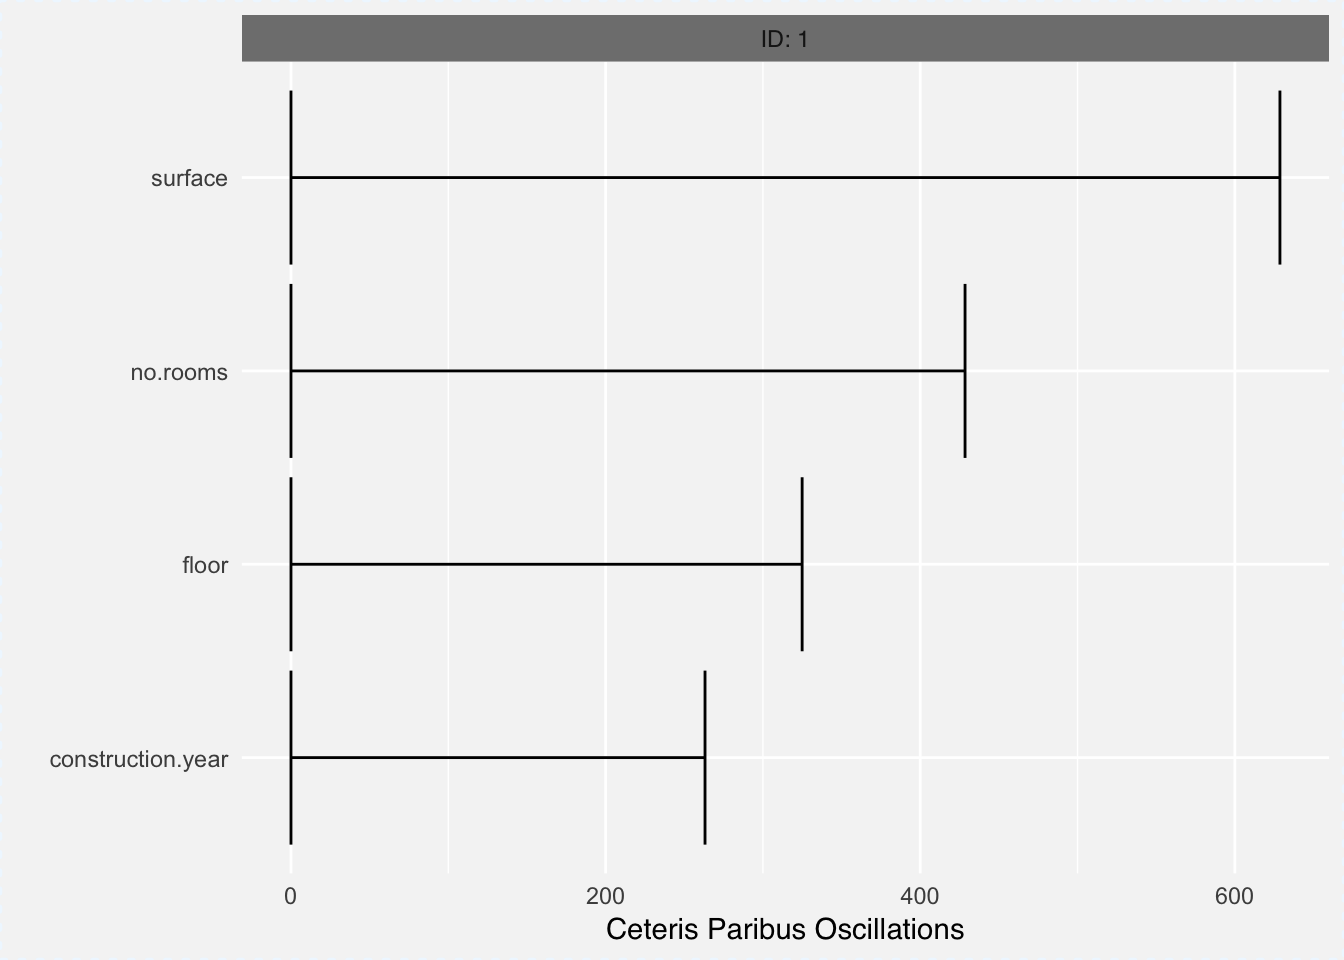
\includegraphics[width=0.7\linewidth]{PM_VEE_files/figure-latex/unnamed-chunk-35-1} 

}

\caption{Break Down plot limited to top three features.}\label{fig:unnamed-chunk-35}
\end{figure}

We can use the\texttt{keep\_distributions\ =\ TRUE} argument to enrich the resulting object with additional information about conditional distributions. Subsequently, we can apply the \texttt{plot\_distributions\ =\ TRUE} argument in the \texttt{plot()} function to present the distributions as violin plots. Red dots in the plots indicate the average model predictions. Thin black lines between violin plots correspond to predictions for individual observations. They can be used to trace how model predictions change after consecutive conditionings.

\begin{Shaded}
\begin{Highlighting}[]
\NormalTok{bd_rf_distr <-}\StringTok{ }\KeywordTok{break_down}\NormalTok{(explain_rf_v6,}
\NormalTok{                 johny_d,}
                 \DataTypeTok{order =} \KeywordTok{c}\NormalTok{(}\StringTok{"class"}\NormalTok{, }\StringTok{"age"}\NormalTok{, }\StringTok{"gender"}\NormalTok{, }\StringTok{"fare"}\NormalTok{, }\StringTok{"parch"}\NormalTok{, }\StringTok{"sibsp"}\NormalTok{, }\StringTok{"embarked"}\NormalTok{),}
                 \DataTypeTok{keep_distributions =} \OtherTok{TRUE}\NormalTok{)}
\KeywordTok{plot}\NormalTok{(bd_rf_distr, }\DataTypeTok{plot_distributions =} \OtherTok{TRUE}\NormalTok{) }
\end{Highlighting}
\end{Shaded}

\begin{figure}

{\centering \includegraphics[width=0.7\linewidth]{PM_VEE_files/figure-latex/unnamed-chunk-36-1} 

}

\caption{Distributions for conditional conditionings.}\label{fig:unnamed-chunk-36}
\end{figure}

\hypertarget{iBreakDown}{%
\section{Break-down Plots for Models with Interactions (iBreak-down Plots)}\label{iBreakDown}}

In Chapter \ref{breakDown}, we presented a model-agnostic approach to evaluation of the importance of an explanatory variable for model predictions. An important issue is that, for models with interactions, the estimated value of the variable-importance measure depends on the ordering of the explanatory varaibles that is used when computing the measure.

In this chapter, we present an algorithm that addresses the issue. In particular, the algorithm identifies interactions between pairs of variables and takes them into account when constructing Break-down (BD) plots. In our presentation we focus on interactions that involve pairs of explanatory variables, but the algorithm can be easily extended to interactions involving a larger number of variables.

\hypertarget{iBDIntuition}{%
\subsection{Intuition}\label{iBDIntuition}}

An interation means that the effect of an explanatory variable depends on the value(s) of other variable(s). To illustrate such a situation, we will consider the Titanic dataset (see Section \ref{TitanicDataset}. For the sake of simplicity, we consider only two variables, \texttt{age} and \texttt{class}. In the data \texttt{age} is a continuous variable, but we will use a dichotomized version of it, with two levels: boys (0-16 years old) and adults (17+ years old). Also, we will consider just two classess: the 2nd and ``other''.

Table \ref{tab:titanicMaleSurvival} shows percentages of survivors for boys and adult men in the 2nd class and other classes on Titanic. Overall, the proportion of surviors among males is 20.5\%. However, among boys in the 2nd class, the proportion is 91.7\%. How do age and class contribute to this higher survival probability? Let us consider the following two decompositions.

\begin{itemize}
\tightlist
\item
  The overall probability of survival for males is 20.5\%, but for the male passengers from the 2nd class the probability is even lower, i.e.~13.5\%. Thus, the effect of the 2nd class is negative, as it decreases the probability of survival by 7\%. Now, if, for male passengers of the 2nd class, we consider age, we see that the survival probability for boys increases by 78.2\%, from 13.5\% (for a male in the 2nd class) to 91.7\%. Thus, by considering first the effect of the class, and then the effect of age, we can conclude the effect of -7\% for the 2nd class and +78.2\% for age (being a boy).
\item
  The overall probability of survival for males is 20.5\%, but for boys the probability is higher, i.e., 40.7\%. Thus, the effect of age (being a boy) is positive, as it increases the survival probability by 20.2\%. On the other hand, for boys, travelling in the 2nd class increases the probability further, from 40.7\% overall to 91.7\%. Thus, by considering first the effect of age, and then the effect of class, we can conclude the effect of +20.2\% for age (being a boy) and +51\% for the 2nd class.
\end{itemize}

By considering effects of class and age in different order, we get very different contributions. This is because there is an interaction: the effect of class depends on the age and \texttt{vice\ versa}. In particular, from Table \ref{tab:titanicMaleSurvival} we could conclude that the overall effect of 2nd class is negative (-7\%), as it decreases the probability of survival from 20.5\% to 13.5\%. On the other hand, the overall effect of age (being a boy) is positive (+20.2\%), as it increases the probability of survival from 20.5\% to 40.7\%. Based on those effects, we would expect a probability of 20.5\%-7\%+20.2\%=33.7\% for a boy in the 2nd class. However, the actually observed proportion is much higher, 90.7\%. The difference of 90.7\%-33.7\%=57\% is the interaction effect. We can intepret it as an additional effect of the 2nd class specific for boys, or as an additional effect of age (being a boy) for the 2nd class male passengers.

\begin{longtable}[]{@{}llll@{}}
\caption{\label{tab:titanicMaleSurvival} Proportions of survivors for men on Titanic.}\tabularnewline
\toprule
Class & Boys (0-16) & Adults (\textgreater{}16) & Total\tabularnewline
\midrule
\endfirsthead
\toprule
Class & Boys (0-16) & Adults (\textgreater{}16) & Total\tabularnewline
\midrule
\endhead
2nd & 11/12 = 91.7\% & 13/166 = 7.8\% & 24/178 = 13.5\%\tabularnewline
other & 22/69 = 31.9\% & 306/1469 = 20.8\% & 328/1538 = 21.3\%\tabularnewline
Total & 33/81 = 40.7\% & 319/1635 = 19.5\% & 352/1716 = 20.5\%\tabularnewline
\bottomrule
\end{longtable}

The example illustrates that interactions complicate the evaluation of the importance of explanatory variables to model predictions. In what follows we present a simple alogrithm to include interactions in the BD plots.

\hypertarget{iBDMethod}{%
\subsection{Method}\label{iBDMethod}}

Identification of interactions in the model is performed in three steps \citep{iBreakDownRPackage}:

\begin{enumerate}
\def\labelenumi{\arabic{enumi}.}
\tightlist
\item
  Calculate the variable-importance measure separately for each explanatory variable. In particular, for each variable, compute \(\Delta^{j|\emptyset}(x_*)\) (see Section \ref{BDMethod}).
\item
  Calculate the measure for each pair of variables. Subtract the obtained value from the sum of the measures for the particular variables to obtain a contribution attributable to an interaction. In particular, for each pair of variables, compute \(\Delta^{\{i,j\}|\emptyset}\) (see Section \ref{BDMethod}) and then \(\Delta^{\{i,j\}}_I(x_*) \equiv \Delta^{\{i,j\}|\emptyset}(x_*)-\Delta^{i|\emptyset}(x_*)-\Delta^{j|\emptyset}(x_*)\).
\item
  Rank the so-obtained importance measures for the ``main'' and interaction effects to determine the final ordering for computing the variable-importance measures. Using the ordering, compute variable-importance measures \(v(j, x_*) = \Delta^{j|\{1, ..., j-1\}}(x_*)\) (see Section \ref{BDMethod}).
\end{enumerate}

The numerical complexity of the first step is \(O(p)\), where \(p\) is the number of explanatory variables. For the second step, the complexity is \(O(p^2)\), while for the third step it is \(O(p)\). Thus, the complexity of the entire procedure is \(O(p^2)\).

\hypertarget{iBDExample}{%
\subsection{Example: Titanic data}\label{iBDExample}}

Let us consider the random-forest model \texttt{titanic\_rf\_v6} (see Section \ref{model-titanic-rf} and passenger \texttt{johny\_d} (see Section \ref{predictions-titanic}) as the instance of interest in the Titanic data.

Table \ref{tab:titanicIBreakDownList} presents the expected model predictions \(E_X[f(X)|X^i = x_*^i, X^j = x_*^j]\), single-variable effects \(\Delta^{\{i,j\}|\emptyset}(x_*)\), and interaction effects \(\Delta_{I}^{\{i,j\}}(x_*)\) for each explanatory variable and each pair of variables. All the measures are calculated for \texttt{johny\_d}, the instance of interest.
The rows in the table are sorted according to the absolute value of the net impact of the variable or net impact of the interaction between two variables. For a single variable the net impact is simply measured by \(\Delta^{\{i,j\}}(x_*)\) while for the pairs of variables the net impact is measured by \(\Delta_{I}^{\{i,j\}}(x_*)\). This way if two variables are important but there is no interaction, then the net effect of interaction \(\Delta_{I}^{\{i,j\}}(x_*)\) is smaller than additive effect of each variable and the interaction will be lower in the table, see \texttt{age} and \texttt{gender}. Contrary, is the interaction is important then its net effect will be higher than each variable separately, see \texttt{fare} and \texttt{class}.

Based on the ordering of the rows, the following sequence of variables is identified as informative:

\begin{itemize}
\tightlist
\item
  \texttt{age} because it has largest net effect \(0.270\),
\item
  then \texttt{fare:class} because the net effect of the interaction is \(-0.231\),
\item
  then \texttt{gender} because its net effect if \(0.125\) and single variables like \texttt{class} or \texttt{fare} are already used in the interaction,
\item
  then \texttt{embarked} because of its net effect \(-0.011\),
\item
  then \texttt{sibsp}, and \texttt{parch} as variables with lowest net effects but still larger than effect of their interaction.
\end{itemize}

\begin{longtable}[]{@{}lrrr@{}}
\caption{\label{tab:titanicIBreakDownList} Expected model predictions \(E_X[f(X)|X^i = x_*^i, X^j = x_*^j]\), single-variable effects \(\Delta^{\{i,j\}|\emptyset}(x_*)\), and interaction effects \(\Delta_{I}^{\{i,j\}}(x_*)\) for the random-forest model \texttt{titanic\_rf\_v6} and passenger \texttt{johny\_d} in the Titanic data. The rows in the table are sorted according to the absolute value of the net impact of the variable or net impact of the interaction between two variables. For a single variable the net impact is simply measured by \(\Delta^{\{i,j\}}(x_*)\) while for the pairs of variables the net impact is measured by \(\Delta_{I}^{\{i,j\}}(x_*)\).}\tabularnewline
\toprule
\begin{minipage}[b]{0.36\columnwidth}\raggedright
Variable\strut
\end{minipage} & \begin{minipage}[b]{0.14\columnwidth}\raggedleft
\(E_X[f(X)|X^{i}= x_*^{i},X^{j}= x_*^{j}]\)\strut
\end{minipage} & \begin{minipage}[b]{0.16\columnwidth}\raggedleft
\(\Delta^{\{i,j\}}(x_*)\)\strut
\end{minipage} & \begin{minipage}[b]{0.23\columnwidth}\raggedleft
\(\Delta_{I}^{\{i,j\}}(x_*)\)\strut
\end{minipage}\tabularnewline
\midrule
\endfirsthead
\toprule
\begin{minipage}[b]{0.36\columnwidth}\raggedright
Variable\strut
\end{minipage} & \begin{minipage}[b]{0.14\columnwidth}\raggedleft
\(E_X[f(X)|X^{i}= x_*^{i},X^{j}= x_*^{j}]\)\strut
\end{minipage} & \begin{minipage}[b]{0.16\columnwidth}\raggedleft
\(\Delta^{\{i,j\}}(x_*)\)\strut
\end{minipage} & \begin{minipage}[b]{0.23\columnwidth}\raggedleft
\(\Delta_{I}^{\{i,j\}}(x_*)\)\strut
\end{minipage}\tabularnewline
\midrule
\endhead
\begin{minipage}[t]{0.36\columnwidth}\raggedright
age\strut
\end{minipage} & \begin{minipage}[t]{0.14\columnwidth}\raggedleft
0.505\strut
\end{minipage} & \begin{minipage}[t]{0.16\columnwidth}\raggedleft
0.270\strut
\end{minipage} & \begin{minipage}[t]{0.23\columnwidth}\raggedleft
\strut
\end{minipage}\tabularnewline
\begin{minipage}[t]{0.36\columnwidth}\raggedright
fare:class\strut
\end{minipage} & \begin{minipage}[t]{0.14\columnwidth}\raggedleft
0.333\strut
\end{minipage} & \begin{minipage}[t]{0.16\columnwidth}\raggedleft
0.098\strut
\end{minipage} & \begin{minipage}[t]{0.23\columnwidth}\raggedleft
-0.231\strut
\end{minipage}\tabularnewline
\begin{minipage}[t]{0.36\columnwidth}\raggedright
class\strut
\end{minipage} & \begin{minipage}[t]{0.14\columnwidth}\raggedleft
0.420\strut
\end{minipage} & \begin{minipage}[t]{0.16\columnwidth}\raggedleft
0.185\strut
\end{minipage} & \begin{minipage}[t]{0.23\columnwidth}\raggedleft
\strut
\end{minipage}\tabularnewline
\begin{minipage}[t]{0.36\columnwidth}\raggedright
fare:age\strut
\end{minipage} & \begin{minipage}[t]{0.14\columnwidth}\raggedleft
0.484\strut
\end{minipage} & \begin{minipage}[t]{0.16\columnwidth}\raggedleft
0.249\strut
\end{minipage} & \begin{minipage}[t]{0.23\columnwidth}\raggedleft
-0.164\strut
\end{minipage}\tabularnewline
\begin{minipage}[t]{0.36\columnwidth}\raggedright
fare\strut
\end{minipage} & \begin{minipage}[t]{0.14\columnwidth}\raggedleft
0.379\strut
\end{minipage} & \begin{minipage}[t]{0.16\columnwidth}\raggedleft
0.143\strut
\end{minipage} & \begin{minipage}[t]{0.23\columnwidth}\raggedleft
\strut
\end{minipage}\tabularnewline
\begin{minipage}[t]{0.36\columnwidth}\raggedright
gender\strut
\end{minipage} & \begin{minipage}[t]{0.14\columnwidth}\raggedleft
0.110\strut
\end{minipage} & \begin{minipage}[t]{0.16\columnwidth}\raggedleft
-0.125\strut
\end{minipage} & \begin{minipage}[t]{0.23\columnwidth}\raggedleft
\strut
\end{minipage}\tabularnewline
\begin{minipage}[t]{0.36\columnwidth}\raggedright
age:class\strut
\end{minipage} & \begin{minipage}[t]{0.14\columnwidth}\raggedleft
0.591\strut
\end{minipage} & \begin{minipage}[t]{0.16\columnwidth}\raggedleft
0.355\strut
\end{minipage} & \begin{minipage}[t]{0.23\columnwidth}\raggedleft
-0.100\strut
\end{minipage}\tabularnewline
\begin{minipage}[t]{0.36\columnwidth}\raggedright
age:gender\strut
\end{minipage} & \begin{minipage}[t]{0.14\columnwidth}\raggedleft
0.451\strut
\end{minipage} & \begin{minipage}[t]{0.16\columnwidth}\raggedleft
0.215\strut
\end{minipage} & \begin{minipage}[t]{0.23\columnwidth}\raggedleft
0.070\strut
\end{minipage}\tabularnewline
\begin{minipage}[t]{0.36\columnwidth}\raggedright
fare:gender\strut
\end{minipage} & \begin{minipage}[t]{0.14\columnwidth}\raggedleft
0.280\strut
\end{minipage} & \begin{minipage}[t]{0.16\columnwidth}\raggedleft
0.045\strut
\end{minipage} & \begin{minipage}[t]{0.23\columnwidth}\raggedleft
0.027\strut
\end{minipage}\tabularnewline
\begin{minipage}[t]{0.36\columnwidth}\raggedright
embarked\strut
\end{minipage} & \begin{minipage}[t]{0.14\columnwidth}\raggedleft
0.225\strut
\end{minipage} & \begin{minipage}[t]{0.16\columnwidth}\raggedleft
-0.011\strut
\end{minipage} & \begin{minipage}[t]{0.23\columnwidth}\raggedleft
\strut
\end{minipage}\tabularnewline
\begin{minipage}[t]{0.36\columnwidth}\raggedright
embarked:age\strut
\end{minipage} & \begin{minipage}[t]{0.14\columnwidth}\raggedleft
0.504\strut
\end{minipage} & \begin{minipage}[t]{0.16\columnwidth}\raggedleft
0.269\strut
\end{minipage} & \begin{minipage}[t]{0.23\columnwidth}\raggedleft
0.010\strut
\end{minipage}\tabularnewline
\begin{minipage}[t]{0.36\columnwidth}\raggedright
parch:gender\strut
\end{minipage} & \begin{minipage}[t]{0.14\columnwidth}\raggedleft
0.100\strut
\end{minipage} & \begin{minipage}[t]{0.16\columnwidth}\raggedleft
-0.136\strut
\end{minipage} & \begin{minipage}[t]{0.23\columnwidth}\raggedleft
-0.008\strut
\end{minipage}\tabularnewline
\begin{minipage}[t]{0.36\columnwidth}\raggedright
sibsp\strut
\end{minipage} & \begin{minipage}[t]{0.14\columnwidth}\raggedleft
0.243\strut
\end{minipage} & \begin{minipage}[t]{0.16\columnwidth}\raggedleft
0.008\strut
\end{minipage} & \begin{minipage}[t]{0.23\columnwidth}\raggedleft
\strut
\end{minipage}\tabularnewline
\begin{minipage}[t]{0.36\columnwidth}\raggedright
sibsp:age\strut
\end{minipage} & \begin{minipage}[t]{0.14\columnwidth}\raggedleft
0.520\strut
\end{minipage} & \begin{minipage}[t]{0.16\columnwidth}\raggedleft
0.284\strut
\end{minipage} & \begin{minipage}[t]{0.23\columnwidth}\raggedleft
0.007\strut
\end{minipage}\tabularnewline
\begin{minipage}[t]{0.36\columnwidth}\raggedright
sibsp:class\strut
\end{minipage} & \begin{minipage}[t]{0.14\columnwidth}\raggedleft
0.422\strut
\end{minipage} & \begin{minipage}[t]{0.16\columnwidth}\raggedleft
0.187\strut
\end{minipage} & \begin{minipage}[t]{0.23\columnwidth}\raggedleft
-0.006\strut
\end{minipage}\tabularnewline
\begin{minipage}[t]{0.36\columnwidth}\raggedright
embarked:fare\strut
\end{minipage} & \begin{minipage}[t]{0.14\columnwidth}\raggedleft
0.374\strut
\end{minipage} & \begin{minipage}[t]{0.16\columnwidth}\raggedleft
0.138\strut
\end{minipage} & \begin{minipage}[t]{0.23\columnwidth}\raggedleft
0.006\strut
\end{minipage}\tabularnewline
\begin{minipage}[t]{0.36\columnwidth}\raggedright
sibsp:gender\strut
\end{minipage} & \begin{minipage}[t]{0.14\columnwidth}\raggedleft
0.113\strut
\end{minipage} & \begin{minipage}[t]{0.16\columnwidth}\raggedleft
-0.123\strut
\end{minipage} & \begin{minipage}[t]{0.23\columnwidth}\raggedleft
-0.005\strut
\end{minipage}\tabularnewline
\begin{minipage}[t]{0.36\columnwidth}\raggedright
fare:parch\strut
\end{minipage} & \begin{minipage}[t]{0.14\columnwidth}\raggedleft
0.380\strut
\end{minipage} & \begin{minipage}[t]{0.16\columnwidth}\raggedleft
0.145\strut
\end{minipage} & \begin{minipage}[t]{0.23\columnwidth}\raggedleft
0.005\strut
\end{minipage}\tabularnewline
\begin{minipage}[t]{0.36\columnwidth}\raggedright
parch:sibsp\strut
\end{minipage} & \begin{minipage}[t]{0.14\columnwidth}\raggedleft
0.236\strut
\end{minipage} & \begin{minipage}[t]{0.16\columnwidth}\raggedleft
0.001\strut
\end{minipage} & \begin{minipage}[t]{0.23\columnwidth}\raggedleft
-0.004\strut
\end{minipage}\tabularnewline
\begin{minipage}[t]{0.36\columnwidth}\raggedright
parch\strut
\end{minipage} & \begin{minipage}[t]{0.14\columnwidth}\raggedleft
0.232\strut
\end{minipage} & \begin{minipage}[t]{0.16\columnwidth}\raggedleft
-0.003\strut
\end{minipage} & \begin{minipage}[t]{0.23\columnwidth}\raggedleft
\strut
\end{minipage}\tabularnewline
\begin{minipage}[t]{0.36\columnwidth}\raggedright
parch:age\strut
\end{minipage} & \begin{minipage}[t]{0.14\columnwidth}\raggedleft
0.500\strut
\end{minipage} & \begin{minipage}[t]{0.16\columnwidth}\raggedleft
0.264\strut
\end{minipage} & \begin{minipage}[t]{0.23\columnwidth}\raggedleft
-0.002\strut
\end{minipage}\tabularnewline
\begin{minipage}[t]{0.36\columnwidth}\raggedright
embarked:gender\strut
\end{minipage} & \begin{minipage}[t]{0.14\columnwidth}\raggedleft
0.101\strut
\end{minipage} & \begin{minipage}[t]{0.16\columnwidth}\raggedleft
-0.134\strut
\end{minipage} & \begin{minipage}[t]{0.23\columnwidth}\raggedleft
0.002\strut
\end{minipage}\tabularnewline
\begin{minipage}[t]{0.36\columnwidth}\raggedright
embarked:parch\strut
\end{minipage} & \begin{minipage}[t]{0.14\columnwidth}\raggedleft
0.223\strut
\end{minipage} & \begin{minipage}[t]{0.16\columnwidth}\raggedleft
-0.012\strut
\end{minipage} & \begin{minipage}[t]{0.23\columnwidth}\raggedleft
0.001\strut
\end{minipage}\tabularnewline
\begin{minipage}[t]{0.36\columnwidth}\raggedright
fare:sibsp\strut
\end{minipage} & \begin{minipage}[t]{0.14\columnwidth}\raggedleft
0.387\strut
\end{minipage} & \begin{minipage}[t]{0.16\columnwidth}\raggedleft
0.152\strut
\end{minipage} & \begin{minipage}[t]{0.23\columnwidth}\raggedleft
0.001\strut
\end{minipage}\tabularnewline
\begin{minipage}[t]{0.36\columnwidth}\raggedright
embarked:class\strut
\end{minipage} & \begin{minipage}[t]{0.14\columnwidth}\raggedleft
0.409\strut
\end{minipage} & \begin{minipage}[t]{0.16\columnwidth}\raggedleft
0.173\strut
\end{minipage} & \begin{minipage}[t]{0.23\columnwidth}\raggedleft
-0.001\strut
\end{minipage}\tabularnewline
\begin{minipage}[t]{0.36\columnwidth}\raggedright
gender:class\strut
\end{minipage} & \begin{minipage}[t]{0.14\columnwidth}\raggedleft
0.296\strut
\end{minipage} & \begin{minipage}[t]{0.16\columnwidth}\raggedleft
0.061\strut
\end{minipage} & \begin{minipage}[t]{0.23\columnwidth}\raggedleft
0.001\strut
\end{minipage}\tabularnewline
\begin{minipage}[t]{0.36\columnwidth}\raggedright
embarked:sibsp\strut
\end{minipage} & \begin{minipage}[t]{0.14\columnwidth}\raggedleft
0.233\strut
\end{minipage} & \begin{minipage}[t]{0.16\columnwidth}\raggedleft
-0.002\strut
\end{minipage} & \begin{minipage}[t]{0.23\columnwidth}\raggedleft
0.001\strut
\end{minipage}\tabularnewline
\begin{minipage}[t]{0.36\columnwidth}\raggedright
parch:class\strut
\end{minipage} & \begin{minipage}[t]{0.14\columnwidth}\raggedleft
0.418\strut
\end{minipage} & \begin{minipage}[t]{0.16\columnwidth}\raggedleft
0.183\strut
\end{minipage} & \begin{minipage}[t]{0.23\columnwidth}\raggedleft
0.000\strut
\end{minipage}\tabularnewline
\bottomrule
\end{longtable}

Table \ref{tab:titanicIBreakDownList2} presents the variable-importance measures computed by using the sequence of variables \texttt{age}, \texttt{fare:class}, \texttt{gender}, \texttt{embarked}, \texttt{sibsp}, and \texttt{parch}.

\begin{longtable}[]{@{}lrr@{}}
\caption{\label{tab:titanicIBreakDownList2} Variable-importance measures \(\Delta^{j|\{1,\ldots,j\}}(x_*)\) computed by using the sequence of variables \texttt{age}, \texttt{fare:class}, \texttt{gender}, \texttt{embarked}, \texttt{sibsp}, and \texttt{parch} for the random-forest model \texttt{titanic\_rf\_v6} for the Titanic data and \texttt{johny\_d}.}\tabularnewline
\toprule
\begin{minipage}[b]{0.44\columnwidth}\raggedright
Variable\strut
\end{minipage} & \begin{minipage}[b]{0.25\columnwidth}\raggedleft
\(\Delta^{j|\{1,\ldots,j\}}(x_*)\)\strut
\end{minipage} & \begin{minipage}[b]{0.23\columnwidth}\raggedleft
\(E_X[f(X) | X^{\{1,\ldots,j\}} = x^{\{1,\ldots,j\}}_*)]\)\strut
\end{minipage}\tabularnewline
\midrule
\endfirsthead
\toprule
\begin{minipage}[b]{0.44\columnwidth}\raggedright
Variable\strut
\end{minipage} & \begin{minipage}[b]{0.25\columnwidth}\raggedleft
\(\Delta^{j|\{1,\ldots,j\}}(x_*)\)\strut
\end{minipage} & \begin{minipage}[b]{0.23\columnwidth}\raggedleft
\(E_X[f(X) | X^{\{1,\ldots,j\}} = x^{\{1,\ldots,j\}}_*)]\)\strut
\end{minipage}\tabularnewline
\midrule
\endhead
\begin{minipage}[t]{0.44\columnwidth}\raggedright
intercept\strut
\end{minipage} & \begin{minipage}[t]{0.25\columnwidth}\raggedleft
\strut
\end{minipage} & \begin{minipage}[t]{0.23\columnwidth}\raggedleft
0.235\strut
\end{minipage}\tabularnewline
\begin{minipage}[t]{0.44\columnwidth}\raggedright
age = 8\strut
\end{minipage} & \begin{minipage}[t]{0.25\columnwidth}\raggedleft
0.269\strut
\end{minipage} & \begin{minipage}[t]{0.23\columnwidth}\raggedleft
0.505\strut
\end{minipage}\tabularnewline
\begin{minipage}[t]{0.44\columnwidth}\raggedright
fare:class = 72:1st\strut
\end{minipage} & \begin{minipage}[t]{0.25\columnwidth}\raggedleft
0.039\strut
\end{minipage} & \begin{minipage}[t]{0.23\columnwidth}\raggedleft
0.544\strut
\end{minipage}\tabularnewline
\begin{minipage}[t]{0.44\columnwidth}\raggedright
gender = male\strut
\end{minipage} & \begin{minipage}[t]{0.25\columnwidth}\raggedleft
-0.083\strut
\end{minipage} & \begin{minipage}[t]{0.23\columnwidth}\raggedleft
0.461\strut
\end{minipage}\tabularnewline
\begin{minipage}[t]{0.44\columnwidth}\raggedright
embarked = Southampton\strut
\end{minipage} & \begin{minipage}[t]{0.25\columnwidth}\raggedleft
-0.002\strut
\end{minipage} & \begin{minipage}[t]{0.23\columnwidth}\raggedleft
0.458\strut
\end{minipage}\tabularnewline
\begin{minipage}[t]{0.44\columnwidth}\raggedright
sibsp = 0\strut
\end{minipage} & \begin{minipage}[t]{0.25\columnwidth}\raggedleft
-0.006\strut
\end{minipage} & \begin{minipage}[t]{0.23\columnwidth}\raggedleft
0.452\strut
\end{minipage}\tabularnewline
\begin{minipage}[t]{0.44\columnwidth}\raggedright
parch = 0\strut
\end{minipage} & \begin{minipage}[t]{0.25\columnwidth}\raggedleft
-0.030\strut
\end{minipage} & \begin{minipage}[t]{0.23\columnwidth}\raggedleft
0.422\strut
\end{minipage}\tabularnewline
\bottomrule
\end{longtable}

Figure \ref{fig:iBreakDownTitanicExamplePlot} presents the BD plot corresponding to the results from Table \ref{tab:titanicIBreakDownList2}. Given that the plots includes an interaction, the polot is called iBreak-down (iBD) plot.

\begin{verbatim}
## Preparation of a new explainer is initiated
##   -> model label       :  randomForest  (  default  )
##   -> data              :  2207  rows  10  cols 
##   -> target variable   :  2207  values 
##   -> predict function  :  yhat.randomForest  will be used (  default  )
##   -> predicted values  :  numerical, min =  0 , mean =  0.2353095 , max =  1  
##   -> residual function :  difference between y and yhat (  default  )
##   -> residuals         :  numerical, min =  -0.892 , mean =  0.0868473 , max =  1  
##   -> model_info        :  package randomForest , ver. 4.6.14 , task classification (  default  ) 
##   A new explainer has been created!
\end{verbatim}

\textbackslash{}begin\{figure\}

\{\centering \includegraphics[width=0.8\linewidth]{PM_VEE_files/figure-latex/iBreakDownTitanicExamplePlot-1}

\}

\textbackslash{}caption\{(fig:iBreakDownTitanicExamplePlot) Break-down plot with interactions for the \texttt{titanic\_rf\_v6} model and \texttt{johny\_d} for the Titanic data.\}\label{fig:iBreakDownTitanicExamplePlot}
\textbackslash{}end\{figure\}

\hypertarget{iBDProsCons}{%
\subsection{Pros and cons}\label{iBDProsCons}}

iBD plots share many features of BD plots for models without interactions. However, in case of interactions, the iBD plots provide more correct explanations.

Though the numerical complexity of the iBD procedure is quadratic, it may be time-consuming in case of models with a large number of explanatory variables. If \(p\) stands for the number of variables, then we need to estimate \(p*(p+1)/2\) net effects for single variables and pair of variables. For datasets with small number of observations calculations of net effects will suffer from larger variance and therefore larger randomness in the ranking of effects.
The identification of interactions in the presented procedure is not based on a formal statistical significance test. Thus, for small sample sizes, the procedure may be prone to errors.

\hypertarget{iBDRcode}{%
\subsection{Code snippets for R}\label{iBDRcode}}

For illustration purposes, we use the \texttt{titanic\_rf\_v6} random-forest model for the Titanic data developed in Section \ref{model-titanic-rf}. Recall that it is developed to predict the probability of survival from sinking of Titanic. Instance-level explanations are calculated for a single observation: \texttt{johny\_d} - an 8-year-old passenger that travelled in the 1st class.

\texttt{DALEX} explainers for the model and the \texttt{jonhy\_d} data are retrieved via \texttt{archivist} hooks as listed in Section \ref{ListOfModelsTitanic}.

\begin{Shaded}
\begin{Highlighting}[]
\KeywordTok{library}\NormalTok{(}\StringTok{"randomForest"}\NormalTok{)}
\NormalTok{explain_rf_v6 <-}\StringTok{ }\NormalTok{archivist}\OperatorTok{::}\KeywordTok{aread}\NormalTok{(}\StringTok{"pbiecek/models/9b971"}\NormalTok{)}

\KeywordTok{library}\NormalTok{(}\StringTok{"DALEX"}\NormalTok{)}
\NormalTok{johny_d <-}\StringTok{ }\NormalTok{archivist}\OperatorTok{::}\KeywordTok{aread}\NormalTok{(}\StringTok{"pbiecek/models/e3596"}\NormalTok{)}
\NormalTok{johny_d}
\end{Highlighting}
\end{Shaded}

The key function to construct iBD plots is the \texttt{iBreakDown::break\_down()} function from the \texttt{iBreakDown} R package \citep{iBreakDownRPackage}. The use of the function has already been explained in Section \ref{BDR}. The additional necessary argument is \texttt{interactions\ =\ TRUE}.

\begin{Shaded}
\begin{Highlighting}[]
\KeywordTok{library}\NormalTok{(}\StringTok{"iBreakDown"}\NormalTok{)}
\NormalTok{bd_rf <-}\StringTok{ }\KeywordTok{break_down}\NormalTok{(explain_rf_v6, johny_d, }\DataTypeTok{interactions =} \OtherTok{TRUE}\NormalTok{)}

\NormalTok{bd_rf}
\end{Highlighting}
\end{Shaded}

\begin{verbatim}
##                                          contribution
## Random Forest v6: intercept                     0.235
## Random Forest v6: age = 8                       0.270
## Random Forest v6: fare:class = 72:1st           0.039
## Random Forest v6: gender = male                -0.083
## Random Forest v6: embarked = Southampton       -0.003
## Random Forest v6: sibsp = 0                    -0.006
## Random Forest v6: parch = 0                    -0.030
## Random Forest v6: prediction                    0.422
\end{verbatim}

Applying the generic \texttt{plot()} function to the object resulting from the application of the \texttt{break\_down()} function creates an iBD plot. In this case, it is the plot from Figure \ref{fig:iBreakDownTitanicExamplePlot}.

\begin{Shaded}
\begin{Highlighting}[]
\KeywordTok{plot}\NormalTok{(bd_rf) }
\end{Highlighting}
\end{Shaded}

\includegraphics{PM_VEE_files/figure-latex/unnamed-chunk-41-1.pdf}

\hypertarget{shapley}{%
\section{Shapley Additive Explanations (SHAP) and Average Variable Attributions}\label{shapley}}

In Chapter \ref{breakDown}, we introduced Break-down (BD) plots, a method of assessment of local variable-importance based on the contribution of an explanatory variable to model's prediction. We also indicated that, in the presence of interactions, the computed value of the contribution depends on the order of explanatory covariates that is used in calculations. One solution to the problem is to find an ordering in which the most important variables are placed at the beginning. Another solution, described in Chapter \ref{iBreakDown}, is to identify interactions and explicitly present their contributions to the predictions.

In this chapter, we introduce yet another approach to address the ordering issue. It is based on the idea of averaging the value of a variable's contribution over all, or a large number of, possible orderings. The idea is closely linked to `'Shapley values'' \citep{shapleybook1952}, developed originally for cooperative games.

The approach was first introduced in \citep{imeJLMR} and \citep{Strumbelj2014}. It was widely adopted after the publication of the 2017 paper \citep{SHAP} and Python's library SHAP \citep{shapPackage}. The authors of SHAP (SHapley Additive exPlanations) introduced an efficient algorithm for tree-based models \citep{TreeSHAP}. They also showed that SHAP values were an unification of a collection of different commonly used techniques for model explanations.

\hypertarget{SHAPIntuition}{%
\subsection{Intuition}\label{SHAPIntuition}}

Figure \ref{fig:shap10orderings} presents BD plots for ten random orderings (indicated by the order of the rows in each plot) of explanatory variables for the prediction for \texttt{johny\_d} (see Section \ref{predictions-titanic}) for the random-forest model (see Section \ref{model-titanic-rf} for the Titanic dataset. The plots show clear differences in the contributions of various variables for different orderings. The most remarkable differences can be observed for variables \texttt{fare} and \texttt{class}, with contributions changing the sign depending on the ordering.

\textbackslash{}begin\{figure\}

\{\centering \includegraphics[width=1\linewidth]{figure/shap_10_replicates}

\}

\textbackslash{}caption\{(fig:shap10orderings) Break-down plots for ten random orderings of explanatory variables for the prediction for \texttt{johny\_d} for the random-forest model for the Titanic dataset. Each panel presents a single ordering, indicated by the order of the rows in the plot\}\label{fig:shap10orderings}
\textbackslash{}end\{figure\}

To remove the influence of the ordring of the variables, we can compute an average value of the contributions.
Figure \ref{fig:shapOrdering} presents the average contributions, calculated over the ten orderings presented in Figure \ref{fig:shap10orderings}. Red and green bars present, respectively, the negative and positive averages. Violet box-plots summarize the distribution of the contributions for each explanatory variable. The plot indicates that the most important variables, from the point of view of the prediction for \texttt{johny\_d}, are \texttt{age} and \texttt{gender}.

\begin{figure}

{\centering \includegraphics[width=0.7\linewidth]{figure/shap_ordering} 

}

\caption{(fig:shapOrdering) Average contributions for ten random orderings. Red and green bars present the averages. Box-plots summarize the distribution of contributions for each explanatory variable across the orderings.}\label{fig:shapOrdering}
\end{figure}

\hypertarget{SHAPMethod}{%
\subsection{Method}\label{SHAPMethod}}

SHapley Additive exPlanations (SHAP) are based on `'Shapley values,'' a concept in cooperative game theory developed by Lloyd Shapley \citep{shapleybook1952}. Note that the notation may be confusing at the first glance. Shapley values are introduced for cooperative games. SHAP is an acronym for a method designed for ML models. We will use the name SHAP values when referring to values calculated with the SHAP method.

Consider the following problem. A coalition of players cooperates, and obtains a certain overall gain from the cooperation. Players are not identical, and different players may have different importance. Cooperation is beneficial, because it may bring more benefit than individual actions. The problem to solve is how to distribute the generated surplus among the players? The Shapley value provides one possible fair answer to this question \citep{shapleybook1952}.

Now let's translate this problem to the context of model predictions. Explanatory variables are the players, while model \(f()\) plays the role of the coalition. The payoff from the coalition is the model prediction. The problem to solve is how to distribute the model prediction across particular variables?

The idea of using Shapley values for evaluation of local variable-importance was introduced in \citep{imeJLMR}. We define them here in the notation introduced in Section \ref{BDMethod}.

Let us consider a permutation \(J\) of the set of indices \(\{1,2,\ldots,p\}\) corresponding to an ordering of \(p\) explanatory variables included in model \(f()\). Denote by \(\pi(J,j)\) the set of the indices of the variables that are positioned in \(J\) before the \(j\)-th variable. Note that, if the \(j\)-th variable is placed as the first, then \(\pi(J,j) = \emptyset\). Consider the model prediction \(f(x_*)\) for a particular instance of interest \(x_*\). The SHAP value is defined as follows:
\begin{equation}
\varphi(x_*,j) = \frac{1}{p!} \sum_{J} \Delta^{j|\pi(J,j)}(x_*),  
\label{eq:SHAP}
\end{equation}
where the sum is taken over all \(p!\) possible permutations (orderings of explanatory variables) and the variable-importance measure \(\Delta^{j|J}(x_*)\) was defined in Section \ref{BDMethod}. Essentially, \(\varphi(x_*,j)\) is the average of the variable-importance measures across all possible orderings of explanatory variables.

It is worth noting that the value of \(\Delta^{j|\pi(J,j)}(x_*)\) is constant for all ordering \(J\) that share with the same subset \(\pi(J,j)\). It follows that equation \eqref{eq:SHAP} can be expressed in an alternative form:

\begin{eqnarray}
\varphi(x_*,j) &=& \frac 1{p!}\sum_{s=0}^{p-1} \sum_{
\substack{
S \subseteq \{1,\dots,p\}\setminus \{j\} \\ |S|=s
}}  \left[s!(p-1-s)! \Delta^{j|S}(x_*)\right]\nonumber\\
&=&
\frac 1{p}\sum_{s=0}^{p-1} \sum_{
\substack{
S \subseteq \{1,\dots,p\}\setminus \{j\} \\ |S|=s
}}  \left[{{p-1}\choose{s}}^{-1} \Delta^{j|S}(x_*)\right],
\label{eq:SHAP1}
\end{eqnarray}
where \(|S|\) denotes the cardinal number (size) of set \(S\) and the second sum is taken over all subsets \(S\) of explanatory variables, excluding the \(j\)-th one, of size \(s\).

Note that the number of all subsets of sizes from 0 to \(p-1\) is \(2^{p-1}\), i.e., it is much smaller than number of all permutations \(p!\). Nevertheless, for a large \(p\), it may not be feasible to compute the SHAP value from \eqref{eq:SHAP} nor \eqref{eq:SHAP1}. In that case, an estimate based on a sample of permutations may be considered. A Monte Carlo estimator was introduced in \citep{Strumbelj2014}. An efficient implementation of computations of SHAP values was introduced in \citep{SHAP}.

From the properties of Shapley values for cooperative games it follows that, in the context of predictive models, they enjoy the following properties:

\begin{itemize}
\tightlist
\item
  Symmetry: if two explanatory variables \(j\) and \(k\) are interchangeable, i.e., for any set of explanatory variables \(S \subseteq \{1,\dots,p\}\setminus \{j,k\}\) we have got
\end{itemize}

\[
\Delta^{j|S}(x_*) = \Delta^{k|S}(x_*),
\]
then their Shapley values are equal:

\[
\varphi(x_*,j) = \varphi(x_*,k).
\]

\begin{itemize}
\tightlist
\item
  Dummy feature: if an explanatory variable \(j\) does not contribute to any prediction for any set of explanatory variables \(S \subseteq \{1,\dots,p\}\setminus \{j\}\), that is,
\end{itemize}

\[
\Delta^{j|S}(x_*) = 0,
\]

then its Shapley value is equal to 0:

\[
\varphi(x_*,j) = 0.
\]

\begin{itemize}
\item
  Additivity: if model \(f()\) is a sum of two other models \(g()\) and \(h()\), then the Shapley value calculated for model \(f()\) is a sum of Shapley values for models \(g()\) and \(h()\).
\item
  Local accuracy: the sum of Shapley values is equal to the model predicition, that is,
\end{itemize}

\[
f(x_*) - E_X[f(X)] = \sum_{j=1}^p   \varphi(x_*,j). 
\]

\begin{verbatim}
## Preparation of a new explainer is initiated
##   -> model label       :  Random Forest v6 
##   -> data              :  2207  rows  7  cols 
##   -> target variable   :  2207  values 
##   -> predict function  :  yhat.randomForest  will be used (  default  )
##   -> predicted values  :  numerical, min =  0 , mean =  0.2353095 , max =  1  
##   -> residual function :  difference between y and yhat (  default  )
##   -> residuals         :  numerical, min =  -0.892 , mean =  0.0868473 , max =  1  
##   -> model_info        :  package randomForest , ver. 4.6.14 , task classification (  default  ) 
##   A new explainer has been created!
\end{verbatim}

\hypertarget{SHAPExample}{%
\subsection{Example: Titanic data}\label{SHAPExample}}

Let us consider the random-forest model \texttt{titanic\_rf\_v6} (see Section \ref{model-titanic-rf} and passenger \texttt{johny\_d} (see Section \ref{predictions-titanic}) as the instance of interest in the Titanic data.

Box-plots in Figure \ref{fig:shappJohny02} present the distribution of the contributions \(\Delta^{j|\pi(J,j)}(x_*)\) for each explanatory variable of the model for 25 random orderings of the explanatory variables. Red and green bars represent, respectively, the negative and positive SHAP values across the orderings. It is clear that the young age of Johny D results in a positive contribution for all orderings. The SHAP value is equal to \(0.2525\). On the other hand, the effect of gender is in all cases negative, with the SHAP value equal to \(-0.0908\).

The picture for \texttt{fare} and \texttt{class} is more complex, as their contributions can even change the sign, depending on the ordering. While Figure \ref{fig:shappJohny02} presents the SHAP values separately for each of the variables, it is worth noting that, by using the iBD plot in Section \ref{iBDExample} the pair was identified as one for each an interaction effect was present. Hence, the effect of the variables should not be separated.

\textbackslash{}begin\{figure\}

\{\centering \includegraphics[width=0.8\linewidth]{PM_VEE_files/figure-latex/shappJohny02-1}

\}

\textbackslash{}caption\{(fig:shappJohny02) Variable contributions for the prediction for \texttt{johny\_d} for the random-forest model \texttt{titanic\_rf\_v6} and the Titanic data for 25 random orderings. Box-plots summarize the distribution of the contributions for each explanatory variable across the orderings. Red and green bars present the SHAP values. \}\label{fig:shappJohny02}
\textbackslash{}end\{figure\}

In most applications the detailed information about the distribution of variable contributions across the considered orderings of explanatory variabled will not be necessary. Thus, one could simplify the plot by presenting only the SHAP values, as in Figure \ref{fig:shappJohny01}.

\textbackslash{}begin\{figure\}

\{\centering \includegraphics[width=0.8\linewidth]{PM_VEE_files/figure-latex/shappJohny01-1}

\}

\textbackslash{}caption\{(fig:shappJohny01) SHAP values for the prediction for \texttt{johny\_d} for the random-forest model \texttt{titanic\_rf\_v6} and the Titanic data for 25 random orderings.\}\label{fig:shappJohny01}
\textbackslash{}end\{figure\}

Table \ref{tab:shapOrderingTable} presents the SHAP values underlying the plot in Figure \ref{fig:shappJohny01}.
Table: \label{tab:shapOrderingTable} SHAP values for the prediction for \texttt{johny\_d} for the random-forest model \texttt{titanic\_rf\_v6} and the Titanic data for 25 random orderings.

\begin{longtable}[]{@{}lr@{}}
\toprule
Variable & SHAP value\tabularnewline
\midrule
\endhead
age = 8 & 0.2525\tabularnewline
class = 1st & 0.0246\tabularnewline
embarked = Southampton & -0.0032\tabularnewline
fare = 72 & 0.0140\tabularnewline
gender = male & -0.0943\tabularnewline
parch = 0 & -0.0097\tabularnewline
sibsp = 0 & 0.0027\tabularnewline
\bottomrule
\end{longtable}

\hypertarget{SHAProsCons}{%
\subsection{Pros and cons}\label{SHAProsCons}}

SHAP values provide a uniform approach to decompose model predictions into parts that can be attributed additively to different explanatory variables. In \citep{SHAP} it is shown that the method unifies different approaches to additive features attribution, like DeepLIFT \citep{DeepLIFT}, Layer-Wise Relevance Propagation \citep{LWRP}, or LIME \citep{lime}. The method has got a strong formal foundation derived from the cooperative games theory. It also enjoys an efficient implementation in Python, with ports or re-implementations in R.

An important drawback of the SHAP values is that they are based on the assumption of additivity of variable effects. If the model is not additive, then the SHAP values may be misleading. This issue can be seen as arising from the fact that, in the cooperative games, the goal is to distribute the payoff among payers. However, in the predictive modelling context, we want to understand how do the players affect the payoff? Thus, we are not limited to independent payoff-splits for players.

It is worth noting that, for an additive model, the approaches presented in Chapters \ref{breakDown}, \ref{iBreakDown}, and in the current one lead to same variable contributions. It is because for additive models different orderings lead to same attributions. And since SHAP values can bee seen as an average across all ordering it's an average from identical values.

An important practical limitation of the method is that, for large models, the calculation of the SHAP values is time consuming. However, sub-sampling can be used to address the issue.

\hypertarget{SHAPRcode}{%
\subsection{Code snippets for R}\label{SHAPRcode}}

In this section, we present the key features of the \texttt{iBreakDown} R package \citep{iBreakDownRPackage} which is a part of the \texttt{DrWhy.AI} universe. The package covers all methods presented in this chapter. It is available on CRAN and GitHub. More details and examples can be found at \url{https://modeloriented.github.io/iBreakDown/}.

Note that there are also other R packages that offer similar functionality, like \texttt{shapper} \citep{shapperPackage}, which is a wrapper for the Python library \texttt{SHAP} \citep{shapPackage}, and \texttt{iml} \citep{imlRPackage}.

For illustration purposes, we use the \texttt{titanic\_rf\_v6} random-forest model for the Titanic data developed in Section \ref{model-titanic-rf}. Recall that it is developed to predict the probability of survival from sinking of Titanic. Instance-level explanations are calculated for a single observation: \texttt{johny\_d} - an 8-year-old passenger that travelled in the 1st class.

\texttt{DALEX} explainers for the model and the \texttt{jonhy\_d} data are retrieved via \texttt{archivist} hooks as listed in Section \ref{ListOfModelsTitanic}.

\begin{Shaded}
\begin{Highlighting}[]
\KeywordTok{library}\NormalTok{(}\StringTok{"randomForest"}\NormalTok{)}
\NormalTok{explain_rf_v6 <-}\StringTok{ }\NormalTok{archivist}\OperatorTok{::}\KeywordTok{aread}\NormalTok{(}\StringTok{"pbiecek/models/9b971"}\NormalTok{)}

\KeywordTok{library}\NormalTok{(}\StringTok{"DALEX"}\NormalTok{)}
\NormalTok{johny_d <-}\StringTok{ }\NormalTok{archivist}\OperatorTok{::}\KeywordTok{aread}\NormalTok{(}\StringTok{"pbiecek/models/e3596"}\NormalTok{)}
\NormalTok{johny_d}
\end{Highlighting}
\end{Shaded}

We obtain the model prediction for this instance with the help of the `predict()' function.

\begin{Shaded}
\begin{Highlighting}[]
\KeywordTok{predict}\NormalTok{(explain_rf_v6, johny_d)}
\end{Highlighting}
\end{Shaded}

\begin{verbatim}
## [1] 0.422
\end{verbatim}

With the help of function \texttt{shap()} from the \texttt{iBreakDown} we can re-create Figure \ref{fig:shappJohny01}. The function is applied to the explainer, created with the \texttt{explain()} function from the \texttt{DALEX} package, and a data frame for the instance of interest. Additionally, in the \texttt{B=25} argument we indicate that we want to select 25 random orderings of explanatory variables for whcih the SHAP values are to be computed. The resulting object is a data frame with variable contributions computed for every ordering. Applying the generic function \texttt{plot()} to the object conctructs the plot that includes the SHAP values and the corresponding box-plots.

\begin{Shaded}
\begin{Highlighting}[]
\KeywordTok{library}\NormalTok{(}\StringTok{"iBreakDown"}\NormalTok{)}

\NormalTok{shap_johny <-}\StringTok{ }\KeywordTok{shap}\NormalTok{(explain_rf_v6, johny_d, }\DataTypeTok{B =} \DecValTok{25}\NormalTok{)}
\KeywordTok{plot}\NormalTok{(shap_johny) }
\end{Highlighting}
\end{Shaded}

\includegraphics{PM_VEE_files/figure-latex/unnamed-chunk-47-1.pdf}

To obtain a plot with only SHAP values, as in Figure \ref{fig:shappJohny02}, we can use the \texttt{show\_boxplots=FALSE} argument in the \texttt{plot()} function call.

\begin{Shaded}
\begin{Highlighting}[]
\KeywordTok{plot}\NormalTok{(shap_johny, }\DataTypeTok{show_boxplots =} \OtherTok{FALSE}\NormalTok{) }
\end{Highlighting}
\end{Shaded}

\includegraphics{PM_VEE_files/figure-latex/unnamed-chunk-48-1.pdf}

The object obtained as a result of the application of function \texttt{shap()} allows to compute other summary statistics beyond the average.

\begin{Shaded}
\begin{Highlighting}[]
\NormalTok{shap_johny}
\end{Highlighting}
\end{Shaded}

\begin{verbatim}
##                                                  min           q1       median
## Random Forest v6: age = 8                 0.10243679  0.170255324  0.252607159
## Random Forest v6: class = 1st            -0.15308473 -0.010615541  0.060234164
## Random Forest v6: embarked = Southampton -0.01172814 -0.009733348 -0.006456729
## Random Forest v6: fare = 72              -0.12608518 -0.071392841 -0.020882193
## Random Forest v6: gender = male          -0.17778251 -0.125022202 -0.107278206
## Random Forest v6: parch = 0              -0.03033983 -0.018268237 -0.006976892
## Random Forest v6: sibsp = 0              -0.01059538 -0.002020843  0.005164930
##                                                  mean           q3          max
## Random Forest v6: age = 8                 0.227945700  0.285757816  0.357347531
## Random Forest v6: class = 1st             0.060587041  0.168151790  0.185135478
## Random Forest v6: embarked = Southampton -0.006162356 -0.004091527  0.003699139
## Random Forest v6: fare = 72               0.017683407  0.143228817  0.185061169
## Random Forest v6: gender = male          -0.105745029 -0.087078160 -0.047473493
## Random Forest v6: parch = 0              -0.010581930 -0.003043951  0.002009968
## Random Forest v6: sibsp = 0               0.002963697  0.007650204  0.012722247
\end{verbatim}

\hypertarget{LIME}{%
\section{Local Interpretable Model-agnostic Explanations (LIME)}\label{LIME}}

\hypertarget{LIMEIntroduction}{%
\subsection{Introduction}\label{LIMEIntroduction}}

Ceteris-paribus (CP) profiles, introduced in Chapter \ref{ceterisParibus}, are suitable for models with a small number of interpretable explanatory variables. In case of such models it makes sense to explore each variable separately and analyze how does it affect model predictions.

Break-down (BD) plots and plots of Shapley values, introduced in Chapters \ref{breakDown} and \ref{shapley}, respectively, are most suitable for modela with a small or moderate number of explanator variables. These plots do not offer as detailed information as the CP profiles, but can include more variables.

None of those approaches is well-suited for models with a large number of explanatory variables. Such models with even thousands of variables are not uncommon in, for instance, genomics. Also, if most of explanatory variables are binary, then CP profiles and BD plots are not very infromative. In such cases, sparse explainers offer a useful alternative. The most popular example of such explainers are Local Interpretable Model-agnostic Explanations (LIME) and their modifications.

The LIME method was originally proposed in \citep{lime}. The key idea behind this method is to locally approximate a black-box model by a simpler white-box model, which is easier to interpret. In this chapter, we describe the approach.

\hypertarget{LIMEIntuition}{%
\subsection{Intuition}\label{LIMEIntuition}}

The intuition behind LIME is explained in Figure \ref{fig:limeEx}. We want to understand the predictions of a complex black-box model around a single instance of interest. The model presented in Figure \ref{fig:limeEx} is a binary classifier, i.e., it pertains to a binary dependent variable. The axes represent the values of two continuous explanatory variables. The colored areas correspond to the decision regions, i.e., they indicate for which combinations of the variables the model classifies the observation to one of the two classes. The instance of interest is marked with the large black dot. By using an artificial dataset around the instance of interest, we can use a simpler white-box model that will locally approximate the predictions of the black-box model. The white-box model may then serve as a `'local explainer'' for the more complex model.

We may select different classes of white-box models. The most typical choices are regularized linear models like LASSO regression \citep{Tibshirani94regressionshrinkage} or decision trees \citep{party2006}. The important point is to limit the complexity of the models, so that they are easier to explain.

\begin{figure}

{\centering \includegraphics[width=0.7\linewidth]{figure/limeEx} 

}

\caption{(fig:limeEx) The idea behind local model approximations. The axes represent the values of two continuous explanatory variables in a binary-classification mode. The colored areas for which combinations of the variables the model classifies the observation to one of the two classes. To ''explain'' the prediction for the instance of interest (the large black dot), an artificial dataset around it is used to construct a simpler white-box model (here, a logistic-regression model, indicated by the dashed line) that locally approximates the predictions of the black-box model.}\label{fig:limeEx}
\end{figure}

\hypertarget{LIMEMethod}{%
\subsection{Method}\label{LIMEMethod}}

We want to find a model that locally approximates a black-box model \(f()\) around the instance of interest \(x_*\). Consider class \(G\) of interpretable models. To find the required approximation, We can can consider the following `'loss function,''

\[
L(f, g, \Pi_{x_*}) + \Omega (g), 
\]
where model \(g()\) belongs to class \(G\), \(\Pi_{x_*}\) of \(x^*\) defines a neighborhood of \(x_*\) in which approximation is sought, \(L()\) is a goodness-of-fit measure (e.g., the likelihood), and \(\Omega(g)\) is a penalty for the complexity of model \(g()\). The penalty is used to select simple models from class \(G\).

Note that the models \(f()\) and \(g()\) may apply to different data spaces. The black-box model (function) \(f(x):\mathcal X \rightarrow \mathcal R\) is defined on the original, lare-dimensional space \(\mathcal X\). The white-box model (function) \(g:\mathcal X' \rightarrow \mathcal R\) applies to a lower-dmension, more interpretable space \(\mathcal X'\). We will present some examples of \(\mathcal X'\) in the next section. For now we will just assume that function \(h()\) transforms \(\mathcal X\) into \(\mathcal X'\).

If we limit class \(G\) to sparse linear models, the following algorithm may be used to find an interpretable white-box model \(g()\) that includes \(K\) most important, interpretable explanatory variables:

\begin{verbatim}
Input: x - observation to be explained
Input: N - sample size for the white-box model 
Input: K - number of variables for the white-box model
Input: similarity - distance function between observations in the original input space
1. Let x' = h(x) be an interpretable version of x 
2. for i in 1...N {
3.   z'[i] <- sample_around(x') 
     # prediction for a new observation. 
     # z[i] is created based on z'[i] 
4.   y'[i] <- f(z[i]) 
5.   w'[i] <- similarity(x, z[i]) 
6. }
7. return K-LASSO(y', x', w')
\end{verbatim}

In Step 7, \(K-LASSO(y', x', w')\) stands for a weighted LASSO linear-regression that selects \(K\) most important variables based on new dataset \((y', x')\) with weights \(w'\).

The practical implementation of the idea involves three important steps, which are discussed in the subsequent sub-sections.

\hypertarget{interpretable-data-representation}{%
\subsubsection{Interpretable data representation}\label{interpretable-data-representation}}

As it has been mentioned, the black-box model \(f()\) and the white-box model \(g()\) may apply to different data spaces. For example, let's consider a VGG16 neural network \citep{Simonyan15} trained for ImageNet data. The model uses an image of the size of \(244 \times 244\) pixels as input and predicts to which of 1000 potential categories does the image belong to. The original data space is of dimension \(3 \times 244 \times 244\) (three single-color channels \emph{red, green, blue} for a single pixel \(\times 244 \times 244\) pixels), i.e., it is 178,608-dimensional. Explaining predictions in such a high-dimensional space is difficult. Instead, the space can be transformed into superpixels, which are treated as binary features that can be turned on or off. Figure \ref{fig:duckHorse06} presents an example of 100 superpixels created for an ambiguous picture. Thus, in this case the black-box model \(f()\) operates in principle on data space \(\mathcal X=R^{178,608}\), while the white-box model \(g()\) works on space \(\mathcal X' = \{0,1\}^{100}\).

It is worth noting that superpixels are frequent choices for image data. For text data, words are frequently used as interpretable variables. To reduce to complexity of the data space, continuous variables are often discretized to obtain interpretable tabular data. In case of categorical variables, combination of categires is often used.

\begin{figure}

{\centering \includegraphics[width=1\linewidth]{figure/duck_horse_06} 

}

\caption{(fig:duckHorse06) The left panel shows an ambiguous picture, half-horse and half-duck. The right panel shows 100 superpixels identified for this figure. Source: www.rowsdowr.com}\label{fig:duckHorse06}
\end{figure}

\hypertarget{sampling-around-the-instance-of-interest}{%
\subsubsection{Sampling around the instance of interest}\label{sampling-around-the-instance-of-interest}}

To develop the locally-approximation white-box model, new data points around the instance of interest are needed. It may not be enough to sample points from the original dataset, because in a high-dimensional data space the data are usually very sparse and data points are `'far'' from each other. For this reason, the data for the development of the white-box model are often created by using perturbations of the instance of interest.

For a set of binary variables, the common choice is to change (from 0 to 1 or from 1 to 0) the value of a randomly-selected number of variables describing the instance of interest.

For continuous variables, various proposals are introduced in different papers. For example \citep{imlPackage} and \citep{molnar2019} adds some Gaussian noise to continuous variables. In \citep{limePackage} continuous variables are discretized with the use of quintiles and the perturbations are don on discretized variables. In \citep{localModelPackage} continuous variables are discretized based on segmentation of local Ceteris Paribus profiles.

In the example of the duck-horse in Figure \ref{fig:duckHorse06}, the perturbations of the image would be created by randomly including or excluding some of the superpixels.

\hypertarget{developing-the-white-box-model}{%
\subsubsection{Developing the white-box model}\label{developing-the-white-box-model}}

Once the new data were sampled around the instance of interest, we may attempt to develop an interpretable white-box model \(g()\) from class \(G\).

The most common choices for \(G\) are generalized linear models. To get sparse models, i.e., models with a limited number of variables, LASSO or similar regularization-modelling techniques are used. For instance, in the algorithm presented in Section \ref{LIMEMethod}, the \(K-LASSO\) method has been mentioned. An alternative choice are classification-and-regression trees.

The VGG16 network for each picture predicts 1000 probabilities that corresponds to the 1000 classes used for training.
For the duck-horse picture the two most likely classes are \emph{standard poodle} and \emph{goose}.
Figure \ref{fig:duckHorse04} presents LIME explanations for these top two classes. The explanations were obtained with the \(K-LASSO\) method which selected \(K\) superpixels that were the most influential from the model-prediction point of view. Here we show results for \(K=15\). For each of the selected two classes, the top \(K\) superpixels are highlighted. It is interesting to observe that the superpixel which contains the beak is influential for the prediction `'goose,'' while the superpixels linked with the colour are influential for the prediction `'standard poodle''.

\begin{figure}

{\centering \includegraphics[width=1\linewidth]{figure/duck_horse_04} 

}

\caption{(fig:duckHorse04) LIME for two predictions (''standard poodle'' and ''goose'') obtained by the VGG16 network with ImageNet weights for the half-duck, half-horse image. Source: https://twitter.com/finmaddison/status/352128550704398338}\label{fig:duckHorse04}
\end{figure}

\hypertarget{LIMEExample}{%
\subsection{Example: Titanic data}\label{LIMEExample}}

Let us consider the random-forest model \texttt{titanic\_rf\_v6} (see Section \ref{model-titanic-rf} and passenger \texttt{johny\_d} (see Section \ref{predictions-titanic}) as the instance of interest in the Titanic data.

Figure \ref{fig:LIMEexample01} presents explanations generated by the LIME method.
In this example interpretable data representation is in the form of a binary vector. Each variable is dychotomized into two levels. For example \texttt{age} is transformed into a binary variable \texttt{\textless{}=}/\texttt{\textgreater{}} than 15.36, \texttt{class} is transformed into a binary variable \texttt{1st}/\texttt{2nd}/\texttt{deck\ crew} and so on.
The LIME algorithm is applied to this interpretable feature space and the K-LASSO method with K=3 is used to identify 3 most important variables that will be transformed into an explanation.
Figure \ref{fig:LIMEexample01} shows coefficients estimated in the K-LASSO model.
The three variables that are identified as the most influential are: age, gender, and class. Note that, for age, a dichotomized version of the orignially conitinuous variable is used. On the other hand, for class, a dichotomized version based on the combination of several original categories is used.

\textbackslash{}begin\{figure\}

\{\centering \includegraphics[width=0.6\linewidth]{figure/LIMEexample01}

\}

\textbackslash{}caption\{(fig:LIMEexample01) LIME method for the prediction for \texttt{johny\_d} for the random-forest model \texttt{titanic\_rf\_v6} and the Titanic data. Presented values are beta coefficients in the K-LASSO model fitted locally to the response from the original model.\}\label{fig:LIMEexample01}
\textbackslash{}end\{figure\}

The interpretable features can be defined in a many different ways. One idea would to be use quartiles for the feature of interest. Another idea is to use Ceteris Paribus profiles and change point method \citep{picard_1985} to find a local discretization. Different implementations of LIME differ in the way how the interpretable feature space is created.\\
Figure \ref{fig:LIMEexample02} illustrates how the two levels for age can be extracted from the Ceteris Paribus profile with the change point method.

\textbackslash{}begin\{figure\}

\{\centering \includegraphics[width=0.6\linewidth]{figure/LIMEexample02}

\}

\textbackslash{}caption\{(fig:LIMEexample02) Interpretable variable generated for age. LIME method for the prediction for \texttt{johny\_d} for the random-forest model \texttt{titanic\_rf\_v6} and the Titanic data.\}\label{fig:LIMEexample02}
\textbackslash{}end\{figure\}

\hypertarget{LIMEProsCons}{%
\subsection{Pros and cons}\label{LIMEProsCons}}

As mentioned by \citep{lime}, the LIME method
- is \emph{model-agnostic}, as it does not imply any assumptions on the black-box model structure,
- offers an \emph{interpretable representation}, because the original data space is transformed into a more interpretable lower-dimension space (like tranformation from individual pixels to super pixels for image data),
- provides \emph{local fidelity}, i.e., the explanations are locally well-fitted to the black-box model.

The method has been widely adopted in text and image analysis, in part due to the interpretable data representation. The underlying intuition for the method is easy to understand: a simpler model is used to approximate a more complex one. By using a simpler model, with a smaller number of interpretable explanatory variabes, predictions are easier to explain. The LIME method can be applied to complex, high-dimensional models.

There are several important limitations. For instance, despite several proposals, the issue of finding interpretable representations for continuous and categorical variables is not solved yet. Also, because the white-box model is selected to approximate the black-box model, and the data themselves, the method does not control the quality of the local fit of the white-box model to the data. Thus, the latter model may be misleading.

Finally, in high-dimensional data, data points are sparse. Defining a `'local neighborhood'' of the instance of interest may not be straghtforward.

\hypertarget{LIMERcode}{%
\subsection{Code snippets for R}\label{LIMERcode}}

LIME and similar methods are implemented in various R and Python packages. For example, \texttt{lime} \citep{R-lime} is a port of the LIME Python library \citep{shapPackage}, while \texttt{live} \citep{R-live}, \texttt{localModel} \citep{localModelPackage}, and \texttt{iml} \citep{imlRPackage} are separate R packages.

Different implementations of LIME offer different algorithms for extraction of interpretable features, different methods for sampling, and different methods of weighting. For instance, regarding transformation of continuous variables into interpretable features, \texttt{lime} performs global discretization using quartiles, \texttt{localModel} performs local discretization using CP profiles, while \texttt{live} and \texttt{iml} work directly on continuous variables.

Due to these differences, the packages yield different results (explanations).

In what follows, for illustration purposes, we use the \texttt{titanic\_rf\_v6} random-forest model for the Titanic data developed in Section \ref{model-titanic-rf}. Recall that it is developed to predict the probability of survival from sinking of Titanic. Instance-level explanations are calculated for a single observation: \texttt{johny\_d} - an 8-year-old passenger that travelled in the 1st class. \texttt{DALEX} explainers for the model and the \texttt{jonhy\_d} data are retrieved via \texttt{archivist} hooks as listed in Section \ref{ListOfModelsTitanic}.

\begin{Shaded}
\begin{Highlighting}[]
\KeywordTok{library}\NormalTok{(}\StringTok{"DALEX"}\NormalTok{)}
\KeywordTok{library}\NormalTok{(}\StringTok{"randomForest"}\NormalTok{)}

\NormalTok{titanic <-}\StringTok{ }\NormalTok{archivist}\OperatorTok{::}\KeywordTok{aread}\NormalTok{(}\StringTok{"pbiecek/models/27e5c"}\NormalTok{)}
\NormalTok{titanic_rf_v6 <-}\StringTok{ }\NormalTok{archivist}\OperatorTok{::}\KeywordTok{aread}\NormalTok{(}\StringTok{"pbiecek/models/31570"}\NormalTok{)}
\NormalTok{johny_d <-}\StringTok{ }\NormalTok{archivist}\OperatorTok{::}\KeywordTok{aread}\NormalTok{(}\StringTok{"pbiecek/models/e3596"}\NormalTok{)}
\end{Highlighting}
\end{Shaded}

\hypertarget{the-lime-package}{%
\subsubsection{The lime package}\label{the-lime-package}}

The key elements of the \texttt{lime} package are functions \texttt{lime()}, which creates an explainer, and \texttt{explain()}, which evaluates explanations.

The detailed results for the \texttt{titanic\_rf\_v6} random-forest model and \texttt{johny\_d} are presented below. First we need to specifiy that we will work with a model for classification.

\begin{Shaded}
\begin{Highlighting}[]
\KeywordTok{library}\NormalTok{(}\StringTok{"lime"}\NormalTok{)}
\NormalTok{model_type.randomForest <-}\StringTok{ }\ControlFlowTok{function}\NormalTok{(x, ...) }\StringTok{"classification"}
\end{Highlighting}
\end{Shaded}

Second we need to create an explainer - an object with all elements needed for calculation of explanations. This can be done with the \texttt{lime} function, the dataset and the model.

\begin{Shaded}
\begin{Highlighting}[]
\NormalTok{lime_rf <-}\StringTok{ }\KeywordTok{lime}\NormalTok{(titanic[,}\KeywordTok{colnames}\NormalTok{(johny_d)], titanic_rf_v6)}
\end{Highlighting}
\end{Shaded}

In the last step we generate explanation. The \texttt{n\_features} set the K for K-LASSO method. Here we ask for explanations not larger than 4 variables. The \texttt{n\_permutations} argument defines how many points are to be sampled for a local model approximation. Here we use a set of 1000 artificial points for this.

\begin{Shaded}
\begin{Highlighting}[]
\NormalTok{lime_expl <-}\StringTok{ }\NormalTok{lime}\OperatorTok{::}\KeywordTok{explain}\NormalTok{(johny_d, lime_rf, }\DataTypeTok{labels =} \StringTok{"yes"}\NormalTok{, }\DataTypeTok{n_features =} \DecValTok{4}\NormalTok{, }\DataTypeTok{n_permutations =} \DecValTok{1000}\NormalTok{)}
\NormalTok{lime_expl}

\CommentTok{#      model_type case label label_prob  model_r2 model_intercept model_prediction}
\CommentTok{#1 classification    1    no      0.602 0.5806297       0.5365448        0.5805939}
\CommentTok{#2 classification    1    no      0.602 0.5806297       0.5365448        0.5805939}
\CommentTok{#3 classification    1    no      0.602 0.5806297       0.5365448        0.5805939}
\CommentTok{#4 classification    1    no      0.602 0.5806297       0.5365448        0.5805939}
\CommentTok{#  feature feature_value feature_weight  feature_desc                 data   prediction}
\CommentTok{#1    fare            72     0.00640936  21.00 < fare 1, 2, 8, 0, 0, 72, 4 0.602, 0.398}
\CommentTok{#2  gender             2     0.30481181 gender = male 1, 2, 8, 0, 0, 72, 4 0.602, 0.398}
\CommentTok{#3   class             1    -0.16690730   class = 1st 1, 2, 8, 0, 0, 72, 4 0.602, 0.398}
\CommentTok{#4     age             8    -0.10026475     age <= 22 1, 2, 8, 0, 0, 72, 4 0.602, 0.398}
\end{Highlighting}
\end{Shaded}

Result is a table with coefficients for the K-LASSO method. In the column \texttt{case} one will find an index of observation for which the explanation is calculated. Here it's 1 since we asked for explanation for only one observation. Fist 7 columns are duplicated and they all summaries how well the local surrogate K-LASSO model fit to the black-box model.
The \texttt{feature\_weight} columns shows the \(\beta\) coefficients in the K-LASSO model, \texttt{feature} column points out which variables have non zero coefficients in the K-LASSO method. The \texttt{feature\_value} column denotes values for the selected features for the observation of interest. The \texttt{feature\_description} column shows how the original feature was transformed into a interpretable feature.

This implementation of the LIME method dichotomizes continuous variables by using quartiles. Hence, in the output we get a binary variable \texttt{age\ \textless{}\ 22}.

The corresponding local white box model is

\[
\hat y = 0.00640936 * 1_{fare > 21} + 0.30481181 * 1_{gender = male} - 
0.16690730 * 1_{class = 1st} -0.10026475 * 1_{age < 22}
\]

Figure \ref{fig:limeExplLIMETitanic} shows the graphical presentation of the results, obtained by applying the generic \texttt{plot()} function.

Color correspond to the sign of the \(\beta\) coefficient while length of the bar corresponds to the absolute value of \(\beta\) coefficient in the K-LASSO method.

\begin{Shaded}
\begin{Highlighting}[]
\KeywordTok{plot_features}\NormalTok{(lime_expl)}
\end{Highlighting}
\end{Shaded}

\textbackslash{}begin\{figure\}

\{\centering \includegraphics[width=0.6\linewidth]{figure/lime_expl_lime_titanic}

\}

\textbackslash{}caption\{(fig:limeExplLIMETitanic) LIME-method results for the prediction for \texttt{johny\_d} for the random-forest model \texttt{titanic\_rf\_v6} and the Titanic data, generated by the \texttt{lime} package. \}\label{fig:limeExplLIMETitanic}
\textbackslash{}end\{figure\}

\hypertarget{the-localmodel-package}{%
\subsubsection{The localModel package}\label{the-localmodel-package}}

The key elements of the \texttt{localModel} package are functions \texttt{DALEX::explain()}, which creates an explainer, and \texttt{individual\_surrogate\_model()}, which develops the local white-box model.

The detailed results for the \texttt{titanic\_rf\_v6} random-forest model and \texttt{johny\_d} are presented below.

\begin{Shaded}
\begin{Highlighting}[]
\KeywordTok{library}\NormalTok{(}\StringTok{"localModel"}\NormalTok{)}

\NormalTok{localModel_rf <-}\StringTok{ }\NormalTok{DALEX}\OperatorTok{::}\KeywordTok{explain}\NormalTok{(}\DataTypeTok{model =}\NormalTok{ titanic_rf_v6,}
                     \DataTypeTok{data =}\NormalTok{ titanic[,}\KeywordTok{colnames}\NormalTok{(johny_d)])}
\NormalTok{localModel_lok <-}\StringTok{ }\KeywordTok{individual_surrogate_model}\NormalTok{(localModel_rf, johny_d,}
                                        \DataTypeTok{size =} \DecValTok{1000}\NormalTok{, }\DataTypeTok{seed =} \DecValTok{1313}\NormalTok{)}
\NormalTok{localModel_lok}
\CommentTok{#   estimated                    variable dev_ratio response}
\CommentTok{#1 0.23479837                (Model mean) 0.6521442         }
\CommentTok{#2 0.14483341                 (Intercept) 0.6521442         }
\CommentTok{#3 0.08081853 class = 1st, 2nd, deck crew 0.6521442         }
\CommentTok{#4 0.00000000     gender = female, NA, NA 0.6521442         }
\CommentTok{#5 0.23282293                age <= 15.36 0.6521442         }
\CommentTok{#6 0.02338929                fare > 31.05 0.6521442    }
\end{Highlighting}
\end{Shaded}

In the column \texttt{localModel\_lok} one will find \(\beta\) coefficients for LASSO logistic regression while in the \texttt{variable} column one will find corresponding values.

The implemented version of LIME dichotomizes continuous variables by using CP profiles. The CP profile for \texttt{johny\_d}, presented in Figure \ref{fig:titanicCeterisProfile01D} in Chapter \ref{ceterisParibus}, indicated that, for age, the largest drop in the predicted probability of survival was observed for the age increasing beyond 15 years. Hence, in the output of the \texttt{individual\_surrogate\_model()}, we see a binary variable \texttt{age\ \textless{}\ 15.36}.

The graphical presentation of the results, obtained by applying the generic \texttt{plot()} function to the object resulting from the \texttt{application\ of\ the}explain()` function, is provided in Figure \ref{fig:limeExplLocalModelTitanic}.
Bars correspond to \(\beta\) coefficients in the LASSO model.

\begin{Shaded}
\begin{Highlighting}[]
\KeywordTok{plot}\NormalTok{(localModel_lok)}
\end{Highlighting}
\end{Shaded}

\textbackslash{}begin\{figure\}

\{\centering \includegraphics[width=0.6\linewidth]{figure/lime_expl_localModel_titanic}

\}

\textbackslash{}caption\{(fig:limeExplLocalModelTitanic) LIME-method results for the prediction for \texttt{johny\_d} for the random-forest model \texttt{titanic\_rf\_v6} and the Titanic data, generated by the \texttt{localModel} package. \}\label{fig:limeExplLocalModelTitanic}
\textbackslash{}end\{figure\}

\hypertarget{the-iml-package}{%
\subsubsection{The iml package}\label{the-iml-package}}

The key elements of the \texttt{iml} package are functions \texttt{Predictor\$new()}, which creates an explainer, and \texttt{LocalModel\$new()}, which develops the local white-box model.

The detailed results for the \texttt{titanic\_rf\_v6} random-forest model and \texttt{johny\_d} are presented below.

\begin{Shaded}
\begin{Highlighting}[]
\KeywordTok{library}\NormalTok{(}\StringTok{"iml"}\NormalTok{)}
\NormalTok{iml_rf =}\StringTok{ }\NormalTok{Predictor}\OperatorTok{$}\KeywordTok{new}\NormalTok{(titanic_rf_v6, }\DataTypeTok{data =}\NormalTok{ titanic[,}\KeywordTok{colnames}\NormalTok{(johny_d)])}
\NormalTok{iml_glass_box =}\StringTok{ }\NormalTok{LocalModel}\OperatorTok{$}\KeywordTok{new}\NormalTok{(iml_rf, }\DataTypeTok{x.interest =}\NormalTok{ johny_d, }\DataTypeTok{k =} \DecValTok{6}\NormalTok{)}
\NormalTok{iml_glass_box}
\CommentTok{#Interpretation method:  LocalModel }
\CommentTok{#}
\CommentTok{#Analysed predictor: }
\CommentTok{#Prediction task: unknown }
\CommentTok{#}
\CommentTok{#Analysed data:}
\CommentTok{#Sampling from data.frame with 2207 rows and 7 columns.}
\CommentTok{#}
\CommentTok{#Head of results:}
\CommentTok{#          beta x.recoded     effect  x.original              feature}
\CommentTok{#1 -0.158368701         1 -0.1583687         1st            class=1st}
\CommentTok{#2  1.739826204         1  1.7398262        male          gender=male}
\CommentTok{#3  0.018515945         0  0.0000000           0                sibsp}
\CommentTok{#4 -0.001484918        72 -0.1069141          72                 fare}
\CommentTok{#5  0.131819869         1  0.1318199 Southampton embarked=Southampton}
\CommentTok{#6  0.158368701         1  0.1583687         1st            class=1st}
\end{Highlighting}
\end{Shaded}

In the \texttt{effect} column on can read \(\beta\) coefficients for the LASSO method.

The implemented version of LIME does not transform continuous variables. The CP profile for \texttt{johny\_d}, presented in Figure \ref{fig:titanicCeterisProfile01D} in Chapter \ref{ceterisParibus}, indicated that, for boys younger than 15-year-old, the predicted probability of survival did not change very much. Hence, in the printed output, age does not appear as an important variable.

The graphical presentation of the results, obtained by applying the generic \texttt{plot()} function to the object resulting from the \texttt{application\ of\ the}explain()` function, is provided in Figure \ref{fig:limeExplIMLTitanic}. Note that only first 6 rows are listed in the table above. The whole table has 12 coefficients that corresponds to bars in the plot.

\begin{Shaded}
\begin{Highlighting}[]
\KeywordTok{plot}\NormalTok{(iml_glass_box) }
\end{Highlighting}
\end{Shaded}

\textbackslash{}begin\{figure\}

\{\centering \includegraphics[width=0.6\linewidth]{figure/lime_expl_iml_titanic}

\}

\textbackslash{}caption\{(fig:limeExplIMLTitanic) LIME-method results for the prediction for \texttt{johny\_d} for the random-forest model \texttt{titanic\_rf\_v6} and the Titanic data, generated by the \texttt{iml} package. \}\label{fig:limeExplIMLTitanic}
\textbackslash{}end\{figure\}

\hypertarget{summaryInstanceLevel}{%
\section{Summary of Instance-level Explainers}\label{summaryInstanceLevel}}

In the first part of the book, we introduced a number of techniques for exploration and explanation of model predictions for instances of interest. In this chaper, we discuss their strengths and weaknesses taking into account different possible applications.

{[}TOMASZ: THIS WOULD LOOK MORE APPROPRIATE AS A FINAL SECTION OF A CHAPTER, IN WHICH THERE WOULD BE ONE OR TWO WORKED EXAMPLES ILLUSTRATING APPLICATION OF VARIOUS METHODS.{]}

\hypertarget{number-of-explanatory-variables-in-the-model}{%
\subsection{Number of explanatory variables in the model}\label{number-of-explanatory-variables-in-the-model}}

One of the most important criteria for selection of model exploration and explaination methods is the number of explanatory variables in the model.

\begin{figure}
\centering
\includegraphics{figure/instanceExplainer.jpg}
\caption{figure/instanceExplainer.jpg}
\end{figure}

\hypertarget{low-to-medium-number-of-explanatory-variables}{%
\subsubsection{Low to medium number of explanatory variables}\label{low-to-medium-number-of-explanatory-variables}}

A low number of variables usually implies that the particular variables have a very concrete meaning and interpretation. An example are models for the Titanic data presented in Sections \ref{model-titanic-lmr}-\ref{model-titanic-gbm}.

In such a situation, the most detailed information about the influence of the variables on the model predictions is provided by the CP profiles. In particular, the variables that are most influential for model predictions are selected by considering CP-profile oscillations (see Chapter \ref{ceterisParibusOscillations}) and then illustrated graphically with the help of individual-variable CP profiles (see Chapter \ref{ceterisParibus}).

\hypertarget{medium-to-large-number-of-explanatory-variables}{%
\subsubsection{Medium to large number of explanatory variables}\label{medium-to-large-number-of-explanatory-variables}}

In models with a medium or large number of variables, it is still possible that most (or all) of them are interpretable. An example of such a model is a credit-scoring model {[}TOMASZ: SCORING IN WHICH SENSE? THE RISK OF PAYMENT OF INSTALLMENTS?{]} based on behavioral data that may include 100+ variables. {[}TOMASZ: WE HAVE NOT GOT ANY EXAMPLE.{]}

When the number of explanatory variables increases, it becomes harder to show CP profile for each individual variable. In such situation, the most common approach is to use BD plots, presented in Chapter \ref{breakDown}, or plots of Shapley values, discussed in Cahpter \ref{shapley}). They allow a quick evaluation whether a particular variable has got a positive or negative effect on model's prediction; we can also judge the size of the effect. If necessary, it is possible to limit the plots only to the variables with the largest effects.

\hypertarget{very-large-number-of-explanatory-variables}{%
\subsubsection{Very large number of explanatory variables}\label{very-large-number-of-explanatory-variables}}

When the number of explanatory variables is very large, it may be difficult to interpret the role of each single variable. An example of such situation are models for processing of images or texts. In that case, explanatory variables may be individual pixels in image processing or individual characters in text analysis. As such, their individual interpretation is limited. Due to additional issues with computational complexity, it is not feasible to use CP profiles, BD plots, nor Shapley values to evaluate influence of individual values on model's predictions. Instead, the most common approach is to use LIME, presented in Chapter \ref{LIME}, which works on context-relevant groups of variables.

\hypertarget{correlated-explanatory-variables}{%
\subsection{Correlated explanatory variables}\label{correlated-explanatory-variables}}

Most of the presented methods assumed that explanatory variables are independent. Obviously, this is not always the case. For instance, in the case of the data on aparemten prices (see Chapter \ref{ApartmentDataset}), the number of rooms and surface of an apartment will most likely be positively associated.

To address the issue, the two most common approaches are:
* to create new features that are independent (sometimes it is possible due to domain knowledge; sometimes it can e achieve by using principal components analysis or a similar technique),
* permute variables in blocks to preserve the correlation structure, as it was described in Chapter \ref{LIME} .

\hypertarget{models-with-interactions}{%
\subsection{Models with interactions}\label{models-with-interactions}}

In models with initeractions, the effect of one explanatory variable may depend on values of other variables. For example, the probability of survival on Titanic may decrease with age, but the effect may be different for different classes of passengers. {[}TOMASZ: WE HAVE NOT GOT SUCH A MODEL.{]} In such a case, to explore and explain model's predictions, we have got to consider not individual variables, but sets of variables included in interactions. To identify interactions, we can use BD plots as described in Chapter \ref{iBreakDown}. To investigate the effect of pairwise interactions, we can use 2D CP profiles, as introduced in @ref(). {[}TOMASZ: WE MISS A CHAPTER ON 2D PROFILES. WORTH RE-INTRODUCING? OR - WE SHOULD HAVE AN EXAMPLE.{]}

\hypertarget{sparse-explanations}{%
\subsection{Sparse explanations}\label{sparse-explanations}}

Predictive models may use hundreds of explanatory variables to yield a prediction for a particular instance. However, for a meaningful interpretation and illustration, most of human beings can handle only a very limited (say, less than 10) number of variables. Thus, sparse explanations are of interest. The most common method that is used to construct such explanations is LIME (Chapter \ref{LIME}). However, constructing a sparse explanation for a complex model is not trivial and may be misleading. Hence, care is needed when applying LIME to very complex models.

\hypertarget{additional-uses-of-model-exploration-and-explanation}{%
\subsection{Additional uses of model exploration and explanation}\label{additional-uses-of-model-exploration-and-explanation}}

In the previous chapters we focused on the application of the presented methods to exploration and explanation of predictive models. However, the methods can also be used to other aims:

\begin{itemize}
\item
  Model improvement. If a model prediction is particularly bad for a selected observation, then the investigation of the reasons for such a bad performance may provide some hints about how to improve the model. In case of instance predcitions it is easier to note that a selected explanatory variable should have a different effect than the observed one.
\item
  Additional domain-specific validation. Understanding which factors are important for model predictions helps in evalaution of the plausibility of the model. If the effects of some variables on the predictions are inconsistent with the domain knowledge, then this may provide a ground for criticising the model and, eventually, replacing it by another one. On the other hand, if the influence of the variables on model predictions is consistent with prior expectations, the user may become more confident with the model. Such a confidence is fundamental when the model predictions are used as a support for taking decisions that may lead to serious consequences, like in the case of, for example, predictive models in medicine.
\item
  Model selection. In case of multiple candidate models, one may use results of the model explanation techniques to select one of the candidates. It is possible that, even if two models are similar in terms of a global model fit, the fit of one of them is locally much better. Consider the following, highly hypothethical example. Assume that a model is sought to predict whether it will rain on a particular day in a region where it rains on a half of the days. Two models are considered: one which simply predicts that it will rain every other day, and another that predicts that it will rain every day since October till March. Arguably, both models are rather unsophisticated (to say the least), but they both predict that, on average, half of the days wll be rainy. However, investigation of the instance predictions (for individual days) may lead to a preference for one of them. {[}TOMASZ: NOT SURE IF HELPFUL, BUT WANTED TO MAKE THIS CASE MORE CONCRETE.{]}
\end{itemize}

\hypertarget{UseCaseFIFA}{%
\section{Use Case for FIFA 19}\label{UseCaseFIFA}}

In previous chapters we introduced a number of methods for instance level exploration of predictive models. In each chapter we show how to use a particular method for models created on \texttt{titanic} dataset. These examples we introduced and discussed separately as each of them was focused on a single method described in a given chapter.

In this chapter we present an example of full circle for model development along the process introduces in chapter \ref{modelDevelopmentProcess}. We will use a new dataset. Based on it we tour through the process of data preparation, model assembly and model understanding. In each phase we show how to combine results from different methods of exploration.

The main goal of this chapter is to show how different techniques complement each other. Some phases, like data preparation, are simplified in order to leave space for the method for visual exploration and explanation of predictive models.

\begin{figure}

{\centering \includegraphics[width=0.75\linewidth]{figure/UMEPpiramide} 

}

\caption{(fig:UMEPpiramide)XAI pyramid aka Unified Model Explanation Process. Techniques presented in this chapter help to start with a simple numerical summaries and decompose them into a factors that can be attributed to particular variables.}\label{fig:UMEPpiramide}
\end{figure}

\hypertarget{introduction-1}{%
\subsection{Introduction}\label{introduction-1}}

The story is following. The \texttt{https://sofifa.com/} portal is a reliable website for FIFA ratings of football players. Data from this website was scrapped and make available at the Kaggle webpage \texttt{https://www.kaggle.com/karangadiya/fifa19}.

We will use this data to build an predictive model for player value. Once the model is created we will use model explainers to better understand how models are working.

\hypertarget{data-preparation-1}{%
\subsection{Data preparation}\label{data-preparation-1}}

The scrapped data contains large number of columns, but here we will focus on players statistics and the way how they influence model predictions.

The data set contains 90 statistics for 16924 players. First, let's see distribution of selected variables from this dataset.

Player value is heavily skewed. Half of players have estimated values between 0.3 and 2.2 millions of Euro. But few players have estimated values higher than 100 millions of Euro. Below we present the empirical cumulative distribution function with log transformation of the OX axis.

\begin{figure}

{\centering \includegraphics[width=0.7\linewidth]{PM_VEE_files/figure-latex/distFIFA19Value-1} 

}

\caption{(fig:distFIFA19Value) Distribution of estimated value of players.}\label{fig:distFIFA19Value}
\end{figure}

Due to a large number of player characteristics we are not going to explore all of them but rather we will focus on four that will be important, namely: Age, Reactions, BallControl and ShortPassing.

Here are their distributions. What is interesting, for some features like BallControl or ShortPassing we see bimodal distribution. These are characteristics low for goalkeepers but high for other players.

\begin{figure}

{\centering \includegraphics[width=0.9\linewidth]{PM_VEE_files/figure-latex/distFIFA19histograms-1} 

}

\caption{(fig:distFIFA19histograms) Distribution of selected characteristics of players.}\label{fig:distFIFA19histograms}
\end{figure}

Time to see how these variables are linked with players' value.
Because of the skewness the value is showed after log transformation.

\begin{figure}

{\centering \includegraphics[width=0.9\linewidth]{PM_VEE_files/figure-latex/distFIFA19scatter-1} 

}

\caption{(fig:distFIFA19scatter) Scatter plot for realtion between features of variables and estimated value of players.}\label{fig:distFIFA19scatter}
\end{figure}

Looks like selected variables are linked with player's estimated value.

For age it looks like the relation is not monotonic, there is some optimal age in which players value is the highest, between 24 and 28 years.

For the \texttt{BallControl} variable the relation is also non monotonic. Among lowest values of this variable we have some very good goalkeepers that boost players value.

Let's compare results from this data exploration with exploration of predictive models that will be fitted on this data.

\hypertarget{model-assembly-1}{%
\subsection{Model assembly}\label{model-assembly-1}}

We will investigate the relation between player's estimated value and selected characteristics. To do this we will create four models that are able to catch different types of relations.

\begin{itemize}
\tightlist
\item
  \texttt{rms} linear model with spline transformation of dependent variables,
\item
  \texttt{ranger} random forest model with 250 trees,
\item
  \texttt{gbm} boosting model with 250 trees 1 level depth,
\item
  \texttt{gbm} boosting model with 250 trees 4 levels depth, this model shall be able to catch interactions between features.
\end{itemize}

\begin{Shaded}
\begin{Highlighting}[]
\CommentTok{# log10 transfromation}
\NormalTok{fifa19small <-}\StringTok{ }\NormalTok{fifa19small[fifa19small}\OperatorTok{$}\NormalTok{Value.EUR }\OperatorTok{>}\StringTok{ }\DecValTok{1}\NormalTok{, ]}
\NormalTok{fifa19small}\OperatorTok{$}\NormalTok{LogValue <-}\StringTok{ }\KeywordTok{log10}\NormalTok{(fifa19small}\OperatorTok{$}\NormalTok{Value.EUR)}
\NormalTok{fifa19small <-}\StringTok{ }\NormalTok{fifa19small[,}\OperatorTok{-}\KeywordTok{c}\NormalTok{(}\DecValTok{1}\NormalTok{, }\DecValTok{2}\NormalTok{, }\DecValTok{3}\NormalTok{, }\DecValTok{4}\NormalTok{, }\DecValTok{6}\NormalTok{)]}

\KeywordTok{library}\NormalTok{(}\StringTok{"gbm"}\NormalTok{)}
\NormalTok{fifa_gbm_deep <-}\StringTok{ }\KeywordTok{gbm}\NormalTok{(LogValue}\OperatorTok{~}\NormalTok{., }\DataTypeTok{data =}\NormalTok{ fifa19small, }\DataTypeTok{n.trees =} \DecValTok{250}\NormalTok{, }\DataTypeTok{interaction.depth =} \DecValTok{4}\NormalTok{)}
\end{Highlighting}
\end{Shaded}

\begin{verbatim}
## Distribution not specified, assuming gaussian ...
\end{verbatim}

\begin{Shaded}
\begin{Highlighting}[]
\NormalTok{fifa_gbm_shallow <-}\StringTok{ }\KeywordTok{gbm}\NormalTok{(LogValue}\OperatorTok{~}\NormalTok{., }\DataTypeTok{data =}\NormalTok{ fifa19small, }\DataTypeTok{n.trees =} \DecValTok{250}\NormalTok{, }\DataTypeTok{interaction.depth =} \DecValTok{1}\NormalTok{)}
\end{Highlighting}
\end{Shaded}

\begin{verbatim}
## Distribution not specified, assuming gaussian ...
\end{verbatim}

\begin{Shaded}
\begin{Highlighting}[]
\KeywordTok{library}\NormalTok{(}\StringTok{"ranger"}\NormalTok{)}
\NormalTok{fifa_rf <-}\StringTok{ }\KeywordTok{ranger}\NormalTok{(LogValue}\OperatorTok{~}\NormalTok{., }\DataTypeTok{data =}\NormalTok{ fifa19small, }\DataTypeTok{num.trees =} \DecValTok{250}\NormalTok{)}

\KeywordTok{library}\NormalTok{(}\StringTok{"rms"}\NormalTok{)}
\NormalTok{fifa_ols <-}\StringTok{ }\KeywordTok{ols}\NormalTok{(LogValue }\OperatorTok{~}\StringTok{ }\KeywordTok{rcs}\NormalTok{(Age) }\OperatorTok{+}\StringTok{ }\KeywordTok{rcs}\NormalTok{(International.Reputation) }\OperatorTok{+}\StringTok{ }\KeywordTok{rcs}\NormalTok{(Skill.Moves) }\OperatorTok{+}\StringTok{ }\KeywordTok{rcs}\NormalTok{(Crossing) }\OperatorTok{+}\StringTok{ }\KeywordTok{rcs}\NormalTok{(Finishing) }\OperatorTok{+}\StringTok{ }\KeywordTok{rcs}\NormalTok{(HeadingAccuracy) }\OperatorTok{+}\StringTok{ }\KeywordTok{rcs}\NormalTok{(ShortPassing) }\OperatorTok{+}\StringTok{ }\KeywordTok{rcs}\NormalTok{(Volleys) }\OperatorTok{+}\StringTok{ }\KeywordTok{rcs}\NormalTok{(Dribbling) }\OperatorTok{+}\StringTok{ }\KeywordTok{rcs}\NormalTok{(Curve) }\OperatorTok{+}\StringTok{ }\KeywordTok{rcs}\NormalTok{(FKAccuracy) }\OperatorTok{+}\StringTok{ }\KeywordTok{rcs}\NormalTok{(LongPassing) }\OperatorTok{+}\StringTok{ }\KeywordTok{rcs}\NormalTok{(BallControl) }\OperatorTok{+}\StringTok{ }\KeywordTok{rcs}\NormalTok{(Acceleration) }\OperatorTok{+}\StringTok{ }\KeywordTok{rcs}\NormalTok{(SprintSpeed) }\OperatorTok{+}\StringTok{ }\KeywordTok{rcs}\NormalTok{(Agility) }\OperatorTok{+}\StringTok{ }\KeywordTok{rcs}\NormalTok{(Reactions) }\OperatorTok{+}\StringTok{ }\KeywordTok{rcs}\NormalTok{(Balance) }\OperatorTok{+}\StringTok{ }\KeywordTok{rcs}\NormalTok{(ShotPower) }\OperatorTok{+}\StringTok{ }\KeywordTok{rcs}\NormalTok{(Jumping) }\OperatorTok{+}\StringTok{ }\KeywordTok{rcs}\NormalTok{(Stamina) }\OperatorTok{+}\StringTok{ }\KeywordTok{rcs}\NormalTok{(Strength) }\OperatorTok{+}\StringTok{ }\KeywordTok{rcs}\NormalTok{(LongShots) }\OperatorTok{+}\StringTok{ }\KeywordTok{rcs}\NormalTok{(Aggression) }\OperatorTok{+}\StringTok{ }\KeywordTok{rcs}\NormalTok{(Interceptions) }\OperatorTok{+}\StringTok{ }\KeywordTok{rcs}\NormalTok{(Positioning) }\OperatorTok{+}\StringTok{ }\KeywordTok{rcs}\NormalTok{(Vision) }\OperatorTok{+}\StringTok{ }\KeywordTok{rcs}\NormalTok{(Penalties) }\OperatorTok{+}\StringTok{ }\KeywordTok{rcs}\NormalTok{(Composure) }\OperatorTok{+}\StringTok{ }\KeywordTok{rcs}\NormalTok{(Marking) }\OperatorTok{+}\StringTok{ }\KeywordTok{rcs}\NormalTok{(StandingTackle) }\OperatorTok{+}\StringTok{ }\KeywordTok{rcs}\NormalTok{(SlidingTackle) }\OperatorTok{+}\StringTok{ }\KeywordTok{rcs}\NormalTok{(GKDiving) }\OperatorTok{+}\StringTok{ }\KeywordTok{rcs}\NormalTok{(GKHandling) }\OperatorTok{+}\StringTok{ }\KeywordTok{rcs}\NormalTok{(GKKicking) }\OperatorTok{+}\StringTok{ }\KeywordTok{rcs}\NormalTok{(GKPositioning) }\OperatorTok{+}\StringTok{ }\KeywordTok{rcs}\NormalTok{(GKReflexes), }\DataTypeTok{data =}\NormalTok{ fifa19small)}
\end{Highlighting}
\end{Shaded}

\hypertarget{create-model-explaienrs}{%
\subsection{Create model explaienrs}\label{create-model-explaienrs}}

Before we can explore model behavior we need to create explainers.

Note that we were predictive logarithm from the value, so in the explainer we specified a user defined predict function that transforms log value to the value in Euro.

\begin{Shaded}
\begin{Highlighting}[]
\KeywordTok{library}\NormalTok{(}\StringTok{"DALEX"}\NormalTok{)}
\NormalTok{fifa_gbm_exp_deep <-}\StringTok{ }\KeywordTok{explain}\NormalTok{(fifa_gbm_deep, }
                        \DataTypeTok{data =}\NormalTok{ fifa19small, }\DataTypeTok{y =} \DecValTok{10}\OperatorTok{^}\NormalTok{fifa19small}\OperatorTok{$}\NormalTok{LogValue, }
                        \DataTypeTok{predict_function =} \ControlFlowTok{function}\NormalTok{(m,x) }\DecValTok{10}\OperatorTok{^}\KeywordTok{predict}\NormalTok{(m, x, }\DataTypeTok{n.trees =} \DecValTok{250}\NormalTok{),}
                        \DataTypeTok{label =} \StringTok{"GBM deep"}\NormalTok{)}

\NormalTok{fifa_gbm_exp_shallow <-}\StringTok{ }\KeywordTok{explain}\NormalTok{(fifa_gbm_shallow, }
                        \DataTypeTok{data =}\NormalTok{ fifa19small, }\DataTypeTok{y =} \DecValTok{10}\OperatorTok{^}\NormalTok{fifa19small}\OperatorTok{$}\NormalTok{LogValue, }
                        \DataTypeTok{predict_function =} \ControlFlowTok{function}\NormalTok{(m,x) }\DecValTok{10}\OperatorTok{^}\KeywordTok{predict}\NormalTok{(m, x, }\DataTypeTok{n.trees =} \DecValTok{250}\NormalTok{),}
                        \DataTypeTok{label =} \StringTok{"GBM shallow"}\NormalTok{)}

\NormalTok{fifa_rf_exp <-}\StringTok{ }\KeywordTok{explain}\NormalTok{(fifa_rf, }
                        \DataTypeTok{data =}\NormalTok{ fifa19small, }\DataTypeTok{y =} \DecValTok{10}\OperatorTok{^}\NormalTok{fifa19small}\OperatorTok{$}\NormalTok{LogValue, }
                        \DataTypeTok{predict_function =} \ControlFlowTok{function}\NormalTok{(m,x) }\DecValTok{10}\OperatorTok{^}\KeywordTok{predict}\NormalTok{(m, x)}\OperatorTok{$}\NormalTok{predictions,}
                        \DataTypeTok{label =} \StringTok{"RF"}\NormalTok{)}

\NormalTok{fifa_rms_exp <-}\StringTok{ }\KeywordTok{explain}\NormalTok{(fifa_ols, }
                        \DataTypeTok{data =}\NormalTok{ fifa19small, }\DataTypeTok{y =} \DecValTok{10}\OperatorTok{^}\NormalTok{fifa19small}\OperatorTok{$}\NormalTok{LogValue, }
                        \DataTypeTok{predict_function =} \ControlFlowTok{function}\NormalTok{(m,x) }\DecValTok{10}\OperatorTok{^}\KeywordTok{predict}\NormalTok{(m, x),}
                        \DataTypeTok{label =} \StringTok{"RMS"}\NormalTok{)}
\end{Highlighting}
\end{Shaded}

\hypertarget{model-performance}{%
\subsection{Model performance}\label{model-performance}}

Which model is better?
Let's compare model residuals.

\begin{figure}

{\centering \includegraphics[width=0.9\linewidth]{PM_VEE_files/figure-latex/modelPerforamanceBoxplot-1} 

}

\caption{(fig:modelPerforamanceBoxplot) Distribution of absolute values of residuals.}\label{fig:modelPerforamanceBoxplot}
\end{figure}

And now we can see the relation between true and predicted value of players.

\begin{figure}

{\centering \includegraphics[width=0.6\linewidth]{PM_VEE_files/figure-latex/modelPerforamanceScatterplot-1} 

}

\caption{(fig:modelPerforamanceScatterplot) Distribution of absolute values of residuals.}\label{fig:modelPerforamanceScatterplot1}
\end{figure}
\begin{figure}

{\centering \includegraphics[width=0.6\linewidth]{PM_VEE_files/figure-latex/modelPerforamanceScatterplot-2} 

}

\caption{(fig:modelPerforamanceScatterplot) Distribution of absolute values of residuals.}\label{fig:modelPerforamanceScatterplot2}
\end{figure}
\begin{figure}

{\centering \includegraphics[width=0.6\linewidth]{PM_VEE_files/figure-latex/modelPerforamanceScatterplot-3} 

}

\caption{(fig:modelPerforamanceScatterplot) Distribution of absolute values of residuals.}\label{fig:modelPerforamanceScatterplot3}
\end{figure}
\begin{figure}

{\centering \includegraphics[width=0.6\linewidth]{PM_VEE_files/figure-latex/modelPerforamanceScatterplot-4} 

}

\caption{(fig:modelPerforamanceScatterplot) Distribution of absolute values of residuals.}\label{fig:modelPerforamanceScatterplot4}
\end{figure}

\hypertarget{feature-importance}{%
\subsection{Feature importance}\label{feature-importance}}

Which variables are the most important for which model?

\begin{figure}

{\centering \includegraphics[width=0.6\linewidth]{PM_VEE_files/figure-latex/featureImportance-1} 

}

\caption{(fig:featureImportance) Feature importance for particular models.}\label{fig:featureImportance1}
\end{figure}
\begin{figure}

{\centering \includegraphics[width=0.6\linewidth]{PM_VEE_files/figure-latex/featureImportance-2} 

}

\caption{(fig:featureImportance) Feature importance for particular models.}\label{fig:featureImportance2}
\end{figure}
\begin{figure}

{\centering \includegraphics[width=0.6\linewidth]{PM_VEE_files/figure-latex/featureImportance-3} 

}

\caption{(fig:featureImportance) Feature importance for particular models.}\label{fig:featureImportance3}
\end{figure}
\begin{figure}

{\centering \includegraphics[width=0.6\linewidth]{PM_VEE_files/figure-latex/featureImportance-4} 

}

\caption{(fig:featureImportance) Feature importance for particular models.}\label{fig:featureImportance4}
\end{figure}

\hypertarget{partial-dependency-profiles}{%
\subsection{Partial Dependency Profiles}\label{partial-dependency-profiles}}

For the most important variables, let's see what is the average relation between particular variable and players value.

These relations are visualized with partial dependency profiles.

\begin{figure}

{\centering \includegraphics[width=0.9\linewidth]{PM_VEE_files/figure-latex/usecaseFIFApdp-1} 

}

\caption{(fig:usecaseFIFApdp) Partial dependency profiles.}\label{fig:usecaseFIFApdp}
\end{figure}

\hypertarget{break-down}{%
\subsection{Break Down}\label{break-down}}

Time to see how the model behaves for a single player.
This can be done for any player, but for this example we will use Robert Lewandowski, the most valuable polish football player.

\begin{Shaded}
\begin{Highlighting}[]
\NormalTok{fifa19small[}\StringTok{"R. Lewandowski"}\NormalTok{,]}
\end{Highlighting}
\end{Shaded}

\begin{verbatim}
##                Age Special Preferred.Foot International.Reputation Weak.Foot
## R. Lewandowski  29    2152          Right                        4         4
##                Skill.Moves Crossing Finishing HeadingAccuracy ShortPassing
## R. Lewandowski           4       62        91              85           83
##                Volleys Dribbling Curve FKAccuracy LongPassing BallControl
## R. Lewandowski      89        85    77         86          65          89
##                Acceleration SprintSpeed Agility Reactions Balance ShotPower
## R. Lewandowski           77          78      78        90      78        88
##                Jumping Stamina Strength LongShots Aggression Interceptions
## R. Lewandowski      84      78       84        84         80            39
##                Positioning Vision Penalties Composure Marking StandingTackle
## R. Lewandowski          91     77        88        86      34             42
##                SlidingTackle GKDiving GKHandling GKKicking GKPositioning
## R. Lewandowski            19       15          6        12             8
##                GKReflexes LogValue
## R. Lewandowski         10 7.886491
\end{verbatim}

Here is the break down plot for GBM model.

\begin{figure}

{\centering \includegraphics[width=0.9\linewidth]{PM_VEE_files/figure-latex/usecaseFIFAbreakDown-1} 

}

\caption{(fig:usecaseFIFAbreakDown) Break down plot for GBM model.}\label{fig:usecaseFIFAbreakDown}
\end{figure}

And now the Break Down plot with interactions.

\begin{figure}

{\centering \includegraphics[width=0.9\linewidth]{PM_VEE_files/figure-latex/usecaseFIFAbreakDownInteractions-1} 

}

\caption{(fig:usecaseFIFAbreakDownInteractions) Break down plot with interactions for GBM model.}\label{fig:usecaseFIFAbreakDownInteractions}
\end{figure}

Robert Lewandowski is a striker, so it makes sense that his most valuable characteristics are Reactions and BallControl.

\hypertarget{ceteris-paribus-profile}{%
\subsection{Ceteris Paribus Profile}\label{ceteris-paribus-profile}}

Let's see how the model response for Robert Lewandowski would change with change one of his characteristics.

\begin{figure}

{\centering \includegraphics[width=0.9\linewidth]{PM_VEE_files/figure-latex/usecaseFIFAceterisParibus-1} 

}

\caption{(fig:usecaseFIFAceterisParibus) Break down plot with interactions for GBM model.}\label{fig:usecaseFIFAceterisParibus}
\end{figure}

\hypertarget{modelLevelExploration}{%
\section{Model-level exploration}\label{modelLevelExploration}}

In Part I, we focused on instance-level explainers, which help to understand how a model yields a prediction for a single observation (instance).

In Part II, we concentrate on model-level explainers, which help to understand how model's predictions perform in general, for a set of observations. This is the main difference from the instance level explainers that were focused on a model behaviour around a single observation. Model level explainers work in the context of a sample from a general population.

We can think about the following situations as examples:

\begin{itemize}
\tightlist
\item
  We may want to learn which variables are `'important'' in the model. For instance, we may be interested in predicting the risk of heart attack. Explanatory variables are obtained based on results of some medical examinations. If some of the examinations do not influence model's predictions, we could simplify the model by removing the corresponding variables.
\item
  We may want to understand how a selected variable influences model's predictions? For instance, we may be interested in predicting prices of apratments. Apartment's location is an important factor, but we may want to know which locations lead to higher prices?
\item
  We may want to discover whether there are any observations, for which the model does not seem to give correct predictions. For instance, for a model predicting the probability of survival after a risky treatment, we might know whether there are patients for whom the model predictions are extremely wrong. Identifying such a group of patients might point to, for instance, an incorrect form of or even a missed explanatory variable.
\end{itemize}

Model-level explainers focus on four main aspects of a model.

\begin{itemize}
\tightlist
\item
  Variable's importance: which explantory variables are `'important'', and which are not?
\item
  Variable's effect: how does a variable influence average model's predictions?
\item
  Model's performance: how `'good'' is the model? Is one model `'better'' than another?
\item
  Model's fit: which observations are misfitted by the model, where residual are the largest?
\end{itemize}

In all cases, measures capturing a particular aspect of the model have to be defined. We will discuss them in subsequent chapters. In particular, in Chapter @ref\{featureImportance\}, we discuss methods for assessment of explanatory variable's importance. Chapter @ref\{featureEffects\} is devoted to approaches that allow evaluation of a variable's effect on model's predictions.
Chapter @ref\{performanceDiagnostic\} shows different approaches to measuring of model performance. Chapter @ref\{residualDiagnostic\} is about residual diagnostic.

{[}PBI: ideas to be expanded{]}

\begin{itemize}
\tightlist
\item
  Comparison of models with different sets of explanatory variables
\item
  Drift in a model performance in time
\end{itemize}

\hypertarget{modelPerformance}{%
\section{Model Performance Measures}\label{modelPerformance}}

\hypertarget{modelPerformanceIntro}{%
\subsection{Introduction}\label{modelPerformanceIntro}}

In this chapter, we present measures that are useful for the evaluation of a predictive model performance. They may be applied for several purposes:

\begin{itemize}
\tightlist
\item
  model evaluation: we may want to know how good is the model, i.e., how reliable are the model predictions (how frequent and how large errors we may expect);
\item
  model comparison: we may want to compare two or more models in order to choose between them;
\item
  out-of-sample and out-of-time comparisons: we may want to check model's performance when applied to new data to evaluate if the performance has not worsened.
\end{itemize}

Depending of the nature of the dependent variable (continuous, binary, categorical, count, etc.), different model performance measures may be used. Moreover, the list of useful measures is growing as new applications emerge. In this chapter, we focus on a selected set of measures that are used in model-level exploration techniques that are introduced in subsequent chapters.

\hypertarget{modelPerformanceIntuition}{%
\subsection{Intuition}\label{modelPerformanceIntuition}}

Most model performance measures are based on comparison of the model predictions with the (known) values of the dependent variable. For an ideal model, the predictions and the dependent-variable values should be equal. In practice, it is never the case, and we want to quantify the disagreement.

In applications, we can weigh differently the situation when the prediction is, for instance, larger than the true value, as compared to the case when it is smaller. Depending on the decision how to weigh different types of disagreement we may need different performance measures.

When assessing model's performance, it is important to take into account the risk of overestimation of the performance when considering the data that were used for developing of the model. To mitigate the risk, various assessment stategies, such as cross-validation, have been proposed (see \citep{AppliedPredictiveModeling2013}). In what follows, we consider the simple train-test-split strategy, i.e., we assume that the available data are split into a training set and a testing set. Model is created on the training set, and the testing set is used to assess the model's performance.

\hypertarget{modelPerformanceMethod}{%
\subsection{Method}\label{modelPerformanceMethod}}

Assume that we have got a testing dataset with \(n\) observations on \(p\) explanatory variables and on a dependent variable \(Y\). Let \(x_i\) denote the (column) vector of values of the explanatory variables for the \(i\)-th observation, and \(y_i\) the corresponding value of the dependent variable. Denote by \(\widehat{y}_i=f(x_i)\) model's \(f()\) prediction corresponding to \(y_i\). Let \(X=(x'_1,\ldots,x'_n)\) denote the matrix of covariates for all \(n\) observations, and \(y=(y_1,\ldots,y_n)'\) denote the (column) vector of the values of the dependent variable.

\hypertarget{modelPerformanceMethodCont}{%
\subsubsection{Continuous dependent variable}\label{modelPerformanceMethodCont}}

The most popular model performance measure for models for a continuous dependent variable is the mean square error, defined as

\begin{equation}
MSE(f,X,y) = \frac{1}{n} \sum_{i}^{n} \{f(x_i) - y_i\}^2 = r_i^2,
\label{eq:MSE}
\end{equation}

where \(r_i=f(x_i) - y_i\) is the residual for the \(i\)-th observation. Thus, MSE can be seen as a sum of squared residuals. MSE is a convex differentiable function, which is important from an optimization point of view. As the measure weighs all differences equally, large residuals have got high impact on MSE. Thus, the measure is sensitive to outliers. For a `'perfect'' predictive model, which predicts all \(y_i\) exactly, \(MSE = 0\).

Note that MSE is constructed on a different scale than the dependent variable. Thus, a more interpretable variant of this measure is the root mean square error (RMSE), defined as

\begin{equation}
RMSE(f, X, y) = \sqrt{MSE(f, X, y)}.
\label{eq:RMSE}
\end{equation}

A popular variant of RMSE is its normalized version, \(R^2\), defined as

\begin{equation}
R^2(f, X, y) = 1 - \frac{MSE(f, X, y)}{MSE(f_0, X,y)}.
\label{eq:R2}
\end{equation}

In \eqref{eq:R2}, \(f_0()\) is a `'baseline'' model. For instance, in the case of the classical linear regression, \(f_0()\) is the model that includes only the intercept, which implies the use of the average value of \(Y\) as a prediction for all observations. \(R^2\) is normalized in the sense that the `'perfect'' predictive model leads to \(R^2 = 1\), while \(R^2 = 0\) means that we are not doing better than the baseline model. In the context of the classical linear regresssion, \(R^2\) is the familiar coefficient of determination and can be interpreted as the fraction of the total variance of \(Y\) explained by model \(f()\).

Given sensitivity of MSE to outliers, sometimes the mean absolute error (MAE) is considered as a model performance measure:

\begin{equation}
MAE(f, X ,y) = \frac{1}{n} \sum_{i}^{n} |f(x_i) - y_i| = \frac{1}{n} \sum_{i}^{n} |r_i|.
\label{eq:MAE}
\end{equation}

MAE is more robust to outliers than MSE. A disadvantage of MAE are its less favorable mathematical properties.

\hypertarget{modelPerformanceMethodBin}{%
\subsubsection{Binary dependent variable}\label{modelPerformanceMethodBin}}

To introduce model performance measures, we label the two possible values of the dependent variable as \texttt{success} and \texttt{failure}. We also assume that model prediction \(f(x_i)\) takes the form of the predicted probability of success.

If, additionally, we assign the value of 1 to \texttt{success} and 0 to \texttt{failure}, it is possible to use MSE, RMSE, and MAE, as defined in \eqref{eq:MSE}, \eqref{eq:RMSE}, \eqref{eq:MAE}, respectively, as a model performance measure. In practice, however, those summary measures are not often used. One of the main reasons is that they penalize too mildly for wrong predictions. In fact, the maximum penalty for an individual prediction is equal to 1 (if, for instance, the model yields zero probability for an actual success).

To address this issue, the log-likelihood function based on the Bernoulli distibution can be used:

\begin{equation}
l(f, X ,y) =  -\sum_{i=1}^{n} [y_i \ln\{f(x_i)\}+ (1-y_i) \ln\{1-f(x_i)\}].
\label{eq:bernoulli}
\end{equation}

Note that, in the machine-learning world, often \(l(f, X ,y)/n\) is considered (sometimes also with \(\ln\) replaced by \(\log_2\)) and termed `'logloss'' or `'cross-entropy'`. The log-likelihood heavily'`penalizes'' the cases when the model-predicted probability of success \(f(x_i)\) is high for an actual failure (\(y_i=0\)) and low for an actual success (\(y_i=1\)).

In many situations, however, a consequence of a prediction error depends on the form of the error. For this reason, performance measures based on the (estimated values of) probability of correct/wrong prediction are more often used. To introduce some of those measures, we assume that, for each observation from the testing dataset, the predicted probability of success \(f(x_i)\) is compared to a fixed cut-off threshold, \(C\) say. If the probability is larger than \(C\), then we assume that the model predicts success; otherwise, we assume that it predicts failure. As a result of such a procedure, the comparison of the observed and predicted values of the dependent variable for the \(n\) observations in the testing dataset can be summarized in the following table:

\begin{longtable}[]{@{}llll@{}}
\toprule
& True value: \texttt{success} & True value: \texttt{failure} & Total\tabularnewline
\midrule
\endhead
Predicted: \texttt{success} & True Positive: TP & False Positive (type I error): FP & P\tabularnewline
Predicted: \texttt{failure} & False Negative (type II error): FN & True Negative: TN & N\tabularnewline
Total & S & F & \(n\)\tabularnewline
\bottomrule
\end{longtable}

In machine-learning world, the table is often referred to as the `'confusion table'' or `'confusion matrix'`. In statsicts, it is often called the'`decision table''. The counts \(TP\) and \(TN\) on the diagonal of the table correspond to the cases when the predicted and observed value of the dependent variable \(Y\) coincide. \(FP\) is the number of cases in which failure is predicted as success. These are false-positive, or type I error, cases. On the other hand, \(FN\) is the count of false-negative, or type II error, cases, in which success is predicted as failure. Marginally, there are \(P\) predicted successes and \(N\) predicted failures, with \(P+N=n\). In the testing dataset, there are \(S\) observed sucesses and \(F\) observed failures, with \(S+N=n\).

The simplest measure of model performance is \textbf{accuracy}, defined as

\[
ACC = \frac{TP+TN}{n}.
\]
It is the fraction of correct predictions in the entire testing dataset. Accuracy is of interest if true positives and true negatives are more important than their false counterparts. However, accuracy may not be very informative when one of the binary categories (successes or failure) is much more prevalent. For example, if the testing data contain 90\% of successes, a model that would always predict a success would reach accuracy of 0.9, although one could argue that this is not a very useful model.

There may be situations when false positives and/or false negatives may be of more concern. In that case, one might want to keep their number low. Hence, other measures, focused on the false results, might be of interest.

In the machine-learning world, two other measures are often considered: \textbf{precision} and \textbf{recall}. Precision is defined as

\[
Precision = \frac{TP}{TP+FP} = \frac{TP}{P}.
\]
Precision is also referred to as the positive predictive value. It is the fraction of correct predictions among the predicted successes. Precision is high if the number of false positives is low. Thus, it is a useful measure when the penalty for committing the type I error (false positive) is high. For instance, consider the use of a genetic test in cancer diagnostics, with a positive result of the test taken as an indication of an increased risk of developing a cancer. A false positive result of a genetic test might mean that a person would have to unnecessarily cope with emotions and, possibly, medical procedures, related to the fact of being evaluated as having a high risk of developing a cancer. We might want to avoid this situation more than the false negative case. The latter would mean that the genetic test gives a negative result for a person that, actually, might be at an increased risk of developing a cancer. However, an increased risk does not mean that the person will develop cancer. And even so, we could hope that we could detect it in due time.

Recall is defined as

\[
Recall = \frac{TP}{TP+FN} = \frac{TP}{S}.
\]
Recall is also referred to as sensitivity or true positive rate. It is the fraction of correct predictions among the true successes. Recall is high if the number of false negatives is low. Thus, it is a useful measure when the penalty for committing the type II error (false negative) is high. For instance, consider the use of an algorithm that predicts whether a bank transaction is fraudulent. A false negative result means that the algorithm accepts a fraudulent transaction as a legitimate one. Such a decision may have immediate and unpleasant consequences for the bank, because it may imply a non-recoverable loss of money. On the other hand, a false positive result means that a legitimate transaction is considered as fraudulent one and is blocked. However, upon further checking, the legitimate nature of the transaction can be confirmed with, perhaps, annoyed client as the only consequence for the bank.

The harmonic mean of these two measures defines the \textbf{F1 score}:

\[
F1\  score = \frac{2}{\frac{1}{Precision} + \frac{1}{Recall}} = 2\cdot\frac{Precision \cdot Recall}{Precision + Recall}.
\]
F1 score tends to give a low value if either precision or recall is low, and a high value if both precision and recall are high. For instance, if precision is 0, F1 score will also be 0 irrespectively of the value of recall. Thus, it is a useful measure if we have got to seek a balance between precision and recall.

In statistics, and especially in applications in medicine, the popular measures are \textbf{sensitivity} and \textbf{specificity}. Sensitivity is simply another name for recall. Specificity is defined as

\[
Specificity = \frac{TN}{TN + FP} = \frac{TN}{F}.
\]
Specificity is also referred to as true negative rate. It is the fraction of correct predictions among the true failures. Specificity is high if the number of false positives is low. Thus, as precision, it is a useful measure when the penalty for committing the type I error (false positive) is high.

The reason why sensitivity and specificity may be more often used outside the machine-learning world is related to the fact that their values do not depend on the proportion \(S/n\) (sometimes termed `'prevalence'') of true successess. This means that, once estimated in a sample obtained from one population, they may be applied to other populations, in which the prevalence may be different. This is not true for precision, because one can write

\[
Precision = \frac{Sensitivity \cdot \frac{S}{n}}{Sensitivity \cdot \frac{S}{n}+Specificity \cdot \left(1-\frac{S}{n}\right)}.
\]

All the measures depend on the choice of cut-off \(C\). To assess the form and the strength of dependence, a common approach is to construct the Receiver Operating Characteristic (ROC) curve. The curve plots the sensitivity in function of 1-specificity for all possible, ordered values of \(C\). Figure \ref{fig:exampleROC} presents the ROC curve for the random-forest model for the Titanic dataset (see Section \ref{model-titanic-rf}). Note that the curve indicates an inverse relationship between sensitivity and specifcity: by increasing one measure, the other is decreased.

\begin{figure}

{\centering \includegraphics[width=0.8\linewidth]{figure/ROCcurve} 

}

\caption{(fig:exampleROC) ROC curve for the random-forest model for the Titanic dataset. The Gini ceofficient can be calculated as 2 x area between the ROC curve and the diagonal (this area is highlighted).}\label{fig:exampleROC}
\end{figure}

The ROC curve is very informative. For a model that predicts successes and failures at random, the corresponding ROC curve will be equal to the diagonal line. On the other hand, for a model that yields perfect predictions, the ROC curve reduces to a two intervals that connect points (0,0), (0,1), and (1,1).

Often, there is a need to summarize the ROC curve and, hence, model's performance. A popular measure that is used toward this aim is the area under the curve (AUC). For a model that predicts successes and failures at random, AUC is the area under the diagonal line, i.e., it is equal to 0.5. For a model that yields perfect predictions, AUC is equal to 1.

Another ROC-curve-based measure that is often used is the Gini coefficient \(G\). It is closely related to AUC; in fact, it can be calculated a \(G = 2 \times AUC - 1\). For a model that predicts successes and failures at random, \(G=0\); for a perfect-prediction model, \(G = 1\).

The value of Gini's coefficient or, equivalently, of \(AUC-0.5\) allow a comparison of the model-based predictions with random guessing. A measure that explicitly compares a prediction model with a baseline (or null) model is the \textbf{lift}. Commonly, as the baseline model, random guessing is considered. In that case,

\[
Lift  = \frac{\frac{TP}{P}}{\frac{S}{n}} = \frac{Precision}{\frac{S}{n}}.
\]
Note that \(S/n\) can be seen as the estimated probability of a correct prediction of a success for random guessing. n the other hand, \(TP/P\) is the estimated probability of a correct prediction a succcess given that the model predicts a success. Hence, informally speaking, if the lift indicates how many more (or less) times the model does better in predicting success than random quessing. As other measures, the lift depends on the choice of cut-off \(C\). The plot of the lift as a function of \(C\) is called the lift chart.

There are many more measures aimed at measuring performance of a predictive model for a inary dependent variable. An overview can be found in, e.g., (Berrar D. Performance Measures for Binary Classification. Encyclopedia of Bioinformatics and Computational Biology Volume 1, 2019, Pages 546-560).

\hypertarget{modelPerformanceMethodCateg}{%
\subsubsection{Categorical dependent variable}\label{modelPerformanceMethodCateg}}

To introduce model performance measures, we assume that \(y_i\) is now a vector of \(K\) elements. Each element \(y_{ik}\) (\(k=1,\ldots,K\)) is a binary variable indicating whether the \(k\)-th category was observed for the \(i\)-th observation. We assume that for each observation only one category can be observed. Thus, all elements of \(y_i\) are equal to 0 except of one that is equal to 1. Furthermore, We assume that model prediction \(f(x_i)\) takes the form of a vector of the predicted probabilities for each of the \(K\) categories. The predicted category is the one with the highest predicted probability.

The log-likelihood function \eqref{eq:bernoulli} can be adapted to the categorical dependent variable case as follows:

\begin{equation}
l(f, X ,y) =  -\sum_{i=1}^{n}\sum_{k=1}^{K} y_{ik} \ln\{f(x_i)_k\}.
\label{eq:multinom}
\end{equation}

It is essentially the log-likelihood function based on a multinomial distibution.

It is also possible to extend the performance measures like accuracy, precision, etc., introduced in Section \ref{modelPerformanceMethodBin}. Toward this end, first, a confusion table is created for each category \(k\), treating the category as `'success'' and all other categories as `'failure''. Let us denote the counts in the table by \(TP_k\), \(FP_k\), \(TN_k\), and \(FN_k\). Based on the counts, we can compute the average accuracy across all classes as follows:

\begin{equation}
\overline{ACC} = \frac{1}{K}\sum_{k=1}^K\frac{TP_k+TN_k}{n}.
\label{eq:accmacro}
\end{equation}

Similarly, one could compute the average precision, average sensitivity, etc. In machine-learning world, this approach is often termed `'macro-averaging''. The averages computed in that way treat all classes equally.

An alternative approach is to sum the appropriate counts from the confusion tables for all classes, and then form a measure based on so-computed cumulative counts. For instance, for precision, this would lead to

\begin{equation}
\overline{Precision}_{\mu} = \frac{\sum_{k=1}^K TP_k}{\sum_{k=1}^K (TP_k+FP_k)}.
\label{eq:precmicro}
\end{equation}

In machine-learning world, this approach is often termed `'micro-averaging'' (hence subscript \(\mu\) for `'micro'' in \(Precision_{\mu}\) in \eqref{eq:precmicro}). Note that, for accuracy, this computation still leads to \eqref{eq:accmacro}. The measures computed in that way favor classes with larger numbers of observations.

\hypertarget{modelPerformanceMethodCount}{%
\subsubsection{Count dependent variable}\label{modelPerformanceMethodCount}}

In case of counts, one could consider using any of the measures for a continuous dependent variable mentioned in Section \ref{modelPerformanceMethodCont}. However, a particular feature of a count dependent variable is that, often, its variance depends on the mean value. Consequently, weighing all contributions to MSE equally, as in \eqref{eq:MSE}, is not appropriate, because the same residual value \(r_i\) indicates a larger discrepancy for a smaller count \(y_i\) than for a larger one. Therefore, a popular measure is of performance of a predictive model for counts is Pearson's statistic:

\begin{equation}
\chi^2(f,X,y) = \sum_{i}^{n} \left\{\frac{f(x_i) - y_i}{\sqrt{f(x_i)}}\right\}^2 = \sum_{i}^{n} \left\{\frac{r_i}{\sqrt{f(x_i)}}\right\}^2.
\label{eq:Pearson}
\end{equation}

From \eqref{eq:Pearson} it is clear that, if the same residual value is obtained for two different observed counts, it is assigned a larger weight for the count for which the predicted value is smaller.

\hypertarget{example}{%
\subsection{Example}\label{example}}

\hypertarget{modelPerformanceApartments}{%
\subsubsection{Apartments data}\label{modelPerformanceApartments}}

Let us consider the linear regression model \texttt{apartments\_lm\_v5} (see Section \ref{model-Apartments-lr}) and the random-forest model \texttt{apartments\_rf\_v5} (see Section \ref{model-Apartments-rf}) for the data on the apartment prices (see Section \ref{ApartmentDataset}). Recall that, for these data, the dependent variable, the price, is continuous. Hence, we can use the performance measures presented in Section \ref{modelPerformanceMethodCont}. In particular, we consider MSE and MAE. The values of the two measures for the two models are presented below.

\begin{verbatim}
## Model label:  Linear Regression v5 
##          score name
## mse 78023.1235  mse
## mae   260.0254  mae

## Model label:  Random Forest v5 
##          score name
## mse 36669.1954  mse
## mae   144.0888  mae
\end{verbatim}

Both MSE and MAE indicate that, overall, the random-forest model performs better than the linear regression model.

\hypertarget{modelPerformanceTitanic}{%
\subsubsection{Titanic data}\label{modelPerformanceTitanic}}

Let us consider the random-forest model \texttt{titanic\_rf\_v6} (see Section \ref{model-titanic-rf} and the logistic regression model \texttt{titanic\_lmr\_v6} (see Section \ref{model-titanic-lmr}) for the Titanic data (see Section \ref{TitanicDataset}). Recall that, for these data, the dependent variable is binary, with success defined as survival of the passenger.

First, we will take a look at the accuracy, F1 score, and AUC for the models.

\begin{verbatim}
## Model label:  Logistic Regression v6 
##         score name
## auc 0.8196991  auc
## f1  0.6589018   f1
## acc 0.8046689  acc

## Model label:  Random Forest v6 
##         score name
## auc 0.8566304  auc
## f1  0.7289880   f1
## acc 0.8494521  acc
\end{verbatim}

Overall, the random-forest model is performing better, as indicated by the larger values of all the measures.

Figure \ref{fig:titanicROC} presents ROC curves for both models. The curve for the random-forest model lies above the one for the logistic regression model for the majority of the cut-offs \(C\), except for the very high values.

\begin{figure}
\centering
\includegraphics{PM_VEE_files/figure-latex/titanicROC-1.pdf}
\caption{\label{fig:titanicROC}(fig:titanicROC) ROC curves for the random-forest model and the logistic regression model for the Titanic dataset.}
\end{figure}

Figure \ref{fig:titanicLift} presents lift curves for both models. Also in this case the curve for the random-forest suggests a better performance than for the logistic regression model, except for the very high values of cut-ff \(C\). {[}TOMASZ: THIS CURVE IS NOT CONSISTENT WITH THE DEFINITION OF THE LIFT. EXPLAIN/CHANGE?{]}

\begin{figure}
\centering
\includegraphics{PM_VEE_files/figure-latex/titanicLift-1.pdf}
\caption{\label{fig:titanicLift}(fig:titanicLift) Lift curves for the random-forest model and the logistic regression model for the Titanic dataset.}
\end{figure}

\hypertarget{modelPerformanceProsCons}{%
\subsection{Pros and cons}\label{modelPerformanceProsCons}}

All model performance measures presented in this chapter face some limitations. For that reason, many measures are available, as the limitations of a particular measure were addressed by developing an alternative. For instance, RMSE is frequently used and reported for linear regression models. However, as it is sensitive to outliers, MAE was proposed. In case of predictive models for a binary dependent variable, the measures like accuracy, F1 score, sensitivity, and specificity, are often considered depending on the consequences of corrrect/incorrect predictions in a particular application. However, the value of those measures depends on the cut-off value used for creating the predictions. For this reason, ROC curve and AUC have been developed and have become very popular. They are not easily extanded to the case of a categircal dependent variable, though.

Given the advantages and disadvantages of various measures, and the fact that each may reflect a different aspect of the predicitve performance of a model, it is customary to report and compare several of them when evaluating a model's performance.

\hypertarget{modelPerformanceR}{%
\subsection{Code snippets for R}\label{modelPerformanceR}}

In this section, we present the key features of the \texttt{auditor} R package \citep{auditor} which is a part of the \href{http://DrWhy.AI}{DrWhy.AI} universe. The package covers all methods presented in this chapter. It is available on CRAN and GitHub. More details and examples can be found at \url{https://modeloriented.github.io/auditor/}.

Note that there are also other R packages that offer similar functionality. These include packeges \texttt{mlr} \citep{mlr}, \texttt{caret} \citep{caret}, \texttt{tidymodels} \citep{tidymodels}, and \texttt{ROCR} \citep{ROCR}.

For illustration purposes we use the random-forest model \texttt{titanic\_rf\_v6} (see Section \ref{model-titanic-rf} and the logistic regression model \texttt{titanic\_lmr\_v6} (see Section \ref{model-titanic-lmr}) for the Titanic data (see Section \ref{TitanicDataset}).the random-forest model \texttt{titanic\_rf\_v6} (see Section \ref{odel-HR-rf}). Consequently, the functions from the \texttt{auditor} package are applied in the context of a binary classification problem. However, the same functions can be used for, e.g., linear regression problems.

To illustrate the use of the functions, we first load explainers for both models.

\begin{Shaded}
\begin{Highlighting}[]
\KeywordTok{library}\NormalTok{(}\StringTok{"auditor"}\NormalTok{)}
\KeywordTok{library}\NormalTok{(}\StringTok{"randomForest"}\NormalTok{)}

\NormalTok{explainer_titanic_rf <-}\StringTok{ }\NormalTok{archivist}\OperatorTok{::}\StringTok{ }\KeywordTok{aread}\NormalTok{(}\StringTok{"pbiecek/models/51c50"}\NormalTok{)}
\NormalTok{explainer_titanic_lr <-}\StringTok{ }\NormalTok{archivist}\OperatorTok{::}\StringTok{ }\KeywordTok{aread}\NormalTok{(}\StringTok{"pbiecek/models/42d51"}\NormalTok{)}
\end{Highlighting}
\end{Shaded}

Function \texttt{auditor::model\_performance()} calculates selected model performance measures. The \texttt{score} argument is used to select the desired measures. The \texttt{data} argument serves for specification of the test dataset, for which the selected measures are to be computed. Note that, by default, the data are extracted from the explainer object. Finally, it is possible to use the \texttt{cutoff} argument to specify the cut-off value to obtained cut-off-dependent measures like F1 score or accuracy.

\begin{Shaded}
\begin{Highlighting}[]
\KeywordTok{model_performance}\NormalTok{(explainer_titanic_rf, }\DataTypeTok{score =} \KeywordTok{c}\NormalTok{(}\StringTok{"auc"}\NormalTok{, }\StringTok{"f1"}\NormalTok{, }\StringTok{"acc"}\NormalTok{))}
\end{Highlighting}
\end{Shaded}

\begin{verbatim}
## Model label:  Logistic Regression v6 
##         score name
## auc 0.8196991  auc
## f1  0.6589018   f1
## acc 0.8046689  acc
\end{verbatim}

\begin{Shaded}
\begin{Highlighting}[]
\KeywordTok{model_performance}\NormalTok{(explainer_titanic_lr, }\DataTypeTok{score =} \KeywordTok{c}\NormalTok{(}\StringTok{"auc"}\NormalTok{, }\StringTok{"f1"}\NormalTok{, }\StringTok{"acc"}\NormalTok{))}
\end{Highlighting}
\end{Shaded}

\begin{verbatim}
## Model label:  Random Forest v6 
##         score name
## auc 0.8566304  auc
## f1  0.7289880   f1
## acc 0.8494521  acc
\end{verbatim}

ROC or lift curves can be constructed by, first, using the \texttt{model\_evaluation()} function. {[}TOMASZ: WHAT DOES IT DO?{]} Subseqeuntly, the resulting object is used in the \texttt{plot\_roc()} or \texttt{plot\_lift()} function calls. Both plot functions return \texttt{ggplot2} objects and can take one or more explainer objects as arguments. In the latter case, the profiles for each explainer are superimposed on one plot.

\begin{Shaded}
\begin{Highlighting}[]
\NormalTok{eva_rf <-}\StringTok{ }\KeywordTok{model_evaluation}\NormalTok{(explainer_titanic_rf)}
\NormalTok{eva_lr <-}\StringTok{ }\KeywordTok{model_evaluation}\NormalTok{(explainer_titanic_lr)}
\KeywordTok{plot_roc}\NormalTok{(eva_rf, eva_lr)}
\KeywordTok{plot_lift}\NormalTok{(eva_rf, eva_lr)}
\end{Highlighting}
\end{Shaded}

The resulting plots are shown in Figures \ref{fig:titanicROC} and \ref{fig:titanicLift}. Both plots can be supplemented with boxplots for residuals. Toward this end, the residuals have got to computed and added to the explainer object with the help of the \texttt{model\_residual()} function. Subsequently, the \texttt{plot\_residual\_boxplot()} can be applied to the resulting object. {[}TOMASZ: CODE NOT WORKING FOR SOME REASON.{]}

\begin{Shaded}
\begin{Highlighting}[]
\CommentTok{# mr_rf <- model_residual(explainer_titanic_rf)}
\CommentTok{# mr_lm <- model_residual(explainer_titanic_lr)}

\CommentTok{# plot_residual_boxplot(mr_rf, mr_lm)}
\end{Highlighting}
\end{Shaded}

\hypertarget{featureImportance}{%
\section{Variable's Importance}\label{featureImportance}}

\hypertarget{featureImportanceIntro}{%
\subsection{Introduction}\label{featureImportanceIntro}}

In this chapter, we present methods that are useful for the evaluation of an explanatory variable's importance. The methods may be applied for several purposes.

\begin{itemize}
\tightlist
\item
  Model simplification: variables that do not influence model's predictions may be excluded from the model.
\item
  Model exploration: comparison of a variable's importance in different models may help in discovering interrelations between the variables.Also, ordering of variables in function of their importance is helpful in deciding in what order should we perform further model exploration.
\item
  Domain-knowledge-based model validation: identification of the most important variables may be helpful in assessing the validity of the model based on the domain knowledge.
\item
  Knowledge generation: identification of the most important variables may lead to discovery of new factors involved in a particular mechanism.
\end{itemize}

The methods for assessment of feature importance can be divided, in general, into two groups: model-specific and model-agnostic.

For models like linear models, random forest, and many others, there are methods of asssing of variable's importance that exploit particular elements of the structure of the model. These are model-specific methods. For instance, for linear models, one can use the value of the normalized regression coefficient or its corresponding p-value as the variable-importance measure. For tree-based ensembles, such a measure may be based on the use of a particular variable in particular trees (see, e.g., \citep{xgboostExplainer} for gradient boosting and \citep{randomForestExplainer} for random forest).

In this book we focus on model-agnostic methods. These methods do not assume anything about the model structure. Therefore, they can be applied to any predictive model or ensemble of models. Moreover, and perhaps even more importantly, they allow comparing variable's importance between models with different structures.

\hypertarget{featureImportanceIntuition}{%
\subsection{Intuition}\label{featureImportanceIntuition}}

We focus on the method described in more detail in \citep{variableImportancePermutations}. The main idea is to measure how much the model fit decreases if the effect of a selected explanatory variable or of a group of variables is removed. The effect is removed by means of perturbations like resampling from an empirical distribution of just permutation of the values of the variable.

The idea is in some sense borrowed from variable important measure proposed by \ref@{randomForestBreiman} for random forest. If a variable is important, then, after permutation, model's performance should become worse. The larger drop in the performance, the more important is the variable.

The method can be used to measure importance of a single explanatory variable or of a group of variables. The latter is useful for aspects - groups of variables that are complementary. Consider for example a behavioral model in credit scoring in which some aggregate, let say number of loans, is calculated for different intervals. In one column there is an aggregate for 1 month, in the next one is for 6 months and in another in one year. If we are interested in a question, how important is the aspect `number of loans' then we can measure the drop in performance if all variables in a given aspect are perturbated.

Despite the simplicity of definition, the model agnostic feature importance is a very powerful tool for model exploration. Values of feature importance may be compared between different models. So one can compare how different models use correlated variables. Models like random forest are expected to spread importance across every variable while in regression models coefficients for one correlated feature may dominate over coefficients for other variables.

\hypertarget{featureImportanceMethod}{%
\subsection{Method}\label{featureImportanceMethod}}

Consider a set of \(n\) observations for a set of \(p\) explanatory variables. Denote by \(\widetilde{y}=(f(x_1),\ldots,f(x_n))\) the vector of predictions for model \(f()\) for all the observations. Let \(y\) denote the vector of observed values of the dependent variable \(Y\).

Let \(\mathcal L(\widetilde{y}, y)\) be a loss function that quantifies goodness of fit of model \(f()\) based on \(\widetilde{y}\) and \(y\). For instance, \(\mathcal L\) may be the value of likelihood. Consider the following algorithm:

\begin{enumerate}
\def\labelenumi{\arabic{enumi}.}
\tightlist
\item
  For each explanatory variable \(X^j\) included in the model, do steps 2-5
\item
  Replace vector \(x^j\) of observed values of \(X^j\) by vector \(x^{*,-j}\) of resampled or permuted values.
\item
  Calculate model predictions \(\widetilde{y}^{*,-j}\) for the modified data.
\item
  Calculate the value of the loss function for the modified data:
  \[
  L^{*,-i} = \mathcal L(\widetilde{y}^{*,-j}, y)
  \]
\item
  Variable's importance is calculated as \(vip_A(x^j) = L^{*,-j} - L\) or \(vip_R(x^j) = L^{*,-j} / L\), where \(L\) is the value of the loss function for the original data.
\end{enumerate}

Note that resampling or permuting data, used in Step 2, involves randomness. Thus, the results of the procedure may depend on the actual configuration of resampled/permuted values. Hence, it is advisable to repeat the procedure several times. In this way, the uncertainty related to the calculated variable-importance values can be assessed.

The calculations in Step 5 ``normalize'' the value of the variable's importance measure with respect to \(L\). However, given that \(l\) is a constant, the normalization has no effect on the ranking of variables according to \(vip_A(x^j)\) or \(vip_R(x^j)\). Thus, in practice, often the values of \(L^{*,-i}\) are simly used to quantify variable's importance.

\hypertarget{featureImportanceTitanic}{%
\subsection{Example: Titanic data}\label{featureImportanceTitanic}}

In this section, we illustrate the use of the permutation-based variable-importance method by applying it to the random forest model for the Titanic data (see Section \ref{model-titanic-rf}).

Consider the random forest model for the Titanic data (see Section \ref{model-titanic-rf}). Recall that the goal is to predict survival probability of passengers based on their sex, age, cityplace of embarkment, class in which they travelled, fare, and the number of persons they travelled with.

Figure \ref{fig:TitanicRFFeatImp} shows the values of \(L^{*,-j}\) after permuting, in turn, each of the variables included in the model. {[}TOMASZ: WHICH LOSS FUNCTION? WHY COUNTRY IS INCLUDED IN THE PLOT?{]} Additionally, the plot indicates the value of \(L\) by the vertical dashed line at the left-hand-side of the plot.

\begin{figure}
\centering
\includegraphics{PM_VEE_files/figure-latex/titanic3-1.pdf}
\caption{\label{fig:titanic3}(fig:TitanicRFFeatImp) Variable importance. Each interval presents the difference between the loss function for the original data (vertical dashed line at the left) and for the data with permuted observation for a particular variable.}
\end{figure}

The plot in Figure \ref{fig:TitanicRFFeatImp} suggests that the most important variable in the model is gender. This agrees with the conclusions drawn in the exploratory analysis presented in Section \ref{exploration-titanic}. The next three important variables are class of the travel (first-class patients had a higher chance of survival), age (children had a higher chance of survival), and fare (owners of more expensive tickets had a higher chance of survival).

To take into account the uncertainty related to the use of permutations, we can consider computing the average values of \(L^{*,-j}\) over a set of, say, 10 permutations. The plot in Figure \ref{fig:TitanicRFFeatImp10} presents the average values. {[}TOMASZ: IT WOULD BE GOOD TO GET THE SAME X-AXIS IN BOTH PLOTS.{]} The only remarkable difference, as compared to Figure \ref{fig:TitanicRFFeatImp}, is the change in the ordering of the \texttt{sibsp} and \texttt{parch} variables.

\begin{figure}
\centering
\includegraphics{PM_VEE_files/figure-latex/titanic4-1.pdf}
\caption{\label{fig:titanic4}(fig:TitanicRFFeatImp10) Average variable importance based on 10 permutations.}
\end{figure}

The plots similar to those presented in Figures Figure \ref{fig:TitanicRFFeatImp} and Figure \ref{fig:TitanicRFFeatImp10} are useful for comparisons of variable importance for different models.
Figure \ref{fig:TitanicFeatImp} presents the single-permutation {[}TOMASZ: CORRECT?{]} results for the random forest, gradient boosting (see Section \ref{model-titanic-gbm}), and logistic regression (see Section \ref{model-titanic-lmr}) models. {[}TOMASZ: WHAT LOSS FUNCTION?{]} The best result, in terms of the smalles value of the goodness-of-fit function \(L\), are obtained for the random forest model. Note, however, that this model includes more variables than the other two. For instance, variable \texttt{fare} variable, which is highly correlated with the travel class, is used neither in the gradient boosting nor in the logistic regression model, but is present in the random forest model. {[}TOMASZ: BUT, IN CHAPTER 4, ALL MODELS WERE BUILT USING THE SAME SET OF VARIABLES. ARE WE USING DIFFERENT MODELS HERE? THIS IS CONFUSING.{]}

The plots in Figure \ref{fig:TitanicFeatImp} indicate that \texttt{gender} is the most important variable in all three models, followed by \texttt{class}.

\begin{figure}
\centering
\includegraphics{PM_VEE_files/figure-latex/titanic5-1.pdf}
\caption{\label{fig:titanic5}(fig:TitanicFeatImp) Variable importance for the random forest, gradient boosting, and logistic regression models for the Titanic data.}
\end{figure}

{[}TOMASZ: STOPPED HERE WITH RE-WRITING{]}

\hypertarget{featureImportanceProsCons}{%
\subsection{Pros and cons}\label{featureImportanceProsCons}}

{[}TOMASZ: TO POPULATE{]}

\hypertarget{featureImportanceR}{%
\subsection{Code snippets for R}\label{featureImportanceR}}

For illustration, We will use the random forest model for the apartment prices data (see Section \ref{model-Apartments-rf}.

Let's create a regression model for prediction of apartment prices.

\begin{Shaded}
\begin{Highlighting}[]
\KeywordTok{library}\NormalTok{(}\StringTok{"DALEX"}\NormalTok{)}
\KeywordTok{library}\NormalTok{(}\StringTok{"randomForest"}\NormalTok{)}
\KeywordTok{set.seed}\NormalTok{(}\DecValTok{59}\NormalTok{)}
\NormalTok{model_rf <-}\StringTok{ }\KeywordTok{randomForest}\NormalTok{(m2.price }\OperatorTok{~}\StringTok{ }\NormalTok{construction.year }\OperatorTok{+}\StringTok{ }\NormalTok{surface }\OperatorTok{+}\StringTok{ }\NormalTok{floor }\OperatorTok{+}\StringTok{ }
\StringTok{                           }\NormalTok{no.rooms }\OperatorTok{+}\StringTok{ }\NormalTok{district, }\DataTypeTok{data =}\NormalTok{ apartments)}
\end{Highlighting}
\end{Shaded}

A popular loss function for regression model is the root mean square loss
\[
  L(x, y) = \sqrt{\frac1n \sum_{i=1}^n (x_i - y_i)^2}
\]

\begin{Shaded}
\begin{Highlighting}[]
\KeywordTok{loss_root_mean_square}\NormalTok{(}
  \KeywordTok{predict}\NormalTok{(model_rf, apartments), }
\NormalTok{  apartments}\OperatorTok{$}\NormalTok{m2.price}
\NormalTok{)}
\end{Highlighting}
\end{Shaded}

\begin{verbatim}
## [1] 193.8477
\end{verbatim}

Let's calculate feature importance

\begin{Shaded}
\begin{Highlighting}[]
\NormalTok{explainer_rf <-}\StringTok{ }\KeywordTok{explain}\NormalTok{(model_rf, }
            \DataTypeTok{data =}\NormalTok{ apartmentsTest[,}\DecValTok{2}\OperatorTok{:}\DecValTok{6}\NormalTok{], }\DataTypeTok{y =}\NormalTok{ apartmentsTest}\OperatorTok{$}\NormalTok{m2.price,}
                              \DataTypeTok{colorize =} \OtherTok{FALSE}\NormalTok{)}
\end{Highlighting}
\end{Shaded}

\begin{verbatim}
## Preparation of a new explainer is initiated
##   -> model label       :  randomForest  (  default  )
##   -> data              :  9000  rows  5  cols 
##   -> target variable   :  9000  values 
##   -> predict function  :  yhat.randomForest  will be used (  default  )
##   -> predicted values  :  numerical, min =  1977.609 , mean =  3511.789 , max =  5839.917  
##   -> residual function :  difference between y and yhat (  default  )
##   -> residuals         :  numerical, min =  -1970.395 , mean =  -0.2658962 , max =  1944.719  
##   -> model_info        :  package randomForest , ver. 4.6.14 , task regression (  default  ) 
##   A new explainer has been created!
\end{verbatim}

\begin{Shaded}
\begin{Highlighting}[]
\NormalTok{vip <-}\StringTok{ }\KeywordTok{variable_importance}\NormalTok{(explainer_rf, }
            \DataTypeTok{loss_function =}\NormalTok{ loss_root_mean_square)}
\NormalTok{vip}
\end{Highlighting}
\end{Shaded}

\begin{verbatim}
##            variable dropout_loss        label
## 1      _full_model_     812.9705 randomForest
## 2          no.rooms     846.1691 randomForest
## 3 construction.year     856.1572 randomForest
## 4             floor     874.3738 randomForest
## 5          district     877.9827 randomForest
## 6           surface     888.3874 randomForest
## 7        _baseline_    1143.5789 randomForest
\end{verbatim}

On a diagnostic plot is useful to present feature importance as an interval that start in a loss and ends in a loss of perturbed data.

\begin{Shaded}
\begin{Highlighting}[]
\KeywordTok{plot}\NormalTok{(vip)}
\end{Highlighting}
\end{Shaded}

\includegraphics{PM_VEE_files/figure-latex/unnamed-chunk-66-1.pdf}

\hypertarget{more-models}{%
\subsection{More models}\label{more-models}}

{[}TOMASZ: WE SHOULD ONLY USE MODELS THAT WERE INTRODUCED EARLIER.{]}

Much more can be read from feature importance plots if we compare models of a different structure.
Let's train three predictive models trained on \texttt{apartments} dataset from the \texttt{DALEX} package. Random Forest model \citep{R-randomForest} (elastic but biased), Support Vector Machines model \citep{R-e1071} (large variance on boundaries) and Linear Model (stable but not very elastic).
Presented examples are for regression (prediction of square meter price), but the CP profiles may be used in the same way for classification.

Let's fit these three models.

\begin{Shaded}
\begin{Highlighting}[]
\KeywordTok{library}\NormalTok{(}\StringTok{"DALEX"}\NormalTok{)}
\NormalTok{model_lm <-}\StringTok{ }\KeywordTok{lm}\NormalTok{(m2.price }\OperatorTok{~}\StringTok{ }\NormalTok{construction.year }\OperatorTok{+}\StringTok{ }\NormalTok{surface }\OperatorTok{+}\StringTok{ }\NormalTok{floor }\OperatorTok{+}\StringTok{ }
\StringTok{                      }\NormalTok{no.rooms }\OperatorTok{+}\StringTok{ }\NormalTok{district, }\DataTypeTok{data =}\NormalTok{ apartments)}

\KeywordTok{library}\NormalTok{(}\StringTok{"randomForest"}\NormalTok{)}
\KeywordTok{set.seed}\NormalTok{(}\DecValTok{59}\NormalTok{)}
\NormalTok{model_rf <-}\StringTok{ }\KeywordTok{randomForest}\NormalTok{(m2.price }\OperatorTok{~}\StringTok{ }\NormalTok{construction.year }\OperatorTok{+}\StringTok{ }\NormalTok{surface }\OperatorTok{+}\StringTok{ }\NormalTok{floor }\OperatorTok{+}\StringTok{ }
\StringTok{                      }\NormalTok{no.rooms }\OperatorTok{+}\StringTok{ }\NormalTok{district, }\DataTypeTok{data =}\NormalTok{ apartments)}

\KeywordTok{library}\NormalTok{(}\StringTok{"e1071"}\NormalTok{)}
\NormalTok{model_svm <-}\StringTok{ }\KeywordTok{svm}\NormalTok{(m2.price }\OperatorTok{~}\StringTok{ }\NormalTok{construction.year }\OperatorTok{+}\StringTok{ }\NormalTok{surface }\OperatorTok{+}\StringTok{ }\NormalTok{floor }\OperatorTok{+}\StringTok{ }
\StringTok{                         }\NormalTok{no.rooms }\OperatorTok{+}\StringTok{ }\NormalTok{district, }\DataTypeTok{data =}\NormalTok{ apartments)}
\end{Highlighting}
\end{Shaded}

For these models we use \texttt{DALEX} explainers created with \texttt{explain()} function. These explainers wrap models, predict functions and validation data.

\begin{Shaded}
\begin{Highlighting}[]
\NormalTok{explainer_lm <-}\StringTok{ }\KeywordTok{explain}\NormalTok{(model_lm, }
                       \DataTypeTok{data =}\NormalTok{ apartmentsTest[,}\DecValTok{2}\OperatorTok{:}\DecValTok{6}\NormalTok{], }\DataTypeTok{y =}\NormalTok{ apartmentsTest}\OperatorTok{$}\NormalTok{m2.price,}
                              \DataTypeTok{colorize =} \OtherTok{FALSE}\NormalTok{)}
\end{Highlighting}
\end{Shaded}

\begin{verbatim}
## Preparation of a new explainer is initiated
##   -> model label       :  lm  (  default  )
##   -> data              :  9000  rows  5  cols 
##   -> target variable   :  9000  values 
##   -> predict function  :  yhat.lm  will be used (  default  )
##   -> predicted values  :  numerical, min =  1792.597 , mean =  3506.836 , max =  6241.447  
##   -> residual function :  difference between y and yhat (  default  )
##   -> residuals         :  numerical, min =  -257.2555 , mean =  4.687686 , max =  472.356  
##   -> model_info        :  package stats , ver. 3.6.1 , task regression (  default  ) 
##   A new explainer has been created!
\end{verbatim}

\begin{Shaded}
\begin{Highlighting}[]
\NormalTok{vip_lm <-}\StringTok{ }\KeywordTok{variable_importance}\NormalTok{(explainer_lm, }
            \DataTypeTok{loss_function =}\NormalTok{ loss_root_mean_square)}
\NormalTok{vip_lm}
\end{Highlighting}
\end{Shaded}

\begin{verbatim}
##            variable dropout_loss label
## 1      _full_model_     282.3109    lm
## 2 construction.year     282.2692    lm
## 3          no.rooms     295.0258    lm
## 4             floor     476.8260    lm
## 5           surface     604.0123    lm
## 6          district    1003.2781    lm
## 7        _baseline_    1287.2301    lm
\end{verbatim}

\begin{Shaded}
\begin{Highlighting}[]
\NormalTok{explainer_rf <-}\StringTok{ }\KeywordTok{explain}\NormalTok{(model_rf, }
                       \DataTypeTok{data =}\NormalTok{ apartmentsTest[,}\DecValTok{2}\OperatorTok{:}\DecValTok{6}\NormalTok{], }\DataTypeTok{y =}\NormalTok{ apartmentsTest}\OperatorTok{$}\NormalTok{m2.price,}
                              \DataTypeTok{colorize =} \OtherTok{FALSE}\NormalTok{)}
\end{Highlighting}
\end{Shaded}

\begin{verbatim}
## Preparation of a new explainer is initiated
##   -> model label       :  randomForest  (  default  )
##   -> data              :  9000  rows  5  cols 
##   -> target variable   :  9000  values 
##   -> predict function  :  yhat.randomForest  will be used (  default  )
##   -> predicted values  :  numerical, min =  1977.609 , mean =  3511.789 , max =  5839.917  
##   -> residual function :  difference between y and yhat (  default  )
##   -> residuals         :  numerical, min =  -1970.395 , mean =  -0.2658962 , max =  1944.719  
##   -> model_info        :  package randomForest , ver. 4.6.14 , task regression (  default  ) 
##   A new explainer has been created!
\end{verbatim}

\begin{Shaded}
\begin{Highlighting}[]
\NormalTok{vip_rf <-}\StringTok{ }\KeywordTok{variable_importance}\NormalTok{(explainer_rf, }
            \DataTypeTok{loss_function =}\NormalTok{ loss_root_mean_square)}
\NormalTok{vip_rf}
\end{Highlighting}
\end{Shaded}

\begin{verbatim}
##            variable dropout_loss        label
## 1      _full_model_     801.6095 randomForest
## 2          no.rooms     838.5585 randomForest
## 3          district     848.9953 randomForest
## 4 construction.year     854.6638 randomForest
## 5             floor     860.6942 randomForest
## 6           surface     881.5938 randomForest
## 7        _baseline_    1118.3311 randomForest
\end{verbatim}

\begin{Shaded}
\begin{Highlighting}[]
\NormalTok{explainer_svm <-}\StringTok{ }\KeywordTok{explain}\NormalTok{(model_svm, }
                       \DataTypeTok{data =}\NormalTok{ apartmentsTest[,}\DecValTok{2}\OperatorTok{:}\DecValTok{6}\NormalTok{], }\DataTypeTok{y =}\NormalTok{ apartmentsTest}\OperatorTok{$}\NormalTok{m2.price,}
                              \DataTypeTok{colorize =} \OtherTok{FALSE}\NormalTok{)}
\end{Highlighting}
\end{Shaded}

\begin{verbatim}
## Preparation of a new explainer is initiated
##   -> model label       :  svm  (  default  )
##   -> data              :  9000  rows  5  cols 
##   -> target variable   :  9000  values 
##   -> predict function  :  yhat.svm  will be used (  default  )
##   -> predicted values  :  numerical, min =  1692.954 , mean =  3493.954 , max =  6256.247  
##   -> residual function :  difference between y and yhat (  default  )
##   -> residuals         :  numerical, min =  -1553.981 , mean =  17.56927 , max =  2452.467  
##   -> model_info        :  package e1071 , ver. 1.7.2 , task regression (  default  ) 
##   A new explainer has been created!
\end{verbatim}

\begin{Shaded}
\begin{Highlighting}[]
\NormalTok{vip_svm <-}\StringTok{ }\KeywordTok{variable_importance}\NormalTok{(explainer_svm, }
            \DataTypeTok{loss_function =}\NormalTok{ loss_root_mean_square)}
\NormalTok{vip_svm}
\end{Highlighting}
\end{Shaded}

\begin{verbatim}
##            variable dropout_loss label
## 1      _full_model_     994.5281   svm
## 2          district     927.0528   svm
## 3          no.rooms     984.8209   svm
## 4 construction.year    1060.3842   svm
## 5             floor    1075.8147   svm
## 6           surface    1082.4342   svm
## 7        _baseline_    1174.4022   svm
\end{verbatim}

Let's plot feature importance for all three models on a single plot.

Intervals start in a different values, thus we can read that loss for SVM model is the lowest.

When we compare other features it looks like in all models the \texttt{district} is the most important feature followed by \texttt{surface} and \texttt{floor}.

\begin{Shaded}
\begin{Highlighting}[]
\KeywordTok{plot}\NormalTok{(vip_rf, vip_svm, vip_lm)}
\end{Highlighting}
\end{Shaded}

\includegraphics{PM_VEE_files/figure-latex/unnamed-chunk-69-1.pdf}

There is interesting difference between linear model and others in the way how important is the \texttt{construction.year}. For linear model this variable is not importance, while for remaining two models there is some importance.

In the next chapter we will see how this is possible.

\hypertarget{level-frequency}{%
\subsection{Level frequency}\label{level-frequency}}

What does the feature importance mean? How it is linked with a data distribution.

\hypertarget{partialDependenceProfiles}{%
\section{Partial Dependency Profiles}\label{partialDependenceProfiles}}

\hypertarget{PDPIntro}{%
\subsection{Introduction}\label{PDPIntro}}

One of the first and the most popular tools for inspection of black-box models on the global level are Partial Dependence Plots (sometimes called Partial Dependence Profiles).

PDP were introduced by Friedman in 2000 in his paper devoted to Gradient Boosting Machines (GBM) - new type of complex yet effective models \citep{Friedman00greedyfunction}. For many years PDP as sleeping beauties stay in the shadow of the boosting method. But this has changed in recent years. PDP are very popular and available in most of data science languages. In this chapter we will introduce key intuitions, explain the math beyond PDP and discuss strengths and weaknesses.

General idea is to show how the expected model response behaves as a function of a selected feature. Here the term ,,expected'' will be estimated simply as the average over the population of individual Ceteris Paribus Profiles introduced in Chapter \ref{ceterisParibus}.

\hypertarget{PDPIntuition}{%
\subsection{Intuition}\label{PDPIntuition}}

Ceteris paribus profiles intoriduces in the Section \ref{ceterisParibus} show profile of model response for a single observation.
Partial dependency profile is an average profile for all observations.

For additive models all ceteris paribus profiles are parallel. Same shape, just shifted up or down. But for complex models these profiles may be different.
Still, the average will be some crude summary how (in general) the model respond for changes in a given variable.

Left panel in the figure \ref{fig:pdpIntuition} shows ceteris paribus profiles for 25 sample observations for Titanic data for random forest model \texttt{titanic\_rf\_v6}. The right panels show the average over CP profiles - it's an estimate of partial dependency profile

\begin{figure}

{\centering \includegraphics[width=1\linewidth]{PM_VEE_files/figure-latex/pdpIntuition-1} 

}

\caption{(fig:pdpIntuition) Left panel: Ceteris Paribus profiles for selected 25 observations. Blue points stand for selected observations while cyan lines stand for ceteris paribus profiles. Right panel: Grey lines stand for Ceteris paribus profiles  as presented in left panel, blue line stands for its average - Partial dependency profile}\label{fig:pdpIntuition}
\end{figure}

\hypertarget{PDPMethod}{%
\subsection{Method}\label{PDPMethod}}

\hypertarget{partial-dependency-profiles-1}{%
\subsubsection{Partial Dependency Profiles}\label{partial-dependency-profiles-1}}

Partial Dependency Profile for for a model \(f\) and a variable \(x^j\) is defined as

\begin{equation}
g_{PD}^{f, j}(z) = E[f(x^j=z, X^{-j})] = E[f(x|^j=z)].
\label{eq:PDPdef0}
\end{equation}

So it's an expected value for \(x^j = z\) over \textbf{marginal} distribution \(X^{-j}\) or equivalently expected value of \(f\) after variable \(x^j\) is set to \(z\).

The expectation cannot be calculated directly as we do not know fully neither the distribution of \(X^{-j}\) nor the analytical formula of \(f\). Yet this value may be estimated by as average from CP profiles.

\begin{equation}
\hat g_{PD}^{f, j}(z) = \frac 1n \sum_{i=1}^{N} f(x_i^j=z, x^{-j}_i)] = \frac 1n \sum_{i=1}^{N} f(x_i|^j=z).
\label{eq:PDPprofile}
\end{equation}

This formula comes from two steps.

\begin{enumerate}
\def\labelenumi{\arabic{enumi}.}
\tightlist
\item
  Calculate ceteris paribus profiles for observations from the dataset.
\end{enumerate}

As it was introduced in \ref{ceterisParibus} ceteris paribus profiles show how model response change is a selected variable in this observation is modified.

\[
h^{f, j}_x(z) := f(x|^j = z).
\]

So for a single model and a single variable we get a bunch of \emph{what-if} profiles. In the figure \ref{fig:pdpPart1} we show an example for 100 observations. Despite some variation (random forest are not as stable as we would hope) we see that most profiles are decreasing. So the older the passengers is the lower is the survival probability.

\begin{enumerate}
\def\labelenumi{\arabic{enumi}.}
\setcounter{enumi}{1}
\tightlist
\item
  Aggregate Ceteris Paribus into a single Partial Dependency Profile
\end{enumerate}

Simple pointwise average across CP profiles. If number of CP profiles is large, it is enough to sample some number of them to get resonably accurate PD profiles.
This way we get the formula \eqref{eq:PDPprofile}.

\hypertarget{clustered-partial-dependency-profiles}{%
\subsubsection{Clustered Partial Dependency Profiles}\label{clustered-partial-dependency-profiles}}

Partial pependency profile is a good summary if ceteris paribus profiles have similar shape, i.e.~are parallel. But it may happen that the variable of interest is in interaction with some other variable. Not all profiles are parallel because the effect of variable of interest depends on some other variables.

If individual profiles have different shapes then simple average may be misleading.
To deal with this problem we propose to cluster Ceteris Paribus profiles and calculate average aggregate separately for each cluster.

The most straightforward approach would be to use a method for clustering and see how these cluster of profiles behave.
For clustering one may use standard algorithm like k-means or hierarchical clustering. Once clusters are established we can aggregate within clusters in the same way as in case of Ppartial dependency plots.

So for a single model and a single variable we get \(k\) profiles average withing clusters.
See an example in Figure \ref{fig:pdpPart4} created for random forest model. It is easier to notice that ceteris paribus profiles can be grouped in three clusters. Group of passengers with a very large drop in the survival (cluster 1), moderate drop (cluster 2) and almost no drop in survival (cluster 3). Here we do not know what other factors are linked with these clusters, but some additional exploratory analysis can be done to identify these factors.

\begin{figure}

{\centering \includegraphics[width=0.75\linewidth]{PM_VEE_files/figure-latex/pdpPart4-1} 

}

\caption{(fig:pdpPart4) Grey lines stand for ceteris paribus profiles for 100 sample observations. These profiles were clusterd into 3 groups and blue, green and red lines show corresponding averages}\label{fig:pdpPart4}
\end{figure}

\hypertarget{grouped-partial-dependency-profiles}{%
\subsubsection{Grouped Partial Dependency Profiles}\label{grouped-partial-dependency-profiles}}

Once we see that variable of interest may be in interaction with some other variable, it is tempting to look for the factor that distinguish clusters.

The most straightforward approach is to use some other variable as a grouping variable.
Instead of clustering we may aggregate groups of CP profiles defined a a selected variable of itnerest.

See an example in Figure \ref{fig:pdpPart5}. PD profiles are calculated separately for each gender. Clearly there is an interaction between Age and Sex. The survival for woman is more stable, while for man there is more sudden drop in Survival for older passengers.

\begin{figure}

{\centering \includegraphics[width=0.75\linewidth]{PM_VEE_files/figure-latex/pdpPart5-1} 

}

\caption{Grouped profiles with respect to the gender variable}\label{fig:pdpPart5}
\end{figure}

\hypertarget{contrastive-partial-dependency-profiles}{%
\subsubsection{Contrastive Partial Dependency profiles}\label{contrastive-partial-dependency-profiles}}

In previous sections we compared PD profiles calculated for a single models but in groups either defined via clustering or via some dependent variable. Comparison of such aggregates overlayed in a single plot may be very insightful.
Contrastive comparisons of Partial Dependency Plots are useful not only for subgroups of observations but also for comparisons of different models.

Why one would like to compare models? There are at least three reasons for it.

\begin{itemize}
\tightlist
\item
  \emph{Agreement of models will be reassuring.} Some models are known to be more stable other to be more elastic. If profiles for models from these two classes are not far from each other we can be more convinced that elastic model is not over-fitted.
\item
  \emph{Disagreement of models suggest how to improve one of them.} If simpler interpretable model disagree with an elastic model, this may suggest a feature transformation that can be used to improve the interpretable model. For example if random forest learned non linear relation then it can be captures by a linear model after suitable transformation.
\item
  \emph{Validation of boundary conditions.} Some models are know to have different behavior on the boundary, for largest or lowest values. Random forest is known to shrink predictions towards the average, while support vector machines are known to have larger variance at edges. Contrastive comparisons may help to understand differences in boundary behavior.
\end{itemize}

See an example in Figure \ref{fig:pdpPart7}. Random forest model is compared with generalized linear model (logistic regression) with splines. Both models agree when it comes to a general relation between Age and chances of survival (the younger the better) but the curve for random forest is more flat. Difference between both models is largest for lowest values of the variable age. This observation is along out expectations that random forest model in general shrink towards an average and is not so good for interpolation outside the training domain.

\begin{figure}

{\centering \includegraphics[width=0.75\linewidth]{PM_VEE_files/figure-latex/pdpPart7-1} 

}

\caption{Comparison of two predictive models with different structures traind on the same dataset `titanic`.}\label{fig:pdpPart7}
\end{figure}

\hypertarget{PDPExample}{%
\subsection{Example: Apartments data}\label{PDPExample}}

In this section we will use random forest model \texttt{apartments\_rf\_v5} trained on \texttt{apartments} data in order to predict the price per square meter of an apartment. See section \ref{model-Apartments-rf} for more details.
This example is focused on two dependent variables \texttt{surface} and \texttt{construction.year}.

\hypertarget{partial-dependency-profiles-2}{%
\subsubsection{Partial Dependency Profiles}\label{partial-dependency-profiles-2}}

Figure \ref{fig:pdpApartment1} presents CP profiles for 25 sample apartments along with the average PD profile.
It is interesting to see that relation between \texttt{surface} and the target variable is almost linear while relation between \texttt{construction.year} and the target variable is U-shaped. The most expensive are apartments very new or very old. The data is artificial but it was constructed in a way to reassemble effect of lower quality of building materials used in housing construction after II world war.

\begin{figure}

{\centering \includegraphics[width=0.75\linewidth]{PM_VEE_files/figure-latex/pdpApartment1-1} 

}

\caption{Ceteris Paribus profiles for 25 sample apartments and the partial dependency profile for the random forest model}\label{fig:pdpApartment1}
\end{figure}

\hypertarget{clustered-partial-dependency-profiles-1}{%
\subsubsection{Clustered Partial Dependency Profiles}\label{clustered-partial-dependency-profiles-1}}

A natural question would be to ask if the U-shape response profile for construction year is typical for all observations. Figure \ref{fig:pdpApartment1clustered} shows average profiles in three clusters derived from the CP profiles.

Averages in clusters differ slightly in the size of oscillations, but all three shapes are similar. So far we do not have reasons to expect strong interactions in the model.

\begin{figure}

{\centering \includegraphics[width=0.75\linewidth]{PM_VEE_files/figure-latex/pdpApartment1clustered-1} 

}

\caption{(fig:pdpApartment1clustered) Grey lines stand for ceteris paribus profiles for 25 sample observations. These profiles were clusterd into 3 groups and blue, green and red lines show corresponding averages}\label{fig:pdpApartment1clustered}
\end{figure}

\hypertarget{grouped-partial-dependency-profiles-1}{%
\subsubsection{Grouped Partial Dependency Profiles}\label{grouped-partial-dependency-profiles-1}}

One of categorical variables in the \texttt{apartments} dataset is the \texttt{district}. In this subsection we will check if the model behavior is similar for all districts. To to this we will calculate average ceteris paribus profiles for each district separately.

Figure \ref{fig:pdpApartment2} shows PD profiles calculated independently for each district. There are some interesting things to see. First is that some profiles are higher than others, so for example apartments in \texttt{Srodmiescie} (downtown) are more expensive than in other districts. Second observation is that profiles are parallel, thus the effect of surface and construction year are similar in each district. Third is that these profiles constitute three groups of districts, the \texttt{Srodmiescie} (downtown), followed by three districts close to \texttt{Srodmiescie} (namely \texttt{Mokotow}, \texttt{Ochota} and \texttt{Ursynow}) followed by all other districts.

\begin{figure}

{\centering \includegraphics[width=0.75\linewidth]{PM_VEE_files/figure-latex/pdpApartment2-1} 

}

\caption{Partial dependency profiles calculated for separate districts.}\label{fig:pdpApartment2}
\end{figure}

\hypertarget{contrastive-partial-dependency-profiles-1}{%
\subsubsection{Contrastive Partial Dependency profiles}\label{contrastive-partial-dependency-profiles-1}}

One of the biggest challenges in modeling for complex model is if the model structure is flexible enough to capture relations present in the data, but not too flexible to avoid over fitting.

One approach to investigate this direction is to compare what has been learned by models with different structures. For example, figure \ref{fig:pdpApartment3} shows PD profiles calculated for linear model and random forest model.

Here the story is very interesting. The linear model cannot of course capture the non monotonic relation between \texttt{construction.year} and the price per square meter. In case of the \texttt{surface} variable both models captured linear relation, but the one derived by \texttt{lm} model is steeper. It is expected for the random forest model to be biased towards the mean.

So one may say that both models missed something because of their structure. Linear model missed the U-shaped relation between construction year and apartment price while the random forest model shrink too much the effect of the surface over the apartment price.
Both these observations lead to the conclusion that we could build a better model that will capture both these relations.

\begin{figure}

{\centering \includegraphics[width=0.75\linewidth]{PM_VEE_files/figure-latex/pdpApartment3-1} 

}

\caption{(fig:pdpApartment3) Comparison of PD profiles for linear model and random forest model.}\label{fig:pdpApartment3}
\end{figure}

\hypertarget{PDPProsCons}{%
\subsection{Pros and cons}\label{PDPProsCons}}

Partial Dependency profiles, as presented in this chapter, offer a simple way to summaries an effect of a particular variable on the model response.

This method has numerous advantages. Just to name a few

\begin{itemize}
\tightlist
\item
  Partial Dependency profiles are quite popular and are implemented in variety of packages for R, python or other languages
\item
  Partial Dependency profiles are easy to explain and intuitive,
\item
  It is easy to extend PD profiles for different models or groups of observations.
\end{itemize}

Yet there are also some disadvantages. They are mostly inherited from ceteris paribus profiles that are being aggregated.

\begin{itemize}
\tightlist
\item
  For correlated features the rule ,,all other things being constant'' makes no sense. For the dataset \texttt{apartments} changes in \texttt{surface} should go along with changes in \texttt{number\ of\ rooms}. This issue will be discussed in the next chapter.
\item
  For non additive models the average across ceteris paribus profiles may be a crude and misleading simplification.
\end{itemize}

\hypertarget{PDPR}{%
\subsection{Code snippets for R}\label{PDPR}}

Here we show partial dependency profiles calculated with \texttt{ingredients} package \citep{ingredientsRPackage}. You will also find similar functions in the \texttt{pdp} package \citep{pdpRPackage}, \texttt{ALEPlots} package \citep{ALEPlotRPackage} or \texttt{iml} \citep{imlRPackage} package.

The easiest way to calculate PD profiles is to use the function \texttt{ingredients::partial\_dependency}.
The only required argument is the explainer and by default PD profiles are calculated for all variables.

Below we use \texttt{variables} argument to limit list of variables for which PD profiles are calculated. Here we need profiles only for the \texttt{age} variable.

\begin{Shaded}
\begin{Highlighting}[]
\NormalTok{pdp_rf <-}\StringTok{ }\KeywordTok{partial_dependency}\NormalTok{(explain_titanic_rf, }\DataTypeTok{variables =} \StringTok{"age"}\NormalTok{)}
\KeywordTok{plot}\NormalTok{(pdp_rf) }\OperatorTok{+}
\StringTok{  }\KeywordTok{ggtitle}\NormalTok{(}\StringTok{"Partial Dependency profile for age"}\NormalTok{) }
\end{Highlighting}
\end{Shaded}

\begin{figure}

{\centering \includegraphics[width=0.8\linewidth]{PM_VEE_files/figure-latex/pdpExample1-1} 

}

\caption{Partial Dependency profile for age.}\label{fig:pdpExample1}
\end{figure}

PD profiles can be plotted on top of standard CP profiles. This is a very useful feature if we want to know how crude is the averaging and how similar are individual profiles to the average.

\begin{Shaded}
\begin{Highlighting}[]
\NormalTok{selected_passangers <-}\StringTok{ }\KeywordTok{select_sample}\NormalTok{(titanic, }\DataTypeTok{n =} \DecValTok{25}\NormalTok{)}
\NormalTok{cp_rf <-}\StringTok{ }\KeywordTok{ceteris_paribus}\NormalTok{(explain_titanic_rf, selected_passangers, }\DataTypeTok{variables =} \StringTok{"age"}\NormalTok{)}

\KeywordTok{plot}\NormalTok{(cp_rf, }\DataTypeTok{variables =} \StringTok{"age"}\NormalTok{) }\OperatorTok{+}
\StringTok{  }\KeywordTok{show_aggregated_profiles}\NormalTok{(pdp_rf, }\DataTypeTok{variables =} \StringTok{"age"}\NormalTok{, }\DataTypeTok{size =} \DecValTok{3}\NormalTok{) }\OperatorTok{+}
\StringTok{  }\KeywordTok{ggtitle}\NormalTok{(}\StringTok{"Ceteris Paribus and Partial Dependency profiles for age"}\NormalTok{) }
\end{Highlighting}
\end{Shaded}

\begin{figure}

{\centering \includegraphics[width=0.8\linewidth]{PM_VEE_files/figure-latex/pdpExample2-1} 

}

\caption{Ceteris Paribus and Partial Dependency profiles for age.}\label{fig:pdpExample2}
\end{figure}

\hypertarget{clustered-partial-dependency-profiles-2}{%
\subsubsection{Clustered Partial Dependency profiles}\label{clustered-partial-dependency-profiles-2}}

In order to calculate clustered profiles we need to first calculate CP profiles with the \texttt{ceteris\_paribus} function.

Then we can use the \texttt{cluster\_profiles} function, which performs k-means clustering in ceteris paribus profiles.

The clustered profiles can be the plotted with the \texttt{plot} function.

\begin{Shaded}
\begin{Highlighting}[]
\NormalTok{selected_passangers <-}\StringTok{ }\KeywordTok{select_sample}\NormalTok{(titanic, }\DataTypeTok{n =} \DecValTok{100}\NormalTok{)}
\NormalTok{cp_rf <-}\StringTok{ }\KeywordTok{ceteris_paribus}\NormalTok{(explain_titanic_rf, selected_passangers, }\DataTypeTok{variables =} \StringTok{"age"}\NormalTok{)}

\NormalTok{clust_rf <-}\StringTok{ }\KeywordTok{cluster_profiles}\NormalTok{(cp_rf, }\DataTypeTok{k =} \DecValTok{3}\NormalTok{, }\DataTypeTok{center =} \OtherTok{TRUE}\NormalTok{)}

\KeywordTok{plot}\NormalTok{(cp_rf, }\DataTypeTok{color =} \StringTok{"grey"}\NormalTok{) }\OperatorTok{+}
\StringTok{  }\KeywordTok{show_aggregated_profiles}\NormalTok{(clust_rf, }\DataTypeTok{size =} \DecValTok{2}\NormalTok{, }\DataTypeTok{color =} \StringTok{"_label_"}\NormalTok{) }\OperatorTok{+}
\StringTok{  }\KeywordTok{ggtitle}\NormalTok{(}\StringTok{"Clustered Partial Dependency profiles."}\NormalTok{) }
\end{Highlighting}
\end{Shaded}

\begin{figure}

{\centering \includegraphics[width=0.8\linewidth]{PM_VEE_files/figure-latex/pdpExample3-1} 

}

\caption{Clustered Partial Dependency profiles.}\label{fig:pdpExample3}
\end{figure}

\hypertarget{grouped-partial-dependency-profiles-2}{%
\subsubsection{Grouped Partial Dependency profiles}\label{grouped-partial-dependency-profiles-2}}

The \texttt{partial\_dependency} has argument \texttt{groups}. It is enough to set this argument to some categorical variable to calculate and plot Grouped Partial Dependency profiles.

In the example below we plot groups separately for each gender.

\begin{Shaded}
\begin{Highlighting}[]
\NormalTok{pdp_sex_rf <-}\StringTok{ }\KeywordTok{partial_dependency}\NormalTok{(cp_rf, }\DataTypeTok{variables =} \StringTok{"age"}\NormalTok{,}
                \DataTypeTok{groups =} \StringTok{"gender"}\NormalTok{)}

\KeywordTok{plot}\NormalTok{(cp_rf, }\DataTypeTok{variables =} \StringTok{"age"}\NormalTok{) }\OperatorTok{+}
\StringTok{  }\KeywordTok{show_aggregated_profiles}\NormalTok{(pdp_sex_rf, }\DataTypeTok{variables =} \StringTok{"age"}\NormalTok{, }\DataTypeTok{size =} \DecValTok{3}\NormalTok{) }\OperatorTok{+}
\StringTok{  }\KeywordTok{ggtitle}\NormalTok{(}\StringTok{"Grouped Partial Dependency profiles"}\NormalTok{) }
\end{Highlighting}
\end{Shaded}

\begin{figure}

{\centering \includegraphics[width=0.8\linewidth]{PM_VEE_files/figure-latex/pdpExample4-1} 

}

\caption{Grouped Partial Dependency profiles.}\label{fig:pdpExample4}
\end{figure}

\hypertarget{contrastive-partial-dependency-profiles-2}{%
\subsubsection{Contrastive Partial Dependency profiles}\label{contrastive-partial-dependency-profiles-2}}

As in previous functions, in order to overlay explanations for two or model models in a single plot one can use the generic \texttt{plot()} function.

In the example below we create PD profiles for \texttt{explain\_titanic\_rf} and \texttt{explain\_titanic\_lmr} models and then they are plotted together in a single plot.

\begin{Shaded}
\begin{Highlighting}[]
\NormalTok{pdp_rf <-}\StringTok{ }\KeywordTok{partial_dependency}\NormalTok{(explain_titanic_rf, }\DataTypeTok{variables =} \StringTok{"age"}\NormalTok{)}
\NormalTok{pdp_lmr <-}\StringTok{ }\KeywordTok{partial_dependency}\NormalTok{(explain_titanic_lmr, }\DataTypeTok{variables =} \StringTok{"age"}\NormalTok{)}

\KeywordTok{plot}\NormalTok{(pdp_rf, pdp_lmr) }\OperatorTok{+}
\StringTok{  }\KeywordTok{ggtitle}\NormalTok{(}\StringTok{"Contrastive Partial Dependency profiles"}\NormalTok{) }
\end{Highlighting}
\end{Shaded}

\begin{figure}

{\centering \includegraphics[width=0.8\linewidth]{PM_VEE_files/figure-latex/pdpExample5-1} 

}

\caption{Contrastive Partial Dependency profiles.}\label{fig:pdpExample5}
\end{figure}

\hypertarget{accumulatedLocalProfiles}{%
\section{Accumulated Local Profiles}\label{accumulatedLocalProfiles}}

\hypertarget{ALPIntro}{%
\subsection{Introduction}\label{ALPIntro}}

One of the largest advantages of the Partial Dependency Profiles is that they are easy to explain, as they are just an average across Ceteris Paribus profiles. But one of the largest disadvantages lies in expectation over marginal distribution which implies that \(x^j\) is independent from \(x^{-j}\). In many applications this assumption is violated. For example, for the \texttt{apartments} dataset one can expect that features like \texttt{surface} and \texttt{number.of.rooms} are strongly correlated as apartments with larger number of rooms usually have larger surface. It may makes no sense to consider an apartment with 10 rooms and 20 square meters, so it may be misleading to change \(x^{surface}\) independently from \(x^{number.of.rooms}\). In the \texttt{titanic} dataset we shall expect correlation between \texttt{fare} and \texttt{passenger\ class} as tickets in the 1st class are the most expensive.

There are several attempts to fix this problem. In this chapter we present two of them. Local Dependency Profiles and Accumulated Local Profiles, both introduces in the \citep{ALEPlotRPackage}.
The general idea behind Local Dependency Profiles is to use conditional distribution instead of marginal distribution to accommodate for the dependency between \(x^j\) and \(x^{-j}\).
The general idea behind Accumulated Local Profiles is to accumulate local changes in model response affected by single feature \(x^j\).

\hypertarget{ALPIntuition}{%
\subsection{Intuition}\label{ALPIntuition}}

Intuition behind Partial Dependency profiles and their extensions is presented in Figure \ref{fig:accumulatedLocalEffects}.

First, let's consider a simple model

\begin{equation}
f(x_1, x_2) = x_1 * x_2 + x_2
\label{eq:trickyModel}
\end{equation}

Moreover, let's assume that variables \(x_1\) and \(x_2\) have uniform distribution \(x_1, x_2 \sim U[-1,1]\) and are perfectly correlated, i.e. \(x_2 = x_1\).

For this example, suppose that we have dataset with 8 points.

\begin{longtable}[]{@{}lllllllll@{}}
\toprule
i & 1 & 2 & 3 & 4 & 5 & 6 & 7 & 8\tabularnewline
\midrule
\endhead
\(x_1\) & -1 & -0.71 & -0.43 & -0.14 & 0.14 & 0.43 & 0.71 & 1\tabularnewline
\(x_2\) & -1 & -0.71 & -0.43 & -0.14 & 0.14 & 0.43 & 0.71 & 1\tabularnewline
\bottomrule
\end{longtable}

Panel A in Figure \ref{fig:accumulatedLocalEffects} shows ceteris paribus profiles calculated for selected 8 points.

Bottom part of the panel B shows Partial Dependency profile. It's an average from all ceteris paribus profiles (as shown in the top panel).

The idea behind extensions of partial dependency profiles is to use not all profiles, but only parts that are relevant (as shown in the top panels).
Local Dependency Profiles (panel C) are calculated as averages from these selected relevant parts of ceteris paribus profiles.
Accumulated Local Profiles (panel D) are calculated as accumulated changes from these selected relevant parts of ceteris paribus profiles.

\begin{figure}

{\centering \includegraphics[width=0.9\linewidth]{figure/CP_ALL} 

}

\caption{(fig:accumulatedLocalEffects) Differences between Partial Dependency, Marginal and Accumulated Local Effects profiles. Panel A) shows Ceteris Paribus Profiles for 8 points. Panel B) shows Partial Dependency profiles, i.e. an average out of these profiles. Panel C shows Marginal profiles, i.e. an average from profiles similar to the point that is being explained. Panel D shows Accumulated Local Effects, i.e. effect curve that takes into account only changes in the Ceteris Paribus Profiles.}\label{fig:accumulatedLocalEffects}
\end{figure}

For example, for the \texttt{apartments} dataset one can expect that features like \texttt{surface} and \texttt{number.of.rooms} are correlated but we can also imagine that each of these variables affect the apartment price somehow. Partial Dependency Profiles show how the average price changes as a function of surface, keeping all other variables unchanged. Conditional Dependency Profiles show how the average price changes as a function of surface adjusting all other variables to the current value of the surface. Accumulated Local Profiles show how the average price changes as a function of surface adjusting all other variables to the current value of the surface but extracting changes caused by these other features.

\hypertarget{ALPMethod}{%
\subsection{Method}\label{ALPMethod}}

\hypertarget{partial-dependency-profile}{%
\subsubsection{Partial Dependency Profile}\label{partial-dependency-profile}}

Partial Dependency Profile is defined as an expected value from Ceteris Paribus Profiles.

\begin{equation}
g^{PD}_i(z) = E_{X_{-i}}[ f(x|^i = z, x^{-i}) ].
\label{eq:PDPdef}
\end{equation}

And can be estimated as average from CP profiles.

\begin{equation}
\hat g^{PD}_i(z) = \frac{1}{n} \sum_{j=1}^{n} f(x|^i = z, x_j^{-i}).
\label{eq:PDPest}
\end{equation}

As it is shown in Figure \ref{fig:accumulatedLocalEffects} panel B, PD profiles are averages from all CP profiles.

\hypertarget{conditional-dependency-profile}{%
\subsubsection{Conditional Dependency Profile}\label{conditional-dependency-profile}}

As it was said, if there is some dependency between \(X_i\) and \(X_{-i}\) it makes no sense to average CP profiles over marginal \(X_{-i}\) bacuse ,,all other things kep unchanges'' is not a reliable approach.
Instead, an intuitive approach would to use a conditional distribution \(X_{-i}|X_i=x_i\) (which is of course unknown).

Conditional Dependency Profile for a model \(f\) and a variable \(x^j\) is defined as

\begin{equation}
g^{CD}_{f, i}(z) = E_{X_{-i}|X_i=x_i}[ f(x|^i = z, x^{-i}) ].
\label{eq:CDPdef}
\end{equation}

So it's an expected value over \textbf{conditional} distribution \((X^j,X^{-j})|X^j=z\).

For example, let \(f(x_1, x_2) = x_1 + x_2\) and distribution of \((x_1, x_2)\) is given by \(x_1 \sim U[0,1]\) and \(x_2=x_1\). In this case \(g^{CD}_{f, 1}(z) = 2*z\).

The natural estimator for Conditional Dependency Profiles introduced in \citep{ALEPlotRPackage} is

\begin{equation}
\hat g^{CD}_i(z) = \frac{1}{|N_i|} \sum_{j\in N_i} f(x|^i = z, x_j^{-i}). 
\label{eq:CDPest}
\end{equation}

where \(N_i\) is the set of observations with \(x_i\) close to \(z\). This set will be used to estimate distribution \(X_{-i}|X_i=x_i\).

In Figure \ref{fig:accumulatedLocalEffects} panel C the range of variable \(x_i\) is divided into 4 separable intervals. The set \(N_i\) contains all observations that fall into the same interval as observation \(x_i\). The final CD profile is an average from closest pieces of CP profiles.

Note that in general the \(\hat g^{CD}_i(z)\) is neither smooth, nor continuous in boundaries between \(N_i\) subsets. Thus here we propose another smooth estimator for \(g_i^{CD}\)

\begin{equation}
\tilde g^{CD}_i(z) = \frac{1}{\sum_k w_{k}(z)} \sum_{j = 1}^n w_j(z) f(x|^i = z, x_j^{-i}) . 
\label{eq:CDPest2}
\end{equation}

Weights \(w_j(z)\) correspond to the distance between \(z\) and observation \(x_j\). For categorical variables we may use simple indicator function \(w_j(z) := 1_{z == x^i_j}\) while for continuous variables we may use Gaussian kernel
\[
w_j(z) = \phi(z - x_j^i; 0; s),
\]
where \(s\) is a smoothing factor.

\hypertarget{accumulated-local-profile}{%
\subsubsection{Accumulated Local Profile}\label{accumulated-local-profile}}

Accumulated Local Profile for a model \(f\) and a variable \(x^j\) is defined as

\begin{equation}
g^{ALE}_{f, j}(z) = \int_{z_0}^z E\left[\frac{\partial f(X^j, X^{-j})}{\partial x_j}|X^j = v\right] dv + c,
\label{eq:ALEdef}
\end{equation}

where \(z_0\) if the lower boundary of \(x^j\). The profile \(g^{ALE}_{f, j}(z)\) is calculated up to some constant \(c\). Usually the constant \(c\) is selected to set average \(g^{ALE}_{f, j}\) equal to 0 or an average of \(f(x)\).

The equation may be a bit complex, but the intuition is not that complicated. Instead of averaging Ceteris Paribus profiles we just look locally how quickly local CP profiles are changing. And ALE profile is reconstructed from such local partial changes as cumulative derivative over changes.

So it's a cumulated expected change of the model response along where the expected values are calculated over \textbf{conditional} distribution \((X^j,X^{-j})|X^j=z\).

For example, let \(f(x_1, x_2) = x_1 + x_2\) and distribution of \((x_1, x_2)\) is given by \(x_1 \sim U[0,1]\) and \(x_2=x_1\). In this case \(g^{ALE}_{f, 1}(z) = z\).

The natural estimator for Accumulated Local Profiles introduced in \citep{ALEPlotRPackage} is

\begin{equation}
\hat g^{ALE}_i(z) = \sum_{k=1}^{k_i(z)} \frac{1}{|N_i(k)|} \sum_{j \in N_i} \left[ f(x|^i = z_k) - f(x|^i = z_{k-1}) \right] + c
\label{eq:ALEPest}
\end{equation}

where \(k_i(z)\) is the index of interval with point \(z\), \(N_i\) is the set of observations with \(x_i\) in this interval. The difference \(f(x|^i = z_k) - f(x|^i = z_{k-1})\) correspond to the difference of CP profiles in interval \(k\), and this difference is averaged and accumulated.

In Figure \ref{fig:accumulatedLocalEffects} panel D the range of variable \(x_i\) is divided into 4 separable intervals. The set \(N_i\) contains all observations that fall into the same interval as observation \(x_i\). The final ALE profile is constructed from accumulated differences of local CP profiles.

Note that in general the \(\hat g^{CD}_i(z)\) is not smooth in boundaries between \(N_i\) subsets. Thus here we propose another smooth estimator for \(g_i^{ALE}\)

\begin{equation}
\tilde g^{ALE}_i(z) = \sum_{k \in {z_0, ..., z}} \frac{1}{\sum_{j} w_{j}(k)} \sum_{j=1}^n w_{j}(k) \left[f(x|^i = z_k) - f(x|^i = z_k - \Delta)\right] + c
\label{eq:ALEPest2}
\end{equation}

The set \({z_0, ..., z}\) is a uniform grid of points between \(z_0\) and \(z\) with the step \(\Delta\).
Weights \(w_i(k)\) correspond to the distance between point \(k\) and observation \(x_i\). For categorical variables we may use simple indicator function \(w_j(k) := 1_{k == x_j^i}\) while for continuous variables we may use Gaussian kernel
\[
w_j(k) = \phi(k - x_j^i; 0; s),
\]
where \(s\) is a smoothing factor.

\hypertarget{summaryFeatureEffects}{%
\subsubsection{Comparison of Explainers for Feature Effects}\label{summaryFeatureEffects}}

In previous sections we introduced different was to calculate model level explainers for feature effects.
A natural question is how these approaches are different and which one should we choose.

An example that illustrate differences between these approaches is presented in Figure \ref{fig:accumulatedLocalEffects}.
Here we have a model \(f(x_1, x_2) = x_1*x_2 + x_2\) and what is important features are correlated \(x_1 \sim U[-1,1]\) and \(x_2 = x_1\).

Panel A) shows Ceteris Paribus for 8 data points, the feature \(x_1\) is on the OX axis while \(f\) is on the OY.
Panel B) shows Partial Dependency Profiles calculated as an average from CP profiles.

\[
g^{PD}_{f,1}(z) = E[z*x^2 + x^2] = 0
\]

Panel C) shows Conditional Dependency Profiles calculated as an average from conditional CP profiles. In the figure the conditioning is calculated in four bins, but knowing the formula for \(f\) we can calculated it directly as.

\[
g^{CD}_{f,1}(z) = E[X^1*X^2 + X^2 | X^1 = z] = z^2+z
\]

Panel D) shows Accumulated Local Effects calculated as accumulated changes in conditional CP profiles. In the figure the conditioning is calculated in four bins, but knowing the formula for \(f\) we can calculated it directly as.

\[
g^{AL}_{f,1}(z) = \int_{z_0}^z E\left[\frac{\partial (X^1*X^2 + X^2)}{\partial x_1}|X^1 = v\right] dv  = \int_{z_0}^z E\left[X^2|X^1 = v\right] dv  = \frac{z^2 -1 }{2},
\]

\hypertarget{CDPExample}{%
\subsection{Example: Apartments data}\label{CDPExample}}

In this section we will use random forest model \texttt{apartments\_rf\_v5} trained on \texttt{apartments} data in order to predict the price per square meter of an apartment. See section \ref{model-Apartments-rf} for more details.
This example is focused on two dependent variables \texttt{surface} and \texttt{no.rooms}. What is more important is that these two variables are correlated.

Figure \ref{fig:featureEffectsApartment} shows Partial Dependency, Conditional Dependency and Accumulated Local profiles for the random forest model.

Number of rooms and surface are two correlated variables, moreover both have some effect on the price per square meter. As we see profiles calculated with different methods are different. One we take into account the correlation between variables, the feature effects are less steep.

\begin{figure}

{\centering \includegraphics[width=0.75\linewidth]{PM_VEE_files/figure-latex/featureEffectsApartment-1} 

}

\caption{Partial Dependency, Conditional Dependency and Accumulated Local profiles for the random forest model and apartments data.}\label{fig:featureEffectsApartment}
\end{figure}

\hypertarget{ALPProsCons}{%
\subsection{Pros and cons}\label{ALPProsCons}}

In this chapter we introduced tools for extraction of the information between model response and individual model inputs. These tools are useful to summarize how ,,in general'' model responds to the input of interest. All presented approaches are based on Ceteris Paribus Profiles introduced in Chapter \ref{ceterisParibus} but they differ in a way how individual profiles are merged into a global model response.

We use the term ,,feature effect'' to refer to global model response as a function of single or small number of model features.
Methods presented in this chapter are useful for extraction information of feature effect, i.e.~how a feature is linked with model response. There are many possible applications of such methods, for example:

\begin{itemize}
\tightlist
\item
  Feature effect may be used for feature engineering. The crude approach to modeling is to fit some elastic model on raw data and then use feature effects to understand the relation between a raw feature and model output and then to transform model input to better fit the model output. Such procedure is called surrogate training. In this procedure an elastic model is trained to learn about link between a feature and the target. Then a new feature is created in a way to better utilized the feature in a simpler model \citep{SAFE-arxiv}. In the next chapters we will show how feature effects can be used to transform a continuous variable in to a categorical one in order to improve the model behavior.
\item
  Feature effect may be used for model validation. Understanding how a model utilizes a feature may be used as a validation of a model against domain knowledge. For example if we expect monotonic relation or linear relation then such expectations can be verified. Also if we expect smooth relation between model and its inputs then the smoothness can be visually examined. In the next chapters we will show how feature effects can be used to warn a model developer that model is unstable and should be regularized.
\item
  In new domains an understanding of a link between model output and the feature of interest may increase our domain knowledge. It may give quick insights related to the strength or character of the relation between a feature of interest and the model output.
\item
  The comparison of feature effects between different models may help to understand how different models handle particular features. In the next chapters we will show how feature effects can be used learn limitations of particular classes of models.
\end{itemize}

\hypertarget{ALPR}{%
\subsection{Code snippets for R}\label{ALPR}}

Here we show partial dependency profiles calculated with \texttt{ingredients} package \citep{ingredientsRPackage}. You will also find similar functions in the \texttt{ALEPlots} package \citep{ALEPlotRPackage}.

Partial dependency profiles can be calculated with the function \texttt{ingredients::partial\_dependency}.
Conditional dependency profiles can be calculated with the function \texttt{ingredients::conditional\_dependency}.
Accumulated local profiles can be calculated with the function \texttt{ingredients::accumulated\_dependency}.

In all these cases the only required argument is the explainer and by default profiles are calculated for all variables.

Below we use \texttt{variables} argument to limit list of variables for which profiles are calculated. Here we need profiles only for the \texttt{no.rooms} and \texttt{surface} variables.

\begin{Shaded}
\begin{Highlighting}[]
\NormalTok{explain_apartments_rf <-}\StringTok{ }\KeywordTok{explain}\NormalTok{(model_apartments_rf, }
                                 \DataTypeTok{data =}\NormalTok{ apartments,}
                                 \DataTypeTok{verbose =} \OtherTok{FALSE}\NormalTok{)}

\NormalTok{pd_rf <-}\StringTok{ }\KeywordTok{partial_dependency}\NormalTok{(explain_apartments_rf, }\DataTypeTok{variables =} \KeywordTok{c}\NormalTok{(}\StringTok{"no.rooms"}\NormalTok{, }\StringTok{"surface"}\NormalTok{))}

\KeywordTok{plot}\NormalTok{(pd_rf) }\OperatorTok{+}\StringTok{ }\KeywordTok{ylab}\NormalTok{(}\StringTok{"Partial dependency"}\NormalTok{) }\OperatorTok{+}
\StringTok{  }\KeywordTok{ggtitle}\NormalTok{(}\StringTok{"Surface and number of rooms"}\NormalTok{, }\StringTok{"Partial dependency for random forest model"}\NormalTok{) }
\end{Highlighting}
\end{Shaded}

\begin{figure}

{\centering \includegraphics[width=0.8\linewidth]{PM_VEE_files/figure-latex/aleExample1-1} 

}

\caption{Partial Dependency profile for surface and number of rooms}\label{fig:aleExample1}
\end{figure}

\begin{Shaded}
\begin{Highlighting}[]
\NormalTok{ac_rf <-}\StringTok{ }\KeywordTok{accumulated_dependency}\NormalTok{(explain_apartments_rf, }\DataTypeTok{variables =} \KeywordTok{c}\NormalTok{(}\StringTok{"no.rooms"}\NormalTok{, }\StringTok{"surface"}\NormalTok{))}

\KeywordTok{plot}\NormalTok{(ac_rf) }\OperatorTok{+}\StringTok{ }\KeywordTok{ylab}\NormalTok{(}\StringTok{"Accumulated dependency"}\NormalTok{) }\OperatorTok{+}
\StringTok{  }\KeywordTok{ggtitle}\NormalTok{(}\StringTok{"Surface and number of rooms"}\NormalTok{, }\StringTok{"Accumulated dependency for random forest model"}\NormalTok{) }
\end{Highlighting}
\end{Shaded}

\begin{figure}

{\centering \includegraphics[width=0.8\linewidth]{PM_VEE_files/figure-latex/aleExample2-1} 

}

\caption{Accumulated dependency profile for surface and number of rooms}\label{fig:aleExample2}
\end{figure}

\begin{Shaded}
\begin{Highlighting}[]
\NormalTok{pd_rf <-}\StringTok{ }\KeywordTok{conditional_dependency}\NormalTok{(explain_apartments_rf, }\DataTypeTok{variables =} \KeywordTok{c}\NormalTok{(}\StringTok{"no.rooms"}\NormalTok{, }\StringTok{"surface"}\NormalTok{))}

\KeywordTok{plot}\NormalTok{(pd_rf) }\OperatorTok{+}\StringTok{ }\KeywordTok{ylab}\NormalTok{(}\StringTok{"Conditional dependency"}\NormalTok{) }\OperatorTok{+}
\StringTok{  }\KeywordTok{ggtitle}\NormalTok{(}\StringTok{"Surface and number of rooms"}\NormalTok{, }\StringTok{"Conditional dependency for random forest model"}\NormalTok{) }
\end{Highlighting}
\end{Shaded}

\begin{figure}

{\centering \includegraphics[width=0.8\linewidth]{PM_VEE_files/figure-latex/aleExample3-1} 

}

\caption{Conditional dependency profile for surface and number of rooms}\label{fig:aleExample3}
\end{figure}

\hypertarget{residualDiagnostic}{%
\section{Residual Diagnostic}\label{residualDiagnostic}}

\hypertarget{introduction-2}{%
\subsection{Introduction}\label{introduction-2}}

In this chapter, we present methods that are useful for the detailed examination of model residuals. These methods may be used for several purposes.

\begin{itemize}
\tightlist
\item
  Identification of hard cases; in the Section \ref{modelPerformance} we discussed measures to globally summarize the model performance, but sometimes we are more interested in cases with the largest mispredictions;
\item
  Identification of structural problems in a model; for most models we assume that residuals are random. If we find any structure then maybe there is some problem with a model.
\item
  Identification of cases for details local-level examination. In the first part of this book we discussed tools for examination of single predictions. For debugging purposes it make sense to first identify largest errors and then use local-methods to understand which factors contributes most to these errors.
\end{itemize}

\hypertarget{intuition}{%
\subsection{Intuition}\label{intuition}}

As it was defined in Section \ref{modelPerformance}, the residual \(r_i\) is the difference between model prediction and the true value of target variable

\[
r_i = y_i - f(x_i).
\]

For the perfect model we will expect that all residuals are equal to zero, but perfect models do not exists.
For good models we assume that residuals are small, random and symmetric. In fact residuals may violate these assumptions in many different ways. So we need tools for exploration of residuals.

\hypertarget{code-snippets-for-r}{%
\subsection{Code snippets for R}\label{code-snippets-for-r}}

In this section, we present the key features of the \texttt{auditor} R package \citep{auditor} which is a part of the \href{http://DrWhy.AI}{DrWhy.AI} universe. The package covers all methods presented in this chapter. It is available on CRAN and GitHub. More details and examples can be found at \url{https://modeloriented.github.io/auditor/} or in \citep{auditorarxiv}.

First we load explainers for two models created in Section \ref{ExplainersApartmentsRCode} for the \texttt{apartments} data.

\begin{Shaded}
\begin{Highlighting}[]
\KeywordTok{library}\NormalTok{(}\StringTok{"DALEX"}\NormalTok{)}
\KeywordTok{library}\NormalTok{(}\StringTok{"auditor"}\NormalTok{)}
\KeywordTok{library}\NormalTok{(}\StringTok{"randomForest"}\NormalTok{)}

\NormalTok{explainer_apartments_lr <-}\StringTok{ }\NormalTok{archivist}\OperatorTok{::}\StringTok{ }\KeywordTok{aread}\NormalTok{(}\StringTok{"pbiecek/models/f49ea"}\NormalTok{)}
\NormalTok{explainer_apartments_rf <-}\StringTok{ }\NormalTok{archivist}\OperatorTok{::}\StringTok{ }\KeywordTok{aread}\NormalTok{(}\StringTok{"pbiecek/models/569b0"}\NormalTok{)}
\end{Highlighting}
\end{Shaded}

For residual diagnostic we need to calculate residuals for both explainers. This can be done with the \texttt{model\_residual()} function. Now we are ready to explore residuals for both models for apartments dataset.

\begin{Shaded}
\begin{Highlighting}[]
\NormalTok{mr_lr <-}\StringTok{ }\KeywordTok{model_residual}\NormalTok{(explainer_apartments_lr)}
\NormalTok{mr_rf <-}\StringTok{ }\KeywordTok{model_residual}\NormalTok{(explainer_apartments_rf)}
\end{Highlighting}
\end{Shaded}

Figures \ref{fig:plotResidualDensity1} and \ref{fig:plotResidualBoxplot1} shows distribution of residuals for both models. As we know from the Section \ref{modelPerformanceApartments} the RMSE for both model is very similar. But when we compare distributions of residuals we see that these models are very different. The linear regression model tends to have residuals around +- 400 while for random forest model the residuals are on average equal to 0 but have large variation.

We know from previous chapters that the reason for the behavior of the linear model is that it does not capture the nonlinear relation between the price of apartment and the year of construction.

From these plots alone we see that random forest model has more frequently smaller residuals than the linear regression model. But for small fraction of observations residuals for random forest are very large and these extremes balance the RMSE.

\begin{Shaded}
\begin{Highlighting}[]
\KeywordTok{plot_residual_density}\NormalTok{(mr_rf, mr_lr)}
\end{Highlighting}
\end{Shaded}

\begin{figure}

{\centering \includegraphics{PM_VEE_files/figure-latex/plotResidualDensity1-1} 

}

\caption{(fig:plotResidualDensity1) Density plot for residuals for two models created for apartments dataset. RMSE for both models is very similar, but we see that residuals for linear regression are concentrated around +- 400. For the random forest model residuals are concentrated at 0 but have large variance.}\label{fig:plotResidualDensity1}
\end{figure}

\begin{Shaded}
\begin{Highlighting}[]
\KeywordTok{plot_residual_boxplot}\NormalTok{(mr_rf, mr_lr)}
\end{Highlighting}
\end{Shaded}

\begin{figure}

{\centering \includegraphics{PM_VEE_files/figure-latex/plotResidualBoxplot1-1} 

}

\caption{(fig:plotResidualBoxplot1) Boxplot for absolute values of residuals for two models created for apartments dataset. The cross shows the average value which corresponds to RMSE (similar for both models).}\label{fig:plotResidualBoxplot1}
\end{figure}

Figures \ref{fig:plotPrediction1} and \ref{fig:plotPrediction2} show diagnostic plots that link model predictions with other variables. In the first case it's a relation between the true (X axis) and predicted (Y axis) values. For perfect model we would expect a strait line. Here the model is biased towards the average, so we see that for large values of target variables the predictions are shifted towards the average. Same for very low values of target variable.

The second plot shows predictions as a function of the ordering of observations. If observations are randomly collected then we shall not see any relation.

\begin{Shaded}
\begin{Highlighting}[]
\KeywordTok{plot_prediction}\NormalTok{(mr_rf, }\DataTypeTok{abline =} \OtherTok{TRUE}\NormalTok{)}
\end{Highlighting}
\end{Shaded}

\begin{figure}

{\centering \includegraphics{PM_VEE_files/figure-latex/plotPrediction1-1} 

}

\caption{(fig:plotPrediction1) Predicted versus true values for the random forest model for apartments data. Red line stands for the baseline. One can read that model predictions are biased towards the mean.}\label{fig:plotPrediction1}
\end{figure}

\begin{Shaded}
\begin{Highlighting}[]
\KeywordTok{plot_prediction}\NormalTok{(mr_rf, }\DataTypeTok{variable =} \OtherTok{NULL}\NormalTok{, }\DataTypeTok{abline =} \OtherTok{TRUE}\NormalTok{)}
\end{Highlighting}
\end{Shaded}

\begin{figure}

{\centering \includegraphics{PM_VEE_files/figure-latex/plotPrediction2-1} 

}

\caption{(fig:plotPrediction2) Predicted values versus ordering of observations. }\label{fig:plotPrediction2}
\end{figure}

Figures \ref{fig:plotResidual1} and \ref{fig:plotResidual2} and \ref{fig:plotResidual3} are devoted to diagnostics that link residuals with other variables.

Figure \ref{fig:plotResidual1} shows that for the random forest model residuals are linked with true values of the target variable. We already know that the model is biased it just confirms that predictions are shifted towards the average. Same can be read from the Figure \ref{fig:plotResidual3}.

Figure \ref{fig:plotResidual2} investigates the relation between residuals and ordering of observations. In this case there is no relation as shall be expected.

\begin{Shaded}
\begin{Highlighting}[]
\KeywordTok{plot_residual}\NormalTok{(mr_rf)}
\end{Highlighting}
\end{Shaded}

\begin{figure}

{\centering \includegraphics{PM_VEE_files/figure-latex/plotResidual1-1} 

}

\caption{(fig:plotResidual1) Residuals versus true values for the random forest model for apartments data. Random forest model is biased towards the mean so for low values of the target variable we see negative residuals while for large values we see large positive residuals.}\label{fig:plotResidual1}
\end{figure}

\begin{Shaded}
\begin{Highlighting}[]
\KeywordTok{plot_residual}\NormalTok{(mr_rf, }\DataTypeTok{variable =} \OtherTok{NULL}\NormalTok{)}
\end{Highlighting}
\end{Shaded}

\begin{figure}

{\centering \includegraphics{PM_VEE_files/figure-latex/plotResidual2-1} 

}

\caption{(fig:plotResidual2) Residuals versus order of observations. }\label{fig:plotResidual2}
\end{figure}

\begin{Shaded}
\begin{Highlighting}[]
\KeywordTok{plot_residual}\NormalTok{(mr_rf, }\DataTypeTok{variable =} \StringTok{"_y_hat_"}\NormalTok{)}
\end{Highlighting}
\end{Shaded}

\begin{figure}

{\centering \includegraphics{PM_VEE_files/figure-latex/plotResidual3-1} 

}

\caption{(fig:plotResidual3) Residuals versus predicted values for the random forest model for apartments data. Random forest model is biased towards the mean so for low predictions we see negative residuals while for large predictions we see large positive residuals.}\label{fig:plotResidual3}
\end{figure}

Figures presented so far were focused on shifts or biases in model predictions.
Figure \ref{fig:plotScaleLocation1} helps to find problems in the variance of residuals. In many cases we expect that residuals will have constant variance. This can be verified on the scale-location plot. On the X axis there are model predictions while on the Y axis there are square roots from absolute values of residuals.

Smoothed average correspond to the standard deviation of residuals. Flat constant trend confirms homogeneity of the variance. In this example we see that variance of residuals is larger for extreme model predictions.

\begin{Shaded}
\begin{Highlighting}[]
\KeywordTok{plot_scalelocation}\NormalTok{(mr_rf, }\DataTypeTok{variable =} \StringTok{"_y_hat_"}\NormalTok{, }\DataTypeTok{smooth =} \OtherTok{TRUE}\NormalTok{)}
\end{Highlighting}
\end{Shaded}

\begin{figure}

{\centering \includegraphics{PM_VEE_files/figure-latex/plotScaleLocation1-1} 

}

\caption{(fig:plotScaleLocation1) The scale-location plot for the random forest model for apartments data. On the X axis there are predicted values while on the Y axis there are square roots from absolute values of residuals. Any pattern in the data suggests that variance of residuals is related with predicted variables. It's the case here, since model is biased towards the average and variance of residuals is larger at extremes of the target variable.}\label{fig:plotScaleLocation1}
\end{figure}

Another way of checking if there are problems in model structure related to the ordering of observation is the autocorrelation plot. Example of the autocorrelation is presented in Figure \ref{fig:plotAutocorrelation1}. Here we do not see a strong autocorrelation.

\begin{Shaded}
\begin{Highlighting}[]
\KeywordTok{plot_autocorrelation}\NormalTok{(mr_rf)}
\end{Highlighting}
\end{Shaded}

\begin{figure}

{\centering \includegraphics{PM_VEE_files/figure-latex/plotAutocorrelation1-1} 

}

\caption{(fig:plotAutocorrelation1) The autocorrelation plot for the random forest model for apartments data. On the X axis there are residuals for observation i, while on the Y axis there are residuals for observation i+1. }\label{fig:plotAutocorrelation1}
\end{figure}

\hypertarget{ccUseCase}{%
\section{Use Case: Call Center}\label{ccUseCase}}

In previous chapters we introduced a number of methods for exploration of predictive models. In each chapter we show how to use a particular method for models created on \texttt{titanic} or \texttt{apartments} datasets. These examples we introduced and discussed separately as each of them was focused on a single method described in a given chapter.

In this chapter we present an example of full circle for model development along the process introduces in chapter \ref{modelDevelopmentProcess}. We use here a single new dataset. Based on it we tour through the process of data preparation, model assembly and model understanding. In each phase we show how to combine results from different methods of exploration.
Data used in this example is artificial, but the problem and dependencies in the data are based on a real world use case.

The main goal of this chapter is to show how different techniques complement each other. Some phases, like data preparation, are simplified in order to leave space for the method for visual exploration and explanation of predictive models.

\hypertarget{introduction-3}{%
\subsection{Introduction}\label{introduction-3}}

The story is following. We have a company (code name \emph{EasyOC}), that is selling online car-insurance policies. The company has also a small call center, which is used in order to call selected customers and sell them the insurance by phone.
Capabilities of the call center are limited by the number of people that can give a limited number of calls. Thus the \emph{EasyOC} company wants to know whom to call in order to increase chances for selling insurance policies.

This is exactly our task. To build a model that will predict which customers have highest odds for buying policies. They will be called first.

The model will be created in two iterations. First will be focused on crisp modelling to get the number of candidate models. Second will be focused on fine fining and selection of the best model.

\hypertarget{iteration-1-crisp-modeling}{%
\subsection{Iteration 1: Crisp modeling}\label{iteration-1-crisp-modeling}}

Goals for the first iteration are:

\begin{itemize}
\tightlist
\item
  better understand data to avoid ,,Garbage In, Garbage Out'' flaws,
\item
  train few benchmark models to quickly access how good are baseline solutions,
\item
  explore trained models in order to be better prepared for the next iteration.
\end{itemize}

\hypertarget{data-preparation-2}{%
\subsubsection{Data preparation}\label{data-preparation-2}}

In this use case we assume that data is already collected in the desired format.
We got data in a tabular form with 7 columns and 10000 rows.

Data come from an experiment in which 10000 clients were selected and to each of them we have a call. The column \texttt{sell} summarises the effect of the call if it is successful or not, columns \texttt{day}, \texttt{hour} and \texttt{days\_to\_insurance} describe conditions for the call, columns \texttt{production\_year}, \texttt{segment} and \texttt{mileage} describe conditions of the car and also they tell something about the owner.

\begin{Shaded}
\begin{Highlighting}[]
\KeywordTok{head}\NormalTok{(call_center)}
\end{Highlighting}
\end{Shaded}

\begin{verbatim}
##         day hour production_year   segment mileage days_to_insurance sell
## 1 Wednesday   13            2013     Large   75331                11    0
## 2  Thursday   10            2015 Executive   52368                30    0
## 3  Saturday   20            2012      Mini   96522                14    0
## 4 Wednesday   10            2015 Executive   58371                 1    1
## 5    Monday   15            2016      Mini   30719                 6    1
## 6  Thursday    8            2014 Executive   66977                19    0
\end{verbatim}

\hypertarget{data-exploration-1}{%
\subsubsection{Data exploration}\label{data-exploration-1}}

HERE: ADD PAIRWISE ANALYSIS FOR EACH VARIABLE

\begin{figure}

{\centering \includegraphics[width=0.7\linewidth]{PM_VEE_files/figure-latex/callcenterHour-1} 

}

\caption{(fig:callcenterSegment) Response rate by hour in the Call Center data.}\label{fig:callcenterHour}
\end{figure}

\begin{figure}

{\centering \includegraphics[width=0.7\linewidth]{PM_VEE_files/figure-latex/callcenterDays-1} 

}

\caption{(fig:callcenterSegment) Response rate by 'days to insurance' in the Call Center data.}\label{fig:callcenterDays}
\end{figure}

\begin{figure}

{\centering \includegraphics[width=0.7\linewidth]{PM_VEE_files/figure-latex/callcenterSegment-1} 

}

\caption{(fig:callcenterSegment) Response rate by segment in the Call Center data.}\label{fig:callcenterSegment}
\end{figure}

\hypertarget{model-assembly-2}{%
\subsubsection{Model assembly}\label{model-assembly-2}}

HERE: Introduce some approaches to modeling

\begin{Shaded}
\begin{Highlighting}[]
\NormalTok{cc_glm <-}\StringTok{ }\KeywordTok{glm}\NormalTok{(sell}\OperatorTok{~}\NormalTok{., }\DataTypeTok{data =}\NormalTok{ call_center, }\DataTypeTok{family =} \StringTok{"binomial"}\NormalTok{)}

\KeywordTok{library}\NormalTok{(}\StringTok{"gbm"}\NormalTok{)}
\NormalTok{cc_gbm <-}\StringTok{ }\KeywordTok{gbm}\NormalTok{(sell}\OperatorTok{~}\NormalTok{., }\DataTypeTok{data =}\NormalTok{ call_center, }\DataTypeTok{distribution =} \StringTok{"bernoulli"}\NormalTok{,}
              \DataTypeTok{interaction.depth =} \DecValTok{3}\NormalTok{)}

\KeywordTok{library}\NormalTok{(}\StringTok{"ranger"}\NormalTok{)}
\NormalTok{cc_ranger <-}\StringTok{ }\KeywordTok{ranger}\NormalTok{(sell}\OperatorTok{~}\NormalTok{., }\DataTypeTok{data =}\NormalTok{ call_center, }\DataTypeTok{classification =} \OtherTok{TRUE}\NormalTok{, }\DataTypeTok{probability =} \OtherTok{TRUE}\NormalTok{)}

\KeywordTok{library}\NormalTok{(}\StringTok{"DALEX"}\NormalTok{)}
\NormalTok{cc_glm_exp <-}\StringTok{ }\KeywordTok{explain}\NormalTok{(cc_glm, }\DataTypeTok{data  =}\NormalTok{ call_center,}
                      \DataTypeTok{y =}\NormalTok{ call_center}\OperatorTok{$}\NormalTok{sell, }
                      \DataTypeTok{colorize =} \OtherTok{FALSE}\NormalTok{)}
\end{Highlighting}
\end{Shaded}

\begin{verbatim}
## Preparation of a new explainer is initiated
##   -> model label       :  lm  (  default  )
##   -> data              :  10000  rows  7  cols 
##   -> target variable   :  10000  values 
##   -> data              :  A column identical to the target variable `y` has been found in the `data`.  (  WARNING  )
##   -> data              :  It is highly recommended to pass `data` without the target variable column
##   -> predict function  :  yhat.glm  will be used (  default  )
##   -> predicted values  :  numerical, min =  0.01891976 , mean =  0.5326 , max =  0.9223075  
##   -> residual function :  difference between y and yhat (  default  )
##   -> residuals         :  numerical, min =  -0.8796371 , mean =  -3.64491e-13 , max =  0.9784902  
##   -> model_info        :  package stats , ver. 3.6.1 , task regression (  default  ) 
##   A new explainer has been created!
\end{verbatim}

\begin{Shaded}
\begin{Highlighting}[]
\NormalTok{cc_gbm_exp <-}\StringTok{ }\KeywordTok{explain}\NormalTok{(cc_gbm, }\DataTypeTok{data  =}\NormalTok{ call_center,}
                      \DataTypeTok{y =}\NormalTok{ call_center}\OperatorTok{$}\NormalTok{sell, }
                      \DataTypeTok{colorize =} \OtherTok{FALSE}\NormalTok{)}
\end{Highlighting}
\end{Shaded}

\begin{verbatim}
## Preparation of a new explainer is initiated
##   -> model label       :  gbm  (  default  )
##   -> data              :  10000  rows  7  cols 
##   -> target variable   :  10000  values 
##   -> data              :  A column identical to the target variable `y` has been found in the `data`.  (  WARNING  )
##   -> data              :  It is highly recommended to pass `data` without the target variable column
##   -> predict function  :  yhat.gbm  will be used (  default  )
##   -> predicted values  :  numerical, min =  0.03135114 , mean =  0.5320228 , max =  0.990599  
##   -> residual function :  difference between y and yhat (  default  )
##   -> residuals         :  numerical, min =  -0.9556962 , mean =  0.0005771515 , max =  0.950436  
##   -> model_info        :  package gbm , ver. 2.1.5 , task classification (  default  ) 
##   A new explainer has been created!
\end{verbatim}

\begin{Shaded}
\begin{Highlighting}[]
\NormalTok{cc_ranger_exp <-}\StringTok{ }\KeywordTok{explain}\NormalTok{(cc_ranger, }\DataTypeTok{data  =}\NormalTok{ call_center,}
                      \DataTypeTok{y =}\NormalTok{ call_center}\OperatorTok{$}\NormalTok{sell, }
                      \DataTypeTok{predict_function =} \ControlFlowTok{function}\NormalTok{(m,x) }
                        \KeywordTok{predict}\NormalTok{(m, x)}\OperatorTok{$}\NormalTok{predictions[,}\DecValTok{1}\NormalTok{], }
                      \DataTypeTok{colorize =} \OtherTok{FALSE}\NormalTok{)}
\end{Highlighting}
\end{Shaded}

\begin{verbatim}
## Preparation of a new explainer is initiated
##   -> model label       :  ranger  (  default  )
##   -> data              :  10000  rows  7  cols 
##   -> target variable   :  10000  values 
##   -> data              :  A column identical to the target variable `y` has been found in the `data`.  (  WARNING  )
##   -> data              :  It is highly recommended to pass `data` without the target variable column
##   -> predict function  :  function(m, x) predict(m, x)$predictions[, 1] 
##   -> predicted values  :  numerical, min =  0 , mean =  0.4673974 , max =  0.9993035  
##   -> residual function :  difference between y and yhat (  default  )
##   -> residuals         :  numerical, min =  -0.9993035 , mean =  0.06520261 , max =  1  
##   -> model_info        :  package ranger , ver. 0.11.2 , task classification (  default  ) 
##   A new explainer has been created!
\end{verbatim}

\hypertarget{model-understanding-1}{%
\subsubsection{Model understanding}\label{model-understanding-1}}

\begin{Shaded}
\begin{Highlighting}[]
\KeywordTok{library}\NormalTok{(}\StringTok{"auditor"}\NormalTok{)}
\NormalTok{mr_glm <-}\StringTok{ }\KeywordTok{model_evaluation}\NormalTok{(cc_glm_exp)}
\NormalTok{mr_gbm <-}\StringTok{ }\KeywordTok{model_evaluation}\NormalTok{(cc_gbm_exp)}
\NormalTok{mr_ranger <-}\StringTok{ }\KeywordTok{model_evaluation}\NormalTok{(cc_ranger_exp)}

\KeywordTok{model_performance}\NormalTok{(cc_glm_exp, }\DataTypeTok{score =} \KeywordTok{c}\NormalTok{(}\StringTok{"auc"}\NormalTok{, }\StringTok{"f1"}\NormalTok{))}
\end{Highlighting}
\end{Shaded}

\begin{verbatim}
## Model label:  lm 
##         score name
## auc 0.7665343  auc
## f1  0.7225864   f1
\end{verbatim}

\begin{Shaded}
\begin{Highlighting}[]
\KeywordTok{model_performance}\NormalTok{(cc_gbm_exp, }\DataTypeTok{score =} \KeywordTok{c}\NormalTok{(}\StringTok{"auc"}\NormalTok{, }\StringTok{"f1"}\NormalTok{))}
\end{Highlighting}
\end{Shaded}

\begin{verbatim}
## Model label:  gbm 
##         score name
## auc 0.9152082  auc
## f1  0.8418023   f1
\end{verbatim}

\begin{Shaded}
\begin{Highlighting}[]
\KeywordTok{model_performance}\NormalTok{(cc_ranger_exp, }\DataTypeTok{score =} \KeywordTok{c}\NormalTok{(}\StringTok{"auc"}\NormalTok{, }\StringTok{"f1"}\NormalTok{))}
\end{Highlighting}
\end{Shaded}

\begin{verbatim}
## Model label:  ranger 
##          score name
## auc 0.01147623  auc
## f1  0.06348253   f1
\end{verbatim}

\begin{Shaded}
\begin{Highlighting}[]
\KeywordTok{plot_roc}\NormalTok{(mr_gbm, mr_ranger, mr_glm)}
\end{Highlighting}
\end{Shaded}

\includegraphics{PM_VEE_files/figure-latex/unnamed-chunk-73-1.pdf}

\begin{Shaded}
\begin{Highlighting}[]
\KeywordTok{library}\NormalTok{(}\StringTok{"ingredients"}\NormalTok{)}

\NormalTok{fi_gbm <-}\StringTok{ }\KeywordTok{feature_importance}\NormalTok{(cc_gbm_exp, }\DataTypeTok{loss_function =}\NormalTok{ DALEX}\OperatorTok{::}\NormalTok{loss_one_minus_auc)}
\NormalTok{fi_ranger <-}\StringTok{ }\KeywordTok{feature_importance}\NormalTok{(cc_ranger_exp, }\DataTypeTok{loss_function =}\NormalTok{ DALEX}\OperatorTok{::}\NormalTok{loss_one_minus_auc)}
\KeywordTok{plot}\NormalTok{(fi_gbm, fi_ranger) }\OperatorTok{+}\StringTok{ }\KeywordTok{ylab}\NormalTok{(}\StringTok{"1 - AUC"}\NormalTok{)}
\end{Highlighting}
\end{Shaded}

\includegraphics{PM_VEE_files/figure-latex/unnamed-chunk-74-1.pdf}

\begin{Shaded}
\begin{Highlighting}[]
\NormalTok{pd_gbm <-}\StringTok{ }\KeywordTok{partial_dependency}\NormalTok{(cc_gbm_exp)}
\NormalTok{pd_ranger <-}\StringTok{ }\KeywordTok{partial_dependency}\NormalTok{(cc_ranger_exp)}
\KeywordTok{plot}\NormalTok{(pd_gbm, pd_ranger)}
\end{Highlighting}
\end{Shaded}

\includegraphics{PM_VEE_files/figure-latex/unnamed-chunk-75-1.pdf}

\hypertarget{iteration-2-fine-tuning}{%
\subsection{Iteration 2: Fine tuning}\label{iteration-2-fine-tuning}}

In the first iteration we have created three predictive models. It looks like best results are obtained with the \texttt{ranger} model. In this iteration we will tune this model and perform some validation of the model before it will be used in the production.

\hypertarget{analysis-of-residuals}{%
\subsubsection{Analysis of residuals}\label{analysis-of-residuals}}

\begin{Shaded}
\begin{Highlighting}[]
\NormalTok{cc_mr_gbm <-}\StringTok{ }\KeywordTok{model_residual}\NormalTok{(cc_gbm_exp)}
\NormalTok{cc_mr_ranger <-}\StringTok{ }\KeywordTok{model_residual}\NormalTok{(cc_ranger_exp)}

\KeywordTok{plot_residual_density}\NormalTok{(cc_mr_gbm, cc_mr_ranger)}
\end{Highlighting}
\end{Shaded}

\includegraphics{PM_VEE_files/figure-latex/unnamed-chunk-76-1.pdf}

\begin{Shaded}
\begin{Highlighting}[]
\KeywordTok{plot_residual_boxplot}\NormalTok{(cc_mr_gbm, cc_mr_ranger)}
\end{Highlighting}
\end{Shaded}

\includegraphics{PM_VEE_files/figure-latex/unnamed-chunk-76-2.pdf}

\begin{Shaded}
\begin{Highlighting}[]
\KeywordTok{plot_residual}\NormalTok{(cc_mr_gbm, }\DataTypeTok{variable =} \OtherTok{NULL}\NormalTok{)}
\end{Highlighting}
\end{Shaded}

\includegraphics{PM_VEE_files/figure-latex/unnamed-chunk-76-3.pdf}

\hypertarget{sensitivity-analysis}{%
\subsubsection{Sensitivity analysis}\label{sensitivity-analysis}}

Ceteris Paribus

\begin{Shaded}
\begin{Highlighting}[]
\NormalTok{call_center_}\DecValTok{25}\NormalTok{ <-}\StringTok{ }\KeywordTok{select_sample}\NormalTok{(call_center, }\DecValTok{25}\NormalTok{)}
\NormalTok{cp_cc_gbm <-}\StringTok{ }\KeywordTok{ceteris_paribus}\NormalTok{(cc_gbm_exp,}\DataTypeTok{new_observation =}\NormalTok{ call_center_}\DecValTok{25}\NormalTok{)}
\KeywordTok{plot}\NormalTok{(cp_cc_gbm)}
\end{Highlighting}
\end{Shaded}

\includegraphics{PM_VEE_files/figure-latex/unnamed-chunk-77-1.pdf}

\begin{Shaded}
\begin{Highlighting}[]
\NormalTok{cp_cp <-}\StringTok{ }\KeywordTok{cluster_profiles}\NormalTok{(cp_cc_gbm, }\DataTypeTok{center =} \OtherTok{TRUE}\NormalTok{, }\DataTypeTok{variables =} \StringTok{"hour"}\NormalTok{)}
\KeywordTok{plot}\NormalTok{(cp_cp)}
\end{Highlighting}
\end{Shaded}

\includegraphics{PM_VEE_files/figure-latex/unnamed-chunk-77-2.pdf}

\hypertarget{deeper-analysis-of-individual-observations}{%
\subsubsection{Deeper analysis of individual observations}\label{deeper-analysis-of-individual-observations}}

\begin{Shaded}
\begin{Highlighting}[]
\KeywordTok{library}\NormalTok{(}\StringTok{"iBreakDown"}\NormalTok{)}
\NormalTok{mark <-}\StringTok{ }\NormalTok{call_center[}\DecValTok{1}\NormalTok{,]}
\NormalTok{bd_cc_gbm <-}\StringTok{ }\KeywordTok{break_down}\NormalTok{(cc_gbm_exp, }\DataTypeTok{new_observation =}\NormalTok{ mark)}
\KeywordTok{plot}\NormalTok{(bd_cc_gbm)}
\end{Highlighting}
\end{Shaded}

\includegraphics{PM_VEE_files/figure-latex/unnamed-chunk-78-1.pdf}

\hypertarget{appendixes}{%
\section*{Appendixes}\label{appendixes}}
\addcontentsline{toc}{section}{Appendixes}

\hypertarget{conceptDrift}{%
\section{Concept Drift}\label{conceptDrift}}

\hypertarget{DriftIntro}{%
\subsection{Introduction}\label{DriftIntro}}

Machine learning models are often fitted and validated on historical data under silent assumption that data are stationary. The most popular techniques for validation (k-fold cross-validation, repeated cross-validation, and so on) test models on data with the same distribution as training data.

Yet, in many practical applications, deployed models are working in a changing environment. After some time, due to changes in the environment, model performance may degenerate, as model may be less reliable.

Concept drift refers to the change in the data distribution or in the relationships between variables over time. Think about model for energy consumption for a school, over time the school may be equipped with larger number of devices of with more power-efficient devices that may affect the model performance.

In this chapter we define basic ideas behind concept drift and propose some solutions.

In general, concept drift means that some statistical properties of variables used in the model change over time. This may result in degenerated performance. Thus the early detection of concept drift is very important, as it is needed to adapt quickly to these changes.

The term \texttt{concept} usually refers to target variable, but generally, it can also refer to model input of relations between variables.

The most general formulation of a concept drift refers to changes in joint distribution of \(p(X, y)\). It is useful to define also following measures.

\begin{itemize}
\tightlist
\item
  Conditional Covariate Drift as change in \(p(X | y)\)
\item
  Conditional Class Drift as change in \(p(y | X)\)
\item
  Covariate Drift or Concept Shift as changes in \(p(X)\)
\end{itemize}

Once the drift is detected one may re-fit the model on newer data or update the model.

\hypertarget{DriftIntuition}{%
\subsection{Intuition}\label{DriftIntuition}}

{[}TOMASZ: TO POPULATE{]}

\hypertarget{DriftMethod}{%
\subsection{Method}\label{DriftMethod}}

\hypertarget{covariate-drift}{%
\subsection{Covariate Drift}\label{covariate-drift}}

Covariate Drift is a change in distribution of input, change in the distribution of \(p(X)\). The input is a \(p\)-dimensional vector with variables of possible mixed types and distributions.

Here we propose a simple one-dimensional method, that can be applied to each variable separately despite of its type. We do not rely on any formal statistical test, as the power of the test depends on sample size and for large samples the test will detect even small differences.

We also consider an use-case for two samples. One sample gathers historical ,,old'' data, this may be data available during the model development (part of it may be used as training and part as test data). Second sample is the current ,,new'' data, and we want to know is the distribution of \(X_{old}\) differs from the distribution of \(X_{new}\).

There is a lot of distances between probability measures that can be used here (as for example Wasserstein, Total Variation and so on). We are using the Non-Intersection Distance due to its easy interpretation.

For categorical variables \(P\) and \(Q\) non-intersection distance is defined as
\[
d(P,Q) = 1 - \sum_{i\in \mathcal X} \min(p_i, q_i)
\]
where \(\mathcal X\) is a set of all possible values while \(p_i\) and \(q_i\) are probabilities for these values in distribution \(P\) and \(Q\) respectively. An intuition behind this distance is that it's amount of the distribution \(P\) that is not shared with \(Q\) (it's symmetric). The smaller the value the closes are these distributions.

For continuous variables we discretize their distribution in the spirit of \(\chi^2\) test.

\hypertarget{DriftExample}{%
\subsection{Example: Titanic data}\label{DriftExample}}

{[}TOMASZ: TO POPULATE{]}

\hypertarget{DriftProsCons}{%
\subsection{Pros and cons}\label{DriftProsCons}}

{[}TOMASZ: TO POPULATE{]}

\hypertarget{DriftR}{%
\subsection{Code snippets for R}\label{DriftR}}

Here we are going to use the \texttt{drifter} package that implements some tools for concept drift detection.

As an illustration we use two datasets from the \texttt{DALEX} package, namely \texttt{apartments} (here we do not have drift) and \texttt{dragons} (here we do have drift).

\begin{Shaded}
\begin{Highlighting}[]
\KeywordTok{library}\NormalTok{(}\StringTok{"DALEX"}\NormalTok{)}
\KeywordTok{library}\NormalTok{(}\StringTok{"drifter"}\NormalTok{)}

\CommentTok{# here we do not have any drift}
\KeywordTok{head}\NormalTok{(apartments, }\DecValTok{2}\NormalTok{)}
\end{Highlighting}
\end{Shaded}

\begin{verbatim}
##   m2.price construction.year surface floor no.rooms    district
## 1     5897              1953      25     3        1 Srodmiescie
## 2     1818              1992     143     9        5     Bielany
\end{verbatim}

\begin{Shaded}
\begin{Highlighting}[]
\NormalTok{d <-}\StringTok{ }\KeywordTok{calculate_covariate_drift}\NormalTok{(apartments, apartments_test)}
\NormalTok{d}
\end{Highlighting}
\end{Shaded}

\begin{verbatim}
##                   Variable  Shift
##   -------------------------------------
##                   m2.price    4.9  
##          construction.year    6.0  
##                    surface    6.8  
##                      floor    4.9  
##                   no.rooms    2.8  
##                   district    2.6
\end{verbatim}

\begin{Shaded}
\begin{Highlighting}[]
\CommentTok{# here we do have drift}
\KeywordTok{head}\NormalTok{(dragons, }\DecValTok{2}\NormalTok{)}
\end{Highlighting}
\end{Shaded}

\begin{verbatim}
##   year_of_birth   height   weight scars colour year_of_discovery
## 1         -1291 59.40365 15.32391     7    red              1700
## 2          1589 46.21374 11.80819     5    red              1700
##   number_of_lost_teeth life_length
## 1                   25    1368.433
## 2                   28    1377.047
\end{verbatim}

\begin{Shaded}
\begin{Highlighting}[]
\NormalTok{d <-}\StringTok{ }\KeywordTok{calculate_covariate_drift}\NormalTok{(dragons, dragons_test)}
\NormalTok{d}
\end{Highlighting}
\end{Shaded}

\begin{verbatim}
##                   Variable  Shift
##   -------------------------------------
##              year_of_birth    8.9  
##                     height   15.3  .
##                     weight   14.7  .
##                      scars    4.6  
##                     colour   17.9  .
##          year_of_discovery   97.5  ***
##       number_of_lost_teeth    6.3  
##                life_length    8.6
\end{verbatim}

\hypertarget{residual-drift}{%
\subsection{Residual Drift}\label{residual-drift}}

Perhaps the most obvious negative effect of the concept drift is that the model performance degrades over time.

But this is also something that is straightforward to verify. One can calculate distribution of residuals on new data and compare this distribution with residuals obtained on old data.

Again, we have two samples, residuals calculated on the old dataset

\[
r_{old} = y_{old} - \hat y_{old} = y_{old} - f_{old}(X_{old})
\]
versus residuals calculated on the new dataset
\[
r_{new} = y_{new} - \hat y_{new} = y_{new} - f_{old}(X_{new})
\]

We can use any distance between distributions to compare \(r_{new}\) and \(r_{old}\), for example the non-intersection distance.

\hypertarget{code-snippets}{%
\subsection{Code snippets}\label{code-snippets}}

Here we are going to use the \texttt{drifter} package.

\begin{Shaded}
\begin{Highlighting}[]
\KeywordTok{library}\NormalTok{(}\StringTok{"DALEX"}\NormalTok{)}
\KeywordTok{library}\NormalTok{(}\StringTok{"drifter"}\NormalTok{)}
\KeywordTok{library}\NormalTok{(}\StringTok{"ranger"}\NormalTok{)}

\NormalTok{data_old <-}\StringTok{ }\NormalTok{apartments_test[}\DecValTok{1}\OperatorTok{:}\DecValTok{4000}\NormalTok{,]}
\NormalTok{data_new <-}\StringTok{ }\NormalTok{apartments_test[}\DecValTok{4001}\OperatorTok{:}\DecValTok{8000}\NormalTok{,]}

\NormalTok{predict_function <-}\StringTok{ }\ControlFlowTok{function}\NormalTok{(m,x,...) }\KeywordTok{predict}\NormalTok{(m, x, ...)}\OperatorTok{$}\NormalTok{predictions}
\NormalTok{model_old <-}\StringTok{ }\KeywordTok{ranger}\NormalTok{(m2.price }\OperatorTok{~}\StringTok{ }\NormalTok{., }\DataTypeTok{data =}\NormalTok{ apartments)}
\KeywordTok{calculate_residuals_drift}\NormalTok{(model_old,}
\NormalTok{                      data_old, data_new,}
\NormalTok{                      data_old}\OperatorTok{$}\NormalTok{m2.price, }
\NormalTok{                      data_new}\OperatorTok{$}\NormalTok{m2.price,}
                      \DataTypeTok{predict_function =}\NormalTok{ predict_function)}
\end{Highlighting}
\end{Shaded}

\begin{verbatim}
##                   Variable  Shift
##   -------------------------------------
##                  Residuals    4.3
\end{verbatim}

\hypertarget{model-drift}{%
\subsection{Model Drift}\label{model-drift}}

Model Drift is a change in the relation between target variable and input variables, change in \(p(y|X)\). The input is a \(p\)-dimensional vector with variables of possible mixed types and distributions.

Here we propose a simple one-dimensional method based on Partial Dependency Plots introduced in the Chapter \ref{partialDependence}. PDP profiles summaries marginal relation between \(\hat y\) and variable \(x_i\). The idea behind concept drift is to compare two models, the old model \(f_{old}\) and model refitted on the new data \(f_{new}\) and compare these models through PDP profiles.

For each variable we can obtain scores for drift calculated as \(L_2\) distance between PDP profiles for both models.

\[
drift_{i} = \frac 1 {|Z_i|}\int_{z\in Z_i} (PDP_i(f_{old}) - PDP_i(f_{new}))^2 dz
\]
where \(Z_i\) is the set of values for variable \(x_i\) (for simplicity we assume that it's an interval) while \(PDP_i(f_{new})\) is the PDP profile for variable \(i\) calculated for the model \(f_{new}\).

\hypertarget{code-snippets-1}{%
\subsection{Code snippets}\label{code-snippets-1}}

Here we are going to use the \texttt{drifter} package.
Instead of using \texttt{old} and \texttt{new} data here we compare model trained on data with males versus new dataset that contain data for females.

But, because of the interaction of gender and age, models created on these two datasets are different.

\begin{Shaded}
\begin{Highlighting}[]
\KeywordTok{library}\NormalTok{(}\StringTok{"DALEX2"}\NormalTok{)}
\KeywordTok{library}\NormalTok{(}\StringTok{"drifter"}\NormalTok{)}
\KeywordTok{library}\NormalTok{(}\StringTok{"ranger"}\NormalTok{)}

\NormalTok{predict_function <-}\StringTok{ }\ControlFlowTok{function}\NormalTok{(m,x,...) }\KeywordTok{predict}\NormalTok{(m, x, ..., }\DataTypeTok{probability=}\OtherTok{TRUE}\NormalTok{)}\OperatorTok{$}\NormalTok{predictions[,}\DecValTok{1}\NormalTok{]}
\NormalTok{data_old =}\StringTok{ }\NormalTok{HR[HR}\OperatorTok{$}\NormalTok{gender }\OperatorTok{==}\StringTok{ "male"}\NormalTok{, }\DecValTok{-1}\NormalTok{]}
\NormalTok{data_new =}\StringTok{ }\NormalTok{HR[HR}\OperatorTok{$}\NormalTok{gender }\OperatorTok{==}\StringTok{ "female"}\NormalTok{, }\DecValTok{-1}\NormalTok{]}
\NormalTok{model_old <-}\StringTok{ }\KeywordTok{ranger}\NormalTok{(status }\OperatorTok{~}\StringTok{ }\NormalTok{., }\DataTypeTok{data =}\NormalTok{ data_old, }\DataTypeTok{probability =} \OtherTok{TRUE}\NormalTok{)}
\NormalTok{model_new <-}\StringTok{ }\KeywordTok{ranger}\NormalTok{(status }\OperatorTok{~}\StringTok{ }\NormalTok{., }\DataTypeTok{data =}\NormalTok{ data_new, }\DataTypeTok{probability =} \OtherTok{TRUE}\NormalTok{)}
\KeywordTok{calculate_model_drift}\NormalTok{(model_old, model_new,}
\NormalTok{                 HR_test,}
\NormalTok{                 HR_test}\OperatorTok{$}\NormalTok{status }\OperatorTok{==}\StringTok{ "fired"}\NormalTok{,}
                 \DataTypeTok{max_obs =} \DecValTok{1000}\NormalTok{,}
                 \DataTypeTok{predict_function =}\NormalTok{ predict_function)}

\KeywordTok{library}\NormalTok{(}\StringTok{"ceterisParibus2"}\NormalTok{)}
\NormalTok{prof_old <-}\StringTok{ }\KeywordTok{individual_variable_profile}\NormalTok{(model_old,}
                 \DataTypeTok{data =}\NormalTok{ data_new,}
                 \DataTypeTok{new_observation =}\NormalTok{ data_new[}\DecValTok{1}\OperatorTok{:}\DecValTok{1000}\NormalTok{,],}
                 \DataTypeTok{label =} \StringTok{"model_old"}\NormalTok{,}
                 \DataTypeTok{predict_function =}\NormalTok{ predict_function)}
\NormalTok{prof_new <-}\StringTok{ }\KeywordTok{individual_variable_profile}\NormalTok{(model_new,}
                 \DataTypeTok{data =}\NormalTok{ data_new,}
                 \DataTypeTok{new_observation =}\NormalTok{ data_new[}\DecValTok{1}\OperatorTok{:}\DecValTok{1000}\NormalTok{,],}
                 \DataTypeTok{label =} \StringTok{"model_new"}\NormalTok{,}
                 \DataTypeTok{predict_function =}\NormalTok{ predict_function)}
\KeywordTok{plot}\NormalTok{(prof_old, prof_new,}
     \DataTypeTok{variables =} \StringTok{"age"}\NormalTok{, }\DataTypeTok{aggregate_profiles =}\NormalTok{ mean,}
     \DataTypeTok{show_observations =} \OtherTok{FALSE}\NormalTok{, }\DataTypeTok{color =} \StringTok{"_label_"}\NormalTok{, }\DataTypeTok{alpha =} \DecValTok{1}\NormalTok{)}
\end{Highlighting}
\end{Shaded}

\hypertarget{data-set-hr}{%
\section{Data Set HR}\label{data-set-hr}}

\hypertarget{HFDataset}{%
\subsection{Hire or fire}\label{HFDataset}}

Predictive models can be used to support decisions. For instance, they can be used in a human-resources department to decide whether, for instance, to promote an employee. An advantage of using a model for this purpose would be the objectivity of the decision, which would not be subject to personal preferences of a manager. However, in such a situation, one would most likely want to understand what influences the model's prediction.

To illustrate such a situation, we will use the \texttt{HR} dataset that is available in the \texttt{DALEX} package \citep{R-DALEX}. It is an artificial set of data from a human-resources department of a call center. It contains 7847 observations (employees of the call center) and six variables:

\begin{itemize}
\tightlist
\item
  \emph{gender}, person's gender, a factor with two levels;
\item
  \emph{age}, person's age in years, a numerical variable;
\item
  \emph{hours}, average number of working hours per week, a numerical variable;
\item
  \emph{evaluation}, the last evaluation score, a numerical variable with values 2 (fail), 3 (satisfactory), 4 (good), and 5 (very good);
\item
  \emph{salary}, the salary level, a numerical variable with values from 0 (lowest) to 5 (highest);
\item
  \emph{status}, a factor with three indicating whether the employee was fired, retained, or promoted.
\end{itemize}

The R code below provides more info about the contents of the dataset, values of the variables, etc.

\begin{Shaded}
\begin{Highlighting}[]
\KeywordTok{library}\NormalTok{(}\StringTok{"DALEX"}\NormalTok{)}
\KeywordTok{head}\NormalTok{(HR, }\DecValTok{4}\NormalTok{)}
\end{Highlighting}
\end{Shaded}

\begin{verbatim}
##   gender      age    hours evaluation salary status
## 1   male 32.58267 41.88626          3      1  fired
## 2 female 41.21104 36.34339          2      5  fired
## 3   male 37.70516 36.81718          3      0  fired
## 4 female 30.06051 38.96032          3      2  fired
\end{verbatim}

\begin{Shaded}
\begin{Highlighting}[]
\KeywordTok{str}\NormalTok{(HR)}
\end{Highlighting}
\end{Shaded}

\begin{verbatim}
## 'data.frame':    7847 obs. of  6 variables:
##  $ gender    : Factor w/ 2 levels "female","male": 2 1 2 1 2 2 1 2 1 1 ...
##  $ age       : num  32.6 41.2 37.7 30.1 21.1 ...
##  $ hours     : num  41.9 36.3 36.8 39 62.2 ...
##  $ evaluation: num  3 2 3 3 5 2 4 2 2 4 ...
##  $ salary    : num  1 5 0 2 3 0 0 4 4 4 ...
##  $ status    : Factor w/ 3 levels "fired","ok","promoted": 1 1 1 1 3 1 3 2 1 3 ...
\end{verbatim}

\begin{Shaded}
\begin{Highlighting}[]
\KeywordTok{table}\NormalTok{(HR}\OperatorTok{$}\NormalTok{evaluation)}
\end{Highlighting}
\end{Shaded}

\begin{verbatim}
## 
##    2    3    4    5 
## 2371 2272 1661 1543
\end{verbatim}

\begin{Shaded}
\begin{Highlighting}[]
\KeywordTok{table}\NormalTok{(HR}\OperatorTok{$}\NormalTok{salary)}
\end{Highlighting}
\end{Shaded}

\begin{verbatim}
## 
##    0    1    2    3    4    5 
## 1105 1417 1461 1508 1316 1040
\end{verbatim}

Models considered for this dataset will use \emph{status} as the (categorical) dependent variable.

\hypertarget{exploration-HR}{%
\subsubsection{Data exploration}\label{exploration-HR}}

As it was the case for the \texttt{apartments} dataset (see Section \ref{ApartmentDataset}), the \texttt{HR} data were simulated. Despite the fact that characteristics of the data are known, we conduct some data exploration to illustrate the important aspects of the data.

Figure \ref{fig:HRExplorationAge} indicates that young females and older males were fired more frequently than older females and younger males.

\begin{figure}

{\centering \includegraphics[width=0.7\linewidth]{PM_VEE_files/figure-latex/HRExplorationAge-1} 

}

\caption{Employment status for age-groups and gender.}\label{fig:HRExplorationAge}
\end{figure}

Figure \ref{fig:HRExplorationSalary} indicates that the proportion of promoted employees was the lowest for the lowest and highest salary level. At the same time, the proportion of fired employees was the highest for the two salary levels.

\begin{figure}

{\centering \includegraphics[width=0.7\linewidth]{PM_VEE_files/figure-latex/HRExplorationSalary-1} 

}

\caption{Employment status for different salary levels.}\label{fig:HRExplorationSalary}
\end{figure}

Figure \ref{fig:HRExplorationEvaluation} indicates that the chance of being fired was larger for evaluation scores equal to 2 or 3. On the other hand, the chance of being promoted substantially increased for scores equal to 4 or 5.\\

\begin{figure}

{\centering \includegraphics[width=0.7\linewidth]{PM_VEE_files/figure-latex/HRExplorationEvaluation-1} 

}

\caption{Employment status for different evaluation scores.}\label{fig:HRExplorationEvaluation}
\end{figure}

\hypertarget{model-HR-mr}{%
\subsubsection{Multinomial logistic regression}\label{model-HR-mr}}

The dependent variable of interest, \emph{status}, is categorical with three categories. Thus, a simple choice is to consider a multinomial logistic regression model \citep{Venables2010}. We fit the model with the help of function \texttt{multinom} from package \texttt{nnet}. The function fits multinomial log-linear models by using the neural-networks approach. As a result, we obtain a complex model that is smoother as compared to a random forest model that relies on binary splits for continuous variables. We treat all variables other than \texttt{status} in the \texttt{HR} data frame as explanatory and include them in the model. The results of the model are stored in model-object \texttt{HR\_glm\_v5}.

\begin{Shaded}
\begin{Highlighting}[]
\KeywordTok{library}\NormalTok{(}\StringTok{"nnet"}\NormalTok{)}
\KeywordTok{set.seed}\NormalTok{(}\DecValTok{1313}\NormalTok{)}
\NormalTok{HR_glm_v5 <-}\StringTok{ }\KeywordTok{multinom}\NormalTok{(status }\OperatorTok{~}\StringTok{ }\NormalTok{gender }\OperatorTok{+}\StringTok{ }\NormalTok{age }\OperatorTok{+}\StringTok{ }\NormalTok{hours }\OperatorTok{+}\StringTok{ }\NormalTok{evaluation }\OperatorTok{+}\StringTok{ }\NormalTok{salary, }\DataTypeTok{data =}\NormalTok{ HR)}
\end{Highlighting}
\end{Shaded}

\begin{verbatim}
## # weights:  21 (12 variable)
## initial  value 8620.810629 
## iter  10 value 7002.127738
## iter  20 value 6239.478146
## iter  20 value 6239.478126
## iter  20 value 6239.478124
## final  value 6239.478124 
## converged
\end{verbatim}

\begin{Shaded}
\begin{Highlighting}[]
\NormalTok{HR_glm_v5}
\end{Highlighting}
\end{Shaded}

\begin{verbatim}
## Call:
## multinom(formula = status ~ gender + age + hours + evaluation + 
##     salary, data = HR)
## 
## Coefficients:
##          (Intercept) gendermale         age      hours  evaluation     salary
## ok         -3.199741 0.05185293 0.001003521 0.06628055 -0.03734345 0.01680039
## promoted  -12.677639 0.11838037 0.003436872 0.16253343  1.26109093 0.01507927
## 
## Residual Deviance: 12478.96 
## AIC: 12502.96
\end{verbatim}

\hypertarget{model-HR-rf}{%
\subsubsection{Random forest}\label{model-HR-rf}}

As an alternative to multinomial logistic regression, we consider a random forest model. To fit the model, we apply the \texttt{randomForest()} function, with default settings, from the package with the same name \citep{randomForestRNews}.
The results of the model are stored in model-object \texttt{HR\_rf\_v5}.

\begin{Shaded}
\begin{Highlighting}[]
\KeywordTok{library}\NormalTok{(}\StringTok{"randomForest"}\NormalTok{)}
\KeywordTok{set.seed}\NormalTok{(}\DecValTok{1313}\NormalTok{)}
\NormalTok{HR_rf_v5 <-}\StringTok{ }\KeywordTok{randomForest}\NormalTok{(status }\OperatorTok{~}\StringTok{ }\NormalTok{gender }\OperatorTok{+}\StringTok{ }\NormalTok{age }\OperatorTok{+}\StringTok{ }\NormalTok{hours }\OperatorTok{+}\StringTok{ }\NormalTok{evaluation }\OperatorTok{+}\StringTok{ }\NormalTok{salary, }\DataTypeTok{data =}\NormalTok{ HR)}
\NormalTok{HR_rf_v5}
\end{Highlighting}
\end{Shaded}

\begin{verbatim}
## 
## Call:
##  randomForest(formula = status ~ gender + age + hours + evaluation +      salary, data = HR) 
##                Type of random forest: classification
##                      Number of trees: 500
## No. of variables tried at each split: 2
## 
##         OOB estimate of  error rate: 27.46%
## Confusion matrix:
##          fired   ok promoted class.error
## fired     2270  388      197   0.2049037
## ok         530 1243      448   0.4403422
## promoted   202  390     2179   0.2136413
\end{verbatim}

\hypertarget{predictionsHR}{%
\subsubsection{Model predictions}\label{predictionsHR}}

Let us now compare predictions that are obtained from the multinomial regression and random forest models. In particular, we compute the predicted probabilities of being fired, retained in service, or promoted for Dilbert, a 58-year old male working around 42 hours per week for a salary at level 2, who got evaluation score equal to 2. Data frame \texttt{dilbert} contains the data describing the employee.

\begin{Shaded}
\begin{Highlighting}[]
\NormalTok{dilbert <-}\StringTok{ }\KeywordTok{data.frame}\NormalTok{(}\DataTypeTok{gender =} \KeywordTok{factor}\NormalTok{(}\StringTok{"male"}\NormalTok{, }\DataTypeTok{levels =} \KeywordTok{c}\NormalTok{(}\StringTok{"male"}\NormalTok{, }\StringTok{"female"}\NormalTok{)),}
                \DataTypeTok{age =} \FloatTok{57.7}\NormalTok{,}
                \DataTypeTok{hours =} \FloatTok{42.3}\NormalTok{,}
                \DataTypeTok{evaluation =} \DecValTok{2}\NormalTok{,}
                \DataTypeTok{salary =} \DecValTok{2}\NormalTok{)}
\end{Highlighting}
\end{Shaded}

By aplying the \texttt{predict()} function to model-objects \texttt{HR\_rf\_v5} and \texttt{HR\_glm\_v5}, with \texttt{dilbert} as the data frame for which predictions are to be computed, and argument \texttt{type="prob"}, we obtain the predicted probabilities of being fired, retained in service, or promoted for Dilbert.

\begin{Shaded}
\begin{Highlighting}[]
\NormalTok{pred_HR_rf <-}\StringTok{ }\KeywordTok{predict}\NormalTok{(HR_rf_v5, dilbert, }\DataTypeTok{type =} \StringTok{"prob"}\NormalTok{)}
\NormalTok{pred_HR_rf}
\end{Highlighting}
\end{Shaded}

\begin{verbatim}
##   fired    ok promoted
## 1 0.778 0.218    0.004
## attr(,"class")
## [1] "matrix" "votes"
\end{verbatim}

\begin{Shaded}
\begin{Highlighting}[]
\NormalTok{pred_HR_glm <-}\StringTok{ }\KeywordTok{predict}\NormalTok{(HR_glm_v5, dilbert, }\DataTypeTok{type =} \StringTok{"prob"}\NormalTok{)}
\NormalTok{pred_HR_glm}
\end{Highlighting}
\end{Shaded}

\begin{verbatim}
##      fired         ok   promoted 
## 0.56369601 0.40630786 0.02999612
\end{verbatim}

For both models, the predicted probability of promotion is low; it is more likely that Dilbert will be fired. It is of interest to understand why such prediction is made? Moreover, random forest yields a higher probability of firing (0.78) than the multinomial regression model (0.56). We may want to learn where does this difference come from? We will try to answer these questions in subsequent chapters.

\hypertarget{ListOfModelsHR}{%
\subsubsection{\texorpdfstring{List of objects for the \texttt{HR} example}{List of objects for the HR example}}\label{ListOfModelsHR}}

In Sections \ref{model-HR-mr} and \ref{model-HR-rf} we have built two predictive models for the \texttt{HR} data set. The models will be used in the remainder of the book to illustrate model-explanation methods and tools.

For the ease of reference, we summarize the models in Table \ref{tab:archivistHooksOfModelsHR}. The binary model-objects can be downloaded by using the indicated \texttt{archivist} hooks \citep{archivist}. By calling a function specified in the last column of the table, one can recreate a selected model in a local R environment.

\begin{longtable}[]{@{}llll@{}}
\caption{\label{tab:archivistHooksOfModelsHR} Predictive models created for the \texttt{HR} dataset.}\tabularnewline
\toprule
\begin{minipage}[b]{0.21\columnwidth}\raggedright
Model name\strut
\end{minipage} & \begin{minipage}[b]{0.25\columnwidth}\raggedright
Model generator\strut
\end{minipage} & \begin{minipage}[b]{0.18\columnwidth}\raggedright
Variables\strut
\end{minipage} & \begin{minipage}[b]{0.25\columnwidth}\raggedright
Archivist hooks\strut
\end{minipage}\tabularnewline
\midrule
\endfirsthead
\toprule
\begin{minipage}[b]{0.21\columnwidth}\raggedright
Model name\strut
\end{minipage} & \begin{minipage}[b]{0.25\columnwidth}\raggedright
Model generator\strut
\end{minipage} & \begin{minipage}[b]{0.18\columnwidth}\raggedright
Variables\strut
\end{minipage} & \begin{minipage}[b]{0.25\columnwidth}\raggedright
Archivist hooks\strut
\end{minipage}\tabularnewline
\midrule
\endhead
\begin{minipage}[t]{0.21\columnwidth}\raggedright
\texttt{HR\_rf\_v5}\strut
\end{minipage} & \begin{minipage}[t]{0.25\columnwidth}\raggedright
\texttt{randomForest::\ randomForest} v.4.6.14\strut
\end{minipage} & \begin{minipage}[t]{0.18\columnwidth}\raggedright
gender, age, hours, evaluation, salary\strut
\end{minipage} & \begin{minipage}[t]{0.25\columnwidth}\raggedright
Get the model: \texttt{archivist::\ aread("pbiecek/models/1ecfd")}. Get the explainer: TODO: add if needed\strut
\end{minipage}\tabularnewline
\begin{minipage}[t]{0.21\columnwidth}\raggedright
\texttt{HR\_glm\_v5}\strut
\end{minipage} & \begin{minipage}[t]{0.25\columnwidth}\raggedright
\texttt{stats::\ glm} v.3.5.3\strut
\end{minipage} & \begin{minipage}[t]{0.18\columnwidth}\raggedright
gender, age, hours, evaluation, salary\strut
\end{minipage} & \begin{minipage}[t]{0.25\columnwidth}\raggedright
Get the model: \texttt{archivist::\ aread("pbiecek/models/f0244")}. Get the explainer: TODO: add if needed\strut
\end{minipage}\tabularnewline
\bottomrule
\end{longtable}

\begin{verbatim}
##  save(HR_rf_v5, file = "models/HR_rf_v5.rda")
##  save(HR_glm_v5, file = "models/HR_glm_v5.rda")
\end{verbatim}

\bibliography{book.bib,packages.bib}


\end{document}
